%% For double-blind review submission, w/o CCS and ACM Reference (max submission space)
\documentclass[acmsmall,review,anonymous]{acmart}\settopmatter{printfolios=true,printccs=false,printacmref=false}
%% For double-blind review submission, w/ CCS and ACM Reference
%\documentclass[acmsmall,review,anonymous]{acmart}\settopmatter{printfolios=true}
%% For single-blind review submission, w/o CCS and ACM Reference (max submission space)
%\documentclass[acmsmall,review]{acmart}\settopmatter{printfolios=true,printccs=false,printacmref=false}
%% For single-blind review submission, w/ CCS and ACM Reference
%\documentclass[acmsmall,review]{acmart}\settopmatter{printfolios=true}
%% For final camera-ready submission, w/ required CCS and ACM Reference
%\documentclass[acmsmall]{acmart}\settopmatter{}


%% Journal information
%% Supplied to authors by publisher for camera-ready submission;
%% use defaults for review submission.
\acmJournal{PACMPL}
\acmVolume{1}
\acmNumber{CONF} % CONF = POPL or ICFP or OOPSLA
\acmArticle{1}
\acmYear{2018}
\acmMonth{1}
\acmDOI{} % \acmDOI{10.1145/nnnnnnn.nnnnnnn}
\startPage{1}

%% Copyright information
%% Supplied to authors (based on authors' rights management selection;
%% see authors.acm.org) by publisher for camera-ready submission;
%% use 'none' for review submission.
\setcopyright{none}
%\setcopyright{acmcopyright}
%\setcopyright{acmlicensed}
%\setcopyright{rightsretained}
%\copyrightyear{2018}           %% If different from \acmYear

%% Bibliography style
\bibliographystyle{ACM-Reference-Format}
%% Citation style
%% Note: author/year citations are required for papers published as an
%% issue of PACMPL.
\citestyle{acmauthoryear}   %% For author/year citations


%%%%%%%%%%%%%%%%%%%%%%%%%%%%%%%%%%%%%%%%%%%%%%%%%%%%%%%%%%%%%%%%%%%%%%
%% Note: Authors migrating a paper from PACMPL format to traditional
%% SIGPLAN proceedings format must update the '\documentclass' and
%% topmatter commands above; see 'acmart-sigplanproc-template.tex'.
%%%%%%%%%%%%%%%%%%%%%%%%%%%%%%%%%%%%%%%%%%%%%%%%%%%%%%%%%%%%%%%%%%%%%%
%Packages
\usepackage[T1]{fontenc}
\usepackage{fourier} 
\usepackage[english]{babel} 
\usepackage{amsmath,amsfonts,amsthm} 
\usepackage{lscape}
\usepackage{geometry}
\usepackage{amsmath}
\usepackage{algorithm}
\usepackage{algorithmic}
\usepackage{amssymb}
\usepackage{amsfonts}
\usepackage{times}
\usepackage{bm}
\usepackage{ stmaryrd }
\usepackage{ amssymb }
\usepackage{ textcomp }
\usepackage[normalem]{ulem}
% For derivation rules
\usepackage{mathpartir}
\usepackage{color}
\usepackage{a4wide}

\usepackage{mathpartir}
\usepackage{amsmath,amsthm,amsfonts}
\usepackage{ amssymb }
\usepackage{color}
\usepackage{algorithm}
\usepackage{algorithmic}
\usepackage{microtype}
\usepackage{eucal}
\usepackage{url}
\usepackage{tikz}

\newcommand{\sctag}[1]{\tag{\textsc{#1}}\label{eq:#1}}
\newcommand{\ands}{~\wedge~}

%Variations
\newcommand{\astable}{\mathbb{S}}
\newcommand{\achange}{U}

%Index Terms
\newcommand{\scond}[3]{(\eif\im{#1}\ethen\im{#2}\eelse\im{#3})}
\newcommand{\keps}[2]{\epsilon(#1,#2)}
\newcommand{\spower}[2]{#1^{#2}}
\newcommand{\ssum}[4]{\sum\limits_{#1=#2}^{#3}#4}
\newcommand{\smin}[2]{\kw{min}({#1},{#2})}
\newcommand{\smaxx}[3]{\kw{max}(#1,#2,#3)}
\newcommand{\smaxxx}[4]{\kw{max}(#1,#2,#3,#4)}


%Sizes
\newcommand{\szero}{0}
\newcommand{\sone}{1}
\newcommand{\splus}[2]{#1 + #2}
\newcommand{\ssucc}[1]{#1 {+} \sone}
\newcommand{\sminus}[2]{#1 - #2}
\newcommand{\sdiv}[2]{\frac{#1}{#2}}
\newcommand{\smult}[2]{#1\cdot#2}
\newcommand{\splusone}[1]{#1+1}
\newcommand{\sceil}[1]{\ceil*{#1}}
\newcommand{\sfloor}[1]{\floor*{#1}}
\newcommand{\slog}[1]{\kw{log}_2(#1)}
\newcommand{\sinf}{\infty}

%Sorts
\newcommand{\ssize}{\mathbb{N}}
\newcommand{\svar}{\mathbb{V}}
\newcommand{\scost}{\mathbb{R}}
\newcommand{\sfun}[2]{#1\mbox{\ra} #2}
\newcommand{\sfunmon}[2]{#1\xrightarrow{\mbox{mon}} #2}
% \newcommand{\sort}{\varsigma}
\newcommand{\sort}{S}
\newcommand{\sorted}[1]{#1 \mathrel{::} \sort}
\newcommand{\sized}[1]{#1 \mathrel{::} \ssize}

% Types
\newcommand{\grt}{A}
\newcommand{\lbound}{\mathop{\uparrow}}
\newcommand{\trbool}{\mbox{bool}_r}
\newcommand{\tubool}{\mbox{bool}_u}
\newcommand{\trint}{\mbox{int}_r}
\newcommand{\tquery}{\mbox{query}}
\newcommand{\trunit}{\mbox{unit}_r}
\newcommand{\tlists}[1]{ #1 \, \mbox{list} }
\newcommand{\ulist}[2]{\mbox{list}[#1]\,#2}
\newcommand{\tslist}[1]{\mbox{list}\,#1}
\newcommand{\ttree}[3]{\mbox{tree}[#1]^{#2}\,#3}
\newcommand{\utree}[2]{\mbox{tree}[#1]\,#2}
\newcommand{\uarr}[2]{\mathrel{\xrightarrow[]{\wexec(#1,#2)}}} 
\newcommand{\uarrs}[1]{\mathrel{\xrightarrow[]{\mu(#1)}}} 
\newcommand{\uarrd}{\mathrel{\xrightarrow{\wdead}}}
\newcommand{\tarrd}[1]{\mathrel{\xrightarrow{\wdiff(#1)}}}
\newcommand{\tif}[3]{\mbox{if}\ #1\ \mbox{then}\ #2 \ \mbox{else}\ #3}


\newcommand{\tforalld}[2]{\forall#1\overset{\wdiff(#2)}{::}S.\,}
\newcommand{\uforalls}[2]{\forall#1\overset{\mu(#2)}{::}S.\,}
\newcommand{\tforallS}[1]{\forall#1.\,}
\newcommand{\tsforall}[1]{\forall#1{::}S.\,}
\newcommand{\tforallN}[1]{\forall#1{::}\ssize.\,}
\newcommand{\texistsN}[1]{\exists#1{::}\ssize.\,}
\newcommand{\tcimpl}[2]{#1 \mathrel{\supset} #2}
\newcommand{\tcprod}[2]{#1 \mathrel{\&} #2}

\newcommand{\ttimes}{\mathrel{\times}}
\newcommand{\tsum}{\mathrel{+}}
\newcommand{\tinter}{\mathrel{\wedge}}
\newcommand{\tst}[1]{(#1)^{\astable}}
\newcommand{\tch}[2]{U\,(#1,#2)} 
\newcommand{\tchs}[1]{U\,(#1,#1)} 
\newcommand{\tcho}[1]{U\,#1} 
\newcommand{\tmu}[1]{(#1)^{\mu}}
\newcommand{\tno}[1]{(#1)^{\_}}
\newcommand{\trm}[2]{|#1|_{#2}}
\newcommand{\trmo}[1]{|#1|}
\newcommand{\tmup}[1]{(#1)^{\mu'}}
\newcommand{\tdual}[1]{d({#1})}
\newcommand{\tdmu}[1]{#1^{\shortdownarrow {\mu}}}
\newcommand{\tmon}[1]{{\color{red}m(#1)}}
\newcommand{\tforce}[1]{#1^{\shortdownarrow \achange }}
\newcommand{\tlift}[2]{(#1,#2)^{\uparrow}}
\newcommand{\tpull}[1]{#1^{\nearrow}}
\newcommand{\tpushd}[1]{(#1)^{\downarrow\square}}

% Terms
\newcommand{\vbase}{r}
\newcommand{\vtrue}{\mbox{tt}}
\newcommand{\vfalse}{\mbox{ff}}

\newcommand{\la}{\langle} 
\newcommand{\ra}{\rangle}\newcommand{\eleft}{\pi_1}
\newcommand{\eright}{\pi_2} \newcommand{\ethen}{\mbox{\;then\;}}
\newcommand{\eelse}{\mbox{\;else\;}} 
\newcommand{\einl}{\mbox{inl\;}}
\newcommand{\einr}{\mbox{inr\;}} \newcommand{\clet}{\mbox{clet}\;}
\newcommand{\ecimp}{\mbox{.}_c\;}
\newcommand{\eelimU}{\mbox{elim}_U\;} \newcommand{\ecase}{\kw{\;case\;}} 
\newcommand{\eof}{\mbox{\;of\;}}\newcommand{\ecelim}{\mbox{celim\;}}\newcommand{\efixNC}{\mbox{fix$_{NC}$\;}} 
\newcommand{\eLam}{ \Lambda}
\newcommand{\elam}{ \lambda} 
\newcommand{\eApp}{ [\,]\,}
\newcommand{\eleaf}{\mbox{leaf}} 
\newcommand{\ewith}{\;\kw{with}\;} 
\newcommand{\enode}{\mbox{node}}\newcommand{\econsC}{\mbox{cons$_C$}} 
\newcommand{\econsNC}{\mbox{cons$_{NC}$}} 
\newcommand{\eunit}{()}
\newcommand{\eswitch}{\kw{switch}\;}
\newcommand{\enoch}{\kw{NC}\;}
\newcommand{\eder}{\kw{der}\;}
\newcommand{\esplit}{\kw{split}\;}
\newcommand{\ecoerce}[2]{\kw{coerce}_{#1,#2}\;}
\newcommand{\econtra}{\kw{contra}\;}

\newcommand{\ealloc}[2]{ \mathrel{ \mathsf{alloc}\, {#1} \, {#2} } }
\newcommand{\eallocB}[2]{ \mathrel{ \mathsf{alloc_b}\, {#1} \, {#2} } }
\newcommand{\eupdt}[3]{ \mathrel{ \mathsf{update} \ {#1} \ {#2} \ {#3} }  }
\newcommand{\ereadx}[2] { \mathrel{ \mathsf{read} \ {#1} \ {#2} }  }
\newcommand{\eupdtB}[3]{ \mathrel{ \mathsf{update_b} \ {#1} \ {#2} \ {#3} }  }
\newcommand{\ereadxB}[2] { \mathrel{ \mathsf{read_b} \ {#1} \ {#2} }  }
\newcommand{\eret}[1] {\mathrel{ \mathsf{return} \, {#1} }}
\newcommand{\eletx}[3]{  \mathrel{ \mathsf{let_m} \{ {#1} \} = {#2} \ \mathsf{in} \ {#3}  } }

\newcommand{\vend}{\mathsf{end}}


\newcommand{\caseof}[1]{\mbox{case}~#1~\mbox{of}}
\newcommand{\tcaseof}[1]{\mathsf{case}~#1~\mathsf{of}}
\newcommand{\ofnil}[1]{~~\mbox{nil}~\to#1}
\newcommand{\ofzero}[1]{~~\kw{0}~\to#1}
\newcommand{\ofcons}[3]{|~#1::#2~\to~#3}

% Diff Rel
\newcommand{\udiff}{\gtrapprox}
\newcommand{\rdiff}{\ominus}
\newcommand{\rdiffs}{\lesssim}
\newcommand{\ldiff}{\lesssim}

% Evaluation

\newcommand{\wmax}{\mbox{\scriptsize max}}
\newcommand{\wmin}{\mbox{\scriptsize min}}
\newcommand{\wdiff}{\mbox{\scriptsize diff}}
\newcommand{\wexec}{\mbox{\scriptsize exec}}
\newcommand{\wdead}{\mbox{\scriptsize dead}}
%Logical relation
\newcommand{\step}{\text{Step index}}
\newcommand{\world}{\text{World}}
\newcommand{\values}{\text{Value}}
\newcommand{\ulr}[1]{\llbracket#1\rrbracket_{v}}
\newcommand{\ulrg}[1]{\llbracket#1\rrbracket_{\grt}}
\newcommand{\lrg}[1]{\llparenthesis#1\rrparenthesis_{\grt}}
\newcommand{\ulre}[3]{\llbracket#1\rrbracket_{\varepsilon}^{#2,#3}}
\newcommand{\ulrew}[1]{\llbracket#1\rrbracket_{\varepsilon}^{0,\sinf}}

\newcommand{\relwith}[2]{\{#1~|~#2\}}
\newcommand{\rel}[1]{\{#1\}}
\newcommand{\del}[1]{\mathcal{D}\llbracket#1\rrbracket}
\newcommand{\dd}[1]{\mathcal{D}\llbracket\Delta\rrbracket}
\newcommand{\ugsubst}[1]{\mathcal{G}\llbracket#1\rrbracket}
\newcommand{\gsubst}[1]{\mathcal{G}\llparenthesis#1\rrparenthesis}
\newcommand{\dsubst}[1]{\mathcal{D}\llbracket#1\rrbracket}
\newcommand{\s}{\sigma}
\newcommand{\peq}{\preceq}
\newcommand{\plt}{\prec}
\renewcommand{\d}{\delta}
\newcommand{\g}{\gamma}


% Typing judgments
\newcommand{\jiterm}[2]{\mathrel{\vdash {#1} :: #2}}
\newcommand{\jtype}[4]{\mathrel{\vdash_{#1}^{#2} {#3} : {#4}}}
\newcommand{\jtypeM}[4]{\mathrel{\vdash_{#1}^{#2} {#3} :^c {#4}}}

\newcommand{\jtypes}[3]{\mathrel{\vdash_{#1}^{\mu} {#2} : {#3}}}

\newcommand{\jstype}[3]{\mathrel{\vdash
    {#1} \backsim {#2} : {#3}}}


\newcommand{\jtypediff}[4]{\mathrel{\vdash% _{\wdiff}
    {#2} \ominus {#3} \ldiff #1 : {#4}}}

\newcommand{\jtypediffM}[4]{\mathrel{\vdash
    {#2} \ominus {#3} \ldiff #1 :^c {#4}}}
\newcommand{\jmintypesame}[3]{\mathrel{\vdash
    {#2} \ominus {#2} \ldiff #1 :^c {#3}}}

\newcommand{\jelab}[6]{\mathrel{\vdash
    {#2} \ominus {#3} \rightsquigarrow {#4} \ominus {#5} \ldiff #1 : {#6}}}
\newcommand{\jelabsame}[4]{\mathrel{\vdash
    {#2} \ominus {#3} \rightsquigarrow {#2} \ominus {#3} \ldiff #1 : {#4}}}

\newcommand{\jelabun}[5]{\mathrel{\vdash_{#1}^{#2}
    {#3} \rightsquigarrow {#4} : {#5}}}

\newcommand{\jelabc}[4]{\mathrel{\vdash
    {#2} \ominus {#3} \rightsquigarrow {#2}^* \ominus {#3}^* \ldiff #1 : {#4}}}


\newcommand{\jelabcu}[4]{\mathrel{\vdash_{#1}^{#2}
    {#3} \rightsquigarrow {#3}^* : {#4}}}

\newcommand{\jtypediffsym}[5]{\mathrel{\vdash
    #1 \ldiff {#3} \ominus {#4} \ldiff #2 : {#5}}}
\newcommand{\sty}[2]{\vdash#1 \mathrel{::} #2}


\newcommand{\rname}[1]{\mbox{\small{#1}}}

\newcommand{\vsem}[2]{\llbracket #1 \rrbracket_{V}^{#2}}
\newcommand{\esem}[2]{\llbracket #1 \rrbracket_{E}^{#2}}

\newcommand{\vusem}[1]{\llparenthesis #1 \rrparenthesis_{V}}
\newcommand{\eusem}[1]{\llparenthesis #1 \rrparenthesis_{E}}

\newcommand{\jsubtype}[2]{\sat#1\sqsubseteq#2}
\newcommand{\jasubtype}[2]{\sat^{\mathsf{\grt}}#1\sqsubseteq#2}
\newcommand{\jeqtype}[2]{\sat#1 \equiv#2}
\newcommand{\under}[2]{\sat #1 \trianglelefteq  #2}

\newcommand{\rtype}{\text{relational type}}
\newcommand{\Type}{\text{Unary type}}
\newcommand{\Rtype}{\text{Binary type}}



% Cost Constants
\newcommand{\kvar}{c_{var}}
\newcommand{\kconst}{c_{n}}
\newcommand{\kinl}{c_{inl}}
\newcommand{\kinr}{c_{inl}}
\newcommand{\kcase}{c_{case}}
\newcommand{\kfix}{c_{fix}}
\newcommand{\kapp}{c_{app}}
\newcommand{\kLam}{c_{fix}}
\newcommand{\kiApp}{c_{iApp}}
\newcommand{\kpack}{c_{pack}}
\newcommand{\kunpack}{c_{unpack}}
\newcommand{\knil}{c_{nil}}
\newcommand{\kcons}{c_{cons}}
\newcommand{\kcaseL}{c_{caseL}}
\newcommand{\kleaf}{c_{leaf}}
\newcommand{\knode}{c_{node}}
\newcommand{\kcaseT}{c_{caseT}}
\newcommand{\kprod}{c_{prod}}
\newcommand{\kproj}{c_{proj}}
\newcommand{\klet}{c_{let}}


%Constraints
\newcommand{\creal}{\mathbb{R}}
\newcommand{\sat}[1]{\models#1}
\newcommand{\sata}[1]{\models_A#1}
\newcommand{\ceq}[2]{#1\mathrel{\doteq}#2}
\newcommand{\cleq}[2]{#1 \mathop{\leq} #2}
\newcommand{\cleqspec}[2]{#1 \overline{\mathop{\leq}} #2}
\newcommand{\clt}[2]{#1 \mathop{<} #2}
\newcommand{\cgt}[2]{#1 \mathop{>} #2}
\newcommand{\ceqz}[1]{#1 \mathrel{\doteq} 0}
\newcommand{\cneg}[1]{\mathop{\neg}#1}
\newcommand{\cand}[2]{#1 \wedge #2}
\newcommand{\cexists}[3]{\exists#1::#2.#3}
\newcommand{\cexistsK}[3]{\exists#1:#2.#3}
\newcommand{\cexistsS}[2]{\exists#1.#2}
\newcommand{\cexistsC}[2]{\exists#1::\scost.#2}
\newcommand{\cexistsall}[2]{\exists(#1).#2}
\newcommand{\cforall}[3]{\forall#1::#2.#3}
\newcommand{\cforallS}[3]{\forall#1:#2.#3}
\newcommand{\cimpl}[2]{#1\rightarrow#2}
\newcommand{\cor}[2]{#1 \vee #2}
\newcommand{\ctrue}{\top}
\newcommand{\cfalse}{\bottom}
\newcommand{\blank}[2][100]{\hfil\penalty#1\hfilneg }
\newcommand{\ccond}[3]{\im{#1}\mathrel{\mbox{?}}\im{#2}\mathrel{\colon}\im{#3}}


\newcommand{\wfty}[1]{\vdash   #1~\kw{wf}}
\newcommand{\awfty}[1]{\vdash^{\mathsf{\grt}}   #1~\kw{wf}}
\newcommand{\wfcs}[1]{\vdash   #1~\kw{wf}}
\newcommand{\wfctx}[1]{\vdash   #1~\kw{wf}}
\newcommand{\awfctx}[1]{\vdash^{\mathsf{\grt}}   #1~\kw{wf}}



\newcommand{\dc}{ downward closure (\lemref{lem:down-closure}) }
\newcommand{\ctx}{\Delta; \Phi_a; \Gamma}
\newcommand{\nctx}{\Delta; \Phi_a; \tbox{\Gamma}}
\newcommand{\primctx}{\Upsilon}
\newcommand{\octx}{\Delta; \Phi_a; \Omega}
\newcommand{\rctx}[1]{\Delta; \Phi_a; \trm{\Gamma}{#1}}

\newcommand{\shade}[1]{\colorbox{lightgray}{#1}}
\newcommand{\fcv}[1]{\text{dom}(#1)}
\newcommand{\fdv}[1]{\text{dom}(#1)}


\newcommand{\assC}[2]{\text{Assume that $\sat \s \Phi$ and there exists $\Gamma'$  s.t. $\fv{#2} \subseteq \fcv{\Gamma'} $ and $\Gamma' \subseteq \Gamma$ and $(m, \d) \in \ugsubst{\trm{\sigma \Gamma'}{#1}}$}}
\newcommand{\assCU}[1]{\text{Assume that $\sat \s \Phi$ and there exists $\Omega'$  s.t. $\fv{#1} \subseteq \fcv{\Omega'} $ and $\Omega' \subseteq \Omega$ and $(m, \d) \in \ugsubst{\s \Omega'}$}}
\newcommand{\IHassun}[1]{\text{$\fv{#1} \subseteq \fcv{\Omega'} $ and $\Omega' \subseteq \Omega$ and $(m, \d) \in \ugsubst{\s \Omega'}$}}


\newcommand{\IHassU}[2]{\text{$\fv{#2} \subseteq \fcv{\trm{\Gamma'}{#1}} $ and $\trm{\Gamma'}{#1} \subseteq \trm{\Gamma}{#1}$ and $(m, \d) \in \ugsubst{\trm{\sigma \Gamma'}{#1}}$}}


\newcommand{\IHass}[2]{\text{$\fv{#2} \subseteq \fcv{\Gamma'} $ and $\Gamma' \subseteq \Gamma$ and $(m, \d) \in \ugsubst{\trm{\sigma \Gamma'}{#1}}$}}
% Environment
\newcommand{\memory}{\Gamma}%\Delta \ | \ \Phi \ | \ \Gamma  \ | \
                            %\Sigma}
\newcommand{\senv}{\Delta}
\newcommand{\lenv}{\Sigma}
\newcommand{\uenv}{\Omega}
\newcommand{\renv}{\Gamma} 
\newcommand{\cenv}{\Phi} 
\newcommand{\sep}{ \ | \ }
\newcommand{\monad}[4]{\mathrel{ M( \overset{ \mathrel{\mathrm{exec}{#4 }}}{#2}  })}
\newcommand{\monadR}[4]{\mathrel{ \overset{\mathrm{diff}(#4)}{\{ {#1} \} \ {#2} \ \{ {#3} \} }}}
\newcommand{\depProd}[4]{ \mathrel{ \Pi {#1} \stackrel{\mathrm{exec} {#4}}{:}{#2} . \ {#3}}}
\newcommand{\depProdr}[4]{ \mathrel{ \Pi {#1} \stackrel{\mathrm{diff} {#4}}{:}{#2} . \ {#3}}}
\newcommand{\uarrow}[3]{ \mathrel{ \stackrel{\mathrm{exec} {#3}}{{#1} \longrightarrow#2}}}
\newcommand{\uforall}[4]{ \mathrel{ \stackrel{\mathrm{exec} {#4}}{\forall {#1} :#2 . \ #3}}}
\newcommand{\uexist}[3]{\mathrel{{\exists {#1} :: {#2} . \ {#3}}}}
\newcommand{\rarrow}[3]{ \mathrel{ \stackrel{\mathrm{diff}(#3)}{{#1} \longrightarrow {#2}}}}
\newcommand{\rarrowt}[3]{ \mathrel{ {#1} \stackrel{\mathrm{} {#3}}{\longrightarrow} {#2}}}
\newcommand{\rforall}[4]{ \mathrel{ \stackrel{\mathrm{diff}(#4)}{\forall {#1}{::}{#2} . \ {#3}}}}
\newcommand{\rexists}[3]{ \mathrel{ {\exists {#1} {::}{#2} . \ {#3}}}}
\newcommand{\rforallt}[4]{ \mathrel{ \forall {#1} \stackrel{\mathrm{} {#4}}{:}{#2} . \ {#3}}}
\newcommand{\arr}[3]{ \mathrel{ \mathsf{Array}_{#1}[{#2}] \ {#3}} }
\newcommand{\arrR}[3]{ \mathrel{ \mathsf{Array}_{#1}[{#2}] \ {#3}} }
\newcommand{\lst}[2]{ \mathrel{ \mathsf{list}[{#1}] \ {#2}} }
\newcommand{\lstR}[3]{ \mathrel{ \mathsf{list}^{#1}[{#2}] \ {#3}} }
\newcommand{\abs}[2]{\mathrel { \lambda {#1} . {#2} } }
\newcommand{\app}[2]{\mathrel{ {#1} \, {#2} }}
\newcommand{\ret}[1] {\mathrel{ \mathsf{return} \, {#1} }}

\newcommand{\letx}[3]{  \mathrel{ \mathsf{let}\   {#1} = {#2} \ \mathsf{in} \ {#3}  } }
\newcommand{\packx}[1]{  \mathrel{ \mathsf{pack} \, {#1}} }
\newcommand{\unpackx}[3]{  \mathrel{ \mathsf{unpack} \,  {#1} \, \mathsf{as} \, {#2} \, \mathsf{in} \ {#3}  } }
\newcommand{\alloc}[2]{ \mathrel{ \mathsf{alloc}\, {#1} \, {#2} } }
\newcommand{\updt}[3]{ \mathrel{ \mathsf{update} \ {#1} \ {#2} \ {#3} }  }
\newcommand{\readx}[2] { \mathrel{ \mathsf{read} \ {#1} \ {#2} }  }
\newcommand{\tTt}[3]{\mathrel{  {#1} \xrightarrow \ {#2} } }
\newcommand{\force}[1]{\mathrel{\mathsf{force} \ \ {#1}}}
\newcommand{\tfix}{\mathsf{Fix}}
\newcommand{\fix}[1]{\mathsf{fix} \, f(x). {#1}}

%Relational
\newcommand{\monadx}[3]{\mathrel{ \{ {#1} \} \ {#2} \ \{ {#3} \} }}
\newcommand{\monadu}[4]{\mathrel{ \overset{ \mathrel{\mathrm{exec}{#4 }}}{\{ {#1} \} \ #2 \ \{ {#3} \}} }}
\newcommand{\cmp}[4] {\mathrel{   \vdash  {#1} \ominus {#2} \ldiff {#4}  : {#3}  }}
\newcommand{\pair}[1]{\mathrel{ {#1}_{1}{#1}_{2}}}
\newcommand{\imp}[2]{\mathrel{  {#1} \Rightarrow {#2} }}
\newcommand{\eval}[3]{\mathrel{ {#1} \Downarrow^{#3} {#2}   }}
\newcommand{\evalf}[3]{\mathrel{ {#1} \Downarrow^{#3}_{f} {#2}   }}
\newcommand{\evalp}[3]{\mathrel{ {#1} \Downarrow^{#3}_{p} {#2}   }}
\newcommand{\heap}[1]{ ;  {#1}}
\newcommand {\spc} { \  \ }
\newcommand{\monadL}[3]{\mathrel{ \{ {#1} \}  \\  \ {#2} \ \\  \{ {#3} \} }}

\newcommand{\wfa}[1]{\mathrel{\vdash {#1} \quad wf}}
\newcommand{\subtypeA}[2]{\mathrel{ \models {#1} \sqsubseteq {#2} } }
\newcommand{\subtype}[2]{\mathrel{   \models {#1} \sqsubseteq {#2} }   }
\newcommand{\subcost}[3]{\mathrel{   \models {#1} {#3} {#2} }   }

\newcommand{\emptyhp}{\mathsf{empty}}
\newcommand{\llb}[1]{ \llbracket {#1} \rrbracket }
\newcommand{\llu}[2]{ \llb{#1}_{#2}}
\newcommand{\llp}[2]{ \llparenthesis {#1} \rrparenthesis_{#2} }
\newcommand{\llbe}[1]{ \llbracket {#1} \rrbracket^{E} }
\newcommand{\llpe}[2]{ \llparenthesis {#1} \rrparenthesis_{#2}^{E} }

\newcommand{\mg}[1]{\textcolor[rgb]{.90,0.00,0.00}{[MG: #1]}}
\newcommand{\dg}[1]{\textcolor[rgb]{0.00,0.5,0.5}{[DG: #1]}}
\newcommand{\wq}[1]{\textcolor[rgb]{.50,0.0,0.7}{[WQ: #1]}}

% Helpful shortcuts

\newcommand{\freshSize}[1]{#1\in\text{fresh}(\ssize)}
\newcommand{\freshCost}[1]{#1\in\text{fresh}(\scost)}
\newcommand{\freshVar}[1]{#1 \in \text{fresh}(S)}

\newcommand{\m}{M} 
%Bi-directional Typing Judgement
\newcommand{\chdiff}[5]{\vdash{#1}\rdiff{#2}~{\downarrow}~#3,#4 \Rightarrow
{\color{red}#5}}

\newcommand{\chsdiff}[3]{\vdash{#1}\backsim{#2}~{\downarrow}~#3}


\newcommand{\chdiffNC}[5]{\vdash^{\color{blue}NC}{#1}\rdiff{#2}~{\downarrow}~#3,#4 \Rightarrow
{{\color{red}#5}}}

\newcommand{\infdiff}[6]{\vdash{#1}\rdiff{#2}~{\uparrow}~{\color{red}{#3}}\Rightarrow[{\color{red}#4}],{\color{red}#5},{\color{red}#6}}

\newcommand{\infsdiff}[3]{\vdash{#1}\backsim{#2}~{\uparrow}~{\color{red}{#3}}}

\newcommand{\infdiffsimple}[5]{\vdash{#1}\rdiff{#2}~{\uparrow}~{\color{red}{#3}}\Rightarrow{\color{red}#4},{\color{red}#5}}

\newcommand{\chmax}[4]{\vdash^{\wmax}{#1}~{\downarrow}~#2, #3  \Rightarrow
{{\color{red}#4}}}
\newcommand{\chmin}[4]{\vdash^{\wmin}{#1}~{\downarrow}~#2, #3  \Rightarrow
{{\color{red}#4}}}

\newcommand{\chexec}[5]{\vdash{#1}~{\downarrow}~#2, #3, #4  \Rightarrow
{{\color{red}#5}}}

\newcommand{\infmax}[5]{\vdash^{\wmax}{#1}~{\uparrow}~{\color{red}{#2}}\Rightarrow[{\color{red}#3}], {\color{red}#4},{\color{red}#5}}
\newcommand{\infmin}[5]{\vdash^{\wmin}{#1}~{\uparrow}~{\color{red}{#2}}\Rightarrow[{\color{red}#3}], {\color{red}#4},{\color{red}#5}}

\newcommand{\infexec}[6]{\vdash{#1}~{\uparrow}~{\color{red}{#2}}\Rightarrow[{\color{red}#3}], {\color{red}#4},{\color{red}#5},{\color{red}#6}}

\newcommand{\infexecsimple}[5]{\vdash{#1}~{\uparrow}~{\color{red}{#2}}\Rightarrow{\color{red}#3}, {\color{red}#4},{\color{red}#5}}

\newcommand{\emptypsi}{.}

%Existential elimination
\newcommand{\elimExt}[3]{#1 \vdash \kw{elimExt}(#2)~\downarrow #3}
\newcommand{\solveVar}[6]{#1 \vdash \kw{solve}(#2;#3) \downarrow (#4;#5;#6)}



%Shortcuts
\newcommand{\al}{\alpha}
\newcommand{\algwf}[1]{\vdash  #1~\kw{wf}}
\newcommand{\algwfa}[1]{\vdash^{A} #1~\kw{wf}}
\newcommand{\jalgeqtype}[3]{\sat#1\equiv#2\Rightarrow {\color{red}#3}}
\newcommand{\jalgasubtype}[3]{\sat^{\mathsf{\grt}}#1\sqsubseteq#2\Rightarrow {\color{red}#3}}
\newcommand{\jalgsubtype}[3]{\sat#1\sqsubseteq#2\Rightarrow {\color{red}#3}}
\newcommand{\jalgssubtype}[2]{\sat#1\leq#2}


\newcommand{\fvars}[1]{\text{FV}(#1)}
\newcommand{\fivars}[1]{\text{FIV}(#1)}
\newcommand{\filtercost}[1]{\text{filterCost}(#1)}
\newcommand{\uctx}{\Delta; \psi_a; \Phi_a; \Omega}
\newcommand{\bctx}{\Delta; \psi_a; \Phi_a; \Gamma}


\newcommand{\suba}[1]{{#1}[\theta_a]}
\newcommand{\subaex}[2]{{#1}[\theta_a, #2]}
\newcommand{\subt}[1]{{#1}[\theta]}
\newcommand{\subta}[1]{{#1}[\theta\,\theta_a]}
\newcommand{\subsat}[3]{#1~ \rhd~ #2 : #3}

\newcommand{\erty}[1]{|#1|}
\newcommand{\eanno}[4]{(#1:#2,#3,#4)}
\newcommand{\eannobi}[3]{(#1:#2,#3)}
\newcommand{\e}{\overline{e}}
\newcommand{\trans}{\rightsquigarrow}
\newcommand{\tboxp}[1]{\square(#1)}
\newcommand{\tlr}[1]{\tlift{\trm{#1}{i}}}



%%% Local Variables:
%%% mode: latex
%%% TeX-master: "main"
%%% End:

\newcommand{\nform}{\mathsf{F}}
\newcommand{\mechanism}{\mathsf{M}}
\newcommand{\depth}{\mathsf{depth}}
\newcommand{\query}{\text{Q}}
\newcommand{\lrr}[2]{\llbracket#1\rrbracket_{#2}}
%% boolean expr
% \newcommand{\caseof}[2]{\mathsf{case} \ {#1} \ \mathsf{of}\ \{ {#2}\}}
\newtheorem{lem}{Lemma}
\newtheorem{thm}{Theorem}[section]
 \newtheorem{defn}{Definition}
\newtheorem{coro}{Corollary}[thm]

\newtheorem{example}{Example}[section]



%%%%%%NEW ADDED COMMAND DEFINITION


\newcommand{\jl}[1]{{\scriptstyle \color{purple}{ #1 }}}
\newcommand{\blue}[1]{{\scriptstyle \color{blue}{ #1 }}}

\newcommand{\eunfold}[2]{ \mathrel{ \kw{unfold} (#1,  #2) } }
\newcommand{\aarrow}{\rightarrow_a}
\newcommand{\barrow}{\rightarrow_b}
\newcommand{\cmd}{c}
\newcommand{\node}{N}
\newcommand{\assign}[2]{ \mathrel{ #1  \leftarrow #2 } }
\newcommand{\fassign}[3]{ \mathrel{ #1  \leftarrow^{#3}  \delta^{#3}(
    #2 ) } }
\newcommand{\impif}[3]{\mathrel{\eif \eapp #1\eapp \ethen \eapp #2 \eapp
    \eelse \eapp #3 }}
\newcommand{\impwhile}[2]{\mathrel{ \kw{while} (#1) \eapp #2 } }
\newcommand{\labl}{l}

\let\originalleft\left
\let\originalright\right
\renewcommand{\left}{\mathopen{}\mathclose\bgroup\originalleft}
\renewcommand{\right}{\aftergroup\egroup\originalright}
\newcommand{\ts}[1]{ \llparenthesis {#1} \rrparenthesis }

\theoremstyle{definition}


%%%%%%%%%%%%%%%%%%%%%%%%%%%%%%%%%%%%%%%%%%%%%%%%%%%%%%%%%%%%%%%%%%%%%%%%%%%%%%%%%%%%%%%%%%%%%%%%%%%%%%%%%%%%%%%%%%%%%%%%%%%%%%%%%%%%%%%%%
%%%%%%%%%%%%%%%%%%%%%%%%%%%%%%%%%%%%%%%%%%%%%%%%%%%%% COMMANDS FOR GENERAL PAPER WRITING %%%%%%%%%%%%%%%%%%%%%%%%%%%%%%%%%%%%%%%%%%%%%%%%%%%%
%%%%%%%%%%%%%%%%%%%%%%%%%%%%%%%%%%%%%%%%%%%%%%%%%%%%%%%%%%%%%%%%%%%%%%%%%%%%%%%%%%%%%%%%%%%%%%%%%%%%%%%%%%%%%%%%%%%%%%%%%%%%%%%%%%%%%%%%%


%%%%%%%%%%%%%%%%%%%%%%%%%%%% Theorem, Definition and Proof
\newtheorem{lem}{Lemma}[section]
\newtheorem{thm}{Theorem}[section]
\newtheorem{defn}{Definition}
\newtheorem{coro}{Corollary}[thm]

\newtheorem{lemma}{Lemma}
\newtheorem{corollary}{Corollary}
\newtheorem*{theorem}{Theorem}
\renewcommand\thelemma{\unskip}
\renewcommand\thecorollary{\unskip}

% \theoremstyle{remark}
% \newtheorem*{lemma}{Lemma}

\newtheorem{example}{Example}[section]

\newcommand{\completeness}[1]{{\color{blue}\textbf{[[ #1 ]]}}}
\newcommand{\caseL}[1]{\item \textbf{case: #1}\newline}
\newcommand{\subcaseL}[1]{\item \textbf{sub-case: #1}\newline}
\newcommand{\subsubcaseL}[1]{\item \textbf{subsub-case: #1}\newline}
\newcommand{\subsubsubcaseL}[1]{\item \textbf{subsubsub-case: \boldmath{#1}}\newline}

\newcommand{\blue}[1]{{\tiny \color{blue}{ #1 }}}


\let\originalleft\left
\let\originalright\right
\renewcommand{\left}{\mathopen{}\mathclose\bgroup\originalleft}
\renewcommand{\right}{\aftergroup\egroup\originalright}
\newcommand{\ts}[1]{ \llparenthesis {#1} \rrparenthesis }

\theoremstyle{definition}

\newtheorem{case}{Case}
\newtheorem{subcase}{Case}
\numberwithin{subcase}{case}
\newtheorem{subsubcase}{Case}
\numberwithin{subsubcase}{subcase}

\newtheorem{subsubsubcase}{Case}
\numberwithin{subsubsubcase}{subsubcase}
\newcommand{\st}{~.~}
\newcommand{\sthat}{~.~}

%%%%COLORS
\definecolor{periwinkle}{rgb}{0.8, 0.8, 1.0}
\definecolor{powderblue}{rgb}{0.69, 0.88, 0.9}
\definecolor{sandstorm}{rgb}{0.93, 0.84, 0.25}
\definecolor{trueblue}{rgb}{0.0, 0.45, 0.81}

\newlength\Origarrayrulewidth
% horizontal rule equivalent to \cline but with 2pt width
\newcommand{\Cline}[1]{%
 \noalign{\global\setlength\Origarrayrulewidth{\arrayrulewidth}}%
 \noalign{\global\setlength\arrayrulewidth{2pt}}\cline{#1}%
 \noalign{\global\setlength\arrayrulewidth{\Origarrayrulewidth}}%
}

% draw a vertical rule of width 2pt on both sides of a cell
\newcommand\Thickvrule[1]{%
  \multicolumn{1}{!{\vrule width 2pt}c!{\vrule width 2pt}}{#1}%
}

% draw a vertical rule of width 2pt on the left side of a cell
\newcommand\Thickvrulel[1]{%
  \multicolumn{1}{!{\vrule width 2pt}c|}{#1}%
}

% draw a vertical rule of width 2pt on the right side of a cell
\newcommand\Thickvruler[1]{%
  \multicolumn{1}{|c!{\vrule width 2pt}}{#1}%
}

\newenvironment{subproof}[1][\proofname]{%
  \renewcommand{\qedsymbol}{$\blacksquare$}%
  \begin{proof}[#1]%
}{%
  \end{proof}%
}
%%%%%%%%%%%%%%%%%%%%%%%%%%%%%%% Fonts Definition %%%%%%%%%%%%%%%%%%%%%%%%%%%
\newcommand{\omitthis}[1]{}

% Misc.
\newcommand{\etal}{\textit{et al.}}
\newcommand{\bump}{\hspace{3.5pt}}

% Text fonts
\newcommand{\tbf}[1]{\textbf{#1}}

% Math fonts
\newcommand{\mbb}[1]{\mathbb{#1}}
\newcommand{\mbf}[1]{\mathbf{#1}}
\newcommand{\mrm}[1]{\mathrm{#1}}
\newcommand{\mtt}[1]{\mathtt{#1}}
\newcommand{\mcal}[1]{\mathcal{#1}}
\newcommand{\mfrak}[1]{\mathfrak{#1}}
\newcommand{\msf}[1]{\mathsf{#1}}
\newcommand{\mscr}[1]{\mathscr{#1}}

\newcommand{\diam}{{\color{red}\diamond}}
\newcommand{\dagg}{{\color{blue}\dagger}}
\let\oldstar\star
\renewcommand{\star}{\oldstar}

\newcommand{\im}[1]{\ensuremath{#1}}

\newcommand{\kw}[1]{\im{\mathtt{#1}}}
\newcommand{\set}[1]{\im{\{{#1}\}}}

\newcommand{\mmax}{\ensuremath{\mathsf{max}}}

%%%%%%%%%%%%%%%%%%%%%%%%%%%%%%% Blocks Definition %%%%%%%%%%%%%%%%%%%%%%%%%%%
\tikzstyle{decision} = [diamond, draw, fill=blue!20, 
    text width=4.5em, text badly centered, node distance=3cm, inner sep=0pt]
% \tikzstyle{block} = [rectangle, draw, fill=blue!20, 
%     text width=5em, text centered, rounded corners, minimum height=4em]
\tikzstyle{block} = [draw, very thick, fill=white, rectangle, 
    minimum height=2.5em, minimum width=6em, text centered]

\tikzstyle{line} = [draw, -latex']
\tikzstyle{cloud} = [draw, ellipse,fill=red!20, node distance=3cm,    minimum height=2em]

\tikzstyle{vecArrow} = [thick, decoration={markings,mark=at position
  1 with {\arrow[semithick]{open triangle 60}}},
  double distance=1.4pt, shorten >= 5.5pt,
  preaction = {decorate},
  postaction = {draw,line width=1.4pt, white,shorten >= 4.5pt}]
\tikzstyle{innerWhite} = [semithick, white,line width=1.4pt, shorten >= 4.5pt]



%%%%%%%%%%%%%%%%%%%%%%%%%%%%%%%%%%%%%%%%%%%%%%%%%%%%%%%%%%%%%%%%%%%%%%%%%%%%%%%%%%%%%%%%%%%%%%%%%%%%%%%%%%%%%%%%%%%%%%%%%%%%%%%%%%%%%%%%%%%%%%%%%%%%%%%%%%
%%%%%%%%%%%%%%%%%%%%%%%%%%%%%%%%%%%%%%%%%%%%%%%%%%%%%%%%%%%% Introduction %%%%%%%%%%%%%%%%%%%%%%%%%%%%%%%%%%%%%%%%%%%%%%%%%%%%%%%%%%%%%%%%
%%%%%%%%%%%%%%%%%%%%%%%%%%%%%%%%%%%%%%%%%%%%%%%%%%%%%%%%%%%%%%%%%%%%%%%%%%%%%%%%%%%%%%%%%%%%%%%%%%%%%%%%%%%%%%%%%%%%%%%%%%%%%%%%%%%%%%%%%%%%%%%%%%%%%%%%%%

\newcommand{\dist}{P}
\newcommand{\mech}{M}
\newcommand{\univ}{\mathcal{X}}
\newcommand{\anyl}{A}
\newcommand{\qrounds}{r}
\newcommand{\answer}{a}
\newcommand{\sample}{X}
\newcommand{\ex}[2]{{\ifx&#1& \mathbb{E} \else \underset{#1}{\mathbb{E}} \fi \left[#2\right]}}
\newcommand{\pr}[2]{{\ifx&#1& \mathbb{P} \else \underset{#1}{\mathbb{P}} \fi \left[#2\right]}}
\newcommand{\var}[2]{{\ifx&#1& \mathrm{Var} \else \underset{#1}{\mathrm{Var}} \fi \left[#2\right]}}
\newcommand{\eps}{\varepsilon}
\newcommand{\from}{:}
\newcommand{\sep}{ \ | \ }


%%%%%%%%%%%%%%%%%%%%%%%%%%%%%%%%%%%%%%%%%%%%%%%%%%%%%%%%%%%%%%%%%%%%%%%%%%%%%%%%%%%%%%%%%%%%%%%%%%%%%%%%%%%%%%%%%%%%%%%%%%%%%%%%%%%%%%%%%%%%%%%%%%%%%%%%%%
%%%%%%%%%%%%%%%%%%%%%%%%%%%%%%%%%%%%%%%%%%%%%%%%%%%%%%%%%%%% Query While Language %%%%%%%%%%%%%%%%%%%%%%%%%%%%%%%%%%%%%%%%%%%%%%%%%%%%%%%%%%%%%%%%
%%%%%%%%%%%%%%%%%%%%%%%%%%%%%%%%%%%%%%%%%%%%%%%%%%%%%%%%%%%%%%%%%%%%%%%%%%%%%%%%%%%%%%%%%%%%%%%%%%%%%%%%%%%%%%%%%%%%%%%%%%%%%%%%%%%%%%%%%%%%%%%%%%%%%%%%%%
% Language
\newcommand{\command}{c}
%Label
\newcommand{\lin}{\kw{in}}
\newcommand{\lex}{\kw{ex}}
% expression
\newcommand{\expr}{e}
\newcommand{\aexpr}{a}
\newcommand{\bexpr}{b}
\newcommand{\sexpr}{\ssa{\expr} }
\newcommand{\qexpr}{\psi}
\newcommand{\qval}{\alpha}
\newcommand{\query}{{\tt query}}
\newcommand{\eif}{\;\kw{if}\;}
\newcommand{\ethen}{\kw{\;then\;}}
\newcommand{\eelse}{\kw{\;else\;}} 
\newcommand{\eapp}{\;}
\newcommand{\eprojl}{\kw{fst}}
\newcommand{\eprojr}{\kw{snd}}
\newcommand{\eifvar}{\kw{ifvar}}
\newcommand{\ewhile}{\;\kw{while}\;}
\newcommand{\bop}{\;*\;}
\newcommand{\uop}{\;\circ\;}
\newcommand{\eskip}{\kw{skip}}
\newcommand{\edo}{\;\kw{do}\;}
% More unary expression operators:
\newcommand{\esign}{~\kw{sign}~}
\newcommand{\elog}{~\kw{log}~}


\newcommand{\emax}{~\kw{max}~}
\newcommand{\emin}{~\kw{min}~}


%%%%%%%%%% Extended
\newcommand{\efun}{~\kw{fun}~}
\newcommand{\ecall}{~\kw{call}~}


% Domains
\newcommand{\qdom}{\mathcal{QD}}
\newcommand{\memdom}{\mathcal{M}}
\newcommand{\dbdom}{\mathcal{DB}}
\newcommand{\cdom}{\mathcal{C}}
\newcommand{\ldom}{\mathcal{L}}

\newcommand{\emap}{~\kw{map}~}
\newcommand{\efilter}{~\kw{filter}~}

%configuration
\newcommand{\config}[1]{\langle #1 \rangle}
\newcommand{\ematch}{\kw{match}}
\newcommand{\clabel}[1]{\left[ #1 \right]}

\newcommand{\etrue}{\kw{true}}
\newcommand{\efalse}{\kw{false}}
\newcommand{\econst}{c}
\newcommand{\eop}{\delta}
\newcommand{\efix}{\mathop{\kw{fix}}}
\newcommand{\elet}{\mathop{\kw{let}}}
\newcommand{\ein}{\mathop{ \kw{in}} }
\newcommand{\eas}{\mathop{ \kw{as}} }
\newcommand{\enil}{\kw{nil}}
\newcommand{\econs}{\mathop{\kw{cons}}}
\newcommand{\term}{t}
\newcommand{\return}{\kw{return}}
\newcommand{\bernoulli}{\kw{bernoulli}}
\newcommand{\uniform}{\kw{uniform}}
\newcommand{\app}[2]{\mathrel{ {#1} \, {#2} }}


% Operational Semantics
\newcommand{\env}{\rho}
\newcommand{\rname}[1]{\textsf{\small{#1}}}
\newcommand{\aarrow}{\Downarrow_a}
\newcommand{\barrow}{\Downarrow_b}
\newcommand{\earrow}{\Downarrow_e}
\newcommand{\qarrow}{\Downarrow_q}
\newcommand{\cmd}{c}
\newcommand{\node}{N}
\newcommand{\assign}[2]{ \mathrel{ #1  \leftarrow #2 } }


%%%%%%%%%%%%%%%%%%%%%%%%%%%%%%%%%%%%%%%%%%%%%%%%%%%%%%%%%%%%%%%%%%%%%%%% Trace and Events %%%%%%%%%%%%%%%%%%%%%%%%%%%%%%%%%%%%%%%%
%%%%%%%%%%%%%%%%%%%%%%%%%%%%%%%%%%%%%%%%%%%%%%%%%%%%%%%%%%%%%%%%%%%%%% Trace 
%%%%%%%% annotated query
\newcommand{\aq}{\kw{aq}}
\newcommand{\qtrace}{\kw{qt}}
%annotated variables
\newcommand{\av}{\kw{av}}
\newcommand{\vtrace}{\kw{\tau}}
\newcommand{\ostrace}{{\kw{\tau}}}
\newcommand{\posttrace}{{\kw{\tau}}}



%%%%%%%%%%%%%%%%%traces
\newcommand{\tdom}{\mathcal{T}^{+\infty}}
\newcommand{\trace}{\kw{\tau}}
\newcommand{\ftdom}{\mathcal{T}^{+}}
\newcommand{\inftdom}{\mathcal{T}^{\infty}}

% \newcommand{\vcounter}{\kw{\zeta}}
\newcommand{\vcounter}{\kw{cnt}}

\newcommand{\postevent}{{\kw{\epsilon}}}


\newcommand{\event}{\kw{\epsilon}}
\newcommand{\eventset}{\mathcal{E}}
\newcommand{\eventin}{\in_{\kw{e}}}
\newcommand{\eventeq}{=_{\kw{e}}}
\newcommand{\eventneq}{\neq_{\kw{e}}}
\newcommand{\eventgeq}{\geq_{\kw{e}}}
\newcommand{\eventlt}{<_{\kw{e}}}
\newcommand{\eventleq}{\leq_{\kw{e}}}
\newcommand{\eventdep}{\mathsf{DEP_{\kw{e}}}}
\newcommand{\asn}{\kw{{asn}}}
\newcommand{\test}{\kw{{test}}}
\newcommand{\ctl}{\kw{{ctl}}}

\newcommand{\sig}{\kw{sig}}
\newcommand{\sigeq}{=_{\sig}}
\newcommand{\signeq}{\neq_{\sig}}
\newcommand{\notsigin}{\notin_{\sig}}
\newcommand{\sigin}{\in_{\sig}}
\newcommand{\sigdiff}{\kw{Diff}_{\sig}}
\newcommand{\action}{\kw{act}}
\newcommand{\diff}{\kw{Diff}}
\newcommand{\seq}{\kw{seq}}
\newcommand{\sdiff}{\kw{Diff}_{\seq}}

\newcommand{\tracecat}{{\scriptscriptstyle ++}}
\newcommand{\traceadd}{{\small ::}}

\newcommand{\ism}{\kw{ism}}
\newcommand{\ismdiff}{\kw{Diff}_{\sig}}
\newcommand{\ismeq}{=_{\ism}}
\newcommand{\ismneq}{\neq_{\ism}}
\newcommand{\notismin}{\notin_{\ism}}
\newcommand{\ismin}{\in_{\ism}}

%operations on the trace and Annotated Query
\newcommand{\projl}[1]{\kw{\pi_{l}(#1)}}
\newcommand{\projr}[1]{\kw{\pi_{r}(#1)}}

% operations on annotated query, i.e., aq
\newcommand{\aqin}{\in_{\kw{aq}}}
\newcommand{\aqeq}{=_{\kw{aq}}}
\newcommand{\aqneq}{\neq_{\kw{aq}}}
\newcommand{\aqgeq}{\geq_{\kw{aq}}}

% operations on annotated variables, i.e., av
\newcommand{\avin}{\in_{\kw{av}}}
\newcommand{\aveq}{=_{\kw{av}}}
\newcommand{\avneq}{\neq_{\kw{av}}}
\newcommand{\avgeq}{\geq_{\kw{av}}}
\newcommand{\avlt}{<_{\kw{av}}}

% adaptivity
\newcommand{\adap}{\kw{adap}}
\newcommand{\ddep}[1]{\kw{depth}_{#1}}
\newcommand{\nat}{\mathbb{N}}
\newcommand{\natb}{\nat_{\bot}}
\newcommand{\natbi}{\natb^\infty}
\newcommand{\nnatA}{Z}
\newcommand{\nnatB}{m}
\newcommand{\nnatbA}{s}
\newcommand{\nnatbB}{t}
\newcommand{\nnatbiA}{q}
\newcommand{\nnatbiB}{r}


%%%%%%%%%%%%%%%%%%%%%%%%%%%%%%%%%%%%%%%%%%%%%%%%%%%%%%%%%%%%%%%%%%%%%%%%%%%%%%%%%%%%%%%%%%%%%%%%%%%%%%%%%%%%%%%%%%%%%%%%%%%%%%%%%%%%%%%%%%%%%%%%%%%%%%%%%%
%%%%%%%%%%%%%%%%%%%%%%%%%%%%%%%%%%%%%%%%%%%%%%%%%%%%%%%%%%%% Semantic Definition %%%%%%%%%%%%%%%%%%%%%%%%%%%%%%%%%%%%%%%%%%%%%%%%%%%%%%%%%%%%%%%%
%%%%%%%%%%%%%%%%%%%%%%%%%%%%%%%%%%%%%%%%%%%%%%%%%%%%%%%%%%%%%%%%%%%%%%%%%%%%%%%%%%%%%%%%%%%%%%%%%%%%%%%%%%%%%%%%%%%%%%%%%%%%%%%%%%%%%%%%%%%%%%%%%%%%%%%%%%

%%%%%%%%%%%%%%%%%%%%%%%%%%%%%%%%% Semantics Based Dependency, Graph and Adaptivity 
\newcommand{\paths}{\mathcal{PATH}}
\newcommand{\walks}{\mathcal{WK}}
\newcommand{\progwalks}{\mathcal{WK}^{\kw{est}}}

\newcommand{\len}{\kw{len}}
\newcommand{\lvar}{\mathbb{LV}}
\newcommand{\avar}{\mathbb{AV}}
\newcommand{\qvar}{\mathbb{QV}}
\newcommand{\qdep}{\mathsf{DEP_{q}}}
\newcommand{\vardep}{\mathsf{DEP_{var}}}
\newcommand{\avdep}{\mathsf{DEP_{\av}}}
\newcommand{\finitewalk}{\kw{fw}}
\newcommand{\pfinitewalk}{\kw{fwp}}
\newcommand{\dep}{\mathsf{DEP}}

\newcommand{\llabel}{\iota}
\newcommand{\entry}{\kw{entry}}
\newcommand{\tlabel}{\mathbb{TL}}

\newcommand{\traceG}{\kw{{G_{trace}}}}
\newcommand{\traceV}{\kw{{V_{trace}}}}
\newcommand{\traceE}{\kw{{E_{trace}}}}
\newcommand{\traceF}{\kw{{Q_{trace}}}}
\newcommand{\traceW}{\kw{{W_{trace}}}}

%%%%%%%%%%%%%%%%%%%%%%%%%%%%%%%%%%%%%%%%%%%%%%%%%%%%%%%%%%%%%%%%%%%%%%%%%%%%%%%%%%%%%%%%%%%%%%%%%%%%%%%%%%%%%%%%%%%%%%%%%%%%%%%%%%%%%%%%%%%%%%%%%%%%%%%%%%
%%%%%%%%%%%%%%%%%%%%%%%%%%%%%%%%%%%%%%%%%%%%%%%%%%%%%%%%%%%% Static Program Analysis %%%%%%%%%%%%%%%%%%%%%%%%%%%%%%%%%%%%%%%%%%%%%%%%%%%%%%%%%%%%%%%%
%%%%%%%%%%%%%%%%%%%%%%%%%%%%%%%%%%%%%%%%%%%%%%%%%%%%%%%%%%%%%%%%%%%%%%%%%%%%%%%%%%%%%%%%%%%%%%%%%%%%%%%%%%%%%%%%%%%%%%%%%%%%%%%%%%%%%%%%%%%%%%%%%%%%%%%%%%

%Static Adaptivity Definition:
\newcommand{\flowsto}{\kw{flowsTo}}
\newcommand{\live}{\kw{RD}}

%Analysis Algorithms and Graphs
\newcommand{\weight}{\mathsf{W}}
\newcommand{\green}[1]{{ \color{green} #1 } }

\newcommand{\func}[2]{\mathsf{AD}(#1) \to (#2)}
\newcommand{\varCol}{\bf{VetxCol}}
\newcommand{\graphGen}{\bf{FlowGen}}
\newcommand{\progG}{\kw{{G_{est}}}}
\newcommand{\progV}{\kw{{V_{est}}}}
\newcommand{\progE}{\kw{{E_{est}}}}
\newcommand{\progF}{\kw{{Q_{est}}}}
\newcommand{\progW}{\kw{{W_{est}}}}
\newcommand{\progA}{{\kw{A_{est}}}}

\newcommand{\midG}{\kw{{G_{mid}}}}
\newcommand{\midV}{\kw{{V_{mid}}}}
\newcommand{\midE}{\kw{{E_{mid}}}}
\newcommand{\midF}{\kw{{Q_{mid}}}}



\newcommand{\sccgraph}{\kw{G^{SCC}}}
\newcommand{\sccG}{\kw{{G_{scc}}}}
\newcommand{\sccV}{\kw{{V_{scc}}}}
\newcommand{\sccE}{\kw{{E_{scc}}}}
\newcommand{\sccF}{\kw{{Q_{scc}}}}
\newcommand{\sccW}{\kw{{W_{scc}}}}


\newcommand{\visit}{\kw{visit}}

\newcommand{\flag}{\kw{F}}
\newcommand{\Mtrix}{\kw{M}}
\newcommand{\rMtrix}{\kw{RM}}
\newcommand{\lMtrix}{\kw{LM}}
\newcommand{\vertxs}{\kw{V}}
\newcommand{\qvertxs}{\kw{QV}}
\newcommand{\qflag}{\kw{Q}}
\newcommand{\edges}{\kw{E}}
\newcommand{\weights}{\kw{W}}
\newcommand{\qlen}{\len^{\tt q}}
\newcommand{\pwalks}{\mathcal{WK}_{\kw{p}}}

\newcommand{\rb}{\mathsf{RechBound}}
\newcommand{\pathsearch}{\mathsf{AdaptSearch}}

%program abstraction
\newcommand{\abst}[1]{\kw{abs}{#1}}
\newcommand{\absexpr}{\abst{\kw{expr}}}
% \newcommand{\absevent}{\stackrel{\scriptscriptstyle{\alpha}}{\event{}}}
\newcommand{\absevent}{\hat{\event{}}}
\newcommand{\absfinal}{\abst{\kw{final}}}
\newcommand{\absinit}{\abst{\kw{init}}}
\newcommand{\absflow}{\abst{\kw{trace}}}
\newcommand{\absG}{\abst{\kw{G}}}
\newcommand{\absV}{\abst{\kw{V}}}
\newcommand{\absE}{\abst{\kw{E}}}
\newcommand{\absF}{\abst{\kw{F}}}
\newcommand{\absW}{\abst{\kw{W}}}
\newcommand{\locbound}{\kw{locb}}
\newcommand{\absdom}{\mathcal{ADOM}}

\newcommand{\inpvar}{\vardom_{\kw{in}}}
\newcommand{\grdvar}{\vardom_{\kw{guard}}}
\newcommand{\vardom}{\mathcal{V}}
\newcommand{\inpvardom}{\mathcal{V}_{\kw{\lin}}}
\newcommand{\scexprdom}{\mathcal{A}_{\kw{sc}}}
\newcommand{\inpexprdom}{\mathcal{A}_{\lin}}
\newcommand{\scvardom}{\mathcal{SC}}
\newcommand{\valuedom}{\mathcal{VAL}}
\newcommand{\scexpr}{{\kw{A_{sc}}}}


\newcommand{\absclr}{{\kw{TB}}}
\newcommand{\varinvar}{{\kw{VB}}}
\newcommand{\init}{\kw{init}}
\newcommand{\constdom}{\mathcal{SC}}
\newcommand{\dcdom}{\mathcal{DC}}
\newcommand{\reset}{\kw{re}}
\newcommand{\resetchain}{\kw{rechain}}
\newcommand{\inc}{\kw{inc}}
\newcommand{\dec}{\kw{dec}}
\newcommand{\booldom}{\mathcal{B}}
\newcommand{\incrs}{\kw{increase}}




%%%%%%%%%%%%%%%%%%%%%%%%%%%%%%%%%%%%%%%%%%%%%%%%%%%%%%%%%%%%%%%%%%%%%%%%%%%%%%%%%%%%%%%%%%%%%%%%%%%%%%%%%%%%%%%%%%%%%%%%%%%%%%%%%%%%%%%%%%%%%%%%%%%%%%%%%%
%%%%%%%%%%%%%%%%%%%%%%%%%%%%%%%%%%%%%%%%%%%%%%%%%%%%%%%%%%%%%%%%%%%%%%% author comments in draft mode %%%%%%%%%%%%%%%%%%%%%%%%%%%%%%%%%%%%%%%%%%%%%%%%%%%%%%%%%%%%%%%%%%%%%%
%%%%%%%%%%%%%%%%%%%%%%%%%%%%%%%%%%%%%%%%%%%%%%%%%%%%%%%%%%%%%%%%%%%%%%%%%%%%%%%%%%%%%%%%%%%%%%%%%%%%%%%%%%%%%%%%%%%%%%%%%%%%%%%%%%%%%%%%%%%%%%%%%%%%%%%%%%

\newif\ifdraft
%\draftfalse
\drafttrue

\newcommand{\todo}[1]{{\color{red}\textbf{[[ #1 ]]}}}
% \newcommand{\todo}[1]{#1}
\newcommand{\todomath}[1]{{\scriptstyle \color{red}\mathbf{[[ #1 ]]}}}


\ifdraft
% Jiawen
\newcommand{\jl}[1]{\textcolor[rgb]{.00,0.00,1.00}{[JL: #1]}}
% \newcommand{\jl}[1]{#1}
\newcommand{\jlside}[1]{\marginpar{\tiny \sf \textcolor[rgb]{.00,0.80,0.00}{[jl: #1]}}}
% Deepak
\newcommand{\dg}[1]{\textcolor[rgb]{.00,0.80,0.00}{[DG: #1]}}
\newcommand{\dgside}[1]{\marginpar{\tiny \sf \textcolor[rgb]{.00,0.80,0.00}{[DG: #1]}}}
% Marco
\newcommand{\mg}[1]{\textcolor[rgb]{.80,0.00,0.00}{[MG: #1]}}
\newcommand{\mgside}[1]{\marginpar{\tiny \sf \textcolor[rgb]{.80,0.00,0.00}{[MG: #1]}}}
% Weihao
\newcommand{\wq}[1]{\textcolor[rgb]{.00,0.80,0.00}{[WQ: #1]}}
\newcommand{\wqside}[1]{\marginpar{\tiny \sf \textcolor[rgb]{.00,0.80,0.00}{[WQ: #1]}}}
\else
\newcommand{\mg}[1]{}
\newcommand{\mgside}[1]{}
\newcommand{\wq}[1]{}
\newcommand{\wqside}[1]{}
\newcommand{\rname}[1]{$\textbf{#1}$}
\fi

\newcommand{\highlight}[1]{\textcolor[rgb]{.0,0.0,1.0}{ #1}}
% \newcommand{\highlight}[1]{{ #1}}

% \newcommand{\mg}[1]{\textcolor[rgb]{.90,0.00,0.00}{[MG: #1]}}
% \newcommand{\dg}[1]{\textcolor[rgb]{0.00,0.5,0.5}{[DG: #1]}}
% \newcommand{\wq}[1]{\textcolor[rgb]{.50,0.0,0.7}{[WQ: #1]}}
% \newcommand{\jl}[1]{\textcolor[rgb]{.00,0.8,0.2}{[JL: #1]}}

% %% Some recommended packages.
\usepackage{booktabs}   %% For formal tables:
                        %% http://ctan.org/pkg/booktabs
\usepackage{subcaption} %% For complex figures with subfigures/subcaptions
                        %% http://ctan.org/pkg/subcaption

% %%%%%%%%%%%%%%%%%%%%%%%%%%%%%%%%%%%%%%%%%%%%%%%%%%%%%%%%%%%%%%%%%%%%%%%%%%%%%%%%%%%%%%%%%%%%%%%%%%%%%%%%%%%%%%%%%%%%%%%%%%%%%%%%%%%%%%%%%
%%%%%%%%%%%%%%%%%%%%%%%%%%%%%%%%%%%%%%%%%%%%%%%%%%%%% COMMANDS FOR GENERAL PAPER WRITING %%%%%%%%%%%%%%%%%%%%%%%%%%%%%%%%%%%%%%%%%%%%%%%%%%%%
%%%%%%%%%%%%%%%%%%%%%%%%%%%%%%%%%%%%%%%%%%%%%%%%%%%%%%%%%%%%%%%%%%%%%%%%%%%%%%%%%%%%%%%%%%%%%%%%%%%%%%%%%%%%%%%%%%%%%%%%%%%%%%%%%%%%%%%%%


%%%%%%%%%%%%%%%%%%%%%%%%%%%% Theorem, Definition and Proof
\newtheorem{lem}{Lemma}[section]
\newtheorem{thm}{Theorem}[section]
\newtheorem{defn}{Definition}
\newtheorem{coro}{Corollary}[thm]

\newtheorem{lemma}{Lemma}
\newtheorem{corollary}{Corollary}
\newtheorem*{theorem}{Theorem}
\renewcommand\thelemma{\unskip}
\renewcommand\thecorollary{\unskip}

% \theoremstyle{remark}
% \newtheorem*{lemma}{Lemma}

\newtheorem{example}{Example}[section]

\newcommand{\completeness}[1]{{\color{blue}\textbf{[[ #1 ]]}}}
\newcommand{\caseL}[1]{\item \textbf{case: #1}\newline}
\newcommand{\subcaseL}[1]{\item \textbf{sub-case: #1}\newline}
\newcommand{\subsubcaseL}[1]{\item \textbf{subsub-case: #1}\newline}
\newcommand{\subsubsubcaseL}[1]{\item \textbf{subsubsub-case: \boldmath{#1}}\newline}

\newcommand{\blue}[1]{{\tiny \color{blue}{ #1 }}}


\let\originalleft\left
\let\originalright\right
\renewcommand{\left}{\mathopen{}\mathclose\bgroup\originalleft}
\renewcommand{\right}{\aftergroup\egroup\originalright}
\newcommand{\ts}[1]{ \llparenthesis {#1} \rrparenthesis }

\theoremstyle{definition}

\newtheorem{case}{Case}
\newtheorem{subcase}{Case}
\numberwithin{subcase}{case}
\newtheorem{subsubcase}{Case}
\numberwithin{subsubcase}{subcase}

\newtheorem{subsubsubcase}{Case}
\numberwithin{subsubsubcase}{subsubcase}
\newcommand{\st}{~.~}
\newcommand{\sthat}{~.~}

%%%%COLORS
\definecolor{periwinkle}{rgb}{0.8, 0.8, 1.0}
\definecolor{powderblue}{rgb}{0.69, 0.88, 0.9}
\definecolor{sandstorm}{rgb}{0.93, 0.84, 0.25}
\definecolor{trueblue}{rgb}{0.0, 0.45, 0.81}

\newlength\Origarrayrulewidth
% horizontal rule equivalent to \cline but with 2pt width
\newcommand{\Cline}[1]{%
 \noalign{\global\setlength\Origarrayrulewidth{\arrayrulewidth}}%
 \noalign{\global\setlength\arrayrulewidth{2pt}}\cline{#1}%
 \noalign{\global\setlength\arrayrulewidth{\Origarrayrulewidth}}%
}

% draw a vertical rule of width 2pt on both sides of a cell
\newcommand\Thickvrule[1]{%
  \multicolumn{1}{!{\vrule width 2pt}c!{\vrule width 2pt}}{#1}%
}

% draw a vertical rule of width 2pt on the left side of a cell
\newcommand\Thickvrulel[1]{%
  \multicolumn{1}{!{\vrule width 2pt}c|}{#1}%
}

% draw a vertical rule of width 2pt on the right side of a cell
\newcommand\Thickvruler[1]{%
  \multicolumn{1}{|c!{\vrule width 2pt}}{#1}%
}

\newenvironment{subproof}[1][\proofname]{%
  \renewcommand{\qedsymbol}{$\blacksquare$}%
  \begin{proof}[#1]%
}{%
  \end{proof}%
}
%%%%%%%%%%%%%%%%%%%%%%%%%%%%%%% Fonts Definition %%%%%%%%%%%%%%%%%%%%%%%%%%%
\newcommand{\omitthis}[1]{}

% Misc.
\newcommand{\etal}{\textit{et al.}}
\newcommand{\bump}{\hspace{3.5pt}}

% Text fonts
\newcommand{\tbf}[1]{\textbf{#1}}

% Math fonts
\newcommand{\mbb}[1]{\mathbb{#1}}
\newcommand{\mbf}[1]{\mathbf{#1}}
\newcommand{\mrm}[1]{\mathrm{#1}}
\newcommand{\mtt}[1]{\mathtt{#1}}
\newcommand{\mcal}[1]{\mathcal{#1}}
\newcommand{\mfrak}[1]{\mathfrak{#1}}
\newcommand{\msf}[1]{\mathsf{#1}}
\newcommand{\mscr}[1]{\mathscr{#1}}

\newcommand{\diam}{{\color{red}\diamond}}
\newcommand{\dagg}{{\color{blue}\dagger}}
\let\oldstar\star
\renewcommand{\star}{\oldstar}

\newcommand{\im}[1]{\ensuremath{#1}}

\newcommand{\kw}[1]{\im{\mathtt{#1}}}
\newcommand{\set}[1]{\im{\{{#1}\}}}

\newcommand{\mmax}{\ensuremath{\mathsf{max}}}

%%%%%%%%%%%%%%%%%%%%%%%%%%%%%%% Blocks Definition %%%%%%%%%%%%%%%%%%%%%%%%%%%
\tikzstyle{decision} = [diamond, draw, fill=blue!20, 
    text width=4.5em, text badly centered, node distance=3cm, inner sep=0pt]
% \tikzstyle{block} = [rectangle, draw, fill=blue!20, 
%     text width=5em, text centered, rounded corners, minimum height=4em]
\tikzstyle{block} = [draw, very thick, fill=white, rectangle, 
    minimum height=2.5em, minimum width=6em, text centered]

\tikzstyle{line} = [draw, -latex']
\tikzstyle{cloud} = [draw, ellipse,fill=red!20, node distance=3cm,    minimum height=2em]

\tikzstyle{vecArrow} = [thick, decoration={markings,mark=at position
  1 with {\arrow[semithick]{open triangle 60}}},
  double distance=1.4pt, shorten >= 5.5pt,
  preaction = {decorate},
  postaction = {draw,line width=1.4pt, white,shorten >= 4.5pt}]
\tikzstyle{innerWhite} = [semithick, white,line width=1.4pt, shorten >= 4.5pt]



%%%%%%%%%%%%%%%%%%%%%%%%%%%%%%%%%%%%%%%%%%%%%%%%%%%%%%%%%%%%%%%%%%%%%%%%%%%%%%%%%%%%%%%%%%%%%%%%%%%%%%%%%%%%%%%%%%%%%%%%%%%%%%%%%%%%%%%%%%%%%%%%%%%%%%%%%%
%%%%%%%%%%%%%%%%%%%%%%%%%%%%%%%%%%%%%%%%%%%%%%%%%%%%%%%%%%%% Introduction %%%%%%%%%%%%%%%%%%%%%%%%%%%%%%%%%%%%%%%%%%%%%%%%%%%%%%%%%%%%%%%%
%%%%%%%%%%%%%%%%%%%%%%%%%%%%%%%%%%%%%%%%%%%%%%%%%%%%%%%%%%%%%%%%%%%%%%%%%%%%%%%%%%%%%%%%%%%%%%%%%%%%%%%%%%%%%%%%%%%%%%%%%%%%%%%%%%%%%%%%%%%%%%%%%%%%%%%%%%

\newcommand{\dist}{P}
\newcommand{\mech}{M}
\newcommand{\univ}{\mathcal{X}}
\newcommand{\anyl}{A}
\newcommand{\qrounds}{r}
\newcommand{\answer}{a}
\newcommand{\sample}{X}
\newcommand{\ex}[2]{{\ifx&#1& \mathbb{E} \else \underset{#1}{\mathbb{E}} \fi \left[#2\right]}}
\newcommand{\pr}[2]{{\ifx&#1& \mathbb{P} \else \underset{#1}{\mathbb{P}} \fi \left[#2\right]}}
\newcommand{\var}[2]{{\ifx&#1& \mathrm{Var} \else \underset{#1}{\mathrm{Var}} \fi \left[#2\right]}}
\newcommand{\eps}{\varepsilon}
\newcommand{\from}{:}
\newcommand{\sep}{ \ | \ }


%%%%%%%%%%%%%%%%%%%%%%%%%%%%%%%%%%%%%%%%%%%%%%%%%%%%%%%%%%%%%%%%%%%%%%%%%%%%%%%%%%%%%%%%%%%%%%%%%%%%%%%%%%%%%%%%%%%%%%%%%%%%%%%%%%%%%%%%%%%%%%%%%%%%%%%%%%
%%%%%%%%%%%%%%%%%%%%%%%%%%%%%%%%%%%%%%%%%%%%%%%%%%%%%%%%%%%% Query While Language %%%%%%%%%%%%%%%%%%%%%%%%%%%%%%%%%%%%%%%%%%%%%%%%%%%%%%%%%%%%%%%%
%%%%%%%%%%%%%%%%%%%%%%%%%%%%%%%%%%%%%%%%%%%%%%%%%%%%%%%%%%%%%%%%%%%%%%%%%%%%%%%%%%%%%%%%%%%%%%%%%%%%%%%%%%%%%%%%%%%%%%%%%%%%%%%%%%%%%%%%%%%%%%%%%%%%%%%%%%
% Language
\newcommand{\command}{c}
%Label
\newcommand{\lin}{\kw{in}}
\newcommand{\lex}{\kw{ex}}
% expression
\newcommand{\expr}{e}
\newcommand{\aexpr}{a}
\newcommand{\bexpr}{b}
\newcommand{\sexpr}{\ssa{\expr} }
\newcommand{\qexpr}{\psi}
\newcommand{\qval}{\alpha}
\newcommand{\query}{{\tt query}}
\newcommand{\eif}{\;\kw{if}\;}
\newcommand{\ethen}{\kw{\;then\;}}
\newcommand{\eelse}{\kw{\;else\;}} 
\newcommand{\eapp}{\;}
\newcommand{\eprojl}{\kw{fst}}
\newcommand{\eprojr}{\kw{snd}}
\newcommand{\eifvar}{\kw{ifvar}}
\newcommand{\ewhile}{\;\kw{while}\;}
\newcommand{\bop}{\;*\;}
\newcommand{\uop}{\;\circ\;}
\newcommand{\eskip}{\kw{skip}}
\newcommand{\edo}{\;\kw{do}\;}
% More unary expression operators:
\newcommand{\esign}{~\kw{sign}~}
\newcommand{\elog}{~\kw{log}~}


\newcommand{\emax}{~\kw{max}~}
\newcommand{\emin}{~\kw{min}~}


%%%%%%%%%% Extended
\newcommand{\efun}{~\kw{fun}~}
\newcommand{\ecall}{~\kw{call}~}


% Domains
\newcommand{\qdom}{\mathcal{QD}}
\newcommand{\memdom}{\mathcal{M}}
\newcommand{\dbdom}{\mathcal{DB}}
\newcommand{\cdom}{\mathcal{C}}
\newcommand{\ldom}{\mathcal{L}}

\newcommand{\emap}{~\kw{map}~}
\newcommand{\efilter}{~\kw{filter}~}

%configuration
\newcommand{\config}[1]{\langle #1 \rangle}
\newcommand{\ematch}{\kw{match}}
\newcommand{\clabel}[1]{\left[ #1 \right]}

\newcommand{\etrue}{\kw{true}}
\newcommand{\efalse}{\kw{false}}
\newcommand{\econst}{c}
\newcommand{\eop}{\delta}
\newcommand{\efix}{\mathop{\kw{fix}}}
\newcommand{\elet}{\mathop{\kw{let}}}
\newcommand{\ein}{\mathop{ \kw{in}} }
\newcommand{\eas}{\mathop{ \kw{as}} }
\newcommand{\enil}{\kw{nil}}
\newcommand{\econs}{\mathop{\kw{cons}}}
\newcommand{\term}{t}
\newcommand{\return}{\kw{return}}
\newcommand{\bernoulli}{\kw{bernoulli}}
\newcommand{\uniform}{\kw{uniform}}
\newcommand{\app}[2]{\mathrel{ {#1} \, {#2} }}


% Operational Semantics
\newcommand{\env}{\rho}
\newcommand{\rname}[1]{\textsf{\small{#1}}}
\newcommand{\aarrow}{\Downarrow_a}
\newcommand{\barrow}{\Downarrow_b}
\newcommand{\earrow}{\Downarrow_e}
\newcommand{\qarrow}{\Downarrow_q}
\newcommand{\cmd}{c}
\newcommand{\node}{N}
\newcommand{\assign}[2]{ \mathrel{ #1  \leftarrow #2 } }


%%%%%%%%%%%%%%%%%%%%%%%%%%%%%%%%%%%%%%%%%%%%%%%%%%%%%%%%%%%%%%%%%%%%%%%% Trace and Events %%%%%%%%%%%%%%%%%%%%%%%%%%%%%%%%%%%%%%%%
%%%%%%%%%%%%%%%%%%%%%%%%%%%%%%%%%%%%%%%%%%%%%%%%%%%%%%%%%%%%%%%%%%%%%% Trace 
%%%%%%%% annotated query
\newcommand{\aq}{\kw{aq}}
\newcommand{\qtrace}{\kw{qt}}
%annotated variables
\newcommand{\av}{\kw{av}}
\newcommand{\vtrace}{\kw{\tau}}
\newcommand{\ostrace}{{\kw{\tau}}}
\newcommand{\posttrace}{{\kw{\tau}}}



%%%%%%%%%%%%%%%%%traces
\newcommand{\tdom}{\mathcal{T}^{+\infty}}
\newcommand{\trace}{\kw{\tau}}
\newcommand{\ftdom}{\mathcal{T}^{+}}
\newcommand{\inftdom}{\mathcal{T}^{\infty}}

% \newcommand{\vcounter}{\kw{\zeta}}
\newcommand{\vcounter}{\kw{cnt}}

\newcommand{\postevent}{{\kw{\epsilon}}}


\newcommand{\event}{\kw{\epsilon}}
\newcommand{\eventset}{\mathcal{E}}
\newcommand{\eventin}{\in_{\kw{e}}}
\newcommand{\eventeq}{=_{\kw{e}}}
\newcommand{\eventneq}{\neq_{\kw{e}}}
\newcommand{\eventgeq}{\geq_{\kw{e}}}
\newcommand{\eventlt}{<_{\kw{e}}}
\newcommand{\eventleq}{\leq_{\kw{e}}}
\newcommand{\eventdep}{\mathsf{DEP_{\kw{e}}}}
\newcommand{\asn}{\kw{{asn}}}
\newcommand{\test}{\kw{{test}}}
\newcommand{\ctl}{\kw{{ctl}}}

\newcommand{\sig}{\kw{sig}}
\newcommand{\sigeq}{=_{\sig}}
\newcommand{\signeq}{\neq_{\sig}}
\newcommand{\notsigin}{\notin_{\sig}}
\newcommand{\sigin}{\in_{\sig}}
\newcommand{\sigdiff}{\kw{Diff}_{\sig}}
\newcommand{\action}{\kw{act}}
\newcommand{\diff}{\kw{Diff}}
\newcommand{\seq}{\kw{seq}}
\newcommand{\sdiff}{\kw{Diff}_{\seq}}

\newcommand{\tracecat}{{\scriptscriptstyle ++}}
\newcommand{\traceadd}{{\small ::}}

\newcommand{\ism}{\kw{ism}}
\newcommand{\ismdiff}{\kw{Diff}_{\sig}}
\newcommand{\ismeq}{=_{\ism}}
\newcommand{\ismneq}{\neq_{\ism}}
\newcommand{\notismin}{\notin_{\ism}}
\newcommand{\ismin}{\in_{\ism}}

%operations on the trace and Annotated Query
\newcommand{\projl}[1]{\kw{\pi_{l}(#1)}}
\newcommand{\projr}[1]{\kw{\pi_{r}(#1)}}

% operations on annotated query, i.e., aq
\newcommand{\aqin}{\in_{\kw{aq}}}
\newcommand{\aqeq}{=_{\kw{aq}}}
\newcommand{\aqneq}{\neq_{\kw{aq}}}
\newcommand{\aqgeq}{\geq_{\kw{aq}}}

% operations on annotated variables, i.e., av
\newcommand{\avin}{\in_{\kw{av}}}
\newcommand{\aveq}{=_{\kw{av}}}
\newcommand{\avneq}{\neq_{\kw{av}}}
\newcommand{\avgeq}{\geq_{\kw{av}}}
\newcommand{\avlt}{<_{\kw{av}}}

% adaptivity
\newcommand{\adap}{\kw{adap}}
\newcommand{\ddep}[1]{\kw{depth}_{#1}}
\newcommand{\nat}{\mathbb{N}}
\newcommand{\natb}{\nat_{\bot}}
\newcommand{\natbi}{\natb^\infty}
\newcommand{\nnatA}{Z}
\newcommand{\nnatB}{m}
\newcommand{\nnatbA}{s}
\newcommand{\nnatbB}{t}
\newcommand{\nnatbiA}{q}
\newcommand{\nnatbiB}{r}


%%%%%%%%%%%%%%%%%%%%%%%%%%%%%%%%%%%%%%%%%%%%%%%%%%%%%%%%%%%%%%%%%%%%%%%%%%%%%%%%%%%%%%%%%%%%%%%%%%%%%%%%%%%%%%%%%%%%%%%%%%%%%%%%%%%%%%%%%%%%%%%%%%%%%%%%%%
%%%%%%%%%%%%%%%%%%%%%%%%%%%%%%%%%%%%%%%%%%%%%%%%%%%%%%%%%%%% Semantic Definition %%%%%%%%%%%%%%%%%%%%%%%%%%%%%%%%%%%%%%%%%%%%%%%%%%%%%%%%%%%%%%%%
%%%%%%%%%%%%%%%%%%%%%%%%%%%%%%%%%%%%%%%%%%%%%%%%%%%%%%%%%%%%%%%%%%%%%%%%%%%%%%%%%%%%%%%%%%%%%%%%%%%%%%%%%%%%%%%%%%%%%%%%%%%%%%%%%%%%%%%%%%%%%%%%%%%%%%%%%%

%%%%%%%%%%%%%%%%%%%%%%%%%%%%%%%%% Semantics Based Dependency, Graph and Adaptivity 
\newcommand{\paths}{\mathcal{PATH}}
\newcommand{\walks}{\mathcal{WK}}
\newcommand{\progwalks}{\mathcal{WK}^{\kw{est}}}

\newcommand{\len}{\kw{len}}
\newcommand{\lvar}{\mathbb{LV}}
\newcommand{\avar}{\mathbb{AV}}
\newcommand{\qvar}{\mathbb{QV}}
\newcommand{\qdep}{\mathsf{DEP_{q}}}
\newcommand{\vardep}{\mathsf{DEP_{var}}}
\newcommand{\avdep}{\mathsf{DEP_{\av}}}
\newcommand{\finitewalk}{\kw{fw}}
\newcommand{\pfinitewalk}{\kw{fwp}}
\newcommand{\dep}{\mathsf{DEP}}

\newcommand{\llabel}{\iota}
\newcommand{\entry}{\kw{entry}}
\newcommand{\tlabel}{\mathbb{TL}}

\newcommand{\traceG}{\kw{{G_{trace}}}}
\newcommand{\traceV}{\kw{{V_{trace}}}}
\newcommand{\traceE}{\kw{{E_{trace}}}}
\newcommand{\traceF}{\kw{{Q_{trace}}}}
\newcommand{\traceW}{\kw{{W_{trace}}}}

%%%%%%%%%%%%%%%%%%%%%%%%%%%%%%%%%%%%%%%%%%%%%%%%%%%%%%%%%%%%%%%%%%%%%%%%%%%%%%%%%%%%%%%%%%%%%%%%%%%%%%%%%%%%%%%%%%%%%%%%%%%%%%%%%%%%%%%%%%%%%%%%%%%%%%%%%%
%%%%%%%%%%%%%%%%%%%%%%%%%%%%%%%%%%%%%%%%%%%%%%%%%%%%%%%%%%%% Static Program Analysis %%%%%%%%%%%%%%%%%%%%%%%%%%%%%%%%%%%%%%%%%%%%%%%%%%%%%%%%%%%%%%%%
%%%%%%%%%%%%%%%%%%%%%%%%%%%%%%%%%%%%%%%%%%%%%%%%%%%%%%%%%%%%%%%%%%%%%%%%%%%%%%%%%%%%%%%%%%%%%%%%%%%%%%%%%%%%%%%%%%%%%%%%%%%%%%%%%%%%%%%%%%%%%%%%%%%%%%%%%%

%Static Adaptivity Definition:
\newcommand{\flowsto}{\kw{flowsTo}}
\newcommand{\live}{\kw{RD}}

%Analysis Algorithms and Graphs
\newcommand{\weight}{\mathsf{W}}
\newcommand{\green}[1]{{ \color{green} #1 } }

\newcommand{\func}[2]{\mathsf{AD}(#1) \to (#2)}
\newcommand{\varCol}{\bf{VetxCol}}
\newcommand{\graphGen}{\bf{FlowGen}}
\newcommand{\progG}{\kw{{G_{est}}}}
\newcommand{\progV}{\kw{{V_{est}}}}
\newcommand{\progE}{\kw{{E_{est}}}}
\newcommand{\progF}{\kw{{Q_{est}}}}
\newcommand{\progW}{\kw{{W_{est}}}}
\newcommand{\progA}{{\kw{A_{est}}}}

\newcommand{\midG}{\kw{{G_{mid}}}}
\newcommand{\midV}{\kw{{V_{mid}}}}
\newcommand{\midE}{\kw{{E_{mid}}}}
\newcommand{\midF}{\kw{{Q_{mid}}}}



\newcommand{\sccgraph}{\kw{G^{SCC}}}
\newcommand{\sccG}{\kw{{G_{scc}}}}
\newcommand{\sccV}{\kw{{V_{scc}}}}
\newcommand{\sccE}{\kw{{E_{scc}}}}
\newcommand{\sccF}{\kw{{Q_{scc}}}}
\newcommand{\sccW}{\kw{{W_{scc}}}}


\newcommand{\visit}{\kw{visit}}

\newcommand{\flag}{\kw{F}}
\newcommand{\Mtrix}{\kw{M}}
\newcommand{\rMtrix}{\kw{RM}}
\newcommand{\lMtrix}{\kw{LM}}
\newcommand{\vertxs}{\kw{V}}
\newcommand{\qvertxs}{\kw{QV}}
\newcommand{\qflag}{\kw{Q}}
\newcommand{\edges}{\kw{E}}
\newcommand{\weights}{\kw{W}}
\newcommand{\qlen}{\len^{\tt q}}
\newcommand{\pwalks}{\mathcal{WK}_{\kw{p}}}

\newcommand{\rb}{\mathsf{RechBound}}
\newcommand{\pathsearch}{\mathsf{AdaptSearch}}

%program abstraction
\newcommand{\abst}[1]{\kw{abs}{#1}}
\newcommand{\absexpr}{\abst{\kw{expr}}}
% \newcommand{\absevent}{\stackrel{\scriptscriptstyle{\alpha}}{\event{}}}
\newcommand{\absevent}{\hat{\event{}}}
\newcommand{\absfinal}{\abst{\kw{final}}}
\newcommand{\absinit}{\abst{\kw{init}}}
\newcommand{\absflow}{\abst{\kw{trace}}}
\newcommand{\absG}{\abst{\kw{G}}}
\newcommand{\absV}{\abst{\kw{V}}}
\newcommand{\absE}{\abst{\kw{E}}}
\newcommand{\absF}{\abst{\kw{F}}}
\newcommand{\absW}{\abst{\kw{W}}}
\newcommand{\locbound}{\kw{locb}}
\newcommand{\absdom}{\mathcal{ADOM}}

\newcommand{\inpvar}{\vardom_{\kw{in}}}
\newcommand{\grdvar}{\vardom_{\kw{guard}}}
\newcommand{\vardom}{\mathcal{V}}
\newcommand{\inpvardom}{\mathcal{V}_{\kw{\lin}}}
\newcommand{\scexprdom}{\mathcal{A}_{\kw{sc}}}
\newcommand{\inpexprdom}{\mathcal{A}_{\lin}}
\newcommand{\scvardom}{\mathcal{SC}}
\newcommand{\valuedom}{\mathcal{VAL}}
\newcommand{\scexpr}{{\kw{A_{sc}}}}


\newcommand{\absclr}{{\kw{TB}}}
\newcommand{\varinvar}{{\kw{VB}}}
\newcommand{\init}{\kw{init}}
\newcommand{\constdom}{\mathcal{SC}}
\newcommand{\dcdom}{\mathcal{DC}}
\newcommand{\reset}{\kw{re}}
\newcommand{\resetchain}{\kw{rechain}}
\newcommand{\inc}{\kw{inc}}
\newcommand{\dec}{\kw{dec}}
\newcommand{\booldom}{\mathcal{B}}
\newcommand{\incrs}{\kw{increase}}




%%%%%%%%%%%%%%%%%%%%%%%%%%%%%%%%%%%%%%%%%%%%%%%%%%%%%%%%%%%%%%%%%%%%%%%%%%%%%%%%%%%%%%%%%%%%%%%%%%%%%%%%%%%%%%%%%%%%%%%%%%%%%%%%%%%%%%%%%%%%%%%%%%%%%%%%%%
%%%%%%%%%%%%%%%%%%%%%%%%%%%%%%%%%%%%%%%%%%%%%%%%%%%%%%%%%%%%%%%%%%%%%%% author comments in draft mode %%%%%%%%%%%%%%%%%%%%%%%%%%%%%%%%%%%%%%%%%%%%%%%%%%%%%%%%%%%%%%%%%%%%%%
%%%%%%%%%%%%%%%%%%%%%%%%%%%%%%%%%%%%%%%%%%%%%%%%%%%%%%%%%%%%%%%%%%%%%%%%%%%%%%%%%%%%%%%%%%%%%%%%%%%%%%%%%%%%%%%%%%%%%%%%%%%%%%%%%%%%%%%%%%%%%%%%%%%%%%%%%%

\newif\ifdraft
%\draftfalse
\drafttrue

\newcommand{\todo}[1]{{\color{red}\textbf{[[ #1 ]]}}}
% \newcommand{\todo}[1]{#1}
\newcommand{\todomath}[1]{{\scriptstyle \color{red}\mathbf{[[ #1 ]]}}}


\ifdraft
% Jiawen
\newcommand{\jl}[1]{\textcolor[rgb]{.00,0.00,1.00}{[JL: #1]}}
% \newcommand{\jl}[1]{#1}
\newcommand{\jlside}[1]{\marginpar{\tiny \sf \textcolor[rgb]{.00,0.80,0.00}{[jl: #1]}}}
% Deepak
\newcommand{\dg}[1]{\textcolor[rgb]{.00,0.80,0.00}{[DG: #1]}}
\newcommand{\dgside}[1]{\marginpar{\tiny \sf \textcolor[rgb]{.00,0.80,0.00}{[DG: #1]}}}
% Marco
\newcommand{\mg}[1]{\textcolor[rgb]{.80,0.00,0.00}{[MG: #1]}}
\newcommand{\mgside}[1]{\marginpar{\tiny \sf \textcolor[rgb]{.80,0.00,0.00}{[MG: #1]}}}
% Weihao
\newcommand{\wq}[1]{\textcolor[rgb]{.00,0.80,0.00}{[WQ: #1]}}
\newcommand{\wqside}[1]{\marginpar{\tiny \sf \textcolor[rgb]{.00,0.80,0.00}{[WQ: #1]}}}
\else
\newcommand{\mg}[1]{}
\newcommand{\mgside}[1]{}
\newcommand{\wq}[1]{}
\newcommand{\wqside}[1]{}
\newcommand{\rname}[1]{$\textbf{#1}$}
\fi

\newcommand{\highlight}[1]{\textcolor[rgb]{.0,0.0,1.0}{ #1}}
% \newcommand{\highlight}[1]{{ #1}}

\usepackage{tikz}

\usetikzlibrary{shapes,arrows}
\tikzstyle{decision} = [diamond, draw, fill=blue!20, 
    text width=4.5em, text badly centered, node distance=3cm, inner sep=0pt]
\tikzstyle{block} = [rectangle, draw, fill=blue!20, 
    text width=5em, text centered, rounded corners, minimum height=4em]
\tikzstyle{line} = [draw, -latex']
\tikzstyle{cloud} = [draw, ellipse,fill=red!20, node distance=3cm,    minimum height=2em]

\newcommand{\THESYSTEM}{\textsf{AdaptFun}}

\begin{document}

%% Title information
\title[Short Title]{Program Analysis for Adaptive Data Analysis}         %% [Short Title] is optional;
                                        %% when present, will be used in
                                        %% header instead of Full Title.
%\titlenote{with title note}             %% \titlenote is optional;
                                        %% can be repeated if necessary;
                                        %% contents suppressed with 'anonymous'
%\subtitle{Subtitle}                     %% \subtitle is optional
%\subtitlenote{with subtitle note}       %% \subtitlenote is optional;
                                        %% can be repeated if necessary;
                                        %% contents suppressed with 'anonymous'


%% Author information
%% Contents and number of authors suppressed with 'anonymous'.
%% Each author should be introduced by \author, followed by
%% \authornote (optional), \orcid (optional), \affiliation, and
%% \email.
%% An author may have multiple affiliations and/or emails; repeat the
%% appropriate command.
%% Many elements are not rendered, but should be provided for metadata
%% extraction tools.

%% Author with single affiliation.
\author{First1 Last1}
\authornote{with author1 note}          %% \authornote is optional;
                                        %% can be repeated if necessary
\orcid{nnnn-nnnn-nnnn-nnnn}             %% \orcid is optional
\affiliation{
  \position{Position1}
  \department{Department1}              %% \department is recommended
  \institution{Institution1}            %% \institution is required
  \streetaddress{Street1 Address1}
  \city{City1}
  \state{State1}
  \postcode{Post-Code1}
  \country{Country1}                    %% \country is recommended
}
\email{first1.last1@inst1.edu}          %% \email is recommended

%% Author with two affiliations and emails.
\author{First2 Last2}
\authornote{with author2 note}          %% \authornote is optional;
                                        %% can be repeated if necessary
\orcid{nnnn-nnnn-nnnn-nnnn}             %% \orcid is optional
\affiliation{
  \position{Position2a}
  \department{Department2a}             %% \department is recommended
  \institution{Institution2a}           %% \institution is required
  \streetaddress{Street2a Address2a}
  \city{City2a}
  \state{State2a}
  \postcode{Post-Code2a}
  \country{Country2a}                   %% \country is recommended
}
\email{first2.last2@inst2a.com}         %% \email is recommended
\affiliation{
  \position{Position2b}
  \department{Department2b}             %% \department is recommended
  \institution{Institution2b}           %% \institution is required
  \streetaddress{Street3b Address2b}
  \city{City2b}
  \state{State2b}
  \postcode{Post-Code2b}
  \country{Country2b}                   %% \country is recommended
}
\email{first2.last2@inst2b.org}         %% \email is recommended


%% Abstract
%% Note: \begin{abstract}...\end{abstract} environment must come
%% before \maketitle command
\begin{abstract}
An adaptive data analysis is based on multiple queries over a data set, in which some queries rely on the results of some other queries. The error of each query is usually controllable and bound independently, but the error can propagate through the chain of different queries and bring to high generalization error. To address this issue, data analysts are adopting different mechanisms in their algorithms, such as Gaussian mechanism, etc. To utilize these mechanisms in the best way one needs to understand the depth of chain of queries that one can generate in a data analysis. % Gap
Unfortunately, this depth which relies on the program(implementation) itself is costly in human efforts, and how to statically obtain this information is not well studied to support data analysts.

In this work, we define a programming framework which can provide, through analysis on some transformation of the target program implementing an adaptive data analysis, an upper bound on the adaptivity depth (the length of the longest chain of queries) along with another upper bound on the total number of queries requested. We show how this framework can help to analyze the generalization error of two data analyses with different adaptivity structures.
\end{abstract}


%% 2012 ACM Computing Classification System (CSS) concepts
%% Generate at 'http://dl.acm.org/ccs/ccs.cfm'.
\begin{CCSXML}
<ccs2012>
<concept>
<concept_id>10011007.10011006.10011008</concept_id>
<concept_desc>Software and its engineering~General programming languages</concept_desc>
<concept_significance>500</concept_significance>
</concept>
<concept>
<concept_id>10003456.10003457.10003521.10003525</concept_id>
<concept_desc>Social and professional topics~History of programming languages</concept_desc>
<concept_significance>300</concept_significance>
</concept>
</ccs2012>
\end{CCSXML}

\ccsdesc[500]{Software and its engineering~General programming languages}
\ccsdesc[300]{Social and professional topics~History of programming languages}
%% End of generated code


%% Keywords
%% comma separated list
\keywords{data analysis, program analysis, dependency graph}  %% \keywords are mandatory in final camera-ready submission


%% \maketitle
%% Note: \maketitle command must come after title commands, author
%% commands, abstract environment, Computing Classification System
%% environment and commands, and keywords command.
\maketitle


\section{Introduction}

% The topic, motivation, the importance of adaptivity 
Consider a dataset $X$ consisting of $n$ independent samples from some unknown population $\dist$.  How can we ensure that the conclusions drawn from $X$ \emph{generalize} to the population $\dist$?  Despite decades of research in statistics and machine learning on methods for ensuring generalization, there is an increased recognition that many scientific findings generalize poorly (e.g. 
\cite{Ioannidis05,GelmanL13}
).  While there are many reasons a conclusion might fail to generalize, one that is receiving increasing attention is \emph{adaptivity}, which occurs when the choice of method for analyzing the dataset depends on previous interactions with the same dataset~\cite{GelmanL13}.
%
 Adaptivity can arise from many common practices, such as exploratory data analysis, using the same data set for feature selection and regression, and the re-use of datasets across research projects.  Unfortunately, adaptivity invalidates traditional methods for ensuring generalization and statistical validity, which assume that the method is selected independently of the data. The misinterpretation of adaptively selected results has even been blamed for a ``statistical crisis'' in empirical science~\cite{GelmanL13}.
%  ~\cite{GelmanL13}.

\begin{figure}
    \centering
    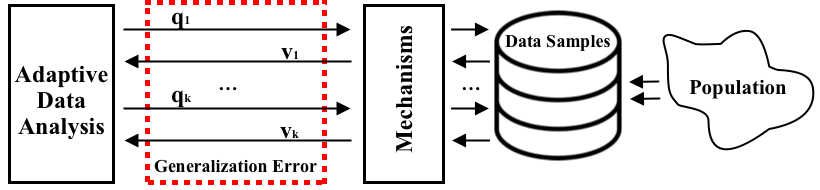
\includegraphics[width=0.7\columnwidth]{overview.png}
    \caption{Overview of our Adaptive Data Analysis model.
    We have a population that we are interested in studying, and a dataset containing individual samples from this population. 
    The adaptive data analysis we are interested in running has access to the dataset through queries of some pre-determined family (e.g., statistical or linear queries) mediated by a mechanism. 
    This mechanism uses randomization to reduce the generalization error of the queries issued to the data.}
    \label{fig:adaptivity-model-overview}
\vspace{-0.5cm}
\end{figure}

A line of work initiated by \cite{DworkFHPRR15}, \cite{HardtU14} posed the question: Can we design \emph{general-purpose} methods that ensure generalization in the presence of adaptivity, together with guarantees on their accuracy?  
The idea that has emerged in these works is to use randomization to help ensure generalization. 
Specifically, these works have proposed to mediate the access of an adaptive data analysis to the data by means of queries from some pre-determined family (we will consider here a specific family of queries often called "statistical" or "linear" queries) that are sent to a  \emph{mechanism} which uses some randomized process to guarantee that the result of the query does not depend too much on the specific
sampled dataset. 
This guarantees that the result of the queries generalizes well. This approach is described in Fig.~\ref{fig:adaptivity-model-overview}.  
This line of work has identified many new algorithmic techniques for ensuring generalization in adaptive data analysis, leading to algorithms with greater statistical power than all previous approaches. Common methods proposed by these works include, the addition of noise to the result of a query, data splitting, etc. Moreover, these works have also identified problematic strategies for adaptive analysis, showing limitations on the statistical power one can hope to achieve. Subsequent works have then further extended the methods and techniques in this approach and further extended the theoretical underpinning of this approach, e.g.~\cite{dwork2015reusable,dwork2015generalization,BassilyNSSSU16,UllmanSNSS18,FeldmanS17,jung2019new,SteinkeZ20,RogersRSSTW20}.

A key development in this line of work is that the best method for ensuring generalization in an adaptive data analysis depends to a large extent on the number of \emph{rounds of adaptivity}, the depth of the chain of queries. 
As an informal example, the program $x \leftarrow q_1(D);y \leftarrow q_2(D,x);z \leftarrow q_3(D,y)$ has three rounds of adaptivity, since $q_2$  depends on $D$ not only directly because it is one of its input but also via the result of $q_1$, which is also run on $D$, and similarly,  $q_3$ depends on $D$ directly but also via the result of $q_2$, which in turn depends on the result of $q_1$.
The works we discussed above showed that, not only does the analysis of the generalization error depend on the number of rounds, but knowing the number of rounds actually allows one to choose methods that lead to the smallest possible generalization error - we will discuss this further in Section~\ref{sec:overview}. 

For example, these works showed that when an adaptive data analysis uses a large number of rounds of adaptivity then a low generalization error can be achieved by a mechanism  
adding to the result of each query Gaussian noise scaled to the number of rounds. When instead  an adaptive data analysis uses a small number of rounds of adaptivity then a low generalization error can be achieved by using more specialized methods, such as data splitting mechanism or the reusable holdout technique from~\cite{DworkFHPRR15}.
To better understand this idea, we show in Fig.~\ref{fig:generalization_errors} three experiments showcasing these situations.
More precisely, in Fig.~\ref{fig:generalization_errors}(a) we show the results of a specific analysis\footnote{We will use formally a program implementing this analysis (Fig.~\ref{fig:overview-example}) as a running example in the rest of the paper.} with two rounds of adaptivity.
This analysis can be seen as a classifier which first runs 400 non-adaptive queries on the first 400 attributes of the data, looking for correlations between the attributes and a label, and then runs one last query which depends on all these correlations.
Without any mechanism the generalization error of the last query is pretty large, and the lower generalization error is achieved when the data-splitting method is used.
Fig.~\ref{fig:generalization_errors}(c) shows how this situation also change with the number of queries. Specifically, it shows the root mean square error of the last \emph{adaptive} query when the numbers queries varies. This also highlight the fact that different mechanisms, for the same analysis, produce results with very different generalization error.
In Fig.~\ref{fig:generalization_errors}(b), we show the results of a specific analysis\footnote{We will present this analysis formally in Section~\ref{sec:examples}.} with four hundreds rounds of adaptivity.
At each step, this analysis runs an adaptive query based on the results of the previous ones. Without any mechanism, the generalization error of most of the queries is pretty large, and this error can be lowered by using Gaussian noise. 
{\small
\begin{figure}
\centering
\begin{subfigure}{.32\textwidth}
\begin{centering}
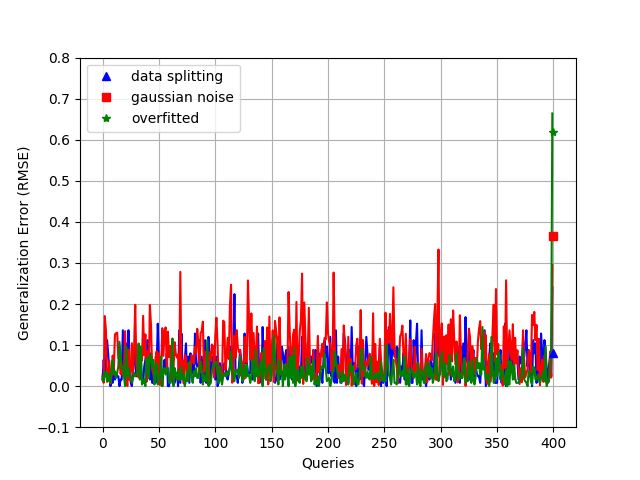
\includegraphics[width=1.0\textwidth]{tworound.png}
\caption{}
\end{centering}
\end{subfigure}
\quad
\begin{subfigure}{.32\textwidth}
\begin{centering}
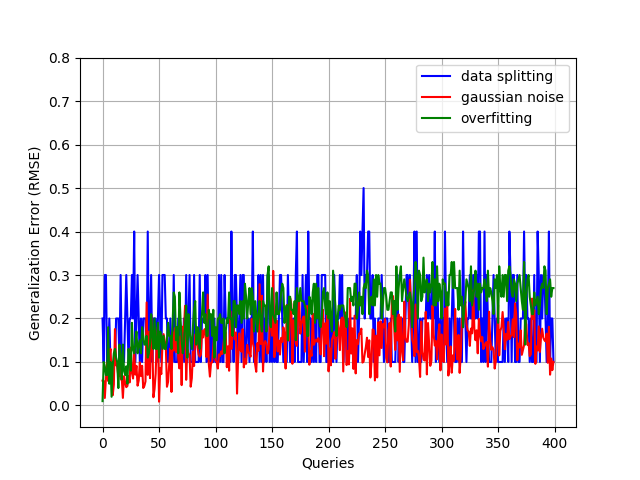
\includegraphics[width=1.0\textwidth]{multipleround.png}
\caption{}
\end{centering}
\end{subfigure}
\begin{subfigure}{.32\textwidth}
\begin{centering}
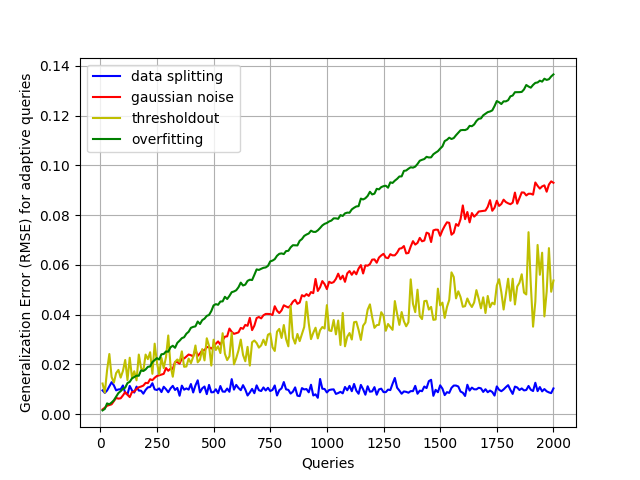
\includegraphics[width=1.0\textwidth]{twoRounds-rmse-fourmechs.png}
\caption{}
\end{centering}
\end{subfigure}
\vspace{-0.5cm}
 \caption{
 The generalization errors of two adaptive data analysis examples, under different choices of mechanisms.
 (a) Data analysis with 2 rounds adaptivity, 
 (b) Data analysis with 400 rounds adaptivity.
 (c) Same Data analysis as (a) with different query numbers.
}
\label{fig:generalization_errors}
\vspace{-0.6cm}
\end{figure}
}
%gap

This scenario motivates us to explore the design of program analysis techniques that can be used to estimate the number of \emph{rounds of adaptivity} that a program implementing a data analysis can perform. These techniques could be used to help a data analyst in the choice of the mechanism to use,
and they
could ultimately be integrated into a tool for adaptive data analysis such as the \emph{Guess and Check} framework by~\cite{RogersRSSTW20}. 

The first problem we face is \emph{how to formally define} a model for adaptive data analysis which is general enough to support the methods we discussed above and which would permit to formulate the notion of adaptivity these methods use. We take the approach of designing a programming framework for submitting queries to some \emph{mechanism} giving access to the data mediated by one of the techniques we mentioned before, e.g., adding Gaussian noise, randomly selecting a subset of the data, using the reusable holdout technique, etc. In this approach, a program models an \emph{analyst} asking a sequence of queries to the mechanism. The mechanism runs the queries on the data applying one of the methods above and returns the result to the program. The program can then use this result to decide which query to run next. Overall, we are interested in controlling the generalization of the query results returned by the mechanism, by means of the adaptivity. 

The second problem we face is \emph{how to define the adaptivity of a given program}.
Intuitively, a query $Q$ may depend on another query $P$, if there are two values that $P$ can return which affect in different ways the execution of $Q$. 
For example, as shown in \cite{dwork2015reusable}, and as we did in our example in Fig.~\ref{fig:generalization_errors}(a), one can design a machine learning algorithm for constructing a classifier which first computes each feature's correlation with the label via a sequence of queries, and then constructs the classifier based on the correlation values. If one feature's correlation changes, the classifier depending on features is also affected.  
This notion of dependency builds on the execution trace as a \emph{causal history}. In particular, we are interested in the history or provenance of a query up until this is executed, we are not then concerned about how the result is used --- except for tracking whether the result of the query may further cause some other query. This is because we focus on the generalization error of queries and not their post-processing. % 
To formalize this intuition as a quantitative program property,
we use a trace semantics recording the execution history of programs on some given input --- and we create a dependency graph, where the dependency between different variables (queries are also assigned to variables) is explicit and track which variable is associated with a query request. We then enrich this graph with weights describing the number of times each variable is evaluated in a program evaluation starting with an initial state. The adaptivity is then defined as the length of the walk visiting most query-related variables on this graph\footnote{Formally, graphs will be well-defined only for terminating programs, this will guarantee that the longest walk is finite}. In other words, we define adaptivity as a \emph{quantitative form of program dependency}.

% \jl{ 
% To define adaptivity in our programming framework, we consider a weighted dependency graph over variables assigned in the program, where each edge is built by a semantics dependency relation between these variables. The dependency relation relies on the trace semantics of our programming framework which records the execution history of programs implementing adaptive data analysis. 
% %The novelty comes from the definition of relation of dependency between nodes, which consists of the edge in the graph. For now, we can think of each node is associated with a variable, storing the value assigned to its variable 
% }
% \jl{The general idea beneath this dependency relation is that modifying the value of some variable in an execution trace will later affect the following execution trace.
% By tracking if a variable is assigned by a query or not, we are able to distinguish whether one query may depend on the other.}

The third problem we face is \emph{how to estimate the adaptivity of a given program}. 
The adaptive data analysis model we consider and our definition of adaptivity suggest that for this task we can use a  program analysis that is based on some form of dependency analysis. This analysis needs to take into consideration:
1) the fact that, in general, a query $Q$ is not a monolithic block but rather it may depend, through the use of variables and values, on other parts of the program. Hence, it needs to consider some form of data flow analysis. 
2) the fact that, in general, the decision on whether to run a query or not may depend on some other value. Hence, 
 it needs to consider some form of control flow analysis.
 3) the fact that, in general, we are not only interested in whether there is a dependency or not, but in the length of the chain of dependencies. Hence, it needs to consider some quantitative information about the program dependencies. 
 
To address these considerations and be able to estimate a sound upper bound on the adaptivity of a program, 
we develop a static program analysis algorithm, named {\THESYSTEM}, which combines data flow and control flow analysis with reachability bound analysis~\cite{GulwaniZ10}. This combination gives tighter bounds on the adaptivity of a program than the ones one would achieve by directly using the data and control flow analyses or the ones that one would achieve by directly using reachability bound analysis techniques alone. We evaluate {\THESYSTEM} on a number of examples showing that it is able to efficiently estimate precise upper bounds on the adaptivity of different programs. 
All the proofs and extended definitions can be found in the supplementary material.

To summarize, our work aims at the design of a static analysis for programs implementing adaptive analysis that can estimate their rounds of adaptivity. Specifically, our contributions are:
\begin{enumerate}
    \item A programming framework for adaptive data analyses where programs represent analysts that can query generalization-preserving mechanisms mediating the access to some data. 
    \item 
    A formal definition of the notion of adaptivity under the analyst-mechanism model. 
    This definition is built on a variable-based dependency graph that is constructed using sets of program execution traces.
    \item 
    A static program analysis algorithm {\THESYSTEM} combining data flow, control flow and  reachability bound analysis in order to provide tight bounds on the adaptivity of a program.
    \item A soundness proof of the program analysis showing that the adaptivity estimated by {\THESYSTEM} bounds the true adaptivity of the program. 
    \item An implementation of {\THESYSTEM} and an experimental evaluation of the bounds this implementation provides on several examples.
\end{enumerate}

\section{Overview}
\label{sec:overview}
% \subsection{Some results in Adaptive Data Analysis}
%\wq{I think we can move this subsection into appendix. Maybe just leave theorm 1.2 and 1.3}
%\jl{I don't agree}
In Adaptive Data Analysis an \emph{analyst} is interested in studying some distribution $\dist$ over some domain $\univ$.  Following previous works~\cite{DworkFHPRR15,HardtU14,BassilyNSSSU16}, we focus on the setting where the analyst is interested in answers to \emph{statistical queries} (also known as \emph{linear queries}) over the distribution.  A statistical query is usually defined by some function $\qquery \from \univ \to [-1,1]$ (often other codomains such as $[0,1]$ or $[-R,+R]$, for some $R$, are considered).  The analyst wants to learn the \emph{population mean}, which is defined as 
$\qquery(\dist) = \ex{\sample \sim \dist}{\qquery(\sample)}$. 
%
We assume that the distribution $\dist$ can only be accessed via a set of \emph{samples} $\sample_1,\dots,\sample_n$ drawn independently and identically distributed (i.i.d.) from $\dist$.  These samples are held by a mechanism $\mech(\sample_1,\dots,\sample_n)$ who receives the query $\query$ and computes an answer 
$\answer \approx \qquery(\dist)$.
%
The na\"ive way to approximate the population mean is to use the \emph{empirical mean}, which (abusing notation) is defined as 
$\qquery(\sample_1,\dots,\sample_n) = \frac{1}{n} \sum_{i=1}^{n} \qquery(X_i)$.
However, the mechanism $M$ can adopt some methods for improving the generalization error $| a- \qquery(\dist)|$.

In this work we consider analysts that ask a sequence of $k$ queries $\qquery_1,\dots,\qquery_k$.  If the queries are all chosen in advance, independently of the answers \highlight{$a_1,\dots,a_k$} of each other, then we say they are \emph{non-adaptive}.  If the choice of each query $\qquery_j$ depends on the prefix $\qquery_1,\answer_1,\dots,\qquery_{j-1},\answer_{j-1}$ then they are \emph{fully adaptive}.  An important intermediate notion is \emph{$\qrounds$-round adaptive}, where the sequence can be partitioned into $\qrounds$ batches of non-adaptive queries.  Note that non-adaptive queries are $1$-round and fully adaptive queries are $k$-round adaptive.

We now review what is known about the problem of answering $r$-round adaptive queries.  
\begin{thm}[\cite{BassilyNSSSU16}] 
\label{thm:nonadapt-adapt}
\begin{enumerate}

\item For any distribution $\dist$, and any $k$ \emph{non-adaptive} statistical queries, \highlight{with high probablity,} 
% $$
$
\max_{j=1,\dots,k} | \answer_j - \qquery_j(\dist) | = O\left( \sqrt{\frac{\log k}{n}}  \right)
% $$
$.
%
\item For any distribution $\dist$, and  any $k$  \emph{$\qrounds$-round adaptive} statistical queries, with $\qrounds \geq 2$, \highlight{with high probablity,} the empirical mean (rounded to an appropriate number of bits of precision)\footnote{With infinite precision even two queries may give unbounded error, when the first query's result encodes the whole data.} satisfies:\\
% $$
$
\max_{j=1,\dots,k} | \answer_j - \qquery_j(\dist) | = O\left( \sqrt{\frac{k}{n}}  \right)
% $$
$
\end{enumerate}
\end{thm}
In fact, these bounds are tight (up to constant factors) which means that even allowing one extra round of adaptivity leads to an exponential increase in the generalization error, from $\log k$ to $k$.

\citet{DworkFHPRR15} and \citet{BassilyNSSSU16} showed that by using carefully calibrated Gaussian noise in order to limit the dependency of a single query on the specific data instance, one 
can actually achieve much stronger generalization error as a function of the number of queries, specifically.
\begin{thm}[\cite{DworkFHPRR15, BassilyNSSSU16}] \label{thm:gaussiannoise} For any distribution $\dist$, any $k$, any $\qrounds \geq 2$ and any \emph{$\qrounds$-round adaptive} statistical queries, if we answer queries with carefully calibrated Gaussian noise, \highlight{with high probablity,}  we have:
\begin{center}
  $
\max_{j=1,\dots,k} | \answer_j - \qquery_j(\dist) | = O\left( \frac{\sqrt[4]{k}}{\sqrt{n}}  \right)
$  
\end{center}
\end{thm}
% Notice that in order to Theorem~\ref{thm:gaussiannoise} has different quantification in that the optimal choice of mechanism depends on the number of queries.  Thus, we need to know the number of queries \emph{a priori} to choose the best mechanism.
More interestingly, \citet{DworkFHPRR15}
also gave a refined bounds that can be achieved with different mechanisms depending on the number of rounds of adaptivity.   \begin{thm}[\cite{DworkFHPRR15}] \label{thm:gaussiannoise2} For any $r$ and $k$, there exists a mechanism such that for any distribution $\dist$, and any $\qrounds \geq 2$ any \emph{$\qrounds$-round adaptive} statistical queries, \highlight{with high probablity,} it satisfies
\begin{center}
  $
\max_{j=1,\dots,k} | \answer_j - \qquery_j(\dist) | = O\left( \frac{r \sqrt{\log k}}{\sqrt{n}}  \right)
$  
\end{center}
\end{thm}
Notice that Theorem~\ref{thm:gaussiannoise2} has different quantification in that the optimal choice of mechanism depends on the number of queries {and number of rounds of adaptivity}.  This suggests that if one knows a good \emph{a priori upper bound on the number of rounds of adaptivity}, one can choose the appropriate mechanism and get a much better guarantee in terms of the generalization error.
As an example, as we can see in Fig.~\ref{fig:generalization_errors}, if we know that an algorithm is 2-rounds adaptive, we can choose data splitting as {the} mechanism, while if we know that an algorithm has many rounds of adaptivity we can choose Gaussian noise. It is worth to stress that by knowing the number of rounds of adaptivity one can also compute a concrete upper bound on the generalization error of a data analysis. This information allows one to have a quantitative, a priori, estimation of the effectiveness of a data analysis. 
This motivates us to design a static program analysis aimed at giving good \emph{a priori} upper bounds on the number of rounds of adaptivity of a program. 

{\small
\begin{figure}
\centering
\begin{subfigure}{.2\textwidth}
\begin{centering}
$
    \begin{array}{l}
    \kw{towRounds(k)} \triangleq \\
           \clabel{ \assign{a}{0}}^{0} ;
            \clabel{\assign{j}{k} }^{1} ; \\
            \ewhile ~ \clabel{j > 0}^{2} ~ \edo ~ \\
            \Big(
             \clabel{\assign{x}{\query(\chi[j] \cdot \chi[k])} }^{3}  ; \\
             \clabel{\assign{j}{j-1}}^{4} ;\\
            \clabel{\assign{a}{x + a}}^{5}       \Big);\\
            \clabel{\assign{l}{\query(\chi[k]*a)} }^{6}\\
        \end{array}
$
\caption{}
\end{centering}
\end{subfigure}
\begin{subfigure}{.4\textwidth}
%}
\qquad
\begin{centering}
\begin{tikzpicture}[scale=\textwidth/16cm,samples=250]
\draw[] (0, 10) circle (0pt) node
{{ $a^0: {}^{\lambda \trace_0. 1}_{0}$}};
\draw[] (0, 7) circle (0pt) node
{\textbf{$x^3: {}^{\lambda \trace_0. \env(\trace_0) k}_{1}$}};
\draw[] (0, 4) circle (0pt) node {{ $a^5: {}^{\lambda \trace_0. \env(\trace_0) k}_{0}$}};
\draw[] (0, 1) circle (0pt) node
{{ $l^6: {}^{\lambda \trace_0. 1}_{1}$}};
% Counter Variables
\draw[] (8, 9) circle (0pt) node {\textbf{$j^1: {}^{\lambda \trace_0. 1}_{0}$}};
\draw[] (8, 6) circle (0pt) node {{ $j^4: {}^{\lambda \trace_0. \env(\trace_0) k}_{0}$}};
%
% Value Dependency Edges:
\draw[ ultra thick, -latex, densely dotted,] (0, 1.5)  -- (0, 3.5) ;
\draw[ ultra thick, -latex, densely dotted,] (0, 4.5)  -- (0, 6.5) ;
\draw[ thick, -latex] (0, 4.5)  to  [out=-230,in=230]  (0, 9.5) ;
\draw[ thick, -Straight Barb] (1.5, 3.8) arc (120:-200:1);
\draw[ thick, -Straight Barb] (9, 6.5) arc (150:-150:1);
\draw[ thick, -latex] (8, 6.5)  -- (8, 8.5) ;
\draw[ thick, -latex] (0, 1.5)  to  [out=-230,in=230]  (0, 9.5) ;
% Control Dependency
\draw[ thick,-latex] (2, 7)  -- (6, 9) ;
\draw[ thick,-latex] (2, 4.5)  -- (6, 9) ;
\draw[ thick,-latex] (2, 7)  -- (6, 6) ;
\draw[ thick,-latex] (2, 4.5)  -- (6, 6) ;
\end{tikzpicture}
\caption{}
\end{centering}
\end{subfigure}
   \begin{subfigure}{.36\textwidth}
   \begin{centering}
   \begin{tikzpicture}[scale=\textwidth/18cm,samples=200]
\draw[] (0, 10) circle (0pt) node
{{ $a^0: {}^1_{0}$}};
\draw[] (0, 7) circle (0pt) node
{\textbf{$x^3: {}^{k}_{1}$}};
\draw[] (0, 4) circle (0pt) node
{{ $a^5: {}^{k}_{0}$}};
\draw[] (0, 1) circle (0pt) node
{{ $l^6: {}^{1}_{1}$}};
% Counter Variables
\draw[] (5, 9) circle (0pt) node {\textbf{$j^1: {}^{1}_{0}$}};
\draw[] (5, 6) circle (0pt) node {{ $j^4: {}^{k}_{0}$}};
%
% Value Dependency Edges:
\draw[ ultra thick, -latex, densely dotted,] (0, 1.5)  -- (0, 3.5) ;
\draw[ ultra thick, -latex, densely dotted,] (0, 4.5)  -- 
% node [left] {\highlight{$\trace_0 \to \env(\trace_0) k $}}
(0, 6.5) ;
\draw[ thick, -latex] (0, 4.5)  to  [out=-230,in=230]  
% node [left] {\highlight{$\trace_0 \to \env(\trace_0) k $}}
(0, 9.5) ;
\draw[ thick, -Straight Barb] (1.5, 3.5) arc (120:-200:1);
\draw[ thick, -Straight Barb] (6.5, 6.5) arc (150:-150:1);
    % The Weight for this edge
    % \draw[](9, 6) node [] {\highlight{$\trace_0 \to \env(\trace_0) k  $}};
\draw[ thick, -latex] (5, 6.5)  -- (5, 8.5) ;
% Control Dependency
\draw[ thick,-latex] (1.5, 7)  -- (4, 9) ;
\draw[ thick,-latex] (1.5, 4)  -- (4, 9) ;
\draw[ thick,-latex] (1.5, 7)  -- (4, 6) ;
\draw[ thick,-latex] (1.5, 4)  -- (4, 6) ;
\draw[ thick, -latex] (0, 1.5)  to  [out=-230,in=230]  (0, 9.5) ;
\end{tikzpicture}
\caption{}
   \end{centering}
   \end{subfigure}
\vspace{-0.4cm}
 \caption{(a) The program $\kw{towRounds(k)}$, an example 
%  of a program 
with two rounds of adaptivity (b) The corresponding execution-based dependency graph (c) The program-based dependency graph from $\THESYSTEM$.
}
\label{fig:overview-example}
% \vspace{-0.8cm}
\end{figure}
}


\subsection{ {\THESYSTEM} formally through an example.}
We illustrate the key technical components of our framework through a simple adaptive data analysis with two rounds of adaptivity.
% They are 1. the query while language for expressing a data analysis formally, 2. the definition of \emph{adaptivity} (\emph{adaptivity} is the short for \emph{rounds of adaptivity} used in the rest of the paper) based on the language semantics, and 3. the static analysis algorithm providing a sound upper bound on a data analysis' adaptivity.
% }
% \detailed{
% In "two rounds strategy" analysis, the analyst asks in total $k+1$ queries to the mechanism in two phases, the symbol $k$ is an input from the data analyst of this strategy and has no limit on the kind, which can be a constant, or a symbol or even an expression such as $(k+3)*2$.
% } 
%
In this analysis, an analyst asks $k+1$ queries to a mechanism in two phases.
In the first phase, the analyst asks $k$ queries and stores the answers that are provided by the mechanism. In the second phase, the analyst constructs a new query based on the results of the previous $k$ queries and sends this query to the mechanism. 
The mechanism is abstract here and our goal is to use static analysis to provide an upper bound on adaptivity to help choose the mechanism.
This data analysis assumes that the data domain $\univ$ 
contains at least $k$ numeric attributes 
(every query in the first phase focuses on one), which we index just by natural numbers.
The implementation of this data analysis in the language of {\THESYSTEM} is presented in Fig.~\ref{fig:overview-example}(a).

The {\THESYSTEM} language extends a standard while language\footnote{Programs components are labeled, so that we can uniquely identify every component.} with a query request constructor denoted $\query$.
 Queries have the form $\query(\qexpr)$, where $\qexpr$ is a special expression (see syntax in Section~\ref{sec:loop_language}) 
representing a function $\from \univ \to U$ on rows \highlight{of the hidden database the corresponding query will ask}.
We use $U$ to denote the codomain of queries and it could be $[-1,1]$, $[0,1]$ or $[-R,+R]$, for some $R$ we consider. This function characterizes the linear query we are interested in running. Indeed, as we discussed in the previous section, linear queries compute the empirical mean of a function on rows 
--- we use $\chi$ to abstract a possible row in the database \highlight{which distinguishes $\univ$ for a domain of a row}.
 As an example, $x \leftarrow \query(\chi[j] \cdot \chi[k])$ computes an approximation, according to the used mechanism, of the empirical mean of the product of the $j^{th}$ attribute and $k^{th}$ attribute, identified by $\chi[j] \cdot \chi[k]$. Notice that we don't materialize the mechanism but we assume that it is implicitly run when we execute the query. 
 In Fig.~\ref{fig:overview-example}(a), the queries inside the while loop correspond to the first phase of the data analysis and compute \highlight{the sum of the empirical mean of
the product of the $j$th attribute with the $k$th attribute}. 
The query outside the loop corresponds to the second phase and computes an approximation of the empirical mean where each record is weighted by the sum of the empirical mean of the first $k$ attributes.


This example is intuitively 2-rounds adaptive since we have two clearly distinguished phases, and the queries that we ask in the first phase do not depend on each other (the query $\chi[j] \cdot \chi[k]$ at line $3$ only relies on the counter $j$ and input $k$), while the last query 
(at line 6) depends on the results of all the previous queries. 
However, capturing this concept formally is surprisingly difficult. The difficulty comes from the fact that a query can depend on the result of another query in multiple ways, by means of data dependency or control dependency.
% \mg{this is weaker than it was in the previous submission.}

%%%%%%%%%%%%%%%%%%%%%%%%%%%%%%%%%%%Some details that might be useful when make passes %%%%%%%%%%%%%%%%%
% \jl{ The $\bullet$ stands for no query, for instance, the second event in the trace $(j, 1, \env(\trace)k , \bullet) $ tells us the assignment at line $1$ does not request a query.} \jl{The third event is a testing event corresponding to the guard of the while loop at line $2$. The evaluation of the query request in the second phase is tracked in }
% % \jl{ 
% The $\bullet$ is a default value for non-query event, 
% for instance, the second event in the trace $(j, 1, K , \bullet) $ tells us the assignment at line $1$ does not request a query.
% The third event is a testing event corresponding to the guard of the while loop at line $2$. The evaluation of the query request in the second phase is tracked in 
% % }
\subsubsection{Adaptivity definition}
\label{sec:adaptivity-informal}
%%%%%%%%%%%%%%%%%%%%%%%%%%%%%%%%%%% Details Below that might be useful when make passes %%%%%%%%%%%%%%%%%
% \detailed{To formally define the adaptivity, we build a directed graph representing the possible dependencies between queries of a program and we call this graph: execution-based dependency graph. The vertices represent the assigned program variables and the edges satisfy the dependency relations between vertices.   Fig.~\ref{fig:overview-example}(b) is the execution dependency graph we build based on the "two rounds strategy program" in Fig.~\ref{fig:overview-example}(a). In brief, the graph is built by collecting the assigned variables with labels of the target program as vertices, which are $a^0$, $j^1$,...$a^5$,$l^6$. We check if there is an edge between two vertices by our dependency relation over two labeled variables (defined in Section~\ref{sec:dep_adaptivity} ). This dependency relation relies on the execution of the program recorded by a trace generated by our trace semantics, which is the reason we call this graph "execution-based". 
% Intuitively from Fig.~\ref{fig:overview-example}(a), the query in the second phase (at line 6) depends on the query results in the first phase stored in $a$ at line 5, and the variable $a$ also relies on the queries at line 3. Correspondingly, we have two edges $(l^6, a^5)$ and $(a^5, x^3)$ in our execution-based dependency graph in Fig.~\ref{fig:overview-example}(b). Besides, we also have special edge which is a circle, to track any variable being updated with its previous value recursively. For instance, the counter $j$ and the variable $a$ are updated based on previous values $k$ times in the first phase and we see two circle edges on $a^5$ and $j^4$.}

The central property we are after in this work is the \emph{adaptivity of a program}. We define formally this notion in three steps, which we will describe in details in Section~\ref{sec:adaptivity}. First, we define a notion of dependency, or better \emph{may-dependency}, between variables. To do this we take inspiration from previous works on dependency analysis and information flow control and we say that a variable \emph{may depend} on another one if changing the execution of the latter can affect the execution of the former. 
We can see in Fig.~\ref{fig:overview-example}(a) that the value of the variable $l$, which corresponds to the result of the execution of the query in the second phase (in the command with label 6), is affected by the value of the variable $x$, which corresponds to the result of the execution of the query at line 3 in the first phase, via the variable $a$.
To formally define this notion of dependency, as in information flow control, we use the execution history of programs recorded by a trace semantics (see Definition~\ref{def:var_dep}).
% \mg{Please, double check that I refer to the right definition. }  

Second, we build an annotated weighted directed graph representing the possible dependencies between labeled variables. We call this graph \emph{semantics-based dependency graph} to stress that this graph summarizes the dependencies we could see if we knew the overall behavior of the program. 
The vertices of the graph are the assigned program variables with the label of their assignments, edges are pairs of labeled variables which satisfy the dependency relations, weights are functions associated with vertices and describe the number of times the assignment corresponding to the vertex is executed when the program is run in a given starting state\footnote{In our trace semantics the state is recorded in the trace, so an initial state is actually represented by an initial trace. We will use this terminology in later sections.}, and the annotations, which we call \emph{query annotations}, are bits associated with vertices and describe if the corresponding assignment comes from a query (1) or not (0).
The \emph{semantics-based dependency graph} of the $\kw{twoRounds(k)}$ program
we gave in Fig.~\ref{fig:overview-example}(a) is described in Fig.~\ref{fig:overview-example}(b) (we use dashed arrows for two edges that will be highlighted in the next step, for the moment these can be considered similar to the other edges---i.e. solid arrows). We have all the variables that are assigned in the program with their labels, and edges representing dependency relations between them. 
For example, we have two edges $(l^6, a^5)$ and $(a^5, x^3)$ describing the dependency between the variables assigned by queries. The vertices $l^6$ and $x^3$ are the only ones with query annotation $1$ (the subscript), since they are the only two variables that are in assignments involving  queries. Notice that the graph contains cycles---in this example it contains two self-loops. These cycles capture the fact that the variables $a^5$ and $j^4$ are updated at every iteration of the loop using their previous values. Cycles are essential to capture mutual dependencies like the ones that are generated in loops. Adaptivity is a quantitative notion, so capturing this form of dependencies is not enough. This is why we also use weights. The weight of a vertex is a function that given an initial state returns a natural number representing 
the number of times the assignment corresponding to a vertex is visited during the program execution starting in this initial state.  
For example, the vertex $l^{6}$ has weight {$\lambda \trace.1$} since for every initial state {$\trace$} the corresponding assignment will be executed one time, the vertex $a^5$ on the other hand has weight {$\lambda \trace. \env(\trace) k$ since the corresponding assignment will be executed a number of times that correspond to the value of $k$ in the initial state $\trace$, and $\env$ is the operator reading value of $k$ from $\trace$.
}

% It is a function which takes an initial state, $\trace_0$ as input,
% then executes the program, and counts the evaluation times of the query request $\clabel{\assign{l}{\query(\chi[k]*a)} }^{6}$ during the execution.
% % returns $1$ for every starting state, since 
% Since this query at line $6$ is outside of any loop, we are expecting this function always return the count $1$ given any initial state.
% The query annotation of this vertex is $1$, which  indicates that 
% $\clabel{\assign{l}{\query(\chi[k] * a)}}^6$ is a query request.
% For another vertex, $a^{5}:{}^{w_{a^{5}}}_0$ in the while loop, we expect its weight function
% returns different counts if the input initial traces have different initial value for $k$.
% Because $\clabel{\assign{a}{x + a}}^{5}$ will be executed different times if the input $k$  is different.
% Its subscript $0$ representing this is a non-query assignment.



% Besides, we also have special edge which is a circle, to track any variable being updated with its previous value recursively. 
% For instance, the loop counter $j$ and the variable $a$ are updated based on previous values $k$ times in the first phase and we see two circle edges on $a^5$ and $j^4$.

%%%%%%%%%%%%%%%%%%%%%%%%%%%%%%%%%%% Details Below that might be useful when make passes %%%%%%%%%%%%%%%%%
% \detailed{The existence of circle edge \jl{(there isn't a name 'circle edge', the terminology is cycle)}
%  allows our graph to express situation when a variable relies on its previous value recursively inside a while loop, but not show how many times of this reliance, which is necessary to define adaptivity. For instance, if we modify our two round example a little bit to make the query $query(\chi[j]\dot \chi[k])$ at line $3$ relies on its previous result to $query(\chi[j]\dot\chi[k] + x)$, then intuitively its adaptivity becomes $k+1$. To this end, we add quantitative information to our graph: weight on every vertex.
% The weight of a vertex is a function that given a starting state returns a natural number representing 
% the number of times the vertex is visited when the program is executed starting from this state.}
% \jl{The existence of cycle
%  allows our graph to handle the while loop.
% When the variable in a while loop relies on its value in the previous iterations, the cycle expresses this reliance.
% But it cannot express the times of this reliance.
% For instance, if we modify the command $3$
% of the $\kw{twoRounds(k)}$ example
% into $\clabel{\assign{x}{\query(\chi[j] \cdot \chi[k] + x)}}^3$. 
% Then $x$ in every iteration relies on the result in the previous iteration
% and the intuitive adaptivity becomes $k+1$. But we don't know the number $k$ by only constructing the edge $x^3 \to x^3$.
% To this end, we add quantitative information to our graph: weight on every vertex.
% The weight of a vertex is a function that given a starting state returns a natural number representing 
% the number of times the vertex is visited during the program execution.
% }
% Each vertex in this graph has a superscript representing its weight, and a subscript $1$ or $0$ telling if the vertex corresponds to a query or not. We will call this subscript a query annotation. 
% For example, in Fig.~\ref{fig:overview-example}(b), the vertex $l^{6}:{}^{w_1}_1$, 
% has weight $w_1$, a constant function which returns $1$ for every starting state, since 
% this query at line $6$ is at most executed once regardless of the initial trace.
% The query annotation of this vertex is $1$, which  indicates that 
% $\clabel{\assign{l}{\query(\chi[k] * a)}}^6$ is a query request.
% Another vertex, $x^{3}:{}^{w_k}_1$, appears in the while loop. 
% It has as weight a function $w_k$ that for every initial state returns the value that $k$ has in this state, since this is also the number the while loop will be iterated. 
% The node $j^{4}:{}^{w_k}_0$ has as a subscript $0$ representing a non-query assignment.
% \jl{
% For example, in Fig.~\ref{fig:overview-example}(b), the vertex $l^{6}:{}^{w_{l^{6}}}_1$, 
% has weight ${w_{l^{6}}}$. It is a function which takes an initial state, $\trace_0$ as input,
% then executes the program, and counts the evaluation times of the query request $\clabel{\assign{l}{\query(\chi[k]*a)} }^{6}$ during the execution.
% % returns $1$ for every starting state, since 
% Since this query at line $6$ is outside of any loop, we are expecting this function always return the count $1$ given any initial state.
% The query annotation of this vertex is $1$, which  indicates that 
% $\clabel{\assign{l}{\query(\chi[k] * a)}}^6$ is a query request.
% For another vertex, $a^{5}:{}^{w_{a^{5}}}_0$ in the while loop, we expect its weight function
% returns different counts if the input initial traces have different initial value for $k$.
% Because $\clabel{\assign{a}{x + a}}^{5}$ will be executed different times if the input $k$  is different.
% Its subscript $0$ representing this is a non-query assignment.
%
%It has as weight a function $w_k$ that for every initial state returns the value that $k$ has in this state, since this is also the number the while loop will be iterated. 
% The node $j^{4}:{}^{w_k}_0$ has as a subscript $0$ representing a non-query assignment.
% }
%%%%%%%%%%%%%%%%%%%%%%%%%%%%%%%%%%% Details Below that might be useful when make passes %%%%%%%%%%%%%%%%%
% \detailed{Since the edges between two vertices represent the fact that one program variable may depend on the other,
% we can define the program adaptivity with respect to a initial trace by means of a walk traversing the graph, visiting each vertex no more than its weight with respect to the initial trace, and visiting as many query nodes as possible.
% Still, look again at our example, we can see that
% in the walk along the dotted arrows,  $l^{6} \to a^5 \to x^3 $, there are $2$ vertices with query annotation $1$ and that this number is maximal, i.e. we cannot find another walk having more than $2$ vertices with query annotation $1$, under the assumption that $k \geq 1$. So the adaptivity of the program in Fig.~\ref{fig:overview-example}(a)  is $2$,
% as expected.
% }
Third, we can finally define adaptivity using the semantics-based dependency graph. We actually define this notion with respect to an initial state $\tau$, since different states can give very different adaptivities.  
We consider 
% the longest walk  that visits each vertex $v$ of the semantics-based dependency graph no more than the value that the weight $w_v$ assign to $\tau$, and visits as many query nodes as possible. 
\highlight{any} \remove{the} walk  that visits each vertex $v$ of the semantics-based dependency graph no more than the value that the weight $w_v$ applying to the initial state $\tau$, and visits the \highlight{maximal} number of query vertices.
The number of query vertices visited is the adaptivity of the program with respect to $\tau$.
Looking again at Fig.~\ref{fig:overview-example}(b), and assuming that $\tau(k) \geq 1$, we can see that the 
walk along the dashed arrows,  $l^{6} \to a^5 \to x^3 $ has two vertices with query annotation $1$, and we cannot find another walk having more than $2$ query vertices,\highlight{ ( $l^{6} \to x^3 $  with $2$ query vertices as well)}. So the adaptivity of the program in Fig.~\ref{fig:overview-example}(a) with respect to $\tau$ is $2$. If we consider an initial state $\tau$ such that $\tau(k)=0$ we have that the adaptivity with respect to $\tau$ is instead $1$. 
%%%%%%Gap: %%%%%%%%%%%%%%%%%%%%%%%%%%%%%%%%%%%%%%%%%%%%%%%%%%%%%%%%%%%%%%%%%%%%%%%%%%%%%%%%%%%%%%%%%%%%%%%%%%%%%%%%%%%%%%%%%%%%%%%%%%%%%%%%%%%%%%%
% \begin{figure}
%     \centering   
%     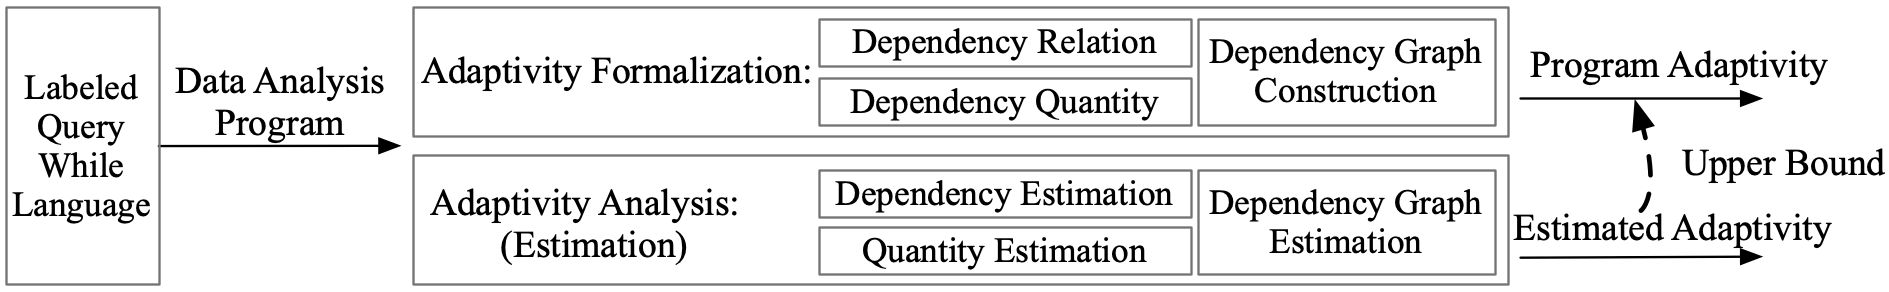
\includegraphics[width=1.0\textwidth]{architecture.png}
%     \vspace{-0.8cm}
%   \caption{High level architecture}
%     \label{fig:structure}
%     \vspace{-0.6cm}
% \end{figure}

\subsubsection{Static analysis}
%%%%%%%%%%%%%%%%%%%%%%%%%%%%%%% Previous Version Below that might be useful when make passes %%%%%%%%%%%%%%%%%
%  \detailed{The definition of adaptivity comes from the aforementioned execution-based dependency graph, 
%  our static analysis statically provides a sound upper bound on this adaptivity, via constructing another weighted graph, we call it estimated dependency graph. The upper bound is then found by searching a sound path with respect to our adaptivity in the generated graph. Different from the execution-based dependency which needs the trace from the execution, estimated one is built by our static analysis algorithm which takes the program itself as input. In brief, our algorithm is consist of a graph-generation algorithm, a weight computation algorithm and finally a path searching algorithm in the generated weighted graph.
%  }
%%%%%%%%%%%%%%%%%%%%%%%%%%%%%%% Previous Version Below that might be useful when make passes %%%%%%%%%%%%%%%%%
% \todo{In order to have a sound and accurate upper bound on the  adaptivity of a program $c$,
% we design a program analysis framework named {\THESYSTEM}.
% This framework composes two algorithms as shown in the double-stroke box and the dashed box in Fig.~\ref{fig:adaptfun}.
% The first algorithm in the double-stroke box combines the quantitative and dependency analysis techniques.
% It produces an estimated \emph{dependency graph} for a program.
% The second algorithm in the dashed box is a walk length estimation algorithm.
% It computes the upper bound on the program's \emph{adaptivity} over the estimated graph.}
% \jl{Since the definition of adaptivity comes from the aforementioned execution-based dependency graph, 
%  our static analysis statically provides a sound upper bound on this adaptivity via approximating this graph. The estimated graph is called \emph{estimated dependency graph}. 
%  The upper bound is then computed by searching the walk in this graph such that it can give a sound bound on the adaptivity.
%  Different from the execution-based dependency graph, the estimated one is produced by our static anlaysis algorithm, which only takes the program as input and does not rely on the execution history.
%  In brief, our algorithm is consist of a weighted graph-generation algorithm and a adaptivity computation algorithm over the graph.
%  }
 
 %%%%%%%%%%%%%%%%%%%%%%%%%%%%%%% Previous Version Above for Reference  %%%%%%%%%%%%%%%%%
To compute statically a sound and accurate upper bound on the \emph{adaptivity} of a program $c$,
we design a program analysis framework named {\THESYSTEM} which we will describe formally in Section \ref{sec:algorithm}. 
The structure of {\THESYSTEM} (Fig.~\ref{fig:adaptfun}) reflects in part the definition of adaptivity we discussed in the previous section. Specifically, {\THESYSTEM} is composed by two algorithms (the ones in dashed boxes in the figure), one for building a dependency graph, which we call \emph{estimated dependency graph}, and the other to estimate the adaptivity from this graph.  
The first algorithm generates the \emph{estimated dependency graph} using several program analysis techniques. Specifically,
 {\THESYSTEM} extracts the vertices and the query annotations by looking at the assigned variables of the program, it estimates the edges by using control flow and data flow analysis, and it estimates the weights by using symbolic reachability-bound analysis---weights in this graph are symbolic expressions over input variables. 
% This combined analysis allow us to obtain more accurate upper bounds than what we would obtain by using any of these single analysis technique in isolation.
The second algorithm estimates the
% longest 
walk which respects the weights and which visits the maximal number of query vertices.
%  as possible. 
The two algorithms together gives us an  upper bound on the program's \emph{adaptivity}.

 \begin{figure}
  \centering    
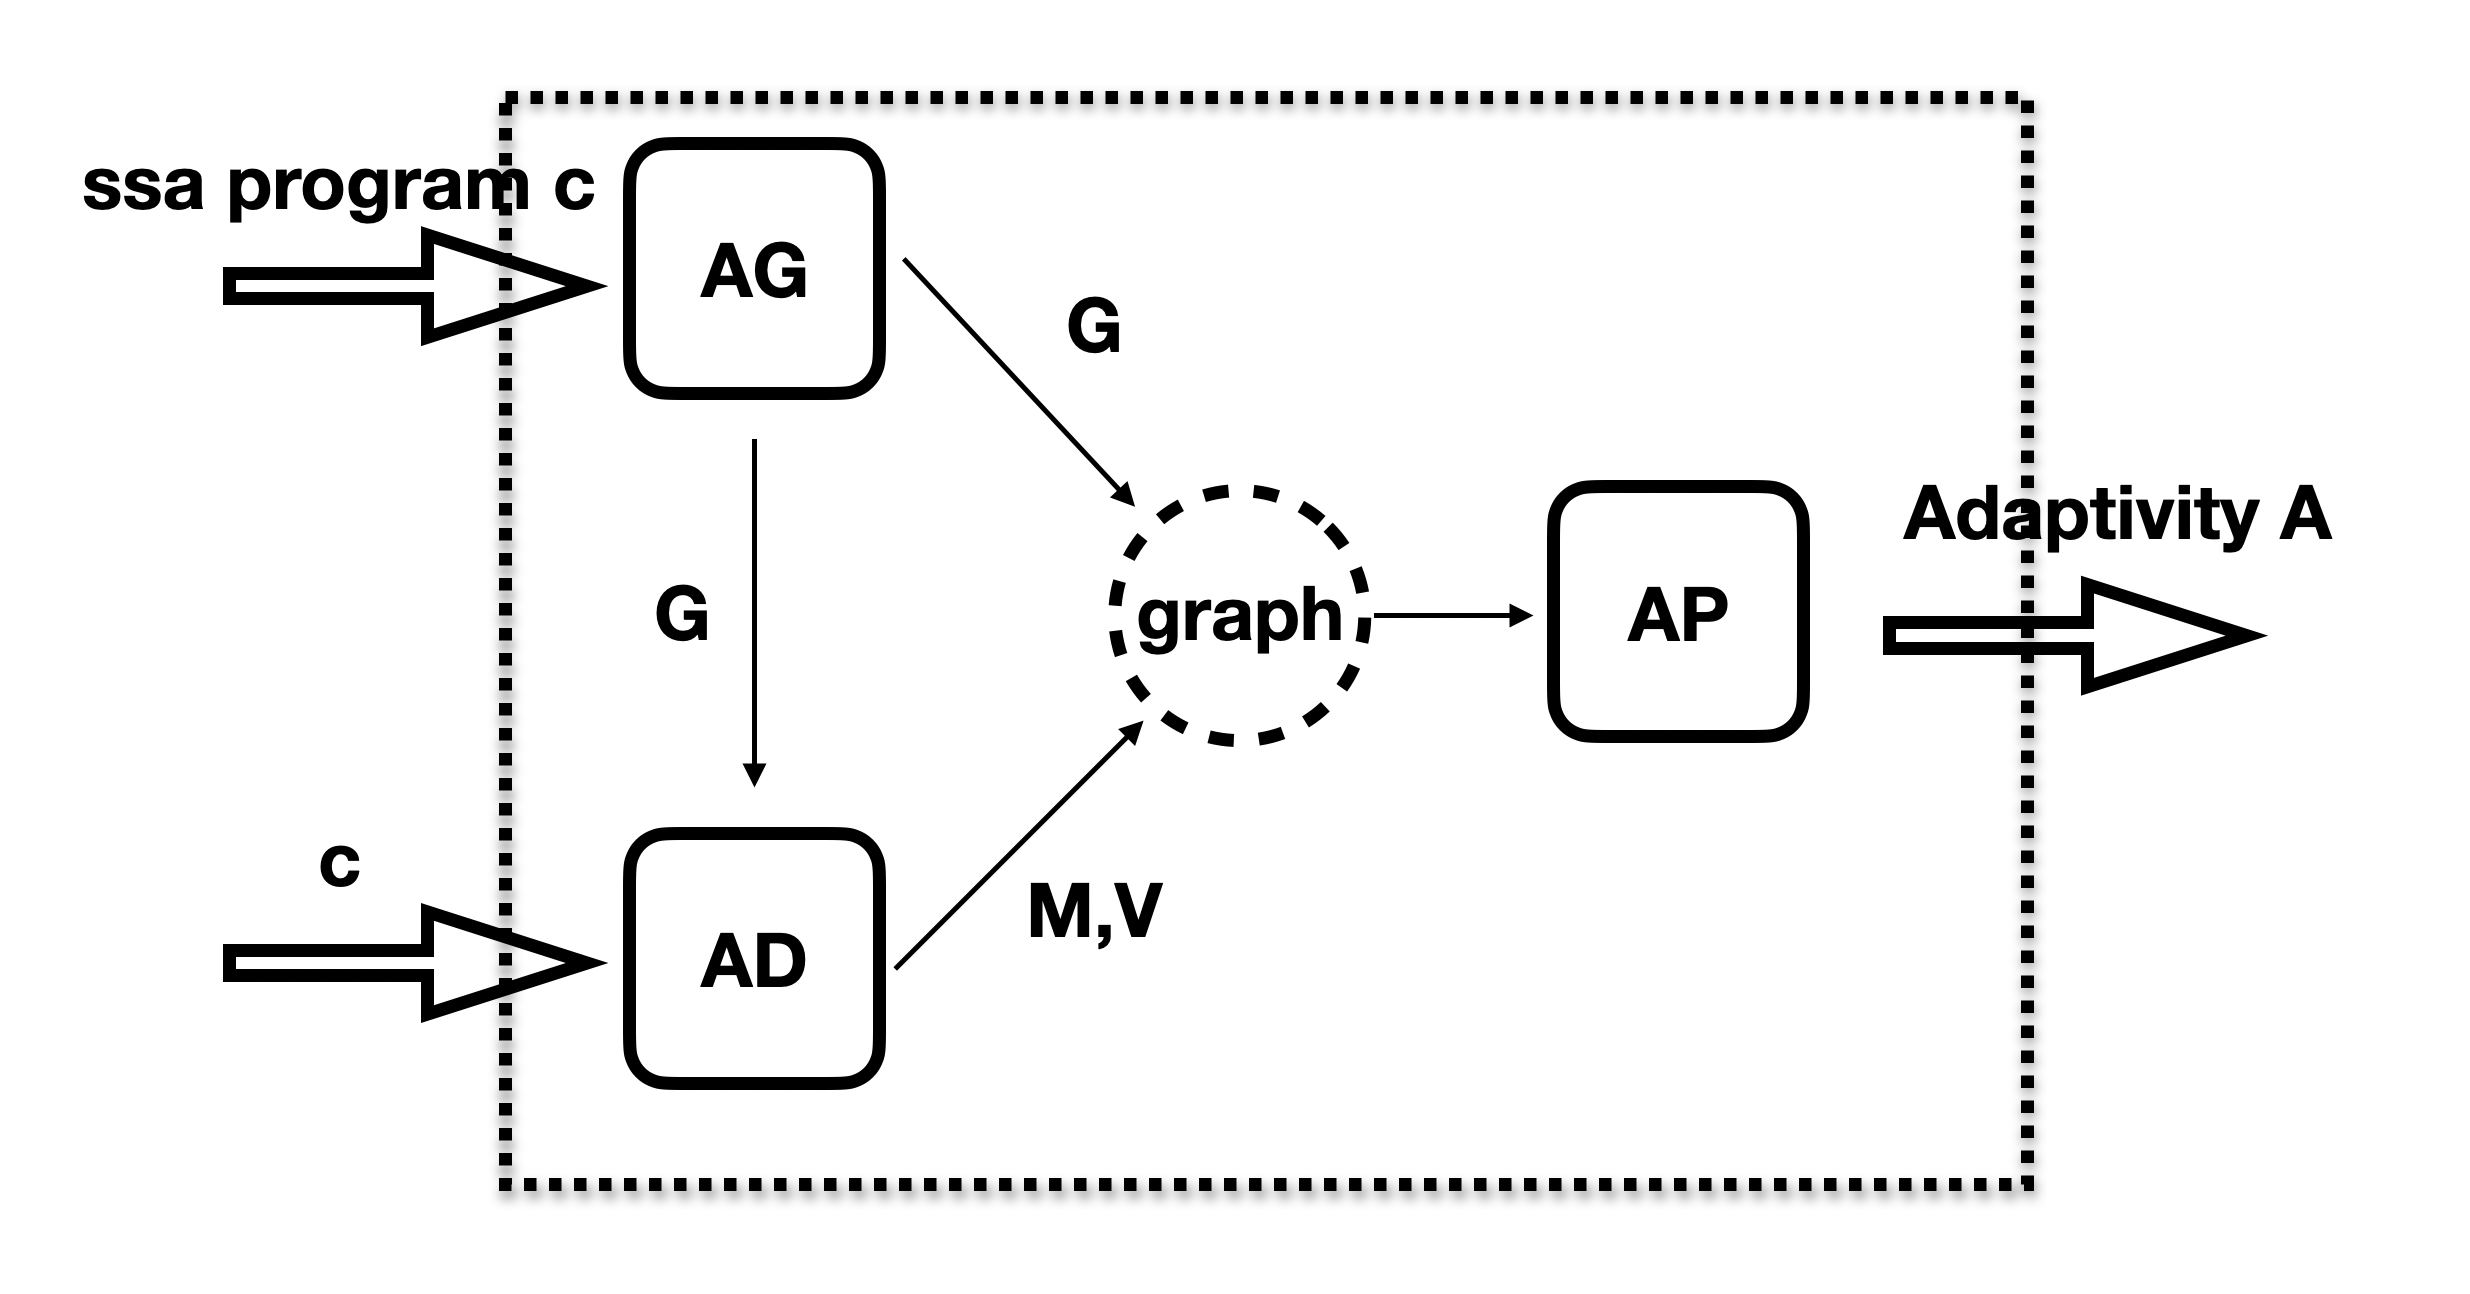
\includegraphics[width=1.0\columnwidth]{adapfun.png}
  \vspace{-0.8cm}
  \caption{The overview of {\THESYSTEM}}
  \label{fig:adaptfun}
  \vspace{-0.5cm}
\end{figure}

 
%%%%%%%%%%%%%%%%%%%%%%%%%%%%%%%%%%% Details Below that might be useful when others are making passes %%%%%%%%%%%%%%%%%
%   \detailed{Fig.~\ref{fig:overview-example}(c) is the resulting estimated graph of our static analysis algorithm which consumes the program in Fig.~\ref{fig:overview-example}(a).The edges are generated by our graph generation algorithm which combines control flow analysis and data flow analysis, presented in Section~\ref{sec:alg_edgegen}). We can easily see the generated graph in Fig.~\ref{fig:overview-example}(c) is a safe approximation of its execution-based counterpart in Fig.~\ref{fig:overview-example}(b), in the way that we can find a corresponding edge in Fig.~\ref{fig:overview-example}(c) for all the edges in Fig.~\ref{fig:overview-example}(b). We call the weight of every vertex computed by our algorithm as estimated weight,  }
%   estimated by using a reachability-bound estimation algorithm (presented in Section~\ref{sec:alg_weightgen}). \detailed{Different from the execution-based weight $w_1$ or $w_k$ in Fig.~\ref{fig:overview-example}(b) which is a function whose output relies on the initial trace, our estimated weight} can be symbolic and provide a sound upper bound on its execution-based weight of the corresponding vertex in the execution-based dependency graph. For instance, 
%   the estimated weight $k$ of the vertex $x^{3}$ in Fig.~\ref{fig:overview-example}(c) is a sound upper bound on the execution-based weight $w_k$ of vertex $x^{3}$ in Fig.~\ref{fig:overview-example}(b), with the same starting trace $\trace$, $w_k(\trace) \leq\trace(k)$. $\trace(k)$ means getting the value of variable $k$ in the trace $\trace$. The soundness of this step is proved in Theorem~\ref{thm:addweight_soundness}.   
%
We show in Fig.~\ref{fig:overview-example}(c) the estimated dependency graph that our static analysis algorithm returns for the program $\kw{twoRounds(k)}$ in Fig.~\ref{fig:overview-example}(a).
Vertices and query annotations are the same as the ones in Fig.~\ref{fig:overview-example}(b) and they are simply inferred by scanning the program.
As we said before, the edges are estimated using control flow and data flow analysis.
For the $\kw{twoRounds(k)}$ example, every edge in Fig.~\ref{fig:overview-example}(b) is precisely inferred by our combined analysis, this is why Fig.~\ref{fig:overview-example}(c) contains exactly the same edges.
The weight of every vertex is computed using a reachability-bound estimation algorithm which outputs a symbolic expression over the input variables, in the example only $k$, representing an upper bound on the number of times each assignment is executed.
% \wq{symbolic and provide a sound upper bound on its execution-based weight of the corresponding vertex in the execution-based dependency graph.
% $w_k(\trace) \leq \trace(k)$. $\trace(k)$ means getting the value of variable $k$ in the trace $\trace$. The soundness of this step is proved in Theorem~\ref{thm:addweight_soundness}.}
For example, consider the vertex $x^{3}$, its weight is $k$ and this provides an upper bound on the value returned by the weight function $\lambda \trace. \rho(\trace)k$ associated with vertex $x^{3}$ in Fig.~\ref{fig:overview-example}(b) for any initial state. 
% Indeed, 
% for any initial trace $\trace_0$, when $w_{x^{3}}(\trace_0)$ executes the program and counts the
% execution times of command $3$,
% we expect that this counts is at most the the loop iterations, i.e. $k$'s initial value from $\trace_0$.

The algorithm searching for the walk first finds a path $l^6:{}^1_1 \to a^5: {}^k_0 \to x^3: {}^k_1$, and then constructs a walk based on this path. Every vertex on this walk is visited once, and the number of vertices with query annotation $1$ in this walk is $2$, which is the upper bound we expect.
{It is worth noting here that $x^3$ and $a^5$ can only be visited once because there isn't an edge to go back to them, even though they both have the weight $k$}.
In this sense, instead of simply computing the weighted length of this path ($2k+1$) as adaptivity, the algorithm $\pathsearch$ computes the upper bound $2$. Note that $2$ is not always tight, for example when $k = 0$.
% \todo{Can you double check if this is clear?}
% \mg{I think we should add a sentence to say that this bound is actually not always tight.}


\section{Loop language }
\label{sec:loop_language}
% In this section, we formally introduce the language we will focus on for writing data analyses.  This is a simple loop language with some primitives for calling queries. After defining the syntax of the language and showing an example, we will define its trace-based operational semantics. This is the main technical ingredient we will use to define the program's adaptivity. We will conclude this section by discussing the limitation of this language with respect to static analysis for adaptivity.

\subsection{Syntax}
\label{subsec:loop-syntax}
{\small
\begin{figure}
\[
\begin{array}{llll}
%  \mbox{Arithmatic Operators} & \oplus_a & ::= & + ~|~ - ~|~ \times 
% %
% ~|~ \div \\  
%   \mbox{Boolean Operators} & \oplus_b & ::= & \lor ~|~ \land ~|~ \neg\\
%   %
%   \mbox{Relational Operators} & \sim & ::= & < ~|~ \leq ~|~ == \\  
%  \mbox{Label} & l & := & \mathbb{N} \\ 
%  \mbox{While Map} & w & \in & \mbox{Label} \times \mathbb{N} \\
\mbox{Arithmetic Expressions} & \aexpr & ::= & 
	%
	n ~|~ x ~|~ \aexpr \oplus_a \aexpr ~|~ \\
% \sep \pi (l , \aexpr, \aexpr) \\
    %
\mbox{Boolean Expressions} & \bexpr & ::= & 
	%
	\etrue ~|~ \efalse  ~|~ \neg \bexpr
	 ~|~ \bexpr \oplus_b \bexpr
	%
	~|~ \aexpr \sim \aexpr \\
\mbox{Expressions } & \expr & ::= & \aexpr \sep \bexpr \sep \chi\sep [] ~|~ [\expr, \dots, \expr] ~|~ \chi[\aexpr] ~|~ x[\aexpr]\\
\mbox{Values } & v & ::= & n \sep \etrue \sep \efalse \sep \chi \sep [] ~|~ [v, \dots, v] ~|~ \chi[v] \\
\mbox{Commands} & c & ::= &  \eskip  ~|~  \assign x \expr ~|~  \assign{x}{ q(e)}
%
~|~ \eloop ~ \aexpr  ~ \edo ~ c  ~|~ c;c  ~|~ \eif(\bexpr, c, c) 	 
	\\
%\mbox{Variables} & \mathcal{VAR}  & ::= & \{ {x} \} \\
%
% \mbox{Trace} & t & ::= & [] ~|~ [(q, v)^{(l, w) }] ~|~ t ++ t
\end{array}
\]
    \vspace{-0.3cm}
 \caption{Syntax of Loop language}
    \label{fig:syntax_highlevel}
    \vspace{-0.5cm}
\end{figure}
}
%
We introduce the syntax of the {\tt Loop} language we use to write our data analyses.
%expression
It is standard that expressions can be either arithmetic expressions or boolean expressions.
An arithmetic expression can be a  constant $n$ denoting integer, a variable $x$ from some countable set $\tt Var$, a combination of arithmetic expressions by means of the symbol $\oplus_a$, denoting basic operations including addition, product, subtraction, etc.
%
A boolean expression can be {\tt true} or {\tt false}, the negation of
a boolean expression, or a combination of boolean expressions by means of $\oplus_b$, denoting basic boolean connectives, or the result of some basic comparison $sym$ between arithmetic expressions, e.g., $\leq,=,<,$ etc. 
Besides, the expression also includes the special variable $\chi$ representing a row of the database, and access to values at a certain index in $\chi$, as $\chi[\aexpr]$. Additionally, list over expressions is supported and $[]$ stands for the empty list. The access to elements in the list can be achieved through $x[\aexpr]$ when variable $x$ is referred to a list. The value $v$ now contains the natural number $n$, the boolean primitives $\etrue$ and $\efalse$, the special row $\chi$ and access to it $\chi[v]$, the empty list $[]$ and non-empty list $[v, \dots, v]$.
% 
%

  A command $c$ can either be $\eskip$, an assignment command $\assign{x}{\expr}$, the composition of two commands $c;c$, an if statement $\eif(\bexpr, c, c)$, a loop statement  $\eloop ~ \aexpr ~ \edo ~ c $.
 The main novelty of the syntax is the query request command $\assign{x}{q(\expr)}$. As a reminder, the aforementioned tight bound of adaptive data analysis in Section~\ref{sec:overview} focuses on linear queries, specified by a function from rows to $[0,1]$ or $[-1,+1]$. To express these functions, we introduce the special variable $\chi$ to represent the rows of the database in the arithmetic expressions. In this sense, a simple linear query which returns the first element of the row is written as $q(\chi[1)])$, representing a query $q(\chi) = \chi(1)$. The query can also take variables as input, the aforementioned two round example in Figure~\ref{fig:simpl-two-round-graph}.(a) uses the loop counter $i$ to construct the query $q(\chi[i])$, and a more complicated one $q(\chi[4]+a)$ at the end.  
 
 
% The query $q(\expr)$ in this command is abstract, and the expression $\expr$ inside the query stores the information of the elements used during the construction of the query. This kind of abstraction of query helps in our analysis and still remain expressive enough for adaptive analysis algorithms. 


% \mg{I don't think that this corresponds exactly to our approach. I think that we want to focus on linear queries, these are the ones for which we have the bounds. A linear query is specified by a function from rows to [0,1] or [-1,+1]. So, in some sense, we want to have a language that describes these functions. Cannot we use $q(r)=e$ where $r$ is a special variable denoting the given row, and $e$ is an expression as we have right now? Example: $q_j(x)=x(i)\cdot x(j)$ can be written as $q(\chi (i)\cdot \chi (j))$ which is a notation for
% $q=\lambda \chi \chi (i)\cdot \chi (j)$.}

%   We have seen a simplified version of the two round algorithm in Section~\ref{sec:overview}. We show its complete version $TRC$ expressed in our {\tt Loop} language on the left hand side in Figure~\ref{fig:tworound_complete}.
 
 
 
 
%  \subsection{An example}
%  \mg{I will not change this section because I think we need to think more about what our language of queries is. As I said above, I think we should be more explicit. For example, I would write $q_1$ as $q(x[j]\cdot x[i])$ or something similar. I also don't think it is a good idea to present Algorithm~\ref{alg:two_round} first, and then show how to write this in our language. We can use two-rounds to introduce our language but I would present it directly in our language without the algorithm. I see several issues in using the algorithm: first, you need to present the example twice, first for the algorithm and then the program; second, the algorithms is not much more real world than other examples - we took it from a research paper which actually now put it in the appendix. I suggest we present the example but only as an example, withouth the algorithm.}

%  We go through a real-world adaptive data analysis algorithm in Algorithm~\ref{alg:two_round}, and see how our high level loop language expresses it. 
 

 
%  \begin{algorithm}
% \caption{A two-round analyst strategy for random data}
%  \label{alg:two_round}
% \begin{algorithmic}
% \REQUIRE Mechanism $\mathcal{M}$ with a hidden state $X\in \{-1,+1\}^{n\times (k+1)}$.
% \STATE  {\bf for}\ $j\in [k]$\ {\bf do}.  
% \STATE \qquad {\bf define} $q_j(x)=x(j)\cdot x(k)$ where $x\in \{-1,+1\}^{k+1}$.
% \STATE \qquad {\bf let} $a_j=\mathcal{M}(q_j)$ 
% \STATE \qquad \COMMENT{In the line above, $\mathcal{M}$ computes approx. the exp. value  of $q_j$ over $X$. So, $a_j\in [-1,+1]$.}
% \STATE {\bf define} $q_{k+1}(x)=\mathrm{sign}\big (\sum_{i\in [k]} x(i)\times\ln\frac{1+a_i}{1-a_i} \big )$ where $x\in \{-1,+1\}^{k+1}$.
% \STATE\COMMENT{In the line above,  $\mathrm{sign}(y)=\left \{ \begin{array}{lr} +1 & \mathrm{if}\ y\geq 0\\ -1 &\mathrm{otherwise} \end{array} \right . $.}
% \STATE {\bf let} $a_{k+1}=\mathcal{M}(q_{k+1})$
% \STATE\COMMENT{In the line above,  $\mathcal{M}$ computes approx. the exp. value  of $q_{k+1}$ over $X$. So, $a_{k+1}\in [-1,+1]$.}
% \RETURN $a_{k+1}$.
% \ENSURE $a_{k+1}\in [-1,+1]$
% \end{algorithmic}
% \end{algorithm}

% As described before, the complete version still has two steps. The query asked in the first step now depends on the iteration number so that the query ask at the $j$ iteration is ($q_j(x) = x(j)\cdot x(k)$), expressed as $q(\chi(j)\cdot \chi(k))$. The iteration counter is initialized to 0, $j = 0$. In the second step, the final query is more complicated. It uses an auxiliary function   $\mathrm{sign}(y)=\left \{ \begin{array}{lr} +1 & \mathrm{if}\ y\geq 0\\ -1 &\mathrm{otherwise} \end{array} \right . $ The input of this function is $\sum_{i\in [k]} \chi(i)\times\ln\frac{1+a[i]}{1-a[i]}$, which sums the product of $\chi(i)$ and $\ln\frac{1+a[i]}{1-a[i]}$ that uses the value at index $i$ of the list $a$.
% \begin{figure}
% \[
% {
% \begin{array}{l}
% \bf{TRC}(k) \\
%     % \left[j \leftarrow 0 \right]^1 ; \\
%     \\
%   \clabel{ a \leftarrow []}^{1} ; \\
%     \clabel{\assign{j}{0} }^{2} ; \\
%     \eloop ~ \clabel{k}^{3} ~ \edo ~ \\
%     \Big(
%      \clabel{x \leftarrow q(\chi(j)\cdot \chi(k)) }^{4}  ; \\
%      \clabel{\assign{j}{j+1}}^{5} ;\\
%     \clabel{a \leftarrow x :: a}^{6}       \Big);\\
%     \clabel{l \leftarrow q(\mathrm{sign}\big (\sum_{i\in [k]} \chi(i)\times\ln\frac{1+a[i]}{1-a[i]} \big ))}^{7}\\
% \end{array} ~~
% {
% \begin{array}{l}
% \bf{TRC^{ssa}}(k) \\
%     % \left[j \leftarrow 0 \right]^1 ; \\ 
%     \\
%     \clabel{a_1 \leftarrow []}^{1} ; \\
%     \clabel{\assign{j_1}{0} }^{2} ; \\
%     \eloop ~ \clabel{k}^{3}, 0, ~ \edo [(j_3, j_1,j_2),(a_3, a_1,a_2)]~ \\
%     \Big(
%     \clabel{ x_1 \leftarrow q(\chi(j_3)\cdot \chi(k))}^{4}  ; \\
%     \clabel{ \assign{j_2}{j_3+1} }^{5} ;\\
%     \clabel{a_2 \leftarrow x_1 :: a_3}^{6}       \Big);\\
%     \clabel{l_1 \leftarrow q(\mathrm{sign}\big (\sum_{i\in [k]} \chi(i)\times\ln\frac{1+a_3[i]}{1-a_3[i]} \big ))}^{7}\\
% \end{array}
% }
% }
% \]  
%     \caption{Two round algorithm complete version}
%     \label{fig:tworound_complete}
% \end{figure}
% The second step of the Algorithm~\ref{alg:two_round} is to use the previous results $a_j$ from mechanism $\mathcal{M}$ for $j \in [k]$ to construct a complicated query $q_{k+1}$. In the high level language, we abstract this complex query as $q_2(a)$, $q_2$ representing queries of this complex kind of form and the argument $a$ is what we need for our analysis.

% In a word, we go through a two-round adaptive analysis algorithm and shows how we can represent it in the {\tt Loop} language. It reveals the expressiveness of this language for most of adaptive data analysis algorithms. 

\subsection{ Trace-based Operational Semantics}
 We evaluate programs in our {\tt Loop} language by means of a trace-based operational semantics, to capture the dependency between queries. For distinguishing elements in the the trace, we add a label to commands in the {\tt Loop} language as follow:
% syntax
% \mg{Change "while map" to "Loop maps" everywhere.}
% \dg{Are you sure that a label map is really of type $\mbox{Label} \times \mathbb{N}$ and not $\mbox{Label} \to \mathbb{N}$? I fail to understand how a single pair of label and $\mathbb{N}$ can represent nested loops. } \wq{It is a map}
%
\[
\begin{array}{llll}
     \mbox{Labeled commands} & c & ::= &   [\assign x \expr]^{l} ~|~  [\assign x q(e)]^{l}
 ~|~  \eloop ~ [\aexpr]^{l} ~ \edo ~ c  ~|~ c;c  ~|~ \eif([\bexpr]^l, c, c) 	 ~|~ [\eskip]^{l} \\
\end{array}
\]

Each command is now labeled with a label $l$, a natural number standing for the line of code where the command appears. Notice that we associate the label $l$ to the conditional predicate $\bexpr$ in the if statement, and to the loop counter $\aexpr$ in the loop statement. We will also use  Loop Maps $w$ as defined below.  
% implicitly this gives us a control flow graph representation for the program,
% which is useful when we define adaptivity in the later section. 
% t, m, w, explanation
\[
\begin{array}{llll}
 \mbox{Loop Maps} & w & \in & \mbox{Label} \to \mathbb{N} \\
% \mbox{Labelled commands} & c & ::= &   [\assign x \expr]^{l} ~|~  [\assign x q(e)]^{l}
%  ~|~  \eloop ~ [\aexpr]^{l} ~ \edo ~ c  ~|~ c;c  ~|~ \eif([\bexpr]^l, c, c) 	 ~|~ [\eskip]^{l} \\
% 	\\ ~|~ [\eswitch( \expr, x, v_i \to  q_i)]^{l}
	%
% \mbox{Binary Operation} & \bop & ::= & + ~|~ - ~|~ \times %
% %
% ~|~ \div ~|~ < ~|~ \leq ~|~ = \\
% %
% \mbox{Unary Operation} & \uop & ::= & \ln ~|~ - \\
% %
% \mbox{Memory} & m & ::= & \emptyset ~|~ (x \to v) :: t \\
%
\mbox{Annotated Query} & \mathcal{AQ}  & ::= & \{ q(v)^{(l,w)}  \} \\
\end{array}
\begin{array}{llll}
    \mbox{Memory} & m & ::= & [] ~|~ m[x \to v] \\
\mbox{Trace} & t & ::= & [] ~|~ q(v)^{(l, w) } :: t \\
\end{array}
\]

% \mg{I suggest to move the definitions of memories to the section on semantics.}
  Loop maps are map from labels $l$ to iteration number $n$.
%   Because statements in the loop share the same line number,  varied iterations , the label $l$ is not enough to distinguish statements.
  A  mapping $[k \to n]$ gives accurate information on which loop a statement is in by its key $k$ (label at loop counter), and which iteration $n$ the statement belongs to. For example, the loop maps $w=[3:1, 4:2]$ indicates that the statement is currently in a nested loop, the outer loop starting from label $3$ and in its first iteration, the statement is now in the inner loop starting from label $4$ and in the second iteration. We use $\emptyset$ to represent an empty map, indicating the statement is not in any loop. We define operations on $w$ as follows.
%  We can understand the annotation in such a way. The label $l$ locates arbitrary query request when we look at the execution path of a program with no loop. However, when loop repeats queries in its body, these query requests from varied iterations share the same line number. Hence, the label $l$ is not enough to distinguish queries in loops. For this purpose, another symbol is needed to represent the iteration number of a loop.
% A simplified approach is to use natural number $n$ for the iteration number so that a pair $(l, n)$ can help, but it fails to support nested loop. This accounts for the appearance of loop maps $w$ into the annotation $(l,w)$. As a map from label $l$ to the iteration number n (a natural number), $w$ gives accurate information on which loop specified by its label and which iteration $n$ the query belongs to. 
\[
\begin{array}{lll}
w \setminus l     & = w  & l \not\in Keys(w)   \\
     & = w_l & Otherwise \\
\end{array}
\begin{array}{llll}
   w + l & = w[l \to 1] & l \not \in Keys(w) \\   
     & = w [l \to w(l)+1] & Otherwise
\end{array}
\]
We use $w \setminus l$ to remove the mapping of the key $l$ from the loop maps $w$. This is used when exiting the loop at line $l$. The special loop maps $w_l$ expresses a map identical to $w$, but without the mapping of label $l$. We record in $w$ the first iteration of a loop marked by label $l$ by assigning $l$ with the iteration $1$. The mapped number increase when going into another iteration of the same loop. We use $Keys(w)$ to return all the keys of the loop maps $w$.

%%% trace, queries
 A memory is standard, a map from variables to values. Queries can be uniquely annotated as $\mathcal{AQ}$, and the annotation $(l,w)$ considers the location of the query by line number $l$ and which iteration the query is at when it appears in a loop statement, specified by $w$. A trace $t$ is a list of annotated queries accumulated along the execution of the program. 
 
 %% trace
A trace can be regarded as the program history, where this history consists of the queries asked by the analyst during the execution of the program. We collect the trace with a trace-based small-step operational semantics based on transitions of the form $ \config{m,c, t, w} \to \config{m', \eskip, t', w'} $. It states that a configuration $\config{m, c, t,w}$ evaluates to another configuration with the trace and loop maps updated along with the evaluation of the command $c$ to the normal form of the command $\eskip$.  A configuration contains four elements: a memory $m$, the command $c$ to be evaluated, a starting trace $t$, a starting loop maps $w$. Most of the time, the loop maps remains empty until the evaluation goes into loops.  We also have the evaluation of arithmetic expressions of the form $\config{m,\aexpr} \aarrow \aexpr' $, evaluating an arithmetic expression $\aexpr$ in the memory $m$, and similar for the boolean expressions $\config{m, \bexpr} \barrow \bexpr'$.   

%
% figure, evaluation rules.
{\footnotesize
\begin{figure}
\begin{mathpar}
\boxed{ \config{m, c, t,w} \xrightarrow{} \config{m', c',  t', w'} \; }
\and
%
{\inferrule
{
 \valr_N > 0
}
{
\config{m, \eloop ~ [\valr_N]^{l}  ~ \edo ~ c ,  t, w }
\xrightarrow{} \config{m, c ;  \eloop ~ [(\valr_N-1)]^{l} ~ \edo ~ c ,  t, (w + l) }
}
~\textbf{low-loop}
}
%
\and
%
\inferrule
{
}
{
\config{m, [\eskip]^{l} ; c_2,  t,w} \xrightarrow{} \config{m, c_2,  t,w}
}
~\textbf{low-seq2}
%
\quad
%
{
\inferrule
{
 \valr_N = 0
}
{
\config{m,  \eloop ~ [\valr_N]^{l} ~ \edo ~ c  ,  t, w }
\xrightarrow{} \config{m, [\eskip]^{l} ,  t, (w \setminus l) }
}
~\textbf{low-loop-exit}
}
\and
%
\inferrule
{
}
{
\config{m,  \eif([\efalse]^{l}, c_1, c_2),  t,w} 
\xrightarrow{} \config{m, c_2,  t,w}
}
~\textbf{low-if-f}
%
~~
% {  Memory \times Com  \times Trace \times WhileMap \Rightarrow^{} Memory \times Com  \times Trace \times WhileMap}
\inferrule
{
\config{m,\expr} \to \expr'
}
{
\config{m, [\assign{x}{q(\expr)}]^l, t, w} \xrightarrow{}  \config{m, [\assign{x}{q(\expr')}]^l, t, w}
}
~\textbf{low-query-e}
%
\and
%
%
\inferrule
{
\config{m, c_1,  t,w} \xrightarrow{} \config{m', c_1',  t',w'}
}
{
\config{m, c_1; c_2,  t,w} \xrightarrow{} \config{m', c_1'; c_2, t',w'}
}
~\textbf{low-seq1}
~~
\inferrule
{
q(v) = v_q
}
{
\config{m, [\assign{x}{q(v)}]^l, t, w} \xrightarrow{} \config{m[ v_q/ x], \eskip,  t \mathrel{++} [q(v)^{(l,w )}],w }
}
~\textbf{low-query-v}
%
% \inferrule
% {
% }
% {
% \config{m, [\assign x v]^{l},  t,w} \xrightarrow{} \config{m[v/x], [\eskip]^{l}, t,w}
% }
% ~\textbf{low-assn}
%
%
%
\and
%
\inferrule
{
\config{ m, \bexpr} \barrow \bexpr'
}
{
\config{m, \eif([\bexpr]^{l}, c_1, c_2),  t,w} 
\xrightarrow{} \config{m,  \eif([\bexpr']^{l}, c_1, c_2),  t,w}
}
~\textbf{low-if}
%
~~~~
%
\inferrule
{
}
{
\config{m, \eif([\etrue]^{l}, c_1, c_2),t,w} 
\xrightarrow{} \config{m, c_1,  t,w}
}
~\textbf{low-if-t}
%
% %
%
\end{mathpar}
    \vspace{-0.3cm}
    \caption{Trace-based operational semantics}
    \label{fig:evaluation}
    \vspace{-0.5cm}
\end{figure}
}
%
% explanation of rules
We give a selection of rules of the trace-based operational semantics in Figure~\ref{fig:evaluation}.
The rule $\textbf{low-query-e}$ evaluates the argument of a query request. When the argument is in normal form, this query will be answered. The rule $\textbf{low-query-v}$ modifies the starting memory $m$ to $m[v_q/x]$ using the answer $v_q$ of the query $q(v)$ from the mechanism, with the trace expanded by appending the query $q(v)$ with the current annotation $(l,w)$. The rule for assignment is standard and the trace remains unchanged. The sequence rule keeps tracking the modification of the trace, and the evaluation rule for if conditional goes into one branch based on the result of the conditional predicate $\bexpr$. The rules for loop modify the loop maps $w$. In the rule $\textbf{low-loop}$, the loop maps $w$ is updated by $w + l$ because the execution goes into another iteration when the condition $v_N >0$ is satisfied. When $v_N$ reaches $0$, the loop exits and the loop maps $w$ eliminates the label $l$ of this loop statement by $w \setminus l$ in the rule $\textbf{low-loop-exit}$.     
%
\subsection{ Query-based Dependency Graph}
%
We define adaptivity through a query-based dependency graph. In our model, an \emph{analyst} asks a sequence of queries to the mechanism, and the analyst receives the answers to these queries from the mechanism. A query is adaptively chosen by the analyst when the choice of this query is affected by answers from previous queries. In this model, the adaptivity we are interested in is the length of the longest sequence of such adaptively chosen queries, among all the queries the data analyst asks to the mechanism.  Also, when the analyst asks a query, the only information the analyst will have will be the answers to previous queries and the state of the program. It means that when we want to know if this query is adaptively chosen, we only need to check whether the choice of this query will be affected by changes of answers to previous queries. There are two possible situations that can  affect the choice of a query,  
either the query argument directly uses the results of previous queries (data dependency), or the control flow of the program with respect to a query (whether to ask this query or not) depends on the results of previous queries (control flow dependency).

As a first step, we give a definition of when one query may depend on a previous query, which is supposed to consider both control dependency and data dependency. We first look at two possible candidates:
\begin{enumerate}
    \item One query may depend on a previous query if and only if a change of the answer to the previous query may also change the result of the query.
    \item One query may depend on a previous query if and only if a change of the answer to the previous query may also change the appearance of the query.
\end{enumerate}

   The first candidate works well by witnessing the result of one query according to the change of the answer of another query. We can easily find that the two queries have nothing to do with each other in a simple example   
%   but vulnerable to queries request protected by differential privacy mechanisms. In our loop language, a query $q(e)$ represents a query request to the database through a mechanism, which add random noise to protect the return results. In this setting, the results of one query will be randomized due to the noise attached by the mechanism which fails the first candidate because witnessing the results of one query can no longer tells whether the change of the results comes from another query or the change of noise of the differential privacy mechanism. For example, suppose we have a program $p$ which requests two simple queries $q_1()$ and $q_2()$ with no arguments as follows.
     $ p = \assign{x}{q(\chi(1))} ; \assign{y}{q(\chi(2))}$. This candidate definition works well with respect to data dependency. However, if fails to handle control dependency since it just monitors the changes to the answer of a query when the answer of previous queries returned change. The key point is that this query may also not be asked because of an analyst decision which depend on the answers of previous queries. An example of this situation is shown in program $p_1$ as follows.
      \[
      p_1 = \assign{x}{q(\chi(1))} ; \eif( x > 2 ,\assign{y}{q(\chi(2))}, \eskip )
   \]
%   Follow the first definition, we may conclude that $q_2()$ depends on $q_1()$ because the query $q_2()$ may return a different result. Nevertheless, we know that this change of return result of $q_2()$ when we change the value returned by $q_1()$ comes from the hidden mechanism(the noise). So $q_1$ and $q_2$ are independent. 
   We choose the second candidate, which performs well by witnessing the appearance of one query $q(\chi(2))$ upon the change of the result of one previous query $q(\chi(1))$ in $p_1$. It considers the control dependency, and at the same, does not miss the data dependency. In particular, the arguments of a query characterizes it. In this sense, if the data used in the arguments changes due to a different answer to a certain previous query, the appearance of the query may change as well. This situation is also captured by our definition. Let us look at another variant of program $p$, $p_2$, in which the queries equipped with functions using previously assigned variables storing answer of its previous query.
    \[
      p_2 = \assign{x}{q(\chi(2))} ; \assign{y}{q(x+\chi(3))}
   \]
    As a reminder, in the {\tt Loop} language, the query request is composed by two components: a symbol $q$ representing a linear query type and the argument $\expr$, which represents the function specifying what the query asks. So we do think $q(\chi(1))$ is different from $q(\chi(2))$. Informally, we think $q(x+\chi(3))$ may depend on the query $q(\chi(2))$, because equipped function of the former $x+\chi(3)$ depend on the data assigned with $q(\chi(2))$. We can see the appearance definition catches data dependency in such a way, since $q(x+\chi(2))$ will not be the same query if the value of $x$ is changed.    
   
   We give a formal definition of query may dependency based on the trace-based operational semantics as follows.
  % formal definition of IND
  \begin{defn}[Query may dependency ]
One query $q(v_2)$ may depend on its previous query $q(v_1)$ in a program $c$, with a starting loop maps $w$, denoted as
$\mathsf{DEP}(q(v_1)^{(l_1, w_1)}, q(v_2)^{(l_2, w_2)}, c,w,m,D)$ if: 
% \dg{I think the following definition describes when $q(v_2)$ depends on $q(v_1)$, not the other way around as stated in the previous sentence. Also, couldn't we look for $q(v_2)^{(l_2,w_2)}$ in $(t_3-t_1)$ instead of $(t_3-t)$ and then get rid of the "To" relation in the next definition?}
\[
  \begin{array}{l}
     \forall  t. \exists m_1,m_3,t_1,t_3.
\config{m, c,  t,w} \rightarrow^{*} \config{m_1, [\assign{x}{q(v_1)}]^{l_1} ; c_2,
  t_1,w_1} \rightarrow \\ \config{m_1[q(v_1)(D)/x], c_2,
  t_1++[q(v_1)^{(l_1, w_1)}], w_1} \rightarrow^{*} \config{m_3, \eskip,
  t_3,w_3} \\  
  \land 
\Big( q(v_1)^{(l_1,w_1)} \in (t_3-t) \land q(v_2)^{(l_2,w_2)} \in (t_3-t_1) \implies  \exists v \in \codom(q(v_1)), m_3', t_3', w_3'.  \\
 \config{m_1[v/x], {c_2}, t_1++[q(v_1)^{(l_1,w_1)}], w_1} \rightarrow^{*} \config{m_3', \eskip, t_3', w_3'} \land (q(v_2)^{(l_2,w_2)}) \not \in (t_3'-t_1)
\Big)\\
\land 
\Big(q(v_1)^{(l_1,w_1)} \in (t_3-t) \land q(v_2)^{(l_2,w_2)} \not\in (t_3-t_1) \implies  \exists v \in \codom(q(v_1)),  m_3', t_3', w_3'. \\
 \config{m_1[v/x], {c_2}, t_1++[q(v_1)^{(l_1,w_1)}], w_1} \rightarrow^{*} \config{m_3', \eskip, t_3', w_3'} \land (q(v_2)^{(l_2,w_2)})  \in (t_3'-t_1)
\Big)
\end{array}
\]
\end{defn}
 %TODO: some more explanation on def 1
%
% \dg{I have a feeling that something is very off here. Consider the program $p_1$ above. For this program, the definition above will say that there is a dependency between $q(\chi(1))$ and $q(\chi(2))$. Now consider the program $p_1' ~=~ \assign{x}{q(\chi(1))} ; \assign{z}{q(\chi(2))} ; \eif( x > 2 ,\assign{y}{z}, \eskip )$. This new program $p_1'$ is semantically equal to $p_1$, yet the definition above will say that in $p_1'$ there is no dependency between $q(\chi(1))$ and $q(\chi(2))$. So, the notion of dependency defined here does not respect semantic equivalence of programs, which is weird because adaptivity is fundamentally a semantic property.}
% \jl{I put doubt on the semantic equivalence here. If out output of the semantics is memory, I don't think they are semantically equivalent.}
%
We give a formal definition of the query-based dependency graph with the formal definition of may dependency between the two queries above.  
% graph definition
\begin{defn}[Query-based Dependency Graph]
Given a program $c$, a database $D$, a starting memory $m$, an initial loop maps $w$, the query-based dependency graph $G(c,D,m,w) = (V, E)$ is defined as: \\
$V =\{q(v)^{l,w} \in \mathcal{AQ} \mid \forall t. \exists m',  w', t'.  \config{m ,c, t, w}  \to^{*}  \config{m' , \eskip, t', w' }  \land q(v)^{l,w} \in {(t'-t)}  \}$.
\\
$E = \left\{(q(v)^{(l,w)},q(v')^{(l',w')}) \in \mathcal{AQ} \times \mathcal{AQ} 
~ \left \vert ~ \mathsf{DEP}(q(v')^{(l',w')},q(v)^{(l,w)}, c,w,m,D)
 \right.\right\}$.
\end{defn}
%
% The function $\mathsf{To}(q(v')^{(l',w')}, q(v)^{(l,w)}$ tells that the query request $q(v')^{(l',w')}$ appears after the query request $q(v)^{(l,w)}$ in the trace, by comparing the annotation $(l',w')$ and $(l,w)$. It helps to decide on the direction of one edge.
The edge is directed, when an annotated query $q(v)^{(l,w)}$ may depend on its previous query $q(v')^{(l',w')}$, we have the directed
edge $(q(v)^{(l,w)}, q(v')^{(l'.w')})$, from $q(v)^{(l,w)} $ to $q(v')^{(l'.w')}$.

The query-based dependency graph only considers the newly generated annotated queries during the execution of the program $c$, so we see the nodes coming from the trace $t'-t$. The previous trace before the execution of $c$ is excluded when constructing the graph. To summary, for every execution of a program $c$ staring with different configurations, we can construct a corresponding dependency graph. 

% adaptivity definition - longest path
Finally, we reach the definition of adaptivity, by means of the query-based dependency graph. 

\begin{defn}[Adaptivity in {\tt Loop} language]
Given a program $c$, and a memory $m$, a database $D$, a starting loop maps $w$, the adaptivity of the dependency graph $G(c, D,m,w) = (V, E)$ is the length of the longest path in this graph. We denote the path from $q(v)^{(l,w)}$ to $q(v')^{(l',w')}$ as $p(q(v)^{(l,w)}, q(v')^{(l',w')} )$. The adaptivity denoted as $A(c, D, m, w)$.
%
$$A(c, D, m, w) = \max\limits_{q(v)^{(l,w)},q(v')^{(l',w')} \in V }\{ |p(q(v)^{(l,w)}, q(v')^{(l',w')} )| \}$$
\end{defn}

% \subsection{ Adaptivity through an example }

%  We still use the two round example in Figure~\ref{fig:simpl-two-round-graph} to illustrate the process of collecting the trace, building the dependency graph and reaching the adaptivity. 

% \[
% TRC(k) \triangleq
% {
% \begin{array}{l}
%     % \left[j \leftarrow 0 \right]^1 ; \\
%   \clabel{ a \leftarrow []}^{1} ; \\
%     \clabel{\assign{j}{0} }^{2} ; \\
%     \eloop ~ \clabel{k}^{3} ~ \edo ~ \\
%     \Big(
%      \clabel{x \leftarrow q(\chi(j)\cdot \chi(k)) }^{4}  ; \\
%      \clabel{\assign{j}{j+1}}^{5} ;\\
%     \clabel{a \leftarrow x :: a}^{6}       \Big);\\
%     \clabel{l \leftarrow q(\mathrm{sign}\big (\sum_{i\in [k]} \chi(i)\times\ln\frac{1+a[i]}{1-a[i]} \big ))}^{7}\\
% \end{array} 
% }
% \]
% \\
% Given a specific database $D = [[1, 1], [0, 0], [1, 1], [1, 1]]$, supposing $a= q_1(\chi[0])(D) +q_1(\chi[1])(D) +q_1(\chi[2])(D) = n$, $n$ is a constant variable $a$ stores in the resulting memory, then the execution trace $t$ is generated along with the operational semantics as follows:
% \\
% $\config{[], TRC(3), D, []>} \to^{*}
% \config{[j \to 3, a \to [1, 0, 1], l \to 1], D, \eskip, t>}$\\
% \[t = \left\{
% q_1(\chi(0))^{(4, [3:1])}, \
% q_1(\chi(1))^{(4, [3:2])}, \ 
% q_1(\chi(2))^{(4, [3:3])}, \ 
% q_2(\chi[4]+n)^{(7, \emptyset)}
% \right \}\]
% For the sake of brevity, we use $q_1(0), q_1(1), q_1(2)$ to represent 
% $ q_1(\chi(0)), 
% q_1(\chi(1)),
% q_1(\chi(2))$. The graph is also shown in Figure~\ref{fig:simpl-two-round-graph}.  


% Then we have the graph as:
% \\
% $V = \left\{
% q_2^6, q_1^{(3,1)}, q_1^{(3,2)}, q_1^{(3,3)}
% \right\}$
% \\
% $E = \left \{
% (q_2^6, q_1^{(3,1)}),
% (q_2^6, q_1^{(3,2)}),
% (q_2^6, q_1^{(3,3)})
% \right\}$
% Then we have the dependency graph generated in Figure \ref{fig:two-round-graph}. 
% \\
% $V = \left\{
% q_{1}(0, 3)^{(3, [1])}, \
% q_{1}(1, 3)^{(3, [2])}, \ 
% q_{1}(2, 3)^{(3, [3])}, \ 
% q_{2}([1, 0, 1])^{(6, [])}
% \right \}$

% Todo: A graph for two round algorithm
% \begin{figure}
% %\begin{figure}
% \begin{tikzpicture}[scale=\textwidth/30cm,samples=200]
% %%% The nodes represents the k query in the first round
% \filldraw[black] (0, 4) circle (5pt) node [anchor=south]{$q_0^{(3,[3:1])}$};
% \filldraw[black] (6, 4) circle (5pt) node [anchor=south]{$q_1^{(3,[3:2])}$};
% \filldraw[black] (12, 4) circle (5pt) node [anchor=south]{$q_2^{(3,[3:3])}$};
% \filldraw[black] (6, 0) circle (5pt) node [anchor=north]{$q(v)^{(7,\emptyset)}$};
% \draw[very thick,->, blue] (6, 0)  -- (6, 3.9) ;
% \draw[very thick,->, red] (6, 0)  -- (12, 3.9) ;
% \draw[very thick,->, blue] (6, 0)  -- (0, 3.9) ;
% \end{tikzpicture}
% \caption{A query-based dependency graph for two round algorithm complete version}
% \label{fig:two-round-graph}
% \end{figure}
%\end{figure}
% Even though the high level loop language provides necessary information for static analysis on most real-world data analysis algorithms, it is not suitable to conduct a static analysis directly on. To be specific, it is challenging to achieve a formal definition of the number of rounds of adaptivity for algorithms using the high level language due to the characteristics depicted in its syntax: the execution of one query $q(e)$ in a program $p$ is decided not only by its explicit control flow (e.g. if statement), but also by its argument $e$. 
%
% Then we have the adaptivity calculated from the graph as:
% \[
% \begin{array}{ll}
% A^*(TR, D, m, w) & = \max\limits_{q(v)^{(l,w)},q'(v')^{(l',w')} \in V }\{ |p(q(v)^{(l,w)}, q'(v')^{(l',w')} )| \}\\
% & = |p(q_2^6, q_1^{(3,3)})| = |p(q_2^6, q_1^{(3,1)})| = |p(q_2^6, q_1^{(3,2)})|\\
% & = 1
% \end{array}
% \]
% We can notice the complete version generates the similar query-based dependency graph as its simplified version in Figure~\ref{fig:simpl-two-round-graph}.


\section{Labeled Language}
%
%
\subsection{Labeled Language}
\[
\begin{array}{llll}
\mbox{Arithmetic Operators} 
& \oplus_a & ::= & + ~|~ - ~|~ \times 
%
~|~ \div \\  
\mbox{Boolean Operators} 
& \oplus_b & ::= & \lor ~|~ \land
\\
%
\mbox{Relational Operators} 
& \sim & ::= & < ~|~ \leq ~|~ == 
\\  
%
\mbox{Label} 
& l & := & \mathbb{N} 
\\ 
%
\mbox{Arithmetic Expression} 
& \aexpr & ::= & 
n ~|~ {x} ~|~ \aexpr \oplus_a \aexpr  
\\
%
\mbox{Boolean Expression} & \bexpr & ::= & 
%
\etrue ~|~ \efalse  ~|~ \neg \bexpr
 ~|~ \bexpr \oplus_b \bexpr
%
~|~ \aexpr \sim \aexpr 
\\
%
\mbox{Expression} & \expr & ::= & v ~|~ \aexpr \sep \bexpr ~|~ [\expr, \dots, \expr]
\\  
%
\mbox{Value} 
& v & ::= & { n \sep \etrue \sep \efalse ~|~ [] ~|~ [v, \dots, v]}  
\\
%
\mbox{Query Expression} 
& {\qexpr} & ::= 
& { \qval ~|~ \aexpr ~|~ \qexpr \oplus_a \qexpr ~|~ \chi[\aexpr]} 
\\
%
\mbox{Query Value} & \qval & ::= 
& {n ~|~ \chi[n] ~|~ \chi[n] \oplus_a  \chi[n] ~|~ n \oplus_a  \chi[n]
~|~ \chi[n] \oplus_a  n}
\\
%
\mbox{Labeled Command} 
& {c} & ::= &   [\assign {{x}}{ {\expr}}]^{l} ~|~  [\assign {{x} } {{\query(\qexpr)}}]^{l}
~|~ {\ewhile [ \bexpr ]^{l} \edo {c} }
\\
&&&
~|~ {c};{c}  
~|~ \eif([\bexpr]{}^l , {c}, {c}) 
~|~ [\eskip] 
\\
%
\mbox{Event} 
& \event & ::= & 
    ({x}, l, v) ~|~ ({x}, l, \qval, v)  ~~~~~~~~~~~ \mbox{Assignment Event} \\
&&& ~|~(\bexpr, l, v)   ~~~~~~~~~~~~~~~~~~~~~~~~~~~~~~~~~~ \mbox{Testing Event}
\\
%
% \mbox{Trace} & \trace
% & ::= & \cdot | \trace \cdot \event | \trace \tracecat \trace 
% \\
%
\mbox{Trace} & \trace
& ::= & [] ~|~ \event:: \trace ~|~ \trace \tracecat \trace  % \\
% %
% \mbox{Event Signature} & \sig
% & ::= & (x, l, n) | (x, l, n, \query) | (b, l, n)
% \\
% %
\end{array}
\]
% \todo{change trace notation into list, and update corresponding operator nations}
% \\
% \wqside{"$\cdot$" has two meanings? empty, delimit. Trace is list of event?}
We use following notations to represent the set of corresponding terms:
\[
\begin{array}{lll}
\mathcal{SVAR} & : & \mbox{Set of Variables}  
\\ 
%
\mathcal{VAL} & : & \mbox{Set of Values} 
\\ 
%
\mathcal{QVAL} & : & \mbox{Set of Query Values} 
\\ 
%
\cdom & : & \mbox{Set of Commands} 
\\ 
%
\eventset  & : & \mbox{Set of Events}  
\\
%
\eventset^{\asn}  & : & \mbox{Set of Assignment Events}  
\\
%
\eventset^{\test}  & : & \mbox{Set of Testing Events}  
\\
%
%%
\dbdom  & : & \mbox{{Set of Databases}} 
\\
%
{\mathcal{T}} & : & \mbox{Set of Traces}
\\
%
\qdom = {[-1,1]} & : & \mbox{{Domain of Query Results}}
\end{array}
\]
%
%
%
Environment $ \env : {\mathcal{T}}  \to \mathcal{SVAR} \to \mathcal{VAL} \cup \{\bot\}$
\[
\begin{array}{lll}
\env(\trace  \tracecat [(x, l, v)]) x \triangleq v
&
\env(\trace \tracecat [(x, l, \qval, v)]) x \triangleq v
&
\env(\trace \tracecat [(y, l, v)]) x \triangleq \env(\trace) x
\\
\env(\trace \tracecat [(b, l, v)]) x \triangleq \env(\trace) x
&
\env({[]} ) x \triangleq \bot
&
\end{array}
\]
%
%
% Query Environment $\qenv: \mathcal{T}  \to \mathcal{SVAR} \to \mathcal{QVAL} \cup \{\bot\}$
% \[
% \begin{array}{lll}
% \qenv(\trace \cdot (x, l, n, v) ) x \triangleq \qenv(\trace) x
% &
% \qenv(\trace \cdot (x, l, n, \qval, v) ) x \triangleq \qval
% &
% \qenv(\trace \cdot (y, l, n, v)) x \triangleq \env(\trace) x
% \\
% \qenv(\trace \cdot (b, l, n, v)) x \triangleq \env(\trace) x
% &
% \qenv(\cdot ) x \triangleq \bot
% &
% \end{array}
% \]
%

%
\subsection{Trace-based Operational Semantics for Language}
%
%
%
{
\begin{mathpar}
\boxed{ \config{\trace,\aexpr} \aarrow v \, : \, \mbox{Trace  $\times$ Arithmetic Expr $\Rightarrow$ Arithmetic Value} }
\\
\boxed{ \config{\trace, \bexpr} \barrow v \, : \, \mbox{Trace $\times$ Boolean Expr $\Rightarrow$ Boolean Value} }
\\
\boxed{ \config{\trace, \expr} \earrow v \, : \, \mbox{Trace $\times$ Expression $\Rightarrow$ Value} }
\\
\inferrule{ 
  \config{\trace, \aexpr} \aarrow v
}{
 \config{\trace,  \aexpr} 
 \earrow v
}
\and
\inferrule{ 
  \config{\trace, \bexpr} \barrow v
}{
 \config{\trace,  \bexpr} 
 \earrow v
}
\and
\inferrule{ 
  \config{\trace, \expr_1} \earrow v_1
  \cdots
  \config{\trace, \expr_n} \earrow v_n
}{
 \config{\trace,  [\expr_1, \cdots, \expr_n]} 
 \earrow [v_1, \cdots, v_n]
}
\and
\inferrule{ 
  \empty
}{
 \config{\trace,  v} 
 \earrow v
}
\\
\boxed{ \config{\trace, \qexpr} \qarrow \qval \, : \, \mbox{Trace  $\times$ Query Expr $\Rightarrow$ Query Value} }
\\
\inferrule{ 
  \config{\trace, \aexpr} \aarrow n
}{
 \config{\trace,  \aexpr} 
 \qarrow n
}
\and
\inferrule{ 
  \config{\trace, \qexpr_1} \qarrow \qval_1
  \and
  \config{\trace, \qexpr_2} \qarrow \qval_2
}{
 \config{\trace,  \qexpr_1 \oplus_a \qexpr_2} 
 \qarrow \qval_1 \oplus_a \qval_2
}
\and
\inferrule{ 
  \config{\trace, \aexpr} \aarrow n
}{
 \config{\trace, \chi[\aexpr]} \qarrow \chi[n]
}
\and
\inferrule{ 
  \empty
}{
 \config{\trace,  \qval} 
 \qarrow \qval
}
 \end{mathpar}
%
The trace based operational semantics are defined in Figure \ref{fig:os_ssa}.
%
\begin{figure}
{
\begin{mathpar}
\boxed{
\mbox{Command $\times$ Trace}
\xrightarrow{}
\mbox{Command $\times$ Trace}
}
\and
\boxed{\config{{c, \trace}}
\xrightarrow{} 
\config{{c',  \trace'}}
}
\\
%
\inferrule
{
\event = ({x}, l, v)
}
{
\config{[\assign{{x}}{\aexpr}]^{l},  \trace } 
\xrightarrow{} 
\config{\eskip, \trace \tracecat [\event ]}
}
~\textbf{assn}
%
\and
%
{
\inferrule
{
 \trace, \qexpr \qarrow \qval
 \and 
\query(\qval) = v
\and 
\event = ({x}, l, \qval, v)
}
{
\config{{[\assign{x}{\query(\qexpr)}]^l, \trace}}
\xrightarrow{} 
\config{{\eskip,  \trace \tracecat[ \event]} }
}
~\textbf{query}
}
%
\and
%
\inferrule
{
 \trace, b \barrow \etrue
 \and 
 \event = (b, l, \etrue)
}
{
\config{{\ewhile [b]^{l} \edo c, \trace}}
\xrightarrow{} 
\config{{
c; \ewhile [b]^{l} \edo c,  \eskip),
\trace \tracecat [\event]}}
}
~\textbf{while-t}
%
%
\and
%
\inferrule
{
 \trace, b \barrow \efalse
 \and 
 \event = (b, l, \efalse)
}
{
\config{{\ewhile [b]^{l}, \edo c, \trace}}
\xrightarrow{} 
\config{{
[\eskip]^l ,
\trace \tracecat [\event]}}
}
~\textbf{while-f}
%
%
\and
%
%
\inferrule
{
\config{{c_1, \trace}}
\xrightarrow{}
\config{{c_1',  \trace'}}
}
{
\config{{c_1; c_2, \trace}} 
\xrightarrow{} 
\config{{c_1'; c_2, \trace'}}
}
~\textbf{seq1}
%
\and
%
\inferrule
{
  \config{{c_2, \trace}}
  \xrightarrow{}
  \config{{c_2',  \trace'}}
}
{
\config{{\eskip ; c_2, \trace}} \xrightarrow{} \config{{ c_2', \trace'}}
}
~\textbf{seq2}
%
\and
%
%
\inferrule
{
   \trace, b \barrow \etrue
 \and 
 \event = (b, l, \etrue)
}
{
 \config{{
\eif([b]^{l}, c_1, c_2), 
\trace}}
\xrightarrow{} 
\config{{c_1, \trace \tracecat [\event]}}
}
~\textbf{if-t}
%
\and
%
\inferrule
{
 \trace, b \barrow \efalse
 \and 
 \event = (b, l, \efalse)
}
{
\config{{\eif([b]^{l}, c_1, c_2), \trace}}
\xrightarrow{} 
\config{{c_2, \trace \tracecat [\event]}}
}
~\textbf{if-f}
% %
%
%
\end{mathpar}
}
% \end{subfigure}
    \caption{Trace-based Operational Semantics for Language.}
    \label{fig:os_ssa}
\end{figure}
%
%
%
%
%
%
%
\clearpage
\clearpage
% %
\section{Event and Trace}
%
%
We have two kinds of events: \emph{assignment events} and \emph{testing events}. 
Each event consists of a quadruple,
and we use $\eventset^{\asn}$ and $\eventset^{\test}$ to denote the set of all assignment events and testing events, respectively.
\begin{center}
$ \begin{array}{lllll}
\mbox{Event} 
& \event & ::= & 
({x}, l, v, \bullet) ~|~ ({x}, l, v, \qval)  & \mbox{Assignment Event} \\
&&& ~|~(\bexpr, l, v, \bullet)  & \mbox{Testing Event}
\\
\end{array}$
\end{center}
An assignment event tracks the execution of an assignment  or a query request and consists of the assigned variable, the label of the command that generates it, the value assigned to the variable, and the normal form of the query expression, $\qval$ if this command is a query request, otherwise a default value $\bullet$.
A testing event tracks the execution of if and while commands and consists of the guard of the command, the label of the command, the result of evaluating the guard, while the last element is $\bullet$.
%

Event projection operators $\pi_i$ projects the $i$th element from an event: 
\\
$\pi_i : 
\eventset \to \mathcal{VAR}\cup \mbox{Boolean Expression}  \cup \mathbb{N} \cup \mathcal{VAL} \cup \mathcal{QVAL} $ 
% \wqside{use b for Boolean expression?}

%
\begin{defn}[Equivalence of Query Expression]
%
\label{def:query_equal}
% \mg{Two} \sout{2} 
Two query expressions $\qexpr_1$, $\qexpr_2$ are equivalent, denoted as $\qexpr_1 =_{q} \qexpr_2$, if and only if
% $$
%  \begin{array}{l} 
%   \exists \qval_1, \qval_2 \in \mathcal{QVAL} \st \forall \trace \in \mathcal{T} \st
%     (\config{\trace,  \qexpr_1} \qarrow \qval_1 \land \config{\trace,  \qexpr_2 } \qarrow \qval_2) 
%     \\
%     \quad \land (\forall D \in \dbdom, r \in D \st 
%     \exists v \in \mathcal{VAL} \st 
%           \config{\trace, \qval_1[r/\chi]} \aarrow v \land \config{\trace,  \qval_2[r/\chi] } \aarrow v)  
%   \end{array}.
% $$
$$
 \begin{array}{l} 
   \forall \trace \in \mathcal{T} \st \exists \qval_1, \qval_2 \in \mathcal{QVAL} \st
    (\config{\trace,  \qexpr_1} \qarrow \qval_1 \land \config{\trace,  \qexpr_2 } \qarrow \qval_2) 
    \\
    \quad \land (\forall D \in \dbdom, r \in D \st 
    \exists v \in \mathcal{VAL} \st 
          \config{\trace, \qval_1[r/\chi]} \aarrow v \land \config{\trace,  \qval_2[r/\chi] } \aarrow v)  
  \end{array}.
$$
% \mg{$$
%  \begin{array}{l} 
%    \forall \trace \in \mathcal{T} \st \exists \qval_1, \qval_2 \in \mathcal{QVAL} \st
%     (\config{\trace,  \qexpr_1} \qarrow \qval_1 \land \config{\trace,  \qexpr_2 } \qarrow \qval_2) 
%     \\
%     \quad \land (\forall D \in \dbdom, r \in D \st 
%     \exists v \in \mathcal{VAL} \st 
%           \config{\trace, \qval_1[r/\chi]} \aarrow v \land \config{\trace,  \qval_2[r/\chi] } \aarrow v)  
%   \end{array}.
% $$
% }
 %
 where $r \in D$ is a row of the hidden database $\chi$, and $\chi$ is in the database domain $D$. 
 As usual, we will denote by $\qexpr_1 \neq_{q} \qexpr_2$  the negation of the equivalence.
% \\ 
% where $r \in D$ is a record in the database domain $D$,
% \mg{is  $FV(\qexpr)$ being defined here? If yes, I suggest to put it in a different place, rather than in the middle of another definition.} 
% $FV(\qexpr)$ is the set of free variables in the query expression $\qexpr$.
% \sout{$\qexpr_1 \neq_{q}^{\trace} \qexpr_2$  is defined vice versa.}
% \mg{As usual, we will denote by $\qexpr_1 \neq_{q}^{\trace} \qexpr_2$  the negation of the equivalence.}
%
\end{defn}
%
% \mg{In the next definition you don’t need the subscript e, it is clear that it is equivalence of events by the fact that the elements on the two sides of = are events. That is also true for query expressions. Also, I am confused by this definition. What happen for two query events?}
% \\
% \jl{The last component of the event is equal based on Query equivalence, $\pi_{4}(\event_1) =_q \pi_{4}(\event_2)$.
% In the previous version, the query expression is in the third component and I defined $v \neq \qexpr$ for all $v$ that isn't a query value.}
% \begin{defn}[Event Equivalence $\eventeq$]
% Two events $\event_1, \event_2 \in \eventset$ \mg{are equivalent, \sout{is in \emph{Equivalence} relation,}} denoted as $\event_1 \eventeq \event_2$ if and only if:
% \[
% \pi_1(\event_1) = \pi_1(\event_2) 
% \land  
% \pi_2(\event_1) = \pi_2(\event_2) 
% \land
% \pi_{3}(\event_1) = \pi_{3}(\event_2)
% \land 
% \pi_{4}(\event_1) =_q \pi_{4}(\event_2)
% \]
% %
% % \sout{The $\event_1 \eventneq \event_2$ is defined as vice versa.}
% % \mg{As usual, we will denote by $\event_1 \eventneq \event_2$  the negation of the equivalence.}
% \end{defn}
\begin{defn}[Event Equivalence]
  Two events $\event_1, \event_2 \in \eventset$ are equivalent, 
  % denoted as $\event_1 \eventeq \event_2$ 
  denoted as $\event_1 = \event_2$ 
  if and only if:
  \[
  \pi_1(\event_1) = \pi_1(\event_2) 
  \land  
  \pi_2(\event_1) = \pi_2(\event_2) 
  \land
  \pi_{3}(\event_1) = \pi_{3}(\event_2)
  \land 
  \pi_{4}(\event_1) =_q \pi_{4}(\event_2)
  \]
  %
  As usual, we will denote by $\event_1 \neq \event_2$  the negation of the equivalence.
\end{defn}
%
\subsection{Trace}
%
% An event $\event \in \eventset$ belongs to a trace $\trace$, i.e., $\event \eventin \trace$ are defined as follows:
% %
% \begin{equation}
%   \event \eventin \trace  
%   \triangleq \left\{
%   \begin{array}{ll} 
%     \etrue                  & \trace =  (\trace' \tracecate \event') \land (\event \eventeq \event') \\
%     \event \eventin \trace' & \trace =  (\trace' \tracecate \event') \land (\event \eventneq \event') \\ 
%     \efalse                 & o.w.
%   \end{array}
%   \right.
% \end{equation}
% %
% A well-formed event $\event \in \eventset$ belongs to a trace $\trace$ in signature, 
% i.e., $\event \sigin \trace$ are defined as follows:
%   %
% \begin{equation}
%   \event \sigin \trace  
%   \triangleq \left\{
%   \begin{array}{ll} 
%     \etrue                  & \trace =  (\trace' \tracecate \event') \land (\event \sigeq \event') \\
%     \event \sigin \trace'   & \trace =  (\trace' \tracecate \event') \land (\event \signeq \event') \\ 
%     \efalse                 & o.w.
%   \end{array}
%   \right.
% \end{equation}
%
%
%
%
% \todo{
% \[
% \mbox{Post-Processed Trace} \qquad \trace \qquad ::= \qquad \tracecate | \trace \tracecate \event
% % %
% \]
% Trace appending: $\tracecate: \mathcal{T} \to \eventset \to \mathcal{T}$
% \[
%   \trace \tracecate \event \triangleq
%   \left\{
%   \begin{array}{ll} 
%     {} \tracecate \event           & \trace =  \tracecate \\
%     \trace \tracecate \event    & \trace =  \trace' \tracecate \event\\ 
%   \end{array}
%   \right.
% \]
%
% \mg{I suggest to use more definition environments throughout this section.}
% \mg{Is ++ a constructor or a defined operation? It is in the grammar
%   but it seems that you are actually defining it here.}
%   \jl{It is a defined operator, I mixed them wrongly.}
  \begin{defn}[Trace Concatenation, $\tracecat: \mathcal{T} \to \mathcal{T} \to \mathcal{T}$]
Given two traces $\trace_1, \trace_2 \in \mathcal{T}$, the trace concatenation operator 
$\tracecat$ is defined as:
% \[
  % \trace_1 \tracecat \trace_2 \triangleq
  % \left\{
  % \begin{array}{ll} 
  %   \trace_1 \tracecat [] \triangleq \trace_1 & 
  %   \trace_1 \tracecat (\trace_2' :: \event) \triangleq  (\trace_1  \tracecat \trace_2')  :: \event 
  % \end{array}
  % \right.
% \]
% \[
  % \trace_1 \tracecat \trace_2 \triangleq
  % \left\{
  % \begin{array}{ll} 
  %   \trace_1 \tracecat [] \triangleq \trace_1 & 
  %   \trace_1 \tracecat (\trace_2' :: \event) \triangleq  (\trace_1  \tracecat \trace_2')  :: \event 
  % \end{array}
  % \right.
% \]
\[
  \trace_1 \tracecat \trace_2 \triangleq
  \left\{
  \begin{array}{ll} 
     \trace_1 & \trace_2 = [] \\
     (\trace_1  \tracecat \trace_2')  :: \event & \trace_2 = \trace_2' :: \event
  \end{array}
  \right.
\]
\end{defn}
%
% \todo{ need to consider the occurrence times }
% \\
% \mg{This definition is not well given. You use a different operator to define it t[:e] which you say it is a shorthand. It cannot be a shorthand because it is used in the definition. I think you need to define two operations, either in sequence or mutually recursive.}
% \jl{I moved this definition from the main paper into the appendix \ref{apdx:flowsto_event_soundness}. Because this operator is only being used in the soundness proof. And I also feel it doesn't worth to spend many lines in the main paper for defining this complex notation.}
% Subtrace: $[ : ] : \mathcal{{T} \to \eventset \to \eventset \to \mathcal{T}}$ 
% \wqside{Confusing, I can not understand the subtraction, it takes a trace, and two events, and this operator is used to subtract these two events?}
% \[
%   \trace[\event_1 : \event_2] \triangleq
%   \left\{
%   \begin{array}{ll} 
%   \trace'[\event_1: \event_2]             & \trace = \event :: \trace' \land \event \eventneq \event_1 \\
%   \event_1 :: \trace'[:\event_2]  & \trace = \event :: \trace' \land \event \eventeq \event_1 \\
%   {[]} & \trace = [] \\
%   \end{array}
%   \right.
% \]
% For any trace $\trace$ and two events $\event_1, \event_2 \in \eventset$,
% $\trace[\event_1 : \event_2]$ takes the subtrace of $\trace$ starting with $\event_1$ and ending with $\event_2$ including $\event_1$ and $\event_2$.
% \\
% We use $\trace[:\event_2] $ as the shorthand of subtrace starting from head and ending with $\event_2$, and similary for $\trace[\event_1:]$.
% \[
%   \trace[:\event] \triangleq
%   \left\{
%   \begin{array}{ll} 
%  \event' :: \trace'[: \event]             & \trace = \event' :: \trace' \land \event' \eventneq \event \\
%   \event'  & \trace = \event' :: \trace' \land \event' \eventeq \event \\
%   {[]}  & \trace = [] 
%   \end{array}
%   \right.
% % \]
% % \[
%   \quad
%   \trace[\event: ] \triangleq
%   \left\{
%   \begin{array}{ll} 
%   \trace'[\event: ]     & \trace =  \event' :: \trace' \land \event \eventneq \event' \\
%   \event' :: \trace'  & \trace = \event' :: \trace' \land \event \eventeq \event' \\
%   {[ ] } & \trace = []
%   \end{array}
%   \right.
% \]
% %
% \mg{why in the next definition you use ( ) while in the previous ones you didn't? They seem like the same cases. And why you use o.w. instead of []?}
% An event $\event \in \eventset$ belongs to a trace $\trace$, i.e., $\event \eventin \trace$ are defined as follows:
% %
% \begin{equation}
%   \event \eventin \trace  
%   \triangleq \left\{
%   \begin{array}{ll} 
%     \etrue                  & \trace =  (\event' :: \trace') \land (\event \eventeq \event')
%                               \\
%     \event \eventin \trace' & \trace =  (\event' :: \trace') \land (\event \eventneq \event') \\ 
%     \efalse                 & o.w.
%   \end{array}
%   \right.
% \end{equation}
\begin{defn}(An Event Belongs to A Trace)
  An event $\event \in \eventset$ belongs to a trace $\trace$, i.e., $\event \in \trace$ are defined as follows:
%
\begin{equation}
  \event \in \trace  
  \triangleq \left\{
  \begin{array}{ll} 
    \etrue                  & \trace =  \trace' :: \event'
     \land \event = \event'
                              \\
    \event \in \trace' & \trace =  \trace' :: \event'
    \land \event \neq \event' \\ 
    \efalse                 & \trace = []
  \end{array}
  \right.
\end{equation}
As usual, we denote by $\event \notin \trace$ that the event $\event$ doesn't belong to the trace $\trace$.
\end{defn}
%
% An event $\event \in \eventset$ belongs to a trace $\trace$ up to value, 
% i.e., $\event \sigin \trace$ are defined as follows:
%   %
% \begin{equation}
%   \event \sigin \trace  
%   \triangleq \left\{
%   \begin{array}{ll} 
%     \etrue                  & \trace =  (\trace' \tracecate \event')                          \land \pi_1(\event_1) = \pi_1(\event_2) 
%                               \land  \pi_2(\event_1) = \pi_2(\event_2)  
%                               % \land \vcounter(\trace \event) = \vcounter()
%                               \\
%     \event \sigin \trace'   & \trace =  (\trace' \tracecate \event') 
%                               \land 
%                               (\pi_1(\event_1) \neq \pi_1(\event_2) 
%                               \lor  \pi_2(\event_1) \neq \pi_2(\event_2)) 
%                               \\ 
%     \efalse                 & o.w.
%   \end{array}
%   \right.
% \end{equation}
%
% % \mg{Why the previous definition used :: and now you switch to ++? Cannot this just be defined using ::? I am trying to anticipate places where a reader might be confused. Also, this definition would be much simpler if we defined event in a more uniform way. Ideally, we want to distinguish three cases, we don't need to distinguish 7 cases.}\\
% % \jl{My bad, I was really too sticky to the convention.
% I though the list appending  $::$ can only append element on the left side.}
% \mg{We introduce a counting operator $\vcounter : \mathcal{T} \to \mathbb{N} \to \mathbb{N}$ whose behavior is defined as follows, \sout{Counter $\vcounter : \mathcal{T} \to \mathbb{N} \to \mathbb{N}$ }}.
% \wq{The operator counter actually provides the number of times a specific label appears in a trace. Only a number, the position of label is ignored.}
% \[
% \begin{array}{lll}
% \vcounter((x, l, v) :: \trace ) l \triangleq \vcounter(\trace) l + 1
% &
% \vcounter((b, l, v):: \trace ) l \triangleq \vcounter(\trace) l + 1
% &
% \vcounter((x, l, \qval, v):: \trace ) l \triangleq \vcounter(\trace) l + 1
% \\
% \vcounter((x, l', v):: \trace ) l \triangleq \vcounter(\trace ) l
% &
% \vcounter((b, l', v):: \trace ) l \triangleq \vcounter(\trace ) l
% &
% \vcounter((x, l', \qval, v):: \trace ) l \triangleq \vcounter(\trace ) l
% \\
% \vcounter({[]}) l \triangleq 0
% &&
% \end{array}
% \]
% \[
% \begin{array}{lll}
% \vcounter(\trace  \tracecat [(x, l, v)] ) l \triangleq \vcounter(\trace) l + 1
% &
% \vcounter(\trace  \tracecat [(b, l, v)] ) l \triangleq \vcounter(\trace) l + 1
% &
% \vcounter(\trace  \tracecat [(x, l, \qval, v)] ) l \triangleq \vcounter(\trace) l + 1
% \\
% \vcounter(\trace  \tracecat [(x, l', v)] ) l \triangleq \vcounter(\trace ) l
% &
% \vcounter(\trace  \tracecat [(b, l', v)] ) l \triangleq \vcounter(\trace ) l
% &
% \vcounter(\trace  \tracecat [(x, l', \qval, v)]) l \triangleq \vcounter(\trace ) l
% \\
% \vcounter({[]}) l \triangleq 0
% &&
% \end{array}
% \]
We introduce a counting operator $\vcounter : \mathcal{T} \to \mathbb{N} \to \mathbb{N}$ whose behavior is defined as follows,
% \[
% \begin{array}{lll}
% \vcounter(\trace :: (x, l, v, \bullet) ) l \triangleq \vcounter(\trace) l + 1
% &
% \vcounter(\trace  ::(b, l, v, \bullet) ) l \triangleq \vcounter(\trace) l + 1
% &
% \vcounter(\trace  :: (x, l, v, \qval) ) l \triangleq \vcounter(\trace) l + 1
% \\
% \vcounter(\trace  :: (x, l', v, \bullet) ) l \triangleq \vcounter(\trace ) l, l' \neq l
% &
% \vcounter(\trace  :: (b, l', v, \bullet) ) l \triangleq \vcounter(\trace ) l, l' \neq l
% &
% \vcounter(\trace  :: (x, l', v, \qval)) l \triangleq \vcounter(\trace ) l, l' \neq l
% \\
% \vcounter({[]}) l \triangleq 0
% &&
% \end{array}
% \]
\[
\begin{array}{ll}
\vcounter(\trace :: (x, l, v, \bullet), l ) \triangleq \vcounter(\trace, l) + 1
&
\vcounter(\trace  ::(b, l, v, \bullet), l) \triangleq \vcounter(\trace, l) + 1
\\
\vcounter(\trace  :: (x, l, v, \qval), l) \triangleq \vcounter(\trace, l) + 1
&
\vcounter(\trace  :: (x, l', v, \bullet), l) \triangleq \vcounter(\trace, l), l' \neq l
\\
\vcounter(\trace  :: (b, l', v, \bullet), l) \triangleq \vcounter(\trace, l), l' \neq l
&
\vcounter(\trace  :: (x, l', v, \qval), l) \triangleq \vcounter(\trace, l), l' \neq l
\\
\vcounter({[]}, l) \triangleq 0
&
\end{array}
\]
%
% The Latest Label $\llabel : \mathcal{T} \to \mathcal{VAR} \to \mathbb{N}$ 
% The label of the latest assignment event which assigns value to variable $x$.
% \[
%   \begin{array}{lll}
% \llabel((x, l, v):: \trace) x \triangleq l
% &
% \llabel((b, l, v)):: \trace x \triangleq \llabel(\trace) x
% &
% \llabel((x, l, \qval, v):: \trace) x \triangleq l
% \\
% \llabel((y, l, v):: \trace) x \triangleq \llabel(\trace ) x
% &
% \llabel((y, l, \qval, v):: \trace) x \triangleq \llabel(\trace ) x
% \\
% \llabel({[]}) x \triangleq \bot
% &&
% \end{array}
% \]
%
% \todo{wording}
% \mg{This wording needs to be fixed. Also notice that the type is wrong, a label is not always returned.}
%  The Latest Label $\llabel : \mathcal{T} \to \mathcal{VAR} \to \mathbb{N}$ 
% The label of the latest assignment event which assigns value to variable $x$.
% \[
%   \begin{array}{lll}
% \llabel(\trace  \tracecat [(x, l, v)]) x \triangleq l
% &
% \llabel(\trace  \tracecat [(b, l, v)]) x \triangleq \llabel(\trace) x
% &
% \llabel(\trace  \tracecat [(x, l, \qval, v)]) x \triangleq l
% \\
% \llabel(\trace  \tracecat [(y, l, v)]) x \triangleq \llabel(\trace ) x
% &
% \llabel(\trace  \tracecat [(y, l, \qval, v)]) x \triangleq \llabel(\trace ) x
% \\
% \llabel({[]}) x \triangleq \bot
% &&
% \end{array}
% \]
We introduce an operator $\llabel : \mathcal{T} \to \mathcal{VAR} \to \ldom \cup \{\bot\}$, which 
takes a trace and a variable and returns the label of the latest assignment event which assigns value to that variable.
Its behavior is defined as follows,
% \begin{defn}[Latest Label]
  \[
    % \begin{array}{lll}
  \llabel(\trace  :: (x, l, \_, \_)) x \triangleq l
  ~~~
  \llabel(\trace  :: (y, l, \_, \_)) x \triangleq \llabel(\trace ) x, y \neq x
  % &
  ~~~
  \llabel(\trace :: (b, l, v, \bullet)) x \triangleq \llabel(\trace) x
  % &
  % \\
  % \llabel(\trace  :: (y, l, v, \bullet)) x \triangleq \llabel(\trace ) x
  % &
  % \llabel(\trace :: (y, l, v, \qval)) x \triangleq \llabel(\trace ) x
  % &
  ~~~
  \llabel({[]}) x \triangleq \bot
  % \end{array}
  \]
% \end{defn}
%
% \mg{This wording needs to be fixed but also the description does not make sense. This operator seems to just collect all the labels in a trace. Again, this definition would be shorter with a more uniform definition of events.}
% The Trace Label Set $\tlabel : \mathcal{T} \to \mathcal{P}{(\mathbb{N})}$ 
% The label of the latest assignment event which assigns value to variable $x$.
% \[
%   \begin{array}{llll}
% \tlabel_{(\trace  \tracecat [(x, l, v)])} \triangleq \{l\} \cup \tlabel_{(\trace )}
% &
% \tlabel_{(\trace  \tracecat [(b, l, v)])} \triangleq \{l\} \cup \tlabel_{(\trace)}
% &
% \tlabel_{(\trace  \tracecat [(x, l, \qval, v)])} \triangleq \{l\} \cup \tlabel_{(\trace)}
% &
% \tlabel_{[]} \triangleq \{\}
% \end{array}
% \]
% \begin{defn}
  The operator $\tlabel : \mathcal{T} \to \mathcal{P}{(\ldom)}$ gives the set of labels in every event belonging to 
  a trace, whoes behavior is defined as follows,
\[
  % \begin{array}{llll}
\tlabel{(\trace  :: (\_, l, \_, \_))} \triangleq \{l\} \cup \tlabel{(\trace )}
~~~
\tlabel({[ ]}) \triangleq \{\}
% \end{array}
\]

If we observe the operational semantics rules, we can find that no rule will shrink the trace. 
So we have the Lemma~\ref{lem:tracenondec} with proof in Appendix~\ref{apdx:tracenondec}, 
specifically the trace has the property that its length never decreases during the program execution.
\begin{lem}
[Trace Non-Decreasing]
\label{lem:tracenondec}
For every program $c \in \cdom$ and traces $\trace, \trace' \in \mathcal{T}$, if 
$\config{c, \trace} \rightarrow^{*} \config{\eskip, \trace'}$,
then there exists a trace $\trace'' \in \mathcal{T}$ with $\trace \tracecat \trace'' = \trace'$
%
$$
\forall \trace, \trace' \in \mathcal{T}, c \st
\config{c, \trace} \rightarrow^{*} \config{\eskip, \trace'} 
\implies \exists \trace'' \in \mathcal{T} \st \trace \tracecat \trace'' = \trace'
$$
\end{lem}

Since the equivalence over two events is defined over the query value equivalence, 
when there is an event belonging to a trace, 
if this event is a query assignment event, 
it is possible that 
the event showing up in this trace has a different form of query value, 
but they are equivalent by Definition~\ref{def:query_equal}.
So we have the following Corollary~\ref{coro:aqintrace} with proof in Appendix~\ref{apdx:aqintrace}.
\begin{coro}
\label{coro:aqintrace}
For every event and a trace $\trace \in \mathcal{T}$,
if $\event \in \trace$, 
then there exist another event $\event' \in \eventset$ and traces $\trace_1, \trace_2 \in \mathcal{T}$
such that $\trace_1 \tracecat [\event'] \tracecat \trace_2 = \trace $
with 
$\event$ and $\event'$ equivalent but may differ in their query value.
\[
  \forall \event \in \eventset, \trace \in \mathcal{T} \st
\event \in \trace \implies \exists \trace_1, \trace_2 \in \mathcal{T}, 
\event' \in \eventset \st (\event \in \event') \land \trace_1 \tracecat [\event'] \tracecat \trace_2 = \trace  
\]
\end{coro}
\clearpage
% %
\section{Dependency and Adapativity}
%
%
%
\subsection{Dependency}
  
 To define the may dependency relation on two labeled variables, we rely on the limited information at hand - the trace generated by the operational semantics. In this end, we first define the \emph{May-Dependency} between events, and use it as a foundation of the variable may-dependency relation.
 
%  In order to distinguish if a query's choice is affected by previous values, 
% % \jl{we need to be able to identify whether two queries are the equivalent or not, so that when we change the result of one query, whether another query is affected. For the equivalence of queries, } 
% we need to be able to identify whether two queries are the equivalent or not,
%  by quantifying over all values returned from database on a certain form of query value and check the equivalence of the query value of different quantification, formally as follows.
% \begin{defn}[Equivalence of Query Expression]
% %
% \label{def:query_equal}
% % \mg{Two} \sout{2} 
% Two query expressions $\qexpr_1$, $\qexpr_2$ are equivalent, denoted as $\qexpr_1 =_{q} \qexpr_2$, if and only if
% % $$
% %  \begin{array}{l} 
% %   \exists \qval_1, \qval_2 \in \mathcal{QVAL} \st \forall \trace \in \mathcal{T} \st
% %     (\config{\trace,  \qexpr_1} \qarrow \qval_1 \land \config{\trace,  \qexpr_2 } \qarrow \qval_2) 
% %     \\
% %     \quad \land (\forall D \in \dbdom, r \in D \st 
% %     \exists v \in \mathcal{VAL} \st 
% %           \config{\trace, \qval_1[r/\chi]} \aarrow v \land \config{\trace,  \qval_2[r/\chi] } \aarrow v)  
% %   \end{array}.
% % $$
% $$
%  \begin{array}{l} 
%   \forall \trace \in \mathcal{T} \st \exists \qval_1, \qval_2 \in \mathcal{QVAL} \st
%     (\config{\trace,  \qexpr_1} \qarrow \qval_1 \land \config{\trace,  \qexpr_2 } \qarrow \qval_2) 
%     \\
%     \quad \land (\forall D \in \dbdom, r \in D \st 
%     \exists v \in \mathcal{VAL} \st 
%           \config{\trace, \qval_1[r/\chi]} \aarrow v \land \config{\trace,  \qval_2[r/\chi] } \aarrow v)  
%   \end{array}.
% $$
% % \mg{$$
% %  \begin{array}{l} 
% %    \forall \trace \in \mathcal{T} \st \exists \qval_1, \qval_2 \in \mathcal{QVAL} \st
% %     (\config{\trace,  \qexpr_1} \qarrow \qval_1 \land \config{\trace,  \qexpr_2 } \qarrow \qval_2) 
% %     \\
% %     \quad \land (\forall D \in \dbdom, r \in D \st 
% %     \exists v \in \mathcal{VAL} \st 
% %           \config{\trace, \qval_1[r/\chi]} \aarrow v \land \config{\trace,  \qval_2[r/\chi] } \aarrow v)  
% %   \end{array}.
% % $$
% % }
%  %
%  where $r \in D$ is a record in the database domain $D$. 
%   We denote by $\qexpr_1 \neq_{q} \qexpr_2$  the negation of the equivalence relation.
% % \\ 
% % where $r \in D$ is a record in the database domain $D$,
% % \mg{is  $FV(\qexpr)$ being defined here? If yes, I suggest to put it in a different place, rather than in the middle of another definition.} 
% % $FV(\qexpr)$ is the set of free variables in the query expression $\qexpr$.
% % \sout{$\qexpr_1 \neq_{q}^{\trace} \qexpr_2$  is defined vice versa.}
% % \mg{As usual, we will denote by $\qexpr_1 \neq_{q}^{\trace} \qexpr_2$  the negation of the equivalence.}
% %
% \end{defn}
%

% \mg{In the next definition you don’t need the subscript e, it is clear that it is equivalence of events by the fact that the elements on the two sides of = are events. That is also true for query expressions. Also, I am confused by this definition. What happen for two query events?}
% \\
% \jl{The last component of the event is equal based on Query equivalence, $\pi_{4}(\event_1) =_q \pi_{4}(\event_2)$.
% In the previous version, the query expression is in the third component and I defined $v \neq \qexpr$ for all $v$ that isn't a query value.}
% \begin{defn}[Event Equivalence $\eventeq$]
% Two events $\event_1, \event_2 \in \eventset$ \mg{are equivalent, \sout{is in \emph{Equivalence} relation,}} denoted as $\event_1 \eventeq \event_2$ if and only if:
% \[
% \pi_1(\event_1) = \pi_1(\event_2) 
% \land  
% \pi_2(\event_1) = \pi_2(\event_2) 
% \land
% \pi_{3}(\event_1) = \pi_{3}(\event_2)
% \land 
% \pi_{4}(\event_1) =_q \pi_{4}(\event_2)
% \]
% %
% % \sout{The $\event_1 \eventneq \event_2$ is defined as vice versa.}
% % \mg{As usual, we will denote by $\event_1 \eventneq \event_2$  the negation of the equivalence.}
% \end{defn}
% \wq{Now we can compare two events by defining the event equivalence and difference relation.}
 We compare two events by defining the $\diff(\event_1, \event_2)$, we use $\qexpr_1 =_{q} \qexpr_2$ and $\qexpr_1 \neq_{q} \qexpr_2$ to notate query expression equivalence and inquivalence. 
% by defining the event equivalence and difference relation based on the query equivalence.
% \begin{defn}[Event Equivalence]
% \label{def:event_eq}
%   Two events $\event_1, \event_2 \in \eventset$ are equivalent, 
%   % denoted as $\event_1 \eventeq \event_2$ 
%   denoted as $\event_1 = \event_2$ 
%   if and only if:
%   \[
%   \pi_1(\event_1) = \pi_1(\event_2) 
%   \land  
%   \pi_2(\event_1) = \pi_2(\event_2) 
%   \land
%   \pi_{3}(\event_1) = \pi_{3}(\event_2)
%   \land 
%   \pi_{4}(\event_1) =_q \pi_{4}(\event_2)
%   \]
%   %
%   As usual, we will denote by $\event_1 \neq \event_2$  the negation of the equivalence.
%   % As usual, we will denote by $\event_1 \eventneq \event_2$  the negation of the equivalence.
%   % When it is clear from the context, we omit the subscript $\kw{e}$ and use 
%   % $\event_1 = \event_2$ (and $\event_1 \neq \event_2$) for event equivalent
% \end{defn}
%
%
% \begin{defn}[Signature Equivalence of Events $\sigeq$]

% Two events $\event_1, \event_2 \in \eventset$ is in \emph{signature equivalence} relation, denoted as $\event_1 \sigeq \event_2$ if and only if:
% \[
% \forall i \in \{1, 2, 3\} \st \pi_{\sig}(\event_1) = \pi_{\sig}(\event_2) 
% \]
% The $\event_1 \signeq \event_2$ is defined as vice versa.
% \end{defn}
%
% \begin{defn}[Events Different up to Value ($\diff$)]
% Two events $\event_1, \event_2 \in \eventset$ \mg{are \sout{is}} \emph{Different up to Value}, 
% denoted as $\diff(\event_1, \event_2)$ if and only if:
% \[
% \pi_1(\event_1) = \pi_1(\event_2) 
% \land  
% \pi_2(\event_1) = \pi_2(\event_2) 
% \land  
% \pi_3(\event_1) \neq_q \pi_3(\event_2)
% \]
% \end{defn}
\begin{defn}[Events Different up to Value ($\diff$)]
  Two events $\event_1, \event_2 \in \eventset$ are  \emph{Different up to Value}, 
  denoted as $\diff(\event_1, \event_2)$ if and only if:
  \[
    \begin{array}{l}
  \pi_1(\event_1) = \pi_1(\event_2) 
  \land  
  \pi_2(\event_1) = \pi_2(\event_2) \\
  \land  
  \big(
    (\pi_3(\event_1) \neq \pi_3(\event_2)
  \land 
  \pi_{4}(\event_1) = \pi_{4}(\event_2) = \bullet )
  % \qquad \qquad 
  \lor 
  (\pi_4(\event_1) \neq \bullet
  \land 
  \pi_4(\event_2) \neq \bullet
  \land 
  \pi_{4}(\event_1) \neq_q \pi_{4}(\event_2)) 
  \big)
  \end{array}
  \]
  \end{defn}
 %
For a program, its labeled variables and assigned variables are sub set of 
the labeled variables $\mathcal{LV}$.
% annotated by a label. 
We use  
%$\mathcal{LVAR} = \mathcal{VAR} \times \mathcal{L} $ 
% $\mathcal{LV}$ represents the universe of all the labeled variables and 
$\avar(c) \in \mathcal{P}(\mathcal{VAR} \times \mathbb{N}) \subset \mathcal{LV}$ and 
$\lvar(c) \in \mathcal{P}(\mathcal{VAR} \times \mathcal{L}) \subseteq \mathcal{LV}$ for them. $FV: \expr \to \mathcal{P}(\mathcal{VAR})$, computes the set of free variables in an expression. We also define the set of query variables for a program $c$, $\qvar: \cdom \to 
\mathcal{P}(\mathcal{LV})$.
% defined in Definition~\ref{def:lvar}.
% \begin{defn}[Assigned Variables (
% % $\avar_{c} \subseteq \mathcal{VAR} \times \mathbb{N}$ or 
% $\avar : \cdom \to \mathcal{P}(\mathcal{VAR} \times \mathbb{N})$,
% labelled Variables 
% (
% % $\lvar_{c} \subseteq \mathcal{VAR} \times \mathbb{N}$ or 
% $\lvar : \cdom \to \mathcal{P}(\mathcal{VAR} \times \mathcal{L})$]
% \label{def:avar}
% {\footnotesize
% $$ \avar_{c} \triangleq
%   \left\{
%   \begin{array}{ll}
%       \{{x}^l\}                   
%       & {c} = [{\assign x e}]^{l} 
%       \\
%       \{{x}^l\}                   
%       & {c} = [{\assign x \query(\qexpr)}]^{l} 
%       \\
%       \avar_{{c_1}} \cup \avar_{{c_2}}  
%       & {c} = {c_1};{c_2}
%       \\
%       \avar_{{c}} \cup \avar_{{c_2}} 
%       & {c} =\eif([\bexpr]^{l}, c_1, c_2) 
%       \\
%       \avar_{{c}'}
%       & {c}   = \ewhile ([\bexpr]^{l}, {c}')
% \end{array}
% \right.
% $$
% }
% \end{defn}
% %
% \begin{defn}[labelled Variables 
% (
% % $\lvar_{c} \subseteq \mathcal{VAR} \times \mathbb{N}$ or 
% $\lvar : \cdom \to \mathcal{P}(\mathcal{VAR} \times \mathcal{L})$]
% \label{def:lvar}
% {\footnotesize
% $$
%   \lvar_{c} \triangleq
%   \left\{
%   \begin{array}{ll}
%       \{{x}^l\} \cup FV(\expr)^{in}                  
%       & {c} = [{\assign x e}]^{l} 
%       \\
%       \{{x}^l\}   \cup FV(\qexpr)^{in}                
%       & {c} = [{\assign x \query(\qexpr)}]^{l} 
%       \\
%       \lvar_{{c_1}} \cup \lvar_{{c_2}}  
%       & {c} = {c_1};{c_2}
%       \\
%       \lvar_{{c}} \cup \lvar_{{c_2}} \cup FV(\bexpr)^{in}
%       & {c} =\eif([\bexpr]^{l}, c_1, c_2) 
%       \\
%       \lvar_{{c}'} \cup FV(\bexpr)^{in}
%       & {c}   = \ewhile ([\bexpr]^{l}, {c}')
% \end{array}
% \right.
% $$
% }
% \end{defn}
% \begin{defn}[
% Assigned Variables
% % ($\avar:\cdom \to \mathcal{P}(\mathcal{VAR} \times \mathbb{N})$,
% and Labeled Variables 
% % ($\lvar : \cdom \to \mathcal{P}(\mathcal{VAR} \times \mathcal{L})$
% ]
% \label{def:lvar}
% {\footnotesize
% $$ \avar_{c} \triangleq
%   \left\{
%   \begin{array}{ll}
%       \{{x}^l\}                   
%       & {c} = [{\assign x e}]^{l} 
%       \\
%       \{{x}^l\}                   
%       & {c} = [{\assign x \query(\qexpr)}]^{l} 
%       \\
%       \avar_{{c_1}} \cup \avar_{{c_2}}  
%       & {c} = {c_1};{c_2}
%       \\
%       \avar_{{c}} \cup \avar_{{c_2}} 
%       & {c} =\eif([\bexpr]^{l}, c_1, c_2) 
%       \\
%       \avar_{{c}'}
%       & {c}   = \ewhile ([\bexpr]^{l}, {c}')
% \end{array}
% \right.
% ~~
%   \lvar_{c} \triangleq
%   \left\{
%   \begin{array}{ll}
%       \{{x}^l\} \cup FV(\expr)^{in}                  
%       & {c} = [{\assign x e}]^{l} 
%       \\
%       \{{x}^l\}   \cup FV(\qexpr)^{in}                
%       & {c} = [{\assign x \query(\qexpr)}]^{l} 
%       \\
%       \lvar_{{c_1}} \cup \lvar_{{c_2}}  
%       & {c} = {c_1};{c_2}
%       \\
%       \lvar_{{c}} \cup \lvar_{{c_2}} \cup FV(\bexpr)^{in}
%       & {c} =\eif([\bexpr]^{l}, c_1, c_2) 
%       \\
%       \lvar_{{c}'} \cup FV(\bexpr)^{in}
%       & {c}   = \ewhile ([\bexpr]^{l}, {c}')
% \end{array}
% \right.
% $$
% }
% \end{defn}
% Free Variables:
% To be precise,
% $FV(\aexpr)$, $FV(\bexpr)$ and $FV(\qexpr)$ represent the set of free variables in arithmetic
% expression $\aexpr$, boolean expression $\bexpr$ and query expression $\qexpr$ respectively.
% Labeled variables in $c$ is the set of assigned variables and all the free variables
% showing up in $c$ with a default label $in$. 
% The free variables
% showing up in $c$, which aren't defined before be used, are actually the input variables of this program.
% \\
% It is easy to see that for any program $c$ in the {\tt Query While} language, its every labeled variable is unique.
% %
% \begin{lem}[Uniqueness of the Labeled Variables]
%   For every program $c \in \cdom$ and every two labeled variables such that
%   $x^i, y^j \in \lvar(c)$, then $x^i \neq y^j$.
% \end{lem}
%
% formally in Definition~\ref{def:qvar}.
% \mg{In the next definition, why do you call it a vector? It seems that you define it as a set.}\\
% \jl{fixed}\\
%
% \begin{defn}[Query Variables ($\qvar_{c} \subseteq \mathcal{VAR} \times \mathbb{N}$)].
  % \\
% \begin{defn}[Query Variables ($\qvar: \cdom \to \mathcal{P}(\mathcal{LV})$)] 
%   \label{def:qvar}
% Given a program $c$, its query variables 
% % \mg{it seems you are missing the $_c$ subscript. Also, this is a minor point but I don't think it is a good idea to use a subscript, cannot you just use $\qvar(c)$.}
% $\qvar(c)$ is the set of variables set to the result of a query in the program.
% % \jl{fixed}
% It is defined as follows:
% {\footnotesize
% $$
%   % \qvar_{{c}} \triangleq
%   \qvar(c) \triangleq
%   \left\{
%   \begin{array}{ll}
%       \{\}                  
%       & {c} = [{\assign x \expr}]^{l} 
%       \\
%       \{{x}^l\}                  
%       & {c} = [{\assign x \query(\qexpr)}]^{l} 
%       \\
%       \qvar(c_1) \cup \qvar(c_2)  
%       & {c} = {c_1};{c_2}
%       \\
%       \qvar(c_1) \cup \qvar(c_2) 
%       & {c} =\eif([\bexpr]^{l}, c_1, c_2) 
%       \\
%       \qvar(c')
%       & {c}   = \ewhile ([\bexpr]^{l}, {c}')
% \end{array}
% \right.
% $$
% }
% \end{defn}
%
It is easy to see that a program $c$'s query variables is a subset of 
its labeled variables, $\qvar(c) \subseteq \lvar(c)$. We have the operator $\tlabel : \mathcal{T} \to \ldom$, which gives the set of labels in every event belonging to a trace.
Then we introduce a counting operator $\vcounter : \mathcal{T} \to \mathbb{N} \to \mathbb{N}$, 
% \wq{which counts the occurrence of of a variable in the trace,} 
which counts the occurrence of of a labeled variable in the trace,
whose behavior is defined as follows,
% \[
% \begin{array}{lll}
% \vcounter(\trace :: (x, l, v, \bullet) ) l \triangleq \vcounter(\trace) l + 1
% &
% \vcounter(\trace  ::(b, l, v, \bullet) ) l \triangleq \vcounter(\trace) l + 1
% &
% \vcounter(\trace  :: (x, l, v, \qval) ) l \triangleq \vcounter(\trace) l + 1
% \\
% \vcounter(\trace  :: (x, l', v, \bullet) ) l \triangleq \vcounter(\trace ) l, l' \neq l
% &
% \vcounter(\trace  :: (b, l', v, \bullet) ) l \triangleq \vcounter(\trace ) l, l' \neq l
% &
% \vcounter(\trace  :: (x, l', v, \qval)) l \triangleq \vcounter(\trace ) l, l' \neq l
% \\
% \vcounter({[]}) l \triangleq 0
% &&
% \end{array}
% \]
\[
\begin{array}{lll}
\vcounter(\trace :: (\_, l, \_, \_), l ) \triangleq \vcounter(\trace, l) + 1
&
% \vcounter(\trace  ::(b, l, v, \bullet), l) \triangleq \vcounter(\trace, l) + 1
% &
% \vcounter(\trace  :: (x, l, v, \qval), l) \triangleq \vcounter(\trace, l) + 1
% \\
\vcounter(\trace :: (\_, l', \_, \_), l ) \triangleq \vcounter(\trace, l), l' \neq l 
&
% \vcounter(\trace, l) + 1
% \vcounter(\trace  :: (x, l', v, \bullet), l) \triangleq \vcounter(\trace, l), l' \neq l
% &
% \vcounter(\trace  :: (b, l', v, \bullet), l) \triangleq \vcounter(\trace, l), l' \neq l
% &
% \vcounter(\trace  :: (x, l', v, \qval), l) \triangleq \vcounter(\trace, l), l' \neq l
% \\
\vcounter({[]}, l) \triangleq 0
\end{array}
\]
The full definitions of these above operators can be found in the appendix.
%
\highlight{
\begin{defn}[Value Sequence $\seq(\trace, x^l)$]
  \label{def:vseq}
  \[
\begin{array}{l}
  \seq(\trace :: (x, l, v, \bullet), x^l) \triangleq \seq(\trace)::v  \qquad
  \seq(\trace :: (x, l, v, \qval), x^l) \triangleq \seq(\trace):: \qval \qquad
  \seq([]) \triangleq []\\
  \seq(\trace :: (y, j, \_, \_), x^l) \triangleq \seq(\trace) \quad y \neq x \lor j \neq l 
\end{array}
\]
\end{defn}
%
\begin{defn}[Difference Sequence $\sdiff(\trace_1, \trace_2, x^l )$]
  \label{def:diffseq}
  Let $ s_1 = \seq(\trace_1, x^l) \land s_2 = \seq(\trace_2, x^l)$ be the value sequence of $x^l$ 
  on $\trace_1$ and $\trace_2$, and $s_{max}$ be the sequence with longer length and $s_{min}$ the 
  shorter one,
  then their difference sequence is defined as follows,
  \[
    \sdiff(\trace_1, \trace_2, x^l) \triangleq
    \begin{array}{l}
      \{ (s_{min}[k], s_{max}[k]) ~|~ 
      % \land 
      % \land 
      s_{min}[k] \neq s_{max}[k], k = 0, \ldots, len(s_{min})
      \}
      \\
      \cup 
      \{ (\cdot, s_{max}[k]) ~|~ 
      \len(s_{min}) \leq \len(s_{max})k = len(s_{min}), \ldots \len(s_{max})
      \}
    \end{array}
    \]
\end{defn}
}
%
%  based on the trace-based operational semantics,
% by considering all the possible execution traces.
%   as well as the program's \emph{Adaptivity} based on this \emph{May-Dependency} relation. \wq{   }
% \\
% \mg{Also, is $\event_2$ or $\event_2'$ in the last line of the first block?}
% \jl{$\event_2'$, fixed}
\begin{defn}[Event May-Dependency].
\label{def:event_dep}
\\ 
  An event $\event_2$ is in the \emph{event may-dependency} relation with an assignment
  event $\event_1 \in \eventset^{\asn}$ in a program ${c}$
  with a hidden database $D$ and a trace $\trace \in \mathcal{T}$ denoted as 
  %
  $\eventdep(\event_1, \event_2, [\event_1 ] \tracecat \trace \tracecat [\event_2], c, D)$, iff
  %
  \[
    \begin{array}{l}
  \exists \vtrace_0,
  \vtrace_1, \vtrace' \in \mathcal{T},\event_1' \in \eventset^{\asn}, {c}_1, {c}_2  \in \cdom  \st
  \diff(\event_1, \event_1') \land 
      \\ \quad
      (
        \exists  \event_2' \in \eventset \st 
    \left(
    \begin{array}{ll}   
   & \config{{c}, \vtrace_0} \rightarrow^{*} 
  \config{{c}_1, \vtrace_1 \tracecat [\event_1]}  \rightarrow^{*} 
    \config{{c}_2,  \vtrace_1 \tracecat [\event_1] \tracecat \vtrace \tracecat [\event_2] } 
    % 
   \\ 
   \bigwedge &
    \config{{c}_1, \vtrace_1 \tracecat [\event_1']}  \rightarrow^{*} 
    \config{{c}_2,  \vtrace_1 \tracecat[ \event_1'] \tracecat \vtrace' \tracecat [\event_2'] } 
  \\
  \bigwedge & 
  \diff(\event_2,\event_2' ) \land 
  \vcounter(\vtrace, \pi_2(\event_2))
  = 
  \vcounter(\vtrace', \pi_2(\event_2'))\\
  \end{array}
  \right)
  \\ \quad
  \lor 
  \exists \vtrace_3, \vtrace_3'  \in \mathcal{T}, \event_b \in \eventset^{\test} \st 
  \\ \quad
  \left(
  \begin{array}{ll}   
    & \config{{c}, \vtrace_0} \rightarrow^{*} 
      \config{{c}_1, \vtrace_1 \tracecat [\event_1]}  \rightarrow^{*} 
      \config{c_2,  \vtrace_1 \tracecat [\event_1] \tracecat \trace \tracecat [\event_b] \tracecat  \trace_3} 
    \\ 
    \bigwedge &
    \config{{c}_1, \vtrace_1 \tracecat [\event_1']}  \rightarrow^{*} 
    \config{c_2,  \vtrace_1 \tracecat [\event_1'] \tracecat \trace' \tracecat [(\neg \event_b)] \tracecat \trace_3'} 
    \\
    \bigwedge &  \tlabel_{\trace_3} \cap \tlabel_{\trace_3'} = \emptyset
     \land \vcounter(\trace', \pi_2(\event_b)) = \vcounter(\trace, \pi_2(\event_b)) 
    %   \land \event_2 \eventin \trace_3
    % \land \event_2 \not\eventin \trace_3'
    \land \event_2 \in \trace_3
    \land \event_2 \not\in \trace_3'
  \end{array}
  \right)
  )
\end{array}
   \]
% , where ${\tt label}(\event_2) = \pi_2(\event_2)$.
  %  
%
\end{defn}
% \todo{add explnanation}
% \jl{
Our event \emph{May-Dependency} relation of 
two events $\event_1 \in \eventset^{\asn}$ and $\event_2 \in \eventset$, 
for a program $c$ and hidden data base $D$ is w.r.t to
a trace $[\event_1 ] \tracecat \trace \tracecat [\event_2]$.
$\event_1 \in \eventset^{\asn}$ is an assignment event, because only a change on the assignment event will affect the execution trace, according to our operational semantics.
In order to observe the changes of $\event_2$ under the modification of $\event_1$, this trace 
$[\event_1 ] \tracecat \trace \tracecat [\event_2]$
starts with $\event_1$ and ending with $\event_2$.
% }
{The \emph{May-Dependency} relation considers both the value dependency and value control dependency as discussed above.
% in Section~\ref{sec:design_choice}. 
The relation can be divided into two parts naturally in Definition~\ref{def:event_dep}(line $2-4$, $5-8$ respectively, we think it start from line $1$). The idea of the event $\event_1$ may depend on $\event_2$ can be briefly described:
We have one execution of the program as reference (See line $2$ and $6$ , for the two kinds of dependency). 
When the value assigned to the 
% first variable 
first variable in $\event_1$ is modified, the reference trace $\trace_1 \tracecat [\event_1]$ is modified correspondingly as $\trace_1 \tracecat [\event_1']$.
We use $\diff(\event_1, \event_1')$ at line $1$ to express this modification, which guarantees that $\event_1$ and $\event_1'$ only differ in their assigned value and are equal on variable name and label. We perform a second run of the program by continuing the execution of the same program from the same execution point, 
but with the modified trace $\trace_1 \tracecat [\event_1']$ (See line $3$, $7$). 
The expected may dependency will be caught by observing two different possible changes (See line $4, 8$ respectively) when comparing the second execution with the reference one. 

% \wq{
% In the first situation, we are witnessing 
In the first part, (line $2-4$ of Definition~\ref{def:event_dep}) we witness
% that the value assigned to the second variable in $\event_2$
the appearance of $\event_2'$ in the second execution, and
% a variation in $\event_2$, which changes into $\event_2'$.
a variation between $\event_2$ and $\event_2'$ on their value.
% changes in $\event_2'$.
% \jl{
We have special requirement $\diff(\event_2, \event_2')$,
, which guarantees that they
have the same variable name and label but only differ 
% % in their assigned value. 
in their evaluated values.
% assigned to the same variable. 
In particularly for query, if $\event_2$ and $\event_2'$ are 
% query assignment events, then 
generated from query requesting, then $\diff(\event_2, \event_2)$ guarantees that
they differ in their query value rather than the 
% query requesting value. 
query requesting result. 
Additionally, in order to handle the multiple occurrence of the same event through iterations of the while loop,
 where  $\event_2$ and $\event_2'$ could be 
in different while loop,
we restrict the occurrence times of $\event_2$'s label in the first(reference) trace equals to the occurrence times of $\event_2'$'s label in the second trace,
through $\vcounter(\vtrace, \pi_2(\event_2))
= 
\vcounter(\vtrace', \pi_2(\event_2'))$.
% }
% }

% \wq{
In the second part (line $5-8$ of Definition~\ref{def:event_dep}) , we 
% are witnessing 
witness
the disappearance of $\event_2$ through observing the change of a testing event $\event_b$.
In order to change the appearance of 
% and event, the command that generating $\event_2$ must not be executed in 
5yhan event, the command that generates $\event_2$ must not be executed in 
the second execution. 
The only way to control whether a command will be executed, is through the change of a guard's 
evaluation result in the if or while command.
So we first observe the testing event $\event_b$ changes into $\neg \event_b$ in the second execution, 
following with the disappearance of $\event_2$ in the second trace.
\\
In the same way, we restrict the occurrence times of $\event_b$'s label in the two traces being equal
}
% s to the occurrence times of $\event_2'$'s label in the second trace,
through $\vcounter(\trace', \pi_2(\event_b)) = \vcounter(\trace, \pi_2(\event_b)) $ to handle the while loop.
% changes in $\event_2'$, have the same variable and label and only differ in their assigned value. 
Again, in particularly for query, we observe the disappearance based on the query value equivalence.
% if $\event_2$ and $\event_2'$ are query assignment events, then 
% they differ in their query value rather than the assigned value. 
% }
%
% \mg{I don't understand this explanation. What are the ``assignment commands associated to the two labelled variables''}
% \jl{revised but need more think}
% Explanation: 
{Considering a program's all possible executions(with respect to initialized user input),
among all events generated during these executions
and the variables and labels of these events are 
corresponding to the two labeled variables,
% evaluations of the assignment commands associated to the two labelled variables respectively, 
as long as there is one pair of events satisfying the \emph{Event May-Dependency} relation in Definition~\ref{def:event_dep}, 
then we say the two variables satisfy \emph{Variable May-Dependency} relation in Definition~\ref{def:var_dep}.
}

\begin{defn}[Variable May-Dependency].
  \label{def:var_dep}
  \\
  A variable ${x}_2^{l_2} \in \lvar(c)$ is in the \emph{variable may-dependency} relation with another
  variable ${x}_1^{l_1} \in \lvar(c)$ in a program ${c}$, denoted as 
  %
  $\vardep({x}_1^{l_1}, {x}_2^{l_2}, {c})$, if an only if.
  %
\[
  \begin{array}{l}
\exists 
\event_1, \event_2 \in \eventset^{\asn}, \trace \in \mathcal{T} , 
D \in \dbdom \st
% (\pi_{1}{(\event_1)}, \pi_{2}{(\event_1)}) = ({x}_1, l_1)
% \land
% (\pi_{1}{(\event_2)}, \pi_{2}{(\event_2)}) = ({x}_2, l_2)
\pi_{1}{(\event_1)}^{\pi_{2}{(\event_1)}} = {x}_1^{l_1}
\land
\pi_{1}{(\event_2)}^{\pi_{2}{(\event_2)}} = {x}_2^{l_2}% \\ \quad 
\land 
\eventdep(\event_1, \event_2, \trace, c, D) 
  \end{array}
\]  
\highlight{
  A labeled variable $y^j \in \lvar(c)$ is in the \emph{may-dependency} relation with another
  labeled variable $x^i \in \lvar(c)$ in a program ${c}$, w.r.t. an initial trace $\trace_0 \in \mathcal{T}_0(c)$
  and two witness traces $\trace_1, \trace_2 \in \mathcal{T}$,
  denoted as 
  %
  $\dep(x^i, y^j, \trace_1, \trace_2, \trace_0, {c})$, if an only if
  \[
    \begin{array}{l}
  \exists 
  % \event_1, \event_2 \in \eventset^{\asn}, \trace \in \mathcal{T} , 
  D \in \dbdom, 
  \trace_0' \in \mathcal{T} \st
  % \event_1' \in \eventset^{\asn}, {c}_1  \in \cdom \st
  % \\ \quad 
  % (\pi_{1}{(\event_1)}, \pi_{2}{(\event_1)}) = ({x}_1, l_1)
  % \land
  % (\pi_{1}{(\event_2)}, \pi_{2}{(\event_2)}) = ({x}_2, l_2)
  % \pi_{1}{(\event_1)}^{\pi_{2}{(\event_1)}} = {x}_1^{l_1}
  % \land
  % \pi_{1}{(\event_2)}^{\pi_{2}{(\event_2)}} = {x}_2^{l_2}% 
  % \land 
  % % \exists \vtrace_0' \in \mathcal{T},\event_1' \in \eventset^{\asn}, {c}_1  \in \cdom  \st
  % \diff(\event_1, \event_1') 
  % \env(\trace_0, x^i) \neq   \env(\trace_0', x^i) 
  % \land 
  (\forall z \neq x \st   \env(\trace_0 ) z =   \env(\trace_0') z )
  \\ \quad \land 
  % \\ \quad \land 
   \config{{c}, \vtrace_0} \rightarrow^{*} 
  % \config{{c}_1, \vtrace_0' \tracecat [\event_1]}  \rightarrow^{*} 
    \config{\clabel{\eskip}^l, \vtrace_0  \tracecat \trace_1 } 
    % \vtrace_0' \tracecat [\event_1] \tracecat \trace_1 } 
    % 
    % \\ \quad 
    \land 
    % \config{{c}_1, \vtrace_0' \tracecat [\event_1']}  \rightarrow^{*} 
    % \config{\clabel{\eskip}^l,  
    % \vtrace_0' \tracecat [\event_1] \tracecat \trace_2 }   
    \config{{c}, \vtrace_0'} \rightarrow^{*} 
    % \config{{c}_1, \vtrace_0' \tracecat [\event_1]}  \rightarrow^{*} 
      \config{\clabel{\eskip}^l, \vtrace_0'  \tracecat \trace_2} 
    \land 
      \sdiff(\trace_1, \trace_2, y^j ) \neq \emptyset
    \end{array}
  \]  
}%
% , where $\eventdep$ is defined in Definition~\ref{def:event_dep}.
  % , where $\eventdep^{val}$ and $\eventdep^{\test}$ is defined in \ref{def:event_valdep} and \ref{def:event_ctldep}.
  % %
  %
  \end{defn}
%
In most data analysis programs $c$ we are interested, there are usually some user input variables, such as $k$ in $\kw{twoRounds}$. 
We denote $\mathcal{T}_0(c)$ as the set of initial traces in which all the input variables in $c$ are initialized.
% We denote $\mathcal{T}_0(c)$ as the set of initial traces in which all the input variables in $c$ are initialized.
%
\subsection{Execution Based Dependency Graph}
\label{sec:execution-base-graph-def}
%
%
%
%
The variable \emph{May-Dependency} relation gives us the edges, we define the execution based dependency graph.
% \wq{Just a few sentences here, some overview of this subsection. See 4.2 for instance.}
\begin{defn}[Execution Based Dependency Graph]
\label{def:trace_graph}
Given a program ${c}$,
its \emph{Execution-Base Dependency Graph} 
$\traceG({c}) = (\traceV({c}), \traceE({c}), \traceW({c}), \traceF({c}))$ is defined as follows,
% over all possible traces,
%
\highlight{\small
\[
\begin{array}{lcl}
  % \text{Vertices} &
  \traceV({c}) & := & 
  \{ 
  (x^l, w) 
  % \in \mathcal{LV} \times \mathbb{N}
  ~ \vert ~ 
  w : \mathcal{T} \to \mathbb{N}
  \land
  x^l \in \lvar(c) 
  \\ & &
  \land
  % n = \max \left\{ 
    % ~ \middle\vert~
  \forall \trace \in \mathcal{T}_0(c), \trace' \in \mathcal{T} \st \config{{c}, \trace} \to^{*} \config{\eskip, \trace\tracecat\vtrace'} 
  \implies w(\trace) = \vcounter(\vtrace', l) 
  %  \right\}
%   \right
\}
  \\
  % \text{Edges} &
  \traceE({c}) & := & 
  \{ 
  (x^i, w, y^j) 
%   \in \mathcal{LV} \times \mathcal{LV}
  ~ \vert ~
  x^i, y^j \in \lvar(c)
  \land w \in \mathcal{P}( \mathcal{T}_0(c) \to \mathbb{N})
  \land 
  \exists \trace \in \mathcal{T}_0(c), 
  \trace_1, \trace_2 \in \mathcal{T} \st \dep(x^i, y^j,\trace_1, \trace_2, \trace_0, c)
  \\ & &
  \land \forall \trace_0 \in \mathcal{T}_0(c) \st
  w (\trace_0) = \max \left\{ | \sdiff(\trace_1, \trace_2, y)|
  ~\middle\vert~
  \forall \trace_1, \trace_2 \in \mathcal{T} \st \dep(x^i, y^j,\trace_1, \trace_2, \trace_0, c) \right\}
  \}
\end{array}
\]
}
\end{defn}
There are two components of the execution-based dependency graph. 
\\
\highlight{
The vertices $\traceV(c)$  is a set of pairs, $(x^l, w) \in \mathcal{LV} \times (\mathcal{T} \to \mathbb{N})$,
with a labeled variable as first component and
its weight $w$ the second component.
Weight $w$ for
% a labeled variable 
$x^l$ is a function $w : \mathcal{T} \to \mathbb{N}$
mapping from a starting trace to a natural number.
When program executes under this starting trace $\trace$,
$\config{{c}, \trace} \to^{*} \config{\eskip, \trace\tracecat\vtrace'} $, it generates an execution trace $\trace'$.
This natural number is the evaluation times of the labeled command corresponding to the vertex, 
computed by the counter operator $w(\trace) = \vcounter(\vtrace', l)$.
We can see in the execution-based dependency graph of $\kw{twoRounds}$ in
 Figure~3(b) in main paper, the weight of vertices in the while loop is  $\env(\trace) k$, which depends on the value of the user input $k$ specified in the starting trace $\tau$.
\\
The directed edges $\traceE({c})$ is a set of triples $ (x^i, w, y^j) \in \mathcal{LV} \times \mathcal{P}(\mathcal{T}_0(c) \to \mathbb{N}) \times \mathcal{LV}$,
 with two labeled variables (from $x^i$ pointing to $y^j$) and a weight $w$ for this edge.
% comes 
The edges are constructed directly from our variable may-dependency relation. 
For any two vertices $x^{i}$ and $y^{j}$ in $\traceV(c)$, if there exists two witness traces $\trace_1, \trace_2$ and an initial trace $\trace_0 \in \mathcal{T}_0$ such that,
they satisfy the variable may-dependency relation 
$\dep(x^i, y^j, \trace_1, \trace_2, \trace_0, c)$ , 
there is a direct edge. 
The weight of the edge is a function $w: \mathcal{T}_0(c) \to \mathbb{N}$,
where given an initial trace $\trace_0$,
it is the maximum length of the difference sequence between all pairs of the witness traces $\trace_1, \trace_2$ 
satisfying the dependency relation.
}
% it is also reflected in $\traceW({c})$.    


\subsection{Trace-based Adaptivity}
Given 
a program $c$'s execution-based dependency graph 
% $G_{trace}(c)(\trace) = (\vertxs, \edges, \weights, \qflag)$,
$\traceG({c})$,
we define adaptivity 
with respect to an initial trace $\trace_0 \in \mathcal{T}_0(c)$ by the finite walk in the graph, which has the most query requests along the walk.
We show the definition of a finite walk as follows.
%
% The query length of a walk $k$ is the number of vertices which correspond to query variables in the vertices sequence of this walk. 
% Instead of counting all 
% the vertices in $k$'s vertices sequence, i

  \begin{defn}[Finite Walk (k)].
  \label{def:finitewalk}
  \\
  Given the execution-based dependency graph $\traceG({c}) = (\traceV({c}), \traceE({c}), \traceW({c}), \traceF({c}))$ of a program $c$,
  a \emph{finite walk} $k$ in $\traceG({c})$ is a 
  function $k: \mathcal{T} \to $ sequence of edges.
  For a initial trace $\trace_0 \in \mathcal{T}_0(c)$, 
  $k(\trace_0)$ is a sequence of edges $(e_1 \ldots e_{n - 1})$ 
  for which there is a sequence of vertices 
  $(v_1, \ldots, v_{n})$ such that:
  \begin{itemize}
      \item \highlight{
        $e_i = (v_{i}, w_i, v_{i + 1}) \in \traceE(c)$ for every $1 \leq i < n$, 
        and $e_i$ appears in $(e_1 \ldots e_{n - 1})$  at most $w_i(\trace_0)$
        times.
      }
      \item every $(v_i, w_i) \in \traceV(c)$
      % and $(v_i, w_i) \in \traceW(c)$, 
       and $v_i$ appears in $(v_1, \ldots, v_{n})$ at most 
    %   \wq{$\traceW({c})(\trace)$} 
    $w_i(\trace_0)$
      times.  
  \end{itemize}
  %
  The length of $k(\trace_0)$ is the number of vertices in its vertices sequence, i.e., $\len(k)(\trace_0) = n$.
 \end{defn}

We use $\walks(\traceG(c))$ to denote 
% \mg{``the set'', not ``a set''}a set containing all finite walks $k$ in $G$;
the set containing all finite walks $k$ in $\traceG(c)$;
and $k_{v_1 \to v_2} \in \walks(\traceG(c))$ with $v_1, v_2 \in \traceV(c)$ denotes the walk from vertex $v_1$ to $v_2$ . 
\\
We are interested in queries, so we need to recover the 
variables corresponding to queries from the walk. We define the query length of a walk, 
instead of counting all 
the vertices in $k$'s vertices sequence, we just count the number of vertices which correspond to query variables in this sequence.
%
% \mg{I don't understand this definition. Is wrt a single query?if yes, who is chosing the query? Or is it any query?}
% \jl{It is for any query, as long as the vertex is a query variable, in another worlds, this length just counting the number of query variables in the walk, instead of counting all 
% the vertices.}
% \todo{Make the definition clear}
\begin{defn}[Query Length of the Finite Walk($\qlen$)].
\label{def:qlen}
\\
Given 
the execution-based dependency graph 
$\traceG({c}) = (\traceV({c}), \traceE({c}))$ of a program $c$,
 and a \emph{finite walk} 
%  $k$ in $\traceG(c)(\trace)$
 $k \in \walks(\traceG(c))$. 
%  with its vertex sequence $(v_1, \ldots, v_{n})$, 
%  the length of $k$ w.r.t query is defined as:
The query length of $k$ is a function $\qlen(k): \mathcal{T} \to \mathbb{N}$, such that with an initial trace  $\trace_0 \in \mathcal{T}_0(c)$, $\qlen(k)(\trace_0)$ is
the number of vertices which correspond to query variables in the vertices sequence of the walk $k(\trace_0)$
$(v_1, \ldots, v_{n})$ as follows, 
\[
  \qlen(k)(\trace_0) = |\big( v \mid v \in (v_1, \ldots, v_{n}) \land v \in \qvar(c) \big)|.
\]
% , where $\trace_0 \in \mathcal{T}$ is the initial trace and $\big(v \mid v \in (v_1, \ldots, v_{n}) \land \qflag(v) = 1 \big)$ is a subsequence of $(v_1, \ldots, v_{n})$.
%  $k$'s vertex sequence.
% \mg{If I understand where you want to go, why don't you just use the cardinality of the set above, rather than taking the length of a subsequence?}
% \jl{because the same vertex could have multiple occurrence in the sequence, and we will count all the occurrence instead of just once.
% So the cardinality of set doesn't work.}
\end{defn}
%
\subsection{\highlight{Example From Limitation}}
\begin{example}[Accurate Adapativity for Multiple Rounds Single Example]
    \label{ex:multipleRoundSingle}
    The program's adaptivity in our formal model,
    % which we define over the program's execution-based dependency graph from the dynamic 
    % analysis 
    in Definition~\ref{def:trace_adapt} also
     comes across an over-approximation on the program's
     intuitive adaptivity rounds.
    It is resulted from difference between its weight calculation and the \emph{variable may-dependency} definition.
    It occurs when the weight is computed over the traces different from the traces used in 
    witness the \emph{variable may-dependency} relation.
    % control flow can be decided in a particular way in front of conditional branches, while the static analysis fails to witness. 
    
    % We use one example to show the over-approximated definition, 
    As the program in Figure~\ref{fig:overdefn_example}(a),
    % This example is the variant of the multiple rounds strategy, 
    % we call it a multiple rounds odd iteration algorithm.
    % This example is still 
    which is a variant of the multiple rounds strategy, 
    % we call it a multiple rounds single iteration algorithm, 
    named $\kw{multipleRoundSingle(k)}$ with input $k$.
    % as the input variable.
    In this algorithm, 
    at line 7 of every iteration, 
    a query $\query(\chi[y] + p)$ based on previous query results stored in $p$ and $y$ is asked by the analyst like in the multiple rounds strategy. 
    The difference is that only the query answers from the one single iterations ($j = k - 2 $) are 
    % used to $b$. 
    used in this query $\query(\chi[y] + p)$.
    Because the execution trace updates 
    %   $b$ using the query answers at odd iterations, so the answers from even iterations do not affect the queries at odd iterations. From the query-based dependency graph in Figure~\ref{fig:overappr_example}(b), we can see that there is no edge from queries at odd iterations (such as $q_1,q_3,q_5$) to queries at even iteration(such as $q_2,q_4$). The longest path is dashed with a length $3$.  However, {\THESYSTEM} fails to realize that odd iteration will always execute then branch and even iteration means else branch, so its dependency graph considers both branches for every iteration. In this sense, the dependency graph by {\THESYSTEM} is similar to the one in the multiple rounds strategy. We show the estimated graph in Figure~\ref{fig:overappr_example}(c). The estimated upper bound is then, $5$, instead of $3$. 
    $p$ using the constant $0$ for all the iterations where ($j \neq k - 2$) at line $10$ after the 
    query request at line $7$.
    In this way, all the query answers stored in $p$ will not be accessed in next query request at line $7$ in the iterations 
    where  ($j \neq k - 2$).
    Only query answer at one single iteration where ($j = k - 2 $) will be used in next query request
    $\query(\chi[y] + p)$ at line $7$.
    So the adaptivity for this example is $2$. 
    % so the answers from odd iterations do not affect the queries at even iterations. 
    % However, from the execution-based dependency graph in Figure~\ref{fig:overappr_example}(b), 
    However, our adaptivity model fails to realize that there is only dependency relation 
    between $p^7$ and $p^7$ in one single iteration, 
    not the others. 
    % there is no edge from queries at odd iterations (such as $q_1,q_3,q_5$) to queries at even iteration(such as $q_2,q_4$). The longest path is dashed with a length $3$.  
    As shown in the execution-based dependency graph in Figure~\ref{fig:overdefn_example}(b), 
    there is an edge from $p^7$ to itself representing the existence of \emph{Variable May-Dependency} from $p^7$ on itself,
    and the visiting times of labeled variable $p^7$ is 
    $w_k(\trace_0)$ with a initial trace $\trace_0$. 
    % will always execute then branch and even iteration means else branch, so 
    % % its dependency 
    % it considers both branches for every iteration. 
    % In this sense, the weight estimated for $y^6$ and $w^6$ are both 
    % $k$.
    As a result, the walk with the longest query length 
    is
    $p^7  \to \cdots \to p^7 \to y^4  \to z^1 $ with the vertex $p^7$ visited $w_k(\trace_0)$,
    as the dotted arrows. 
    The adaptivity 
    % the Program-Based Dependency graph from {\THESYSTEM} by finding 
    based on
    this walk
    % walk with the longest query length 
    is $2 + w(\trace_0)$, instead of $2$. 
    % %
    % T% estimated from the Program-Based Dependency graph from by finding the walk with the longest query length 
    % is $1 + 2 * k$, instead of $1 + K$.
    Though the $\THESYSTEM$ is able to give us $2 + k$,  as an accurate bound w.r.t this definition.
    %  we show the estimated graph in Figure~\ref{fig:overappr_example}(c). 
    
        {\small
    \begin{figure}
     \centering
    %}
    \quad
    \begin{subfigure}{.35\textwidth}
    \begin{centering}
    $
        \begin{array}{l}
            \kw{multipleRoundsSingle(k)}\\
               \clabel{ \assign{j}{k}}^{0} ; 
                \clabel{\assign{z}{\query(0)} }^{1} ;   \\          
                % \clabel{\assign{p}{0} }^{2} ; \\
                % \eif(\clabel{ k = 0}^{3}, 
                % \clabel{ \assign{y}{\query(z)}}^{4}, \clabel{\eskip}^5);\\
                \ewhile ~ \clabel{j > 0}^{2} ~ \edo ~ \\
                \Big(
                 \clabel{\assign{y}{\query(\chi[z]+y)} }^{3}  ; \\
              \eif(\clabel{ j \neq 2}^{4}, 
              \clabel{ \assign{y}{0}}^{5} ,\clabel{\eskip}^{6})\\
              \clabel{\assign{j}{j - 1}}^{7}
         \Big);\\
            \end{array}
    $
    \caption{}
    \end{centering}
    \end{subfigure}
    \begin{subfigure}{.6\textwidth}
        \begin{centering}
        \begin{tikzpicture}[scale=\textwidth/15cm,samples=150]
    % Variables Initialization
    % \draw[] (-5, 1) circle (0pt) node{{ $z^1: {}^{w_1}_{1}$}};
    % \draw[] (-5, 7) circle (0pt) node{{$p^2: {}^{w_1}_{0}$}};
    \draw[] (-5, 4) circle (0pt) node{{ $z^1: {}^{w_1}_{1}$}};
    % Variables Inside the Loop
     \draw[] (0, 6) circle (0pt) node{{ $y^3: {}^{w_k}_{1}$}};
     \draw[] (0, 2) circle (0pt) node{{ $y^{5}: {}^{w_k}_{0}$}};
     % Counter Variables
     \draw[] (5, 6) circle (0pt) node {{$j^0: {}^{w_1}_{0}$}};
     \draw[] (5, 2) circle (0pt) node {{ $j^8: {}^{w_k}_{0}$}};
     %
     % Value Dependency Edges:
    %  \draw[ thick, -Straight Barb] (1.4, 1.6) arc (120:-200:1);
     \draw[ ultra thick, -Straight Barb, densely dotted,
     postaction={decorate,
     decoration={
            text along path,
            % text={$\tau$},
            text={$\trace_0 \to 
        %     \begin{array}{ll}
        %        \env(\trace_0, k) & \env(\trace_0, k) \leq 1 \\
        %    2 & \env(\trace_0, k) \geq 2
        %     \end{array}
            $},
            text align={center},
            raise=0.2cm}}
     ] 
     (0.8, 7) arc (220:-100:1);
     \draw[ thick, -latex] (-1.5, 6)  to  [out=-130,in=130]  (-1.5, 2);
     % Value Dependency Edges on Initial Values:
     \draw[  ultra thick, -latex, densely dotted,] (-1.5, 6)  -- 
     node [above] {$\trace_0 \to \env(\trace_0, k) $} (-4, 4.7) ;
     %
     % Value Dependency For Control Variables:
     \draw[ thick, -Straight Barb] (6.5, 2.5) arc (150:-150:1);
    %  \draw[ ultra thick, -latex, densely dotted,] (-0.5, 1.5)  to  [out=-250,in=250]  (-0.5, 7);
     % Control Dependency
     \draw[ thick, -latex] (5, 2.5)  -- (5, 5.5) ;
     \draw[ thick,-latex] (1.5, 6)  -- (3.5, 6) ;
     \draw[ thick,-latex] (1.5, 1.8)  -- (3.5, 6) ;
     \draw[ thick,-latex] (1.5, 6)  -- (3.5, 2) ;
    %  \draw[ thick,-latex] (1.5, 4)  -- (4, 6) ;
     \draw[ thick,-latex] (1.5, 1.8)  -- (3.5, 2) ; 
    \end{tikzpicture}
     \caption{}
        \end{centering}
        \end{subfigure}
    % \end{wrapfigure}
    % \end{equation*}
    \vspace{-0.4cm}
     \caption{(a) The multi rounds single example
     (b) The execution-based dependency graph.}
    \label{fig:overdefn_example}
    \vspace{-0.5cm}
    \end{figure}
        }
    \end{example}

In this section, we formally present the definition of adaptivity of a program, which is the length of the 'longest' walk with most queries involved in the semantics-based dependency graph of this program. We first present the construction of the semantics-based dependency graph before the introduction of the formal definition of adaptivity. 

\subsection{Semantics-based Dependency Graph}
\label{sec:design_choice}
%%%%%%%%%%%%%%%%%%%%%%%%%%%%%%%%%%% The Detailed Version in Introducing The Dependency Graph %%%%%%%%%%%%%%%%%%%%%%%%%%%%%%%%%%%%%%%%%%%%%%%%%
% we formally define the semantics-based dependency graph as follows. There are some notations used in the definition. The labeled variables of a program $c$  
% is a subset of the labeled  variables $\mathcal{LV}$, denoted by $\lvar(c) \in \mathcal{P}(\mathcal{VAR} \times \mathcal{L}) \subseteq \mathcal{LV}$.
% \wq{I think LV(c) means all the labeled assigned variables, because in Fig.3.b, j2 is not in the graph so j2 is not in LV(tworounds), please verify. If so, maybe LV(c) is not a good name, people may think it means all the label variables, instead of just assigned ones.}
% The set of query-associated variables (in query request assignments) for a program $c$ is denoted as $\qvar(c)$, where $\qvar: \cdom \to 
% \mathcal{P}(\mathcal{LV})$. The set of initial traces of a program $c$ is a subset of the  trace universe $\trace$, in which every initial trace contains the value for all the input variables of $c$. For instance, the initial trace $\trace_0$ contains the value of input variable $k$ in the $\kw{twoRounds(k)}$ example.
\jl{
The \emph{semantics-based dependency graph} is formally defined in Definition~\ref{def:trace_graph}. 
For a program $c$, there are some notations used in the definition.
The labeled variables of $c$,
$\lvar(c) \subseteq \mathcal{LV}$ contains all the variables in $c$'s assignment commands, with the command labels as superscripts. 
The set of query-associated variables (in query request assignments),
$\qvar(c) \subseteq \lvar(c)$ contains all labeled variables in $c$'s query requests. 
The set of initial traces of $c$,
$\mathcal{T}_0(c) \subseteq \mathcal{T}$
contains all possible initial trace of $c$.
Each initial trace,  $\trace_0 \in \mathcal{T}_0(c)$ contains the initial values of all input variables of $c$. 
For instance, the initial trace of $\kw{twoRounds(k)}$ example contains the initial value of the input variable $k$.
}
\begin{defn}[Semantics-based Dependency Graph]
\label{def:trace_graph}
Given a program ${c}$,
its \emph{semantics-based dependency graph} 
$\traceG({c}) = (\traceV({c}), \traceE({c}), \traceW({c}), \traceF({c}))$ is defined as follows,
{\small
\[
\begin{array}{lll}
  \text{Vertices} &
  \traceV({c}) & := \left\{ 
  x^l
  ~ \middle\vert ~ x^l \in \lvar(c)
  \right\}
  \\
  \text{Directed Edges} &
  \traceE({c}) & := 
  \left\{ 
  (x^i, y^j) 
  ~ \middle\vert ~
  x^i, y^j \in \lvar(c) \land \vardep(x^i, y^j, c) 
  \right\}
  \\
  \text{Weights} &
  \traceW({c}) & := 
  \{ 
  (x^l, w) 
  ~ \vert ~ 
  w : \mathcal{T}_0(c) \to \mathbb{N}
  \land
  x^l \in \lvar(c) 
  \\ & &
  \quad \land
  \forall \trace_0 \in \mathcal{T}_0(c), \trace' \in \mathcal{T} \st \config{{c}, \trace_0} \to^{*} \config{\eskip, \trace_0\tracecat\trace'} 
  \implies w(\trace_0) = \vcounter(\trace', l) \}
  \\
  \text{Query Annotations} &
  \traceF({c}) & := 
\left\{(x^l, n)  
~ \middle\vert ~
 x^l \in \lvar(c) \land
n = 1 \Leftrightarrow x^l \in \qvar(c) \land n = 0 \Leftrightarrow  x^l \notin \qvar(c)
\right\}
\end{array},
\]
}
%%%%%%%%%%%%%%%%%%%%%%%%%%%%%%%%%%% The Detailed Version in Explaining the Trace Operators %%%%%%%%%%%%%%%%%%%%%%%%%%%%%%%%%%%%%%%%%%%%%%%%%
% There are some operators: the trace concatenation operator $\tracecat: \mathcal{T} \to \mathcal{T} \to \mathcal{T}$, combines two traces; the counting operator $\vcounter : \mathcal{T} \to \mathbb{N} \to \mathbb{N}$, 
% which counts the occurrence of of a labeled variable in the trace. The full definitions of these above operators can be found in the appendix.
% \\
\jl{where $\tracecat: \mathcal{T} \to \mathcal{T} \to \mathcal{T}$ is the trace concatenation operator, which combines two traces, 
and $\vcounter : \mathcal{T} \to \mathbb{N} \to \mathbb{N}$ is the counting operator, 
which counts the occurrence of of a labeled variable in the trace. All the definition details are in the appendix.}
\end{defn}


%%%%%%%%%%%%%%%%%%%%%%%%%%%%%%%%%%% The Explanation of Dependency Graph %%%%%%%%%%%%%%%%%%%%%%%%%%%%%%%%%%%%%%%%%%%%%%%%%
% \wq{ The occurrence time is computed by the counter operator $w(\trace) = \vcounter(\trace', l)$. As an instance, in the semantics-based dependency graph of $\kw{twoRounds}$ in Figure~\ref{fig:overview-example}(b), the weight of vertices in the while loop $w_k$ is a function which returns the value $n$ of variable $k$ in the starting trace $\tau$, and the commands in the loop are indeed executed $n$ times when starting with $\trace$.}
% Every vertex also has a query annotation, mapping each $x^l \in \traceV(c)$ to $0$ or $1$, 
% indicating whether the vertex comes from a query request assignment (1) or not (0) by checking if the labeled variable $x^l$ of the vertex is in $\qvar(c)$.
% One interesting point is that instead of building a graph whose vertices are just variables coming from query request assignments, we choose the combination of all the labeled assigned variables of the program and the query annotations. The reason is that the results of previous queries can be stored or used in variables
% which aren't associated to the query request,
% it is necessary to track the dependency between all the assigned variables of the program. 
% The main novelty is the combination of the quantitative and dependency information on the semantics-based dependency graph, which means this graph can tell both the dependency between queries and the times they depend on each other.
% The vertices $\traceV({c})$ of a program $c$ are the labeled assigned variables, which are statically collected. The weight function on every vertex $w : \mathcal{T} \to \mathbb{N}$
% mapping from a starting trace $\trace \in \mathcal{T}_0(c)$ to a natural number, tracks the occurrence times of this vertex in the newly generated trace $\trace'$ when the program $c$ is evaluated from the starting trace $\config{{c}, \trace} \to^{*} \config{\eskip, \trace\tracecat\trace'} $.
% One interesting point is that instead of building a graph whose vertices are just variables coming from query request assignments, we choose the combination of all the labeled assigned variables of the program and the query annotations. The reason is that the results of previous queries can be stored or used in variables
% % which aren't associated to the query request,
% it is necessary to track the dependency between all the assigned variables of the program. 
\jl{There are four components in this graph.
\begin{enumerate}
    \item The vertices $\traceV({c})$ of a program $c$ are all its labeled variables, $\lvar(c)$ which are statically collected.
    \item $\traceF(c)$ contains the \emph{query annotation} for 
    every vertex $x^l \in \traceV(c)$. It indicates whether $x^l$ comes from a query request (1) or not (0) by checking if the labeled variable $x^l$ of the vertex is in $\qvar(c)$.
    \item Edges in $\traceE(c)$ are build from the $\vardep(x^i, y^j, c)$ relation between two labeled variables.
    This is the key definition in order to formalized the intuitive \emph{may-dependency} relation between queries and the \emph{adaptivity}. We present this formalization detail in Section~\ref{sec:dep} below.
    \item 
    The weight function in $\traceW(c)$ for each vertex, $w : \mathcal{T} \to \mathbb{N}$
maps from a starting trace $\trace_0 \in \mathcal{T}_0(c)$ to a natural number.
For each vertex $x^l$, it tracks its visiting times (i.e., the evaluation times of the command with the label $l$) when the program $c$ is evaluated from the initial trace $\trace_0$ into $\eskip$, $\config{{c}, \trace_0} \to^{*} \config{\eskip, \trace_0\tracecat\trace'} $.
The visiting times is computed by the counter operator $\vcounter(\trace', l)$
by counting the occurrence of the label $l$ in $\trace'$.
As an instance, in the semantics-based dependency graph of $\kw{twoRounds}$ in Figure~\ref{fig:overview-example}(b), the weight, $w_k$ of the vertex $x^3$ is a function of type $\mathcal{T}_0(\kw{twoRound(k)}) \to \mathbb{N}$.
Given input $\trace_0$, we execute the program under $\trace_0$ as $\config{\kw{twoRound(k)}, \trace_0} \to^{*} \config{\eskip, \trace_0\tracecat\trace'} $. Then $w_k(\trace_0)$ outputs the occurrence time of the label $3$ in $\trace'$.
\end{enumerate}
The main novelty of  the semantics-based dependency graph is the combination of the quantitative and dependency information. 
It can tell both the dependency between queries via the directed edge, and the times they depend on each other via the weight.
}

\subsection{May-Dependency}
\label{sec:dep}
%%%%%%%%%%%%%%%%%%%%%%%%%%%%%%%%%%% The Detail Explanation of Variable May-Dependency and Motivation on How to define it %%%%%%%%%%%%%%%%%%%%%%%%%%%%%%%%%%%%%%%%%%%%%%%%%
% \wq{we think the query $\query(\chi[2])$ (assigned variable $y^3$) may depend on the query $\query(\chi[1]$ (assigned variable $x^1$). 
  %  but vulnerable to queries request protected by differential privacy mechanisms. In our loop language, a query $q(e)$ represents a query request to the database through a mechanism, which add random noise to protect the return results. In this setting, the results of one query will be randomized due to the noise attached by the mechanism which fails the first candidate because witnessing the results of one query can no longer tells whether the change of the results comes from another query or the change of noise of the differential privacy mechanism. For example, suppose we have a program $p$ which requests two simple queries $q_1()$ and $q_2()$ with no arguments as follows.
%   \[
%   c_1 =\assign{x}{\query(\chi[2])} ;\assign{y}{\query(\chi[3] + x)}.
%   \]
%  $ c = \assign{x}{\query(\chi[1])} ; \assign{y}{\query(\chi[2])}$,
%  and 
% Specifically, in the {\tt Query While} language, the query request is composed by two components: a symbol $\query$ representing a linear query type and 
% % an argument
% the query expression $\qexpr$ as an argument, 
% which represents the function specifying what the query asks. 
% From our perspective, $\query(\chi[1])$ is different from $\query(\chi[2]))$. Informally,  
%
% in this example: $c_1 = \assign{x}{\query(0)}; \assign{z}{\query(\chi[x])}$.
% This candidate definition works well 
% Nevertheless, the first definition fails to catch control dependency because it just monitors the changes to a query, but misses the appearance of the query when the answers of its previous queries change. For instance, it fails to handle $}
%       c_2 = \assign{x}{\query(\chi[1])} ; \eif( x > 2 , \assign{y}{\query(\chi[2])}, \eskip )
%   $, but the second definition can. However, it only considers the control dependency and misses the data dependency. This reminds us to define a \emph{may-dependency} relation between labeled variables by combining the two definitions to capture the two situations.
%  $ p = \assign{x}{\query(\chi[1])} ; \assign{y}{\query(\chi[2])}$. 
% This candidate definition works well with respect to data dependency. However, if fails to handle control dependency since it just monitors the changes to the answer of a query when the answer of previous queries returned change. The key point is that this query may also not be asked because of an analyst decision which depend on the answers of previous queries. An example of this situation is shown in program $p_1$ as follows.
% There are two possible situations that a query will be "affected" by previous queries' results,  
% either when the query expression directly uses the results of previous queries (data dependency), or when the control flow of the program with respect to a query (whether to ask this query or not) depends on the results of previous queries (control flow dependency). To this end, our assigned variable dependency definition has the following two cases.   
% {
% \begin{enumerate}
%     \item One variable may depend on a previous variable if and only if a change of the value assigned to the previous variable may also change the value assigned to the variable.
%     \item One variable may depend on a previous variable if and only if a change of the value assigned to the previous variable may also change the appearance of the assignment command to this variable 
%     % in\wq{during?} 
%     during execution.
% \end{enumerate}
% }
%
%  The first case captures the data dependency. 
% For instance, in a simple program $c_1 =[\assign{x}{\query(\chi[2])}]^1 ;[\assign{y}{\query(\chi[3] + x)}]^2$, we think $\query(\chi[3] + x)$ (variable $y^2$) may depend on the query $\query(\chi[2]))$ (variable $x^1$), because the equipped function of the former $\chi[3] + x$ may depend on the data stored in x assigned with the result of $\query(\chi[2]))$. From our perspective, $\query(\chi[1])$ is different from $\query(\chi[2]))$. The second case captures the control dependency, for instance, in the program $
%       c_2 = [\assign{x}{\query(\chi[1])}]^1 ; \eif( [x > 2]^2 , [\assign{y}{\query(\chi[2])}]^3, [\eskip]^4 )
%
This section formalizes the \emph{may-dependency} relation between queries and introduces the
\emph{variable may-dependency} definition.

\jl{There are two possible situations that a query will be ``influenced'' by previous queries' results,
where either the query request is changed when the results of previous queries are changed (data dependency),
or the  query request is disappeared when the results of previous queries are changed (control dependency). In this sense, our formal dependency definition considers both the two cases as follows,
\begin{enumerate}
    \item One query may depend on a previous query if and only if a change of the value returned
    to the previous query request may also change this query request.
    \item One query may depend on a previous query if and only if a change of the value returned
    to the previous query request may also change the appearance of this query quest.
\end{enumerate}
The first case captures the data dependency. 
For instance, in a simple program $c_1 =[\assign{x}{\query(\chi[2])}]^1 ;[\assign{y}{\query(\chi[3] + x)}]^2$, we think $\query(\chi[3] + x)$ (variable $y^2$) may depend on the query $\query(\chi[2]))$ (variable $x^1$), because the equipped function of the former $\chi[3] + x$ may depend on the data stored in x assigned with the result of $\query(\chi[2]))$. From our perspective, $\query(\chi[1])$ is different from $\query(\chi[2]))$.
\\
The second case captures the control dependency.
For instance, in the program
$c_2 = [\assign{x}{\query(\chi[1])}]^1 ; \eif( [x > 2]^2 , [\assign{y}{\query(\chi[2])}]^3, [\eskip]^4 )$, 
we think the query $\query(\chi[2])$ ( or the labeled variable $y^3$) may depend on the query $\query(\chi[1])$ (via the labeled variable $x^1$). }

\jl{ 
Since both of the two ``influences'' are passing through labeled variables, we choose to formally define the \emph{may-dependency}
relation over all labeled variables, and then recover the query requests from query-associated variables, $\qvar(c)$.
It relies on formal observation of the ``influence'' via events in Definition~\ref{def:diff} and the \emph{may-dependency} between events in Definition~\ref{def:event_dep}.
}
\begin{defn}[Events Different up to Value ($\diff$)]
\label{def:diff}
Two events $\event_1, \event_2 \in \eventset$ are  \emph{Different up to Value},
denoted as $\diff(\event_1, \event_2)$ if and only if:
\begin{subequations}
\begin{align}
& \pi_1(\event_1) = \pi_1(\event_2) 
  \land  
  \pi_2(\event_1) = \pi_2(\event_2) \\
& \land  
  \big(
   (\pi_3(\event_1) \neq \pi_3(\event_2)
  \land 
  \pi_{4}(\event_1) =_q \pi_{4}(\event_2) = \bullet )
  \lor 
  (\pi_4(\event_1) \neq \bullet
  \land 
  \pi_4(\event_2) \neq \bullet
  \land 
  \pi_{4}(\event_1) \neq_q \pi_{4}(\event_2)) 
  \big)
\end{align}
\label{eq:diff}
\end{subequations}
where the projection operators $\pi_1,\pi_2,\pi_3$ and $\pi_4$ project the corresponding element from the quadruple of an event.
\end{defn}
%%%%%%%%%%%%%%%%%%%%%%%%%%%%%%%%%%% The "Detail" (I think redundant) Explanation of Variable May-Dependency and Motivation on How to define it %%%%%%%%%%%%%%%%%%%%%%%%%%%%%%%%%%%%%%%%%%%%%%%%%
% We use $\qexpr_1 =_{q} \qexpr_2$ and $\qexpr_1 \neq_{q} \qexpr_2$ to notate query expression equivalence and in-equivalence, distinct from standard equality. 
% First of all, $\diff(\event_1, \event_2)$ only compares the 'value' assigned to the same labeled variable so the two events share the same labeled variable (the first two elements of the event quadruple). If the labeled variable are not the same, it is trivially false. Next, the 'value' has different meaning according to the type of the assignment. If the two assignment events both are generated from a standard assignment command (by checking whether the fourth element of the event is $\bullet$), we think they are different up to their value if the value assigned to the variable (the third element of the event) varies. On the other hand, if they both come from query request assignment commands, we directly compare the query function (the fourth element of the event). We do not consider the case when one event is generated from the standard assignment and the other comes from the query request assignment, which will not hold. The motivation of defining  $\diff(\event_1, \event_2)$ is that it allows us to check whether the value assigned to a specific variable is changed or not in two runs, which is very important in our dependency case 1. 
\jl{
$\pi_1(\event_1) = \pi_1(\event_2) 
  \land  
  \pi_2(\event_1) = \pi_2(\event_2)$ at Eq.\ref{eq:diff}(a)
requires that $\event_1$ and $\event_2$ have the same variable name and label. 
This guarantees that $\event_1$ and $\event_2$ are generated from the same labeled command.
In Eq.\ref{eq:diff}(b),
two kinds of comparisons between the third and fourth element are for the non-query assignment and query request separately.
For events generated from the non-query assignments (via checking
$\pi_{4}(\event_1) =_q \pi_{4}(\event_2) = \bullet$), we only compare their assigned values through $\pi_3(\event_1) \neq \pi_3(\event_2)$.
But for these from query requests (via checking
$\pi_{4}(\event_1) \neq \bullet \land \pi_{4}(\event_2) \neq \bullet$),
we are comparing their query expressions by $\pi_{4}(\event_1) \neq_q \pi_{4}(\event_2)$ rather than the assigned value computed from the unknown database server.
This matches the intuitive data dependency between queries, where one query is influenced by others as long as the query request is changed.
}

\jl{Below is the \emph{event may-dependency} between events based on formally observing their differences via $\diff$.}
\begin{defn}[Event May-Dependency]
\label{def:event_dep}
An event $\event_2$ is in the \emph{event may-dependency} relation with an assignment event $\event_1 \in \eventset^{\asn}$ in a program ${c}$  with a hidden database $D$ and a witness trace $\trace \in \mathcal{T}$,
$\eventdep(\event_1, \event_2, [\event_1 ] \tracecat \trace \tracecat [\event_2], c, D)$ if and only if
\begin{subequations}
\begin{align}
&  
\exists \trace_0, \trace_1, \trace' \in \mathcal{T},\event_1' \in \eventset^{\asn}, {c}_1, {c}_2  \in \cdom  \st \diff(\event_1, \event_1') \land \\
& 
\quad (\exists  \event_2' \in \eventset \st 
\left(
\begin{array}{ll}   
  & \config{{c}, \trace_0} \rightarrow^{*} 
  \config{{c}_1, \trace_1 \tracecat [\event_1]}  \rightarrow^{*} 
  \config{{c}_2,  \trace_1 \tracecat [\event_1] \tracecat \trace \tracecat [\event_2] } 
   \\ 
   \bigwedge &
   \config{{c}_1, \trace_1 \tracecat [\event_1']}  \rightarrow^{*}
    \config{{c}_2,  \trace_1 \tracecat[ \event_1'] \tracecat \trace' \tracecat [\event_2'] } 
  \\
  \bigwedge & 
  \diff(\event_2,\event_2' ) \land 
  \vcounter(\trace, \pi_2(\event_2))
  = 
  \vcounter(\trace', \pi_2(\event_2'))\\
  \end{array}
  \right)\\ 
  & 
  \quad
  \lor 
  \left(
  \begin{array}{l} 
  \exists \trace_3, \trace_3'  \in \mathcal{T}, \event_b \in \eventset^{\test} \st 
  \\
   \quad \config{{c}, \trace_0} \rightarrow^{*} \config{{c}_1, \trace_1 \tracecat [\event_1]}  \rightarrow^{*}
   \config{c_2,  \trace_1 \tracecat [\event_1] \tracecat
   \trace \tracecat [\event_b] \tracecat  \trace_3} 
\\ \quad \land
\config{{c}_1, \trace_1 \tracecat [\event_1']}  \rightarrow^{*} 
\config{c_2,  \trace_1 \tracecat [\event_1'] \tracecat \trace' \tracecat [(\neg \event_b)] \tracecat \trace_3'} 
\\
\quad \land \tlabel({\trace_3}) \cap \tlabel({\trace_3'})
= \emptyset
\land \vcounter(\trace', \pi_2(\event_b)) = \vcounter(\trace, \pi_2(\event_b)) 
    \land \event_2 \in \trace_3
    \land \event_2 \not\in \trace_3'
  \end{array}
  \right)
  ),
\end{align}
\label{eq:eventdep}
\end{subequations}
where $\tlabel(\trace) \subseteq \ldom$ is the set of the labels in all the events from trace $\trace$ and $\event_2 \in \trace_3$ or $\event_2 \notin \trace_3$ denotes that $\event_2$ belongs to $\trace_3$ or not.
\end{defn}
The first line in Eq.~\ref{eq:eventdep}(a) requires that $\event_1$ comes from an assignment command and then modifies its assigned value via $\diff(\event_1, \event_1')$.

\jl{Then, the following two parts in Eq~\ref{eq:eventdep}(b) and (c) capture the intuitive value dependency and control dependency respectively. 
Both parts execute the program two times w.r.t. the different values in $\event_1$ (as line:1 in Eq~\ref{eq:eventdep}(b) and line:2 in Eq~\ref{eq:eventdep}(c))
and $\event_1'$ (as line:2 in Eq~\ref{eq:eventdep}(b) and line:3 in Eq~\ref{eq:eventdep}(c)), 
but observe the difference in the newly generated traces in different ways (via $3$rd line in Eq~\ref{eq:eventdep}(b) and $4$th line in Eq~\ref{eq:eventdep}(c)). This idea is similar to the dependency definition from \cite{Cousot19a}.
}

\jl{In Eq~\ref{eq:eventdep}(b) line:2, if the newly generated trace, $\trace' ++ [\event_2']$ still contains $\event_2$ as $\event_2'$, we check the difference on their value in line:3.
If they only differ in their assigned values, i.e., $\diff(\event_2, \event_2')$ and
they are in the same loop iterations (via $\vcounter(\trace, \pi_2(\event_2)) = \vcounter(\trace', \pi_2(\event_2'))$),
then we say there is a value \emph{may-dependency} relation between $\event_1$ and $\event_2$.}

\jl{The Eq~\ref{eq:eventdep}(c) captures the control dependency through observing the disappearance $\event_2$ from newly generated traces, $\trace' \tracecat [(\neg \event_b)] \tracecat \trace_3'$ in the second execution (line:3).
$\event_2 \in \trace_3 \land \event_2 \not\in \trace_3'$ in Eq~\ref{eq:eventdep}(c) line:4 specifies this disappearance.
$\vcounter(\trace', \pi_2(\event_b)) = \vcounter(\trace, \pi_2(\event_b))$ is used to make sure the two executions are in the same loop iterations as well.
Different from Eq~\ref{eq:eventdep}(b) line:3,
we use a testing event, $\event_b$ here because
$\vcounter(\trace, \pi_2(\event_2)) = \vcounter(\trace', \pi_2(\event_2'))$ cannot guarantee the disappearance if there are nested loops.
This is correct because the control dependency can only be passed through the guard of if or while command,
and this guard must be evaluated into two different values ($\event_b$ and $\neg \event_b$) in the two executions.
}

\jl{
Then Considering all the assignment events newly generated during a program’s executions, 
as long as there is one pair of events satisfying the \emph{event may-dependency}, 
we say that the two labeled variables in the two assignment events satisfy the \emph{variable may-dependency} relation below.}

\begin{defn}[Variable May-Dependency]
  \label{def:var_dep}
  A variable ${x}_2^{l_2} \in \lvar(c)$ is in the \emph{variable may-dependency} relation with another
  variable ${x}_1^{l_1} \in \lvar(c)$ in a program ${c}$, denoted as 
  %
  $\vardep({x}_1^{l_1}, {x}_2^{l_2}, {c})$, if and only if.
\[
  \begin{array}{l}
\exists \event_1, \event_2 \in \eventset^{\asn}, \trace \in \mathcal{T} , D \in \dbdom \st
\pi_{1}{(\event_1)}^{\pi_{2}{(\event_1)}} = {x}_1^{l_1}
\land
\pi_{1}{(\event_2)}^{\pi_{2}{(\event_2)}} = {x}_2^{l_2}% \\ \quad 
\land 
\eventdep(\event_1, \event_2, \trace, c, D) 
  \end{array}
\]  %
  \end{defn}
\jl{From the definition, a labeled assigned variables $x_2^{l_2}$ may depend on another labeled assigned variable $x_1^{l_1}$ in a program $c$ under the hidden database $D$, 
as long as there exist two assignment events $\event_1$ (for $x_1^{l_1}$) and $\event_2$ for $x_2^{l_2}$
satisfy the \emph{event may-dependency} relation under a witness trace $\trace$.  
}
%%%%%%%%%%%%%%%%%%%%%%%%%%%%%%%%%%%%%%%Trace-Based Adaptivity%%%%%%%%%%%%%%%%%%%%%%%%%%%%%%%
\subsection{Trace-based Adaptivity}
Given 
a program $c$'s semantics-based dependency graph 
$\traceG({c})$,
we define adaptivity 
with respect to an initial trace $\trace_0 \in \mathcal{T}_0(c)$ by the finite walk in the graph, which has the most query requests along the walk.
We show the definition of a finite walk as follows.

\begin{defn}[Finite Walk (k)]
\label{def:finitewalk}
Given the semantics-based dependency graph $\traceG({c}) = (\traceV, \traceE, \traceW, \traceF)$ of a program $c$, a \emph{finite walk} $k$ in $\traceG({c})$ is a function $k$.
Given an input initial trace $\trace_0 \in \mathcal{T}_0(c)$, $k(\trace_0)$ is a sequence of edges $(e_1 \ldots e_{n - 1})$ 
for which there is a sequence of vertices $(v_1, \ldots, v_{n})$ such that:
\begin{itemize}
\item $e_i = (v_{i},v_{i + 1}) \in \traceE$ for every $1 \leq i < n$.
\item every $v_i \in \traceV$ and $(v_i, w_i) \in \traceW$, $v_i$ appears in $(v_1, \ldots, v_{n})$ at most $w(\trace_0)$ times.  
\end{itemize}
The length of $k(\trace_0)$ is the number of vertices in its vertices sequence, i.e., $\len(k)(\trace_0) = n$.
\end{defn} 
\jl{$\walks(\traceG(c))$ is 
the set of all the finite walks $k$ in $\traceG(c)$,
and $k_{v_1 \to v_2} \in \walks(\traceG(c))$ denotes the walk from vertex $v_1$ to $v_2$.}

\jl{Because the adaptivity are intuitively describing the dependency between queries,
so we calculate a special ``length'', the \emph{query length} of a walk by counting only the vertices
corresponding to queries. This is formally defined below.}
\begin{defn}[Query Length of the Finite Walk($\qlen$)]
\label{def:qlen}
Given 
the semantics-based dependency graph $\traceG({c})$ of a program $c$,
 and a \emph{finite walk} 
 $k \in \walks(\traceG(c))$. 
The query length of $k$, $\qlen(k)$ is a function $\mathcal{T}_0(c) \to \mathbb{N}$, such that given an input initial trace $\trace_0$, $\qlen(k)(\trace_0)$ is
the number of vertices which correspond to query variables in the vertices sequence, $(v_1, \ldots, v_{n})$ as follows, 
\[
  \qlen(k)(\trace_0) = |\big( v \mid v \in (v_1, \ldots, v_{n}) \land \qflag(v) = 1 \big)|.
\]
\end{defn}
Then the definition of adaptivity is presented in Definition~\ref{def:trace_adapt} below.
\begin{defn}
    [Adaptivity of a Program]
    \label{def:trace_adapt}
    Given a program ${c}$, 
    its adaptivity $A(c)$ is function 
    $A(c) : \mathcal{T} \to \mathbb{N}$ such that for an
    initial trace $\trace_0 \in \mathcal{T}_0(c)$, 
   $$
    A(c)(\trace_0) = \max \big 
    \{ \qlen(k)(\trace_0) \mid k \in \walks(\traceG(c)) \big \} $$
    \end{defn}

\subsection{The Walk Through Example}
{\small
\begin{figure}
\centering
\begin{subfigure}{.2\textwidth}
\begin{centering}
$
    \begin{array}{l}
    \kw{towRounds(k)} \triangleq \\
           \clabel{ \assign{a}{0}}^{0} ;
            \clabel{\assign{j}{k} }^{1} ; \\
            \ewhile ~ \clabel{j > 0}^{2} ~ \edo ~ \\
            \Big(
             \clabel{\assign{x}{\query(\chi[j] \cdot \chi[k])} }^{3}  ; \\
             \clabel{\assign{j}{j-1}}^{4} ;\\
            \clabel{\assign{a}{x + a}}^{5}       \Big);\\
            \clabel{\assign{l}{\query(\chi[k]*a)} }^{6}\\
        \end{array}
$
\caption{}
\end{centering}
\end{subfigure}
\begin{subfigure}{.4\textwidth}
%}
\qquad
\begin{centering}
\begin{tikzpicture}[scale=\textwidth/16cm,samples=250]
\draw[] (0, 10) circle (0pt) node
{{ $a^0: {}^{\lambda \trace_0. 1}_{0}$}};
\draw[] (0, 7) circle (0pt) node
{\textbf{$x^3: {}^{\lambda \trace_0. \env(\trace_0) k}_{1}$}};
\draw[] (0, 4) circle (0pt) node {{ $a^5: {}^{\lambda \trace_0. \env(\trace_0) k}_{0}$}};
\draw[] (0, 1) circle (0pt) node
{{ $l^6: {}^{\lambda \trace_0. 1}_{1}$}};
% Counter Variables
\draw[] (8, 9) circle (0pt) node {\textbf{$j^1: {}^{\lambda \trace_0. 1}_{0}$}};
\draw[] (8, 6) circle (0pt) node {{ $j^4: {}^{\lambda \trace_0. \env(\trace_0) k}_{0}$}};
%
% Value Dependency Edges:
\draw[ ultra thick, -latex, densely dotted,] (0, 1.5)  -- (0, 3.5) ;
\draw[ ultra thick, -latex, densely dotted,] (0, 4.5)  -- (0, 6.5) ;
\draw[ thick, -latex] (0, 4.5)  to  [out=-230,in=230]  (0, 9.5) ;
\draw[ thick, -Straight Barb] (1.5, 3.8) arc (120:-200:1);
\draw[ thick, -Straight Barb] (9, 6.5) arc (150:-150:1);
\draw[ thick, -latex] (8, 6.5)  -- (8, 8.5) ;
\draw[ thick, -latex] (0, 1.5)  to  [out=-230,in=230]  (0, 9.5) ;
% Control Dependency
\draw[ thick,-latex] (2, 7)  -- (6, 9) ;
\draw[ thick,-latex] (2, 4.5)  -- (6, 9) ;
\draw[ thick,-latex] (2, 7)  -- (6, 6) ;
\draw[ thick,-latex] (2, 4.5)  -- (6, 6) ;
\end{tikzpicture}
\caption{}
\end{centering}
\end{subfigure}
   \begin{subfigure}{.36\textwidth}
   \begin{centering}
   \begin{tikzpicture}[scale=\textwidth/18cm,samples=200]
\draw[] (0, 10) circle (0pt) node
{{ $a^0: {}^1_{0}$}};
\draw[] (0, 7) circle (0pt) node
{\textbf{$x^3: {}^{k}_{1}$}};
\draw[] (0, 4) circle (0pt) node
{{ $a^5: {}^{k}_{0}$}};
\draw[] (0, 1) circle (0pt) node
{{ $l^6: {}^{1}_{1}$}};
% Counter Variables
\draw[] (5, 9) circle (0pt) node {\textbf{$j^1: {}^{1}_{0}$}};
\draw[] (5, 6) circle (0pt) node {{ $j^4: {}^{k}_{0}$}};
%
% Value Dependency Edges:
\draw[ ultra thick, -latex, densely dotted,] (0, 1.5)  -- (0, 3.5) ;
\draw[ ultra thick, -latex, densely dotted,] (0, 4.5)  -- 
% node [left] {\highlight{$\trace_0 \to \env(\trace_0) k $}}
(0, 6.5) ;
\draw[ thick, -latex] (0, 4.5)  to  [out=-230,in=230]  
% node [left] {\highlight{$\trace_0 \to \env(\trace_0) k $}}
(0, 9.5) ;
\draw[ thick, -Straight Barb] (1.5, 3.5) arc (120:-200:1);
\draw[ thick, -Straight Barb] (6.5, 6.5) arc (150:-150:1);
    % The Weight for this edge
    % \draw[](9, 6) node [] {\highlight{$\trace_0 \to \env(\trace_0) k  $}};
\draw[ thick, -latex] (5, 6.5)  -- (5, 8.5) ;
% Control Dependency
\draw[ thick,-latex] (1.5, 7)  -- (4, 9) ;
\draw[ thick,-latex] (1.5, 4)  -- (4, 9) ;
\draw[ thick,-latex] (1.5, 7)  -- (4, 6) ;
\draw[ thick,-latex] (1.5, 4)  -- (4, 6) ;
\draw[ thick, -latex] (0, 1.5)  to  [out=-230,in=230]  (0, 9.5) ;
\end{tikzpicture}
\caption{}
   \end{centering}
   \end{subfigure}
\vspace{-0.4cm}
 \caption{(a) The program $\kw{towRounds(k)}$, an example 
%  of a program 
with two rounds of adaptivity (b) The corresponding execution-based dependency graph (c) The program-based dependency graph from $\THESYSTEM$.
}
\label{fig:overview-example}
% \vspace{-0.8cm}
\end{figure}
}
% \begin{example}[Execution Trace of a Program with While Command].
\\
\[
\ewhile [(x > 0)]{}^0 \edo [x = x - 1]{}^1;
\]
Let $\trace_0 \in \mathcal{T}$ be the initial trace, 
without loss of generalization, let $\env(\trace_0) x = 1$.
\\
By operational semantics rules, we have following evaluation:
  \begin{mathpar}
\inferrule
  {
   \vtrace_0, (x > 0) \barrow \etrue
   \and 
   \event = ((x > 0), 0, 1, \etrue)
  }
  {
  \config{{\ewhile [(x > 0)]{}^0 \edo [x = x - 1]{}^1;, \vtrace_0}}
  \\
  \xrightarrow{} 
  \config{{[x = x - 1]{}^1; \ewhile [(x > 0)]{}^0 \edo [x = x - 1]{}^1;, \vtrace_0 \cdot ((x > 0), 0, 1, \etrue)}}
  }
  ~\textbf{while-t}
\and
\inferrule
  {
  \inferrule
  {
	\config{x - 1, \vtrace_0 \cdot ((x > 0), 0, 1, \etrue)} \aarrow 0
  }
   {
   \config{{[x = x - 1]{}^1;, \vtrace_0 \cdot ((x > 0), 0, 1, \etrue)}}
  \xrightarrow{} 
  \config{{\eskip;, \vtrace_0 \cdot ((x > 0), 0, 1, \etrue) \cdot (x, 1, 1, 0)}}
   }~\textbf{asn}
  }
  {
  \config{{[x = x - 1]{}^1; \ewhile [(x > 0)]{}^0 \edo [x = x - 1]{}^1;, \vtrace_0 \cdot \event}}
  \\
  \xrightarrow{} 
  \config{{\eskip; \ewhile [(x > 0)]{}^0 \edo [x = x - 1]{}^1;, \vtrace_0 \cdot ((x > 0), 0, 1, \etrue) \cdot (x, 1, 1, 0)}}
  }
  ~\textbf{seq1}
\and
\inferrule
  {
  \inferrule
  {
   \vtrace_0, (x > 0) \barrow \efalse
   \and 
   \event = ((x > 0), 0, 2, \efalse)
  }
   {
   \config{{\ewhile [(x > 0)]{}^0 \edo [x = x - 1]{}^1;, \vtrace_0 \cdot ((x > 0), 0, 1, \etrue)}}
  \\
  \xrightarrow{} 
  \config{{\eskip;, \vtrace_0 \cdot ((x > 0), 0, 1, \etrue) \cdot (x, 1, 1, 0)\cdot ((x > 0), 0, 2, \efalse)}}
   }~\textbf{while-f}
  }
  {
  \config{{\eskip; \ewhile [(x > 0)]{}^0 \edo [x = x - 1]{}^1;, \vtrace_0 \cdot ((x > 0), 0, 1, \etrue) \cdot (x, 1, 1, 0)}}
  \\
  \xrightarrow{} 
  \config{{\eskip;, 
  \vtrace_0 \cdot ((x > 0), 0, 1, \etrue) \cdot (x, 1, 1, 0) \cdot ((x > 0), 0, 2, \efalse)}}
  }
  ~\textbf{seq2}
\end{mathpar}
%
Then we have following execution, where $\trace_0 \in \mathcal{T}$ and $\env(\trace_0) x = 1$.:
\[
\config{\ewhile [(x > 0)]{}^0 \edo [x = x - 1]{}^1;, \trace_0}
	\rightarrow^{*}
\config{{\eskip;, 
  \vtrace_0 \cdot ((x > 0), 0, 1, \etrue) \cdot (x, 1, 1, 0) \cdot ((x > 0), 0, 2, \efalse)}}
\]
\end{example}
%
%
\clearpage
\begin{example}[Example of Timing Channel under Trace Semantics].
\label{ex:timingdep}
\\
Using the same example from Example.~\ref{ex:excltiming}
\[
	\ewhile  [(x > 0)]{}^1 \edo [x = x - 1;]{}^2  [y = 1;]{}^3
\]
In this example, $y$'s execution times relies on value of $x$. Under the adaptivity scenario, $y$ depends on $x$ (control dependency).
%
This example shows we can derive by Definition.~\ref{def:var_dep}:
\[
	\vardep(x^2, y^3, {\ewhile  [(x > 0)]{}^1 \edo [x = x - 1;]{}^2  [y = 1;]{}^3})
\]
%
\begin{proof}
Let $\trace_0 = \cdot (x, 0, 1, 2) \in \mathcal{T}$, by semantics definition, we have:
%
\begin{equation}
\label{eq:os_timingdep}
\begin{array}{ll}
& \config{\ewhile [(x > 0)]{}^1 \edo [x = x - 1;]{}^2  [y = 1;]{}^3 , \trace_0} \\
& \rightarrow^\rname{while-t}
\config{[x = x - 1;]{}^2  [y = 1;]{}^3; \ewhile  [(x > 0)]{}^1 \edo [x = x - 1;]{}^2  [y = 1;]{}^3, \trace_0 \cdot ((x > 0), 1, 1, \etrue)} \\
& \rightarrow^\rname{seq1}
\config{[\eskip]{}^2  [y = 1;]{}^3; \ewhile  [(x > 0)]{}^1 \edo [x = x - 1;]{}^2  [y = 1;]{}^3, \trace_0 \cdot ((x > 0), 1, 1, \etrue) \cdot(x, 2, 1, 1)} \\
& \rightarrow^\rname{seq2}
\config{[\eskip]{}^3; \ewhile  [(x > 0)]{}^1 \edo [x = x - 1;]{}^2  [y = 1;]{}^3, \trace_0 \cdot ((x > 0), 1, 1, \etrue) \cdot(x, 2, 1, 1) \cdot(y, 3, 1, 1)} \\
&\rightarrow^\rname{seq2}
\config{[x = x - 1;]{}^2  [y = 1;]{}^3; \ewhile  [(x > 0)]{}^1 \edo [x = x - 1;]{}^2  [y = 1;]{}^3, \trace_0 \cdot ((x > 0), 1, 1, \etrue) \cdot (x, 2, 1, 1) \\
& \quad \cdot(y, 3, 1, 1) \cdot ((x > 0), 1, 2, \etrue)} \\
& \rightarrow^\rname{seq1}
\config{[\eskip]{}^2  [y = 1;]{}^3; \ewhile  [(x > 0)]{}^1 \edo [x = x - 1;]{}^2  [y = 1;]{}^3, \trace_0 \cdot ((x > 0), 1, 1, \etrue) \cdot(x, 2, 1, 1) \\
& \quad \cdot(y, 3, 1, 1) \cdot ((x > 0), 1, 2, \etrue) \cdot(x, 2, 2, 0)} \\
& \rightarrow^\rname{seq2}
\config{[\eskip]{}^3; \ewhile  [(x > 0)]{}^1 \edo [x = x - 1;]{}^2  [y = 1;]{}^3, \trace_0 \cdot ((x > 0), 1, 1, \etrue) \cdot (x, 2, 1, 1) \\
& \quad \cdot(y, 3, 1, 1) \cdot ((x > 0), 1, 2, \etrue) \cdot(x, 2, 2, 0) \cdot(y, 3, 2, 1)} \\
& \rightarrow^\rname{seq2}
\config{[\eskip]{}^1;, \trace_0 \cdot ((x > 0), 1, 1, \etrue) \cdot(x, 2, 1, 1) \\
& \quad \cdot(y, 3, 1, 1) \cdot ((x > 0), 1, 2, \etrue) \cdot(x, 2, 2, 0) \cdot(y, 3, 2, 1) \cdot ((x > 0), 1, 3, \efalse)} \\
\end{array}
\end{equation}
%
Let $\event_1 = (x, 2, 1, 1)$,  $\event_1' = (x, 2, 1, 0)$ and $\event_2 = ((y, 3, 2, 1))$, then we have another execution as follows:
\[
\begin{array}{ll}
& \config{[\eskip]{}^2  [y = 1;]{}^3; \ewhile  [(x > 0)]{}^1 \edo [x = x - 1;]{}^2  [y = 1;]{}^3, \trace_0 \cdot ((x > 0), 1, 1, \etrue) \cdot \event_1'} \\
& \rightarrow^\rname{seq2}
\config{[\eskip]{}^3; \ewhile  [(x > 0)]{}^1 \edo [x = x - 1;]{}^2  [y = 1;]{}^3, \trace_0 \cdot ((x > 0), 1, 1, \etrue) \cdot \event_1' \cdot(y, 3, 1, 1)} \\
&\rightarrow^\rname{seq2}
\config{[\eskip;]{}^1, \trace_0 \cdot ((x > 0), 1, 1, \etrue) \cdot \event_1' \cdot(y, 3, 1, 1) \cdot ((x > 0), 1, 2, \efalse)} \\
\end{array}
\]
%
Then, we have:
\[
\begin{array}{l}
\event_2 \ismin \trace_0 \cdot ((x > 0), 1, 1, \etrue) \cdot \event_1' \cdot(y, 3, 1, 1) \cdot ((x > 0), 1, 2, \etrue) \cdot(x, 2, 2, 0) \cdot(y, 3, 2, 1) \cdot ((x > 0), 1, 3, \efalse)\\
\land
\event_2 \notismin \trace_0 \cdot ((x > 0), 1, 1, \etrue) \cdot \event_1' \cdot(y, 3, 1, 1) \cdot ((x > 0), 1, 2, \efalse)
\end{array}
\]
%
By Definition~\ref{def:event_ctldep}, we have:
%
\[
	\eventdep^{\ctl}(\event_1, \event_2, \ewhile  [(x > 0)]{}^1 \edo [x = x - 1;]{}^2  [y = 1;]{}^3, D)
\]
%
By Definition~\ref{def:event_dep}, we have: 
\[
	\eventdep(\event_1, \event_2, \ewhile  [(x > 0)]{}^1 \edo [x = x - 1;]{}^2  [y = 1;]{}^3, D)
\]
%
By Definition~\ref{def:event_dep}, we have:
\[
	\vardep(x^2, y^3, {\ewhile  [(x > 0)]{}^1 \edo [x = x - 1;]{}^2  [y = 1;]{}^3})
\]
%
\end{proof}
\end{example}
%
\clearpage
\begin{example}[Excluding the Over approximation in Example.~\ref{eq:sem_timingoverapp}].
\\
Consider the same example in Example.~\ref{eq:sem_timingoverapp}, where the dependency is over approximated by Definition~2 (in \cite{cousot2019abstract}):
\[
	\ewhile [(x > 0)] {}^2 [ y = 1;]{}^3 
\]
Let $z^i \in \lvar_{C} \setminus \{x^1\}$ be arbitrary variable different from $x$,
in this example, $y$ doesn't rely on $z$. 
This example shows by the modified data dependency in Definition~\ref{def:var_dep}, the dependency between $z^i$ and $y^3$ cannot be derived.
%
\begin{proof}
%
Without loss of generalization, 
let $\trace_0 \in \mathcal{T}$ be arbitrary initial trace where $\env(\trace_0) x = v$ and $v > 0$.
\\
By operational semantics, let $\trace_j = \cdot ((x > 0), 2, j, \etrue) \cdot(y, 3, j, 1)$ we have:
\[
\label{eq:os_timingdep}
\config{\ewhile  [(x > 0)]{}^2 \edo [y = 1;]{}^3 , \trace_0} \rightarrow^*
\config{[\eskip]{}^1;, \trace_0 \cdot \trace_1 \cdot \trace_2 \cdots}
\]
%
For arbitrary initial trace $\trace_0 \in \mathcal{T}$, there doesn't exist an event $\event$ s.t. 
$(\pi_1(\event), \pi_2(\event)) = (z, i)$ in $\cdot \trace_1 \cdot \trace_2 \cdots$, i.e.,
\[
  \not\exists \event \st (\pi_1(\event), \pi_2(\event)) = (z, i) \land
 \event \ismin \cdot \trace_1 \cdot \trace_2 \cdots
\]
%
Let $\event_y = (y, 3, j, 1)$ for arbitrary $j$, then, by definition of variable dependency, we know:
\[ 
\forall  \event_2 \st (\pi_1(\event_2), \pi_2(\event_2)) = (y, 3) 
\st \not\exists \event_1 \st \pi_1(\event_1) = (z, i) \land \eventdep(\event_z, \event_y)
\]
%
i.e., there isn't dependency relations between $z^i$ and $y^3$ by Definition~\ref{def:var_dep}
\[
  \neg \vardep(z^1, y^3, \ewhile  [(x > 0)]{}^2 \edo [y = 1;]{}^3, D)
\]
\end{proof}
\end{example}
%

\clearpage
% % 


% \section{Towards single-static-assignment}
% \label{sec:ssa}
% In this section, we first present the limitations of the {\tt Loop} languages for static analysis, followed by our solution -- towards the static single assignment form~\cite{alpern1988detecting, rosen1988global}. The introduction of a language supports SSA and the adaptivity in this language follows. At last, we show a transformation of the two languages and give the soundness of the transformation. 

\subsection{The Limit of { Loop} Language for Static Analysis}
\label{subsec:limit_of_loop}
 The labeled {\tt Loop} language supports the notion of adaptivity semantically, through a query-based dependency graph. However, syntactically, it is not good enough for program analysis. The reason is it allows variables to be reassigned, making the decision on where used variables come from tricky, especially there are controlled branches. We use three examples in {\tt Loop} language to show the dilemma, assuming $q_1,q_2,q_3$ are three linear queries.
%
\[
 s_1 = \begin{array}{l}
      \clabel{ \assign{x}{q_1}}^{1} ; \\
      \eif  [(x < 0 )]^{2} \\
      \ethen \clabel{\assign{x}{q_2}}^{3}\\
      \eelse \clabel{\eskip}^{4} ; \\
      \clabel{\assign{y}{q(x+\chi(3))}}^{5}
 \end{array}
 ~~~~~
  s_2 = \begin{array}{l}
      \clabel{ \assign{x}{q_1}}^{1} ; \\
      \eif  [(x < 0 )]^{2} \\
      \ethen \clabel{\assign{x}{q_2}}^{3}\\
      \eelse \clabel{\assign{x}{q_3}}^{4} ; \\
      \clabel{\assign{y}{q(x+\chi(3))}}^{5}
 \end{array}
 ~~~~~~~~
  s_3 = \begin{array}{l}
      \clabel{ \assign{x}{q_1}}^{1} ; \\
      \eif  [(x < 0 )]^{2} \\
      \ethen \clabel{\assign{z}{q_2}}^{3}\\
      \eelse \clabel{\eskip}^{4} ; \\
      \clabel{\assign{y}{q(x+\chi(3)}}^{5}
 \end{array}
\]
In these three examples, the variable $x$ used in the query $q(x+\chi[3])$ at line $5$ is implicit, when we statically analyze the statement $\clabel{\assign{y}{q(x+\chi(3)}}^{5}$. In program $s_1$, it refers to the either $x$ at line $1$, or $x$ at line $3$.  When we have a look at the other two programs $s_2$ and $s_3$, the query $q(x+\chi(3))$ may depend on either $q_2$($x$ at line $3$) or $q_3$($x$ at line $4$) in $s_2$, while it only depends on $q_1$ at line $1$ in program $s_3$. These structural similar three examples, however, have quite dissimilar dependencies between variables. It increases the challenge to track dependency in static analysis. Still look at the analysis on the statement $\clabel{\assign{y}{q(x+\chi(3)}}^{5}$, extra information is needed such as value of $x$ used in the statement may come from the result of $q_1$ or the answer to $q_2$ when this statement lies in $s_1$. Similarly, when in program $s_2$, the extra information that the value of $x$ used in the same statement relies on answers to queries $q_2$ or $q_3$ in both branches of the if statement starting from line $2$ is necessary for static analysis on dependency. Additionally, in program $s_2$, we also need to update the information that $x$ assigned at line $1$ is overwritten by both branches when analyzing the statement at line $5$.   To simplify the program analysis, we choose to conduct the static analysis on the static single assignment form of our target programs.   
%
%
%
%  \dg{I am failing to see the problem here. Definition 1 seems to work perfectly well on the above programs and it gives the intuitively correct dependencies. Why do we need SSA?}\wq{The reason to use ssa is to simplify the static analysis in section 5. in $s_2$, when we analyze the command $\assign{y}{q(x+\chi(3))}$, we want to track the information $y$ may depend on $x$, but on which $x$,  at line $3$ or $4$, or even at line $1$? ssa gives us a explicit variable $x_4$ here. }
\[
 s_1^{s} = \begin{array}{l}
      \clabel{ \assign{{\ssa{x_1}}}{q_1}}^{1} ; \\
      \eif  [({\ssa{x_1} }< 0 )]^{2}\\
      ([], [{ \ssa{x_3, x_1,x_2} }], []) \\
      \ethen \clabel{\assign{{\ssa{x_2}}}{q_2}}^{3}\\
      \eelse \clabel{\eskip}^{4} ; \\
      \clabel{\assign{{\ssa{y_1}}}{q({\ssa{x_3} + \chi(3)})}}^{5}
 \end{array}
 ~~~~~
  s_2^{s} = \begin{array}{l}
      \clabel{ \assign{{\ssa{x_1}}}{q_1}}^{1} ; \\
      \eif  [({\ssa{x_1}} < 0 )]^{2}, \\
      ( [{\ssa{x_4, x_2,x_3}}], [], [] ) \\
      \ethen \clabel{\assign{{\ssa{x_2}}}{q_2}}^{3}\\
      \eelse \clabel{\assign{{\ssa{x_3}}}{q_3}}^{4} ; \\
      \clabel{\assign{{\ssa{y_1}}}{q({\ssa{x_4}}+\chi(3))}}^{5}
 \end{array}
 ~~~~~~~~
  s_3^{s} = \begin{array}{l}
      \clabel{ \assign{{\ssa{x_1}}}{q_1}}^{1} ; \\
      \eif  [({\ssa{x_1}} < 0 )]^{2} \\
       ( [], [], [] ) \\
      \ethen \clabel{\assign{{\ssa{z_1}}}{q_2}}^{3}\\
      \eelse \clabel{\eskip}^{4} ; \\
      \clabel{\assign{{\ssa{y_1}}}{q({\ssa{x_1}}+\chi(3))}}^{5}
 \end{array}
\]
%
To distinguish between the {\tt Loop} language and in SSA form, we denote the SSA variable ${\ssa{x}}$ in bold. As we can see, the reachability of assigned variables becomes explicit in the SSA form. In the SSA version $s_1^s$ of $s_1$, still looking at the statement at line $5$, which becomes $\clabel{\assign{{\ssa{y_1}}}{q({\ssa{x_1}}+\chi(3))}}^{5} $, we can syntactically figure out that the query may depend on the variable $\ssa{x_3}$, which may come from $\ssa{x_1}$ or $\ssa{x_2}$, without extra information like in $s_1$. This benefit also applies to the analysis over the same statement at line $5$ in $s_2^s$ and $s_3^s$.  
%
% Considering this advantage, we aim to estimate the adaptivity through an analysis on program in ssa form. 
%
%
% \begin{enumerate}
%     \item Variable may be overwritten. Suppose $p = [\assign{x}{q_1()}]^{1}; [\assign{x}{q_2()}]^{2}; [\assign{y}{q_3(x)}]^{3} $. It increases the difficulty of static analysis to figure out the variable $x$ used at line $3$ inside $q_3(x)$ refers to the one at line $1$ or $2$.
%     \item Dependency of queries inside the loop body is hard to estimate.  
% \end{enumerate}
%
\subsection{ The SSA Loop Language }
We present the syntax of the SSA loop language, a language based on the {\tt Loop} language, representing programs in the static single assignment form.
% We omit the standard parts inherited from the {\tt Loop} language and only present the syntax relevant to ssa. 
% \dg{In the earlier (non-SSA) language, lists were at the level of expressions; now they are at the level of arithmetic expressions. Is this intentional?}\wq{We just decide to change the syntax in the {\tt Loop} language, the ssa langauge will be the same, will modify it.}

The expression inherits from the {\tt Loop} language, except that the SSA arithmetic expressions $\ssa{\aexpr}$ now contain SSA variable $\ssa{x} \in \mathcal{SV}$, and the boolean expression as $\ssa{\bexpr}$. The SSA expression mimics its counterpart in {\tt Loop} language. In the language, variables can also be annotated, denoted as $\mathcal{LV}$, in a similar way as the annotated queries in the {\tt Loop} language. For instance, $\ssa{x}^{(l,w)} \in  \mathcal{LV}$. The SSA memory now is map from SSA variables to values.
%

The SSA labeled command $\ssa{c}$ inherits from the {\tt Loop} language, except that the expressions and variables in these commands are now in its SSA version as shown below. 
\[
\begin{array}{llll}
%  \mbox{Arithmatic Operators} & \oplus_a & ::= & + ~|~ - ~|~ \times 
% %
% ~|~ \div \\  
%   \mbox{Boolean Operators} & \oplus_b & ::= & \lor ~|~ \land ~|~ \neg\\
%   %
%   \mbox{Relational Operators} & \sim & ::= & < ~|~ \leq ~|~ == \\  
%  \mbox{Label} & l & := & \mathbb{N} \\ 
%  \mbox{While Map} & w & \in & \mbox{Label} \times \mathbb{N} \\
% \mbox{SSA Arithmetic Expressions} & \ssa{\aexpr} & ::= & 
% 	%
% 	{n} ~|~ {\ssa{x}}  ~|~ \ssa{\aexpr} \oplus_a \ssa{\aexpr}  \\
% % 	\sep \pi (l , \aexpr, \aexpr) \\
%     %
% \mbox{SSA Boolean Expressions} & \ssa{\bexpr} & ::= & 
% 	%
% 	\textrm{true} ~|~ \textrm{false}  ~|~ \neg \ssa{\bexpr}
% 	 ~|~ \ssa{\bexpr} \oplus_b \ssa{\bexpr}
% 	%
% 	~|~ \ssa{\aexpr} \sim \ssa{\aexpr} \\
% \mbox{SSA Expressions} & \ssa{\expr} & ::= & \ssa{\aexpr} \sep \ssa{\bexpr} \sep \chi\sep [] ~|~ [\ssa{\expr}, \dots, \ssa{\expr}] ~|~ \chi[\ssa{\aexpr}] ~|~ x[\ssa{\aexpr}]\\	
 & \ssa{c} & ::= &   [\assign {\ssa{x}}{ \ssa{\expr}}]^{l} ~|~  [\assign {{\ssa{x}} } {q({\ssa{e}})}]^{l}
%
% ~|~ [\eswitch( \ssa{\expr}, \ssa{x}, \ssa{v_i} \to \ssa{ q_i})]^{l} 
~|~  {{ifvar(\bar{\ssa{x}}, \bar{\ssa{x}}')}}  ~|~ [\eskip]^{l}  ~|~
 \eloop ~ [{\ssa{\aexpr}}]^{l}, {n},  [\bar{\ssa{x}}, \bar{\ssa{x_1}}, \bar{\ssa{x_2}}] ~ \edo ~ {\ssa{c}}  ~|~ \\ &&& \ssa{c};\ssa{c}  ~|~  \eif([\ssa{\bexpr}]^{l}, ([\bar{\ssa{x}}, \bar{\ssa{x_1}}, \bar{\ssa{x_2}}] , [\bar{\ssa{y}}, \bar{\ssa{y_1}}, \bar{\ssa{y_2}}],[\bar{\ssa{z}}, \bar{\ssa{z_1}}, \bar{\ssa{z_2}}] ) , \ssa{c}, \ssa{c}) 	
	\\
% \mbox{SSA Memory} & \ssa{m} & ::= & \emptyset ~|~ { (\ssa{x} \to v) :: \ssa{m} } \\
%
% \mbox{Trace} & t & ::= & [] ~|~ \ssa{({q(v)^{(l, w) }) :: t}} \\
% \mbox{Annotated Query} & \mathcal{AQ}  & ::= & \{ q(v)^{(l,w)}  \} \\
% \mbox{SSA Variables} & \mathcal{SV}  & ::= & \{ \ssa{x} \} \\
% \mbox{Annotated SSA Variables} & \mathcal{LV}  & ::= & \{ \ssa{x}^{(l,w)}  \}
\end{array}
\]
% In the assignment $[\assign {\ssa{x}}{ \ssa{\expr}}]^{l}$,  query request $[\assign {{\ssa{x}} } {q({\ssa{e}})}]^{l}$, the expression ${\ssa{\expr}}$ contain ssa variables, similar for the $\ssa{\aexpr}$ in the loop and conditional $\ssa{\bexpr}$ in the if command. 
The if command now contains the extra part $([\bar{\ssa{x}}, \bar{\ssa{x_1}}, \bar{\ssa{x_2}}] , [\bar{\ssa{y}}, \bar{\ssa{y_1}}, \bar{\ssa{y_2}}],[\bar{\ssa{z}}, \bar{\ssa{z_1}}, \bar{\ssa{z_2}}] )$, which helps to track the dependency of new assigned variables in both branches($[\bar{\ssa{x}}, \bar{\ssa{x_1}}, \bar{\ssa{x_2}}]$), then branch $[\bar{\ssa{y}}, \bar{\ssa{y_1}}, \bar{\ssa{y_2}}]$, and else branch $[\bar{\ssa{z}}, \bar{\ssa{z_1}}, \bar{\ssa{z_2}}] $. 
The $\bar{\ssa{x}}$ is a list of SSA variables, in which every element $\ssa{x}$ may depend on the corresponding element(at same location), $\ssa{x_1}$ from $\bar{\ssa{x_1}}$ collected in the then branch or the corresponding element $\ssa{x_2}$ from $\bar{\ssa{x_2}}$ collected in the else branch. The size of these three lists are required to be the same.

Every tuple $(\ssa{x,x_1,x_2 })$ from $[\bar{\ssa{x}}, \bar{\ssa{x_1}}, \bar{\ssa{x_2}}]$ can be understood as $\ssa{x} = \phi(\ssa{x_1,x_2})$ in the normal SSA form. The previous example $s_2^{s}$ can be used for reference. The second part $[\bar{\ssa{y}}, \bar{\ssa{y_1}}, \bar{\ssa{y_2}}]$ focuses on the then branch. The list of SSA variables $\bar{\ssa{y_1}}$ stores the assigned SSA variables before the if statement, whose non-SSA version (variables in the {\tt Loop} language) will be modified only in the then branch. We can look at program $s_1$ as a reference, in which $x$ at line $1$ may be modified only in the then branch at line $3$. The list $\bar{\ssa{y_2}}$ tracks the SSA variables assigned only in the then branch. If the variables are assigned in both branches such as in the program $s_2$, they go into $[\bar{\ssa{x}}, \bar{\ssa{x_1}}, \bar{\ssa{x_2}}]$. Then we think every SSA variable in $\bar{\ssa{y}}$ may come from the corresponding variable $\ssa{y_1}$ in $\bar{\ssa{y_1}}$ before the if command or $\ssa{y_2}$ in $\bar{\ssa{y_2}}$ in the then branch. In this sense, we can also regard every tuple $(\ssa{y,y_1,y_2 })$ from $[\bar{\ssa{y}}, \bar{\ssa{y_1}}, \bar{\ssa{y_2}}]$ as $\ssa{y} = \phi(\ssa{y_1,y_2})$.  The rest part $[\bar{\ssa{z}}, \bar{\ssa{z_1}}, \bar{\ssa{z_2}}]$ focus on the else branch and can be understood similarly.

Also, the loop command also has similar part $ [\bar{\ssa{x}}, \bar{\ssa{x_1}}, \bar{\ssa{x_2}}]$, focusing on the loop body. The new command ${{ifvar(\bar{\ssa{x}}, \bar{\ssa{x}}')}}$ does not have explicit label because it is only used for evaluation internally, we will discuss more about it when used in the operational semantics for the SSA loop language. 

% We show the example of the complete version of two round algorithm $TRC^{ssa}$ in the ssa language in Figure~\ref{fig:tworound_complete}.

\subsection{Trace-based Operational Semantics of SSA Loop Language}
When switching to the SSA loop language, we show that we are still able to achieve what we can get in Section~\ref{sec:loop_language}. The operational semantics of the SSA loop language mimics its counterpart, of the form $\config{\ssa{m}, \ssa{c}, t, w} \to \config{\ssa{m'}, \eskip, t', w'}$. The SSA memory $\ssa{m}$ is a map from SSA variable $\ssa{x}$ to values. It still uses a trace to track the query requests during the execution, starting from an SSA configuration with SSA memory $\ssa{m}$ and program in its SSA form $\ssa{c}$, which allows a similar construction of the query-based dependency graph in the SSA language as in the {\tt Loop} language.

We show selected evaluation rules in Figure~\ref{fig:ssa_evaluation}.
%
{\footnotesize
\begin{figure}
    \begin{mathpar}
\boxed{ \config{\ssa{ m, c}, t,w} \xrightarrow{} \config{\ssa{ m', c'},  t', w'} \; }
\and
\inferrule
{
{q(v) = v_q} 
}
{
\config{ \ssa{m}, [\assign{{\ssa{x}}}{{q(v)}}]^l, t, w} \xrightarrow{} \config{\ssa{  m}[ v_q / \ssa{ x} ], \eskip,  t \mathrel{++} [q(v)^{(l,w )}],w  }
}
~\textbf{SSA-query}
\and
%
\inferrule
{
}{
 \config{ \ssa{m}, ifvar(\ssa{\bar{x}, \bar{x}'}),{ t,w }} \to \config{ \ssa{m [  m(\bar{x}')/ \bar{x}], \eskip , t,w }  }
}~\textbf{SSA-ifvar}
% %
~~
% \and
\inferrule
{
 \config{\ssa{m, \expr} } \to \ssa{\expr'}
}
{
\config{ \ssa{m}, [\assign{{\ssa{x}}}{{q(\ssa{\expr})}}]^l, t, w} \xrightarrow{} \config{ \ssa{m}, [\assign{{\ssa{x}}}{{q(\ssa{\expr'})}}]^l, t, w}
}
~\textbf{SSA-query-arg}
%
\and
%
%
\inferrule
{
}
{
\config{\ssa{m, \eif([\etrue]^{l}, [\bar{\ssa{x}}, \bar{\ssa{x_1}}, \bar{\ssa{x_2}}] ,[\bar{\ssa{y}}, \bar{\ssa{y_1}}, \bar{\ssa{y_2}}] ,[\bar{\ssa{z}}, \bar{\ssa{z_1}}, \bar{\ssa{z_2}}] , c_1, c_2)},t,w} 
%
\xrightarrow{} \config{\ssa{m, c_1}; { \ ifvar(\bar{\ssa{x}},\bar{\ssa{x_1}}); ifvar(\bar{\ssa{y}},\bar{\ssa{y_2}});ifvar(\bar{\ssa{z}},\bar{\ssa{z_1}}) }  ,  t,w}
}
~\textbf{SSA-if-t}
%
\and
%
\inferrule
{
}
{
\config{\ssa{m, \eif([\efalse]^{l}, [\bar{\ssa{x}}, \bar{\ssa{x_1}}, \bar{\ssa{x_2}}] ,[\bar{\ssa{y}}, \bar{\ssa{y_1}}, \bar{\ssa{y_2}}] ,[\bar{\ssa{z}},\bar{\ssa{z_1}}, \bar{\ssa{z_2}}] , c_1, c_2)},t,w} 
%
\xrightarrow{} \config{\ssa{m, c_2} ; { ifvar(\bar{\ssa{x}},\bar{\ssa{x_2}}); ifvar(\bar{\ssa{y}},\bar{\ssa{y_1}});ifvar(\bar{\ssa{z}},\bar{\ssa{z_2}}) },  t,w}
}
~\textbf{SSA-if-f}
%
\and
%
{\inferrule
{
 {{ \valr_N > 0} }\and 
 { {n} = 0 \implies i =1 } \and
 { {n} > 0 \implies i =2 }
}
{
\config{ \ssa{m},  \eloop ~ [\valr_N]^{l}, n, [\bar{\ssa{x}}, \bar{\ssa{x_1}}, \bar{\ssa{x_2}}] ~ \edo ~ \ssa{c}   ,  t, w }
\xrightarrow{} \config{\ssa{ m, c[\bar{x_i} /  \bar{x}   ]};  \eloop ~ [(\valr_N-1)]^{l}, n+1, [\bar{\ssa{x}}, \bar{\ssa{x_1}}, \bar{\ssa{x_2}}] ~ \edo ~ \ssa{c} ,  t, (w + l)  }
}
~\textbf{SSA-loop}
}
%
\and
%
{
\inferrule
{
 \valr_N = 0 \and
 { {n} = 0 \implies i =1 } \and
 { {n} > 0 \implies i =2 }
}
{
\config{\ssa{m},  \eloop ~ [\valr_N]^{l}, n, [\bar{\ssa{x}}, \bar{\ssa{x_1}}, \bar{\ssa{x_2}}] ~ \edo ~ \ssa{c}   ,  t, w }
\xrightarrow{} \config{\ssa{ m[m(\bar{x_i})/\bar{x} ]}, [\eskip]^{l} ,  t, (w \setminus l)  }
}
~\textbf{SSA-loop-exit}
}
%
\end{mathpar}
    \vspace{-0.4cm}
    \caption{Operational semantics for the ssa loop language}
    \label{fig:ssa_evaluation}
    \vspace{-0.6cm}
\end{figure}
}
%
The key idea underneath the operational semantics is to have the trace and the execution path being constructed in a similar way as in the {\tt Loop} language. Take the query request as an example, the argument $\ssa{e}$ which may contain SSA variables will be evaluated to a value $v$ first before the request is sent to the mechanism in rule $\textbf{SSA-query-arg}$. The trace expands in the rule $\textbf{SSA-query}$ likewise in the {\tt Loop} language. The query $q$, a primitive symbol representing the query , makes no difference in the two languages. 

Since we add the extra part $[\bar{\ssa{x}}, \bar{\ssa{x_1}}, \bar{\ssa{x_2}}] ,[\bar{\ssa{y}}, \bar{\ssa{y_1}}, \bar{\ssa{y_2}}] ,[\bar{\ssa{z}},\bar{\ssa{z_1}}, \bar{\ssa{z_2}}]  $ in the if statement compared to its counterpart in the {\tt Loop} language introduced before, the rules relevant to the if conditional ($\textbf{SSA-if-t}$ and $\textbf{SSA-if-f}$) use the extra command $ifvar(\ssa{\bar{x}, \bar{x}'})$ to update the SSA memory $\ssa{m}$ with the the mapping from all the new generated variable $\ssa{x}$ in the list $\bar{\ssa{x}}$ to the appropriate value $\ssa{m(x')}$. The SSA variable $\ssa{x'}$ is the corresponding variable with respect to $\ssa{x}$ in $\bar{\ssa{x'}}$. There is a one-on-one correspondence between the two SSA variable lists $\bar{\ssa{x}}$ and ${\bar{\ssa{x'}}}$, based on the position in the list, which requires the two lists of the same length.  
The rule $\textbf{SSA-ifvar}$ reflects the usage of $ifvar(\ssa{\bar{x}, \bar{x}'})$. It is easier to understand the usage of $ifvar(\ssa{\bar{x}, \bar{x}'})$ in the rule $\textbf{SSA-if-t}$ when we think about how SSA works: in the SSA form, when a variable to be used may come from two sources (e.g. $\ssa{x_1}$ and $\ssa{x_2}$ in the rule), it generates a new SSA variable $\ssa{x}$, assigning it with $\phi(\ssa{x_1}, \ssa{x_2})$,  and replaces the variable to be used with this newly assigned $\ssa{x}$. We know that in the future program after this if statement, only the variables appeared in $\bar{\ssa{x}}$ will be available, instead of   $\bar{\ssa{x_1}}, \bar{\ssa{x_2}}$ from two branches. For the evaluation of the program after this if statement, we need to tell the memory the exact value of the newly generated variable $\ssa{x}$, which is the value stored in $\ssa{x_1}$ when the conditional predicate $\ssa{b}$ is true, or the value in $\ssa{x_2}$ when $\ssa{b}$ is false. To this end, the internal command $ifvar(\ssa{\bar{x}, \bar{x}'})$ plays its role. For the if rule, we need to instantiate those variables from $\bar{\ssa{x}}$ whose values come from two branches, $\bar{\ssa{y}}$ whose values from then branch or assignment before the if command, and $\bar{\ssa{z}}$ whose values from else branch or before the if command. Correspondingly, we need to have three extra ifvar commands.   

The evaluation of loop depends on the loop counter $\ssa{\aexpr}$ in the rule $\textbf{SSA-loop}$, which will be evaluated to a value $v_N$. When $v_N$ is greater than 0, the loop is still executing, and all the variables $\ssa{x}$ in $\bar{\ssa{x}}$ of the loop body $\ssa{c}$ are replaced as the corresponding variables in $\bar{\ssa{x_1}}$ in the first iteration($n=0$), or $\bar{\ssa{x_2}}$ in other iterations($n > 0$). The loop turns to an exit described in the rule $\textbf{SSA-loop-exist}$ when $v_N > 0$, and the memory $\ssa{m}$ updates the mapping of variables in $\bar{\ssa{x}}$ with $\bar{\ssa{x_1}}$ if the iteration counter goes to zero($n=0$), which means the loop body is not executed once. When the loop enters the exit after executing the body a few times($n$), the variables in $\bar{\ssa{x}}$ is instantiated with the value from the body $\ssa{m}(\bar{\ssa{x_2}})$. 

 The trace-based operational semantics of the SSA loop language allows us to provide our query-based dependency graph in the SSA version.

\begin{defn}[Query may dependency in SSA ]
One query ${q(v_2)}$ \emph{may depend} on another query ${q(v_1)}$ in a program $\ssa{c}$, with a starting loop maps $w$, denoted as
 $\mathsf{DEP_{ssa}}({q(v_1)}^{(l_1, w_1)}, {q(v_2)}^{(l_2, w_2)}, \ssa{c},w, \ssa{m},D)$.
 
%  is defined as below. 
% \[
%   \begin{array}{l}
%      \forall t. \exists \ssa{m_1,m_3},t_1,t_3. 
% \config{\ssa{m, c},  t,w} \rightarrow^{*} \config{\ssa{m_1}, [\assign{\ssa{x}}{q(v_1)}]^{l_1} ; \ssa{c_2},
%   t_1,w_1} \rightarrow \\ \config{\ssa{m_1}[q(v_1)(D)/\ssa{x}], \ssa{c_2},
%   t_1++[q(v_1)^{(l_1, w_1)}], w_1} \rightarrow^{*} \config{\ssa{m_3}, \eskip,
%   t_3,w_3} \\  
%   \land 
% \Big( q(v_1)^{(l_1,w_1)} \in (t_3-t) \land q(v_2)^{(l_2,w_2)} \in (t_3-t_1) \implies  \exists v \in \codom(q(v_1)),\ssa{m_3'}, t_3', w_3'. \\
%  \config{\ssa{m_1}[v/\ssa{x}], \ssa{c_2}, t_1++[(q(v_1)^{(l_1,w_1)})], w_1} \rightarrow^{*} \config{\ssa{m_3'}, \eskip, t_3', w_3'} \land (q(v_2)^{(l_2,w_2)}) \not \in (t_3'-t_1)
% \Big)\\
% \land 
% \Big(q(v_1)^{(l_1,w_1)} \in (t_3-t) \land q(v_2)^{(l_2,w_2)} \not\in (t_3-t_1) \implies  \exists v \in \codom(q(v_1)),\ssa{m_3'}, t_3', w_3'. \\
%  \config{\ssa{m_1}[v/\ssa{x}], {c_2}, t_1++[(q(v_1)^{(l_1,w_1)})], w_1} \rightarrow^{*} \config{\ssa{m_3'}, \eskip, t_3', w_3'} \land (q(v_2)^{(l_2,w_2)})  \in (t_3'-t_1)
% \Big)\\
% \end{array}
% \]
\end{defn}

We omit the formal definition of may dependency in SSA, which mimics its counterpart of the {\tt Loop} language. The query-based dependency graph as well the adaptivity in SSA loop language can be similarly defined.

\begin{defn}
[Dependency Graph in SSA].
\\
Given a program $\ssa{c}$, a database $D$, a starting memory $\ssa{m}$, an initial loop maps $w$, the dependency graph $G_{s}(\ssa{c},D,\ssa{m},w) = (V, E)$ is defined as: \\
$V =\{q(v)^{l,w} \in \mathcal{AQ} \mid \forall t. \exists \ssa{m'},  w', t'.  \config{\ssa{m} ,\ssa{c}, t, w}  \to^{*}  \config{\ssa{m'} , \eskip, t', w' }  \land q(v)^{l,w} \in {(t'-t)}  \}$.
\\
$E = \left\{(q(v)^{(l,w)},q(v')^{(l',w')}) \in \mathcal{AQ} \times \mathcal{AQ} 
~ \left \vert ~ \begin{array}{l}
  \mathsf{DEP_{ssa}}(q(v')^{(l',w')},q(v)^{(l,w)}, \ssa{c},w,\ssa{m},D)     
\end{array} \right. 
\right\}$.
\end{defn}


\begin{defn}[Adaptivity in SSA]
Given a program $\ssa{c}$, and a meory $\ssa{m}$, a database $D$, a starting loop maps $w$, the adaptivity of the dependency graph $G_s(\ssa{c}, D,\ssa{m},w) = (V, E)$ is the length of the longest path in this graph. We denote the path from $q(v)^{(l,w)}$ to $q(v')^{(l',w')}$ as $p_s(q(v)^{(l,w)}, q(v')^{(l',w')} )$. The adaptivity denoted as $A_s(\ssa{c}, D, \ssa{m}, w)$.
%
$$A_s(\ssa{c}, D, \ssa{m}, w) = \max\limits_{q(v)^{(l,w)},q(v')^{(l',w')} \in V }\{ |p_s(q(v)^{(l,w)}, q(v')^{(l',w')} )| \}$$
\end{defn}



\subsection{Transformation }
We build a bridge between the two languages through a transformation in spirit of the work \cite{VekrisCJ16}. The command transformation of the form $ \Sigma; \delta ; c  \hookrightarrow \ssa{c} ; \delta' ; \Sigma'$ translates the labelled command $c$ in the {\tt Loop} language to its counterpart in SSA loop language.  The SSA name environment $\Sigma$, a set of ssa variables already used before the transformation process, is used to generate a fresh SSA variable via a function $fresh(\Sigma)$. Additionally, translating variables read in the program in the {\tt Loop} language to its unique SSA variable requires a translation environment $\delta$, a map from variable $x \in \mathcal{VAR}$ to its SSA form $\ssa{x} \in \mathcal{SV}$. Also, the translation environment $\delta$ and the SSA name environment $\Sigma$ will be updated to $\delta'$ and $\Sigma'$ respectively, along the transformation of the target command. The transformation of the expression is much simpler, of the form $ \delta; \expr \hookrightarrow \ssa{\expr}$, which transforms the variables in $\expr$ to ssa variables stored in the translation environment $\delta$, shown in the rule $\textbf{s-var}$.

We present selected transformation rules in Figure~\ref{fig:trans_rules}. The rules $\textbf{s-assn}$ and $\textbf{s-query}$ both use $fresh(\Sigma)$ to generate a new fresh SSA variable $\ssa{x}$ to guarantee the unique assignment of SSA variables. The translation environment is updated with the mapping from variable $x$ in {\tt Loop} language to the new generated SSA variable $\ssa{x}$ for reference to $x$ used in the future. The SSA name environment is also modified by recording $\ssa{x}$. The transformation of the sequence is standard, with both environments $\delta$ and $\Sigma$ updated during the transformation procedure.   

We look at the rule $\textbf{s-if}$ by first introducing the binary operation $\bowtie$ on two translation environments $\delta_1$ and $\delta_2$. 
\[ \delta_1 \bowtie \delta_2 = \{ ( x, {\ssa{x_1}, \ssa{x_2}} ) \in \mathcal{VAR} \times \mathcal{SV} \times \mathcal{SV} \mid x \mapsto {\ssa{x_1}} \in \delta_1 , x \mapsto {\ssa{x_2} } \in \delta_2, {\ssa{x_1} \not= {\ssa{x_2} }  }  \} \]
\[ \delta_1 \bowtie \delta_2 / \bar{x} = \{ ( x, {\ssa{x_1}, \ssa{x_2}} ) \in \mathcal{VAR} \times \mathcal{SV} \times \mathcal{SV} \mid x \not\in \bar{x} \land x \mapsto {\ssa{x_1}} \in \delta_1 , x \mapsto {\ssa{x_2} } \in \delta_2, {\ssa{x_1} \not= {\ssa{x_2} }   }  \} \]
This operation $\delta_1 \bowtie \delta_2$ combines two translation environments by only keeping the mappings of the same key in both environments. It returns a set of tuples with three elements $(x,\ssa{x_1}, \ssa{x_2})$ to show that a variable $x$ in the {\tt Loop} language may be translated to either $\ssa{x_1}$ or $\ssa{x_2}$, depending on the control flow. We use $\bar{x}$ to represent a list of variables $x$, in this sense, the results of  $\delta_1 \bowtie \delta_2$ is denoted as $ [\bar{x}, \bar{\ssa{x_1}}, \bar{\ssa{x_2}}]$ as follows.
\[
 [\bar{x}, \bar{\ssa{x_1}}, \bar{\ssa{x_2}}] = \{ (x, x_1,x_2)  | \forall 0 \leq i < |\bar{x}|, x = \bar{x }[i] \land x_1 = \bar{x_1}[i] \land x_2 = \bar{x_2 }[i] \land |\bar{x}| = |\bar{x_1}| = |\bar{x_2}|   \}
\]
In the rule $\textbf{s-if}$, a variable $x$ in {\tt Loop} language may be translated to two possible SSA variables in three cases: (1) the variable $x$ is assigned in both two branches, whose mapping of $x$ is stored in $\delta_1$(then branch) and $\delta_2$(else branch). (2) the variable $x$ is assigned before the if statement (in $\delta$) and only assigned in the then branch $\delta_1$ (3) the variable $x$ is assigned before the if statement (in $\delta$) and only assigned in the else branch $\delta_2$. This corresponds to the aforementioned discussion of the if statement in SSA loop language. We leave these mappings explicitly in the if command of the SSA loop language syntactically. We also use the variant of $\delta \bowtie \delta_1$, $\delta \bowtie \delta_1 / \bar{x}$ to guarantee that the variables stored in $ [\bar{y}, \bar{\ssa{y_1}}, \bar{\ssa{y_2}}]$ only appear in the then branch, not in the else branch. Similarly for $ [\bar{z}, \bar{\ssa{z_1}}, \bar{\ssa{z_2}}]$. After the transformation, the variable in $\bar{x}, \bar{y}, \bar{z}$ is replaced with the fresh SSA variables stored in $\bar{\ssa{x}},\bar{\ssa{y}},\bar{\ssa{z}}$ and the translation environment is updated accordingly.    

The loop transformation rule $\textbf{s-loop}$ deserves a deep discussion. Besides the normal transformation of the loop counter $\aexpr$ to $\ssa{\aexpr}$, an additional iteration counter is added to its SSA form to support the evaluation, as we have seen in the rule $\textbf{SSA-loop}$ in Figure~\ref{fig:ssa_evaluation}, and is set to $0$.
For the variables assigned in the loop body $c$, we leave $ [\bar{\ssa{x'}}, \bar{\ssa{x_1}}, \bar{\ssa{x_2}}]$ in the transformed SSA loop command, which tracks variables in the loop body whose value may come from two sources: assignment before the loop($\delta$) or assignment in the loop body $\delta_1$. We have two transformations on the body $c$ using the same SSA name environment $\Sigma$ but different translation environments $\delta$ and $\delta_1$.
The premise $\Sigma; \delta; c \hookrightarrow \ssa{c_1}; \delta_1 ; \Sigma_1 $ corresponds to the transformation of the loop body in the first iteration with the variables assigned before the loop execution. The second premise $\Sigma; \delta; c \hookrightarrow \ssa{c_2}; \delta_1 ; \Sigma_1 $ corresponds to the transformation in the later iteration with the assigned variables updated by previous execution of the body.
Thanks to the extra part $ [\bar{\ssa{x'}}, \bar{\ssa{x_1}}, \bar{\ssa{x_2}}]$ in the SSA loop command, we know that those variables used in the first iteration are stored in $\bar{\ssa{x_1}}$ and those updated by the loop body are stored in $\bar{\ssa{x_2}}$. To finish the SSA transformation, we get the fresh SSA variables $\bar{\ssa{x'}}$ to replace the appearance of $\bar{\ssa{x_1}}$ in  $\ssa{c_1}$ or $\bar{\ssa{x_2}}$ in $\ssa{c_2}$. We use $\ssa{c_1}[\bar{\ssa{x'}}/ \bar{\ssa{x_1}}]$ and $\ssa{c_2}[\bar{\ssa{x'}}/ \bar{\ssa{x_2}}]$ to represent the replacement, and only the read variables(except for the assigned variables) are replaced. 
Finally, we get the loop body $\ssa{c}$ in its SSA form.
% the intuition behind $\delta_1 \bowtie \delta_2 $ is  
% We use a translation environment $\delta$, to map variables $x$ in the low level language to those $\ssa{x}$ in ssa-form language. We use a name environment denoted as $\Sigma$, a set of ssa variables so we can get a fresh variable by $fresh(\Sigma)$. We define $\delta_1 \bowtie \delta_2 $ in a similar way as \cite{VekrisCJ16}.
% \[ \delta_1 \bowtie \delta_2 = \{ ( x, {\ssa{x_1}, \ssa{x_2}} ) \in \mathcal{VAR} \times \mathcal{SV} \times \mathcal{SV} \mid x \mapsto {\ssa{x_1}} \in \delta_1 , x \mapsto {\ssa{x_2} } \in \delta_2, {\ssa{x_1} \not= {\ssa{x_2} }  }  \} \]
% \[ \delta_1 \bowtie \delta_2 / \bar{x} = \{ ( x, {\ssa{x_1}, \ssa{x_2}} ) \in \mathcal{VAR} \times \mathcal{SV} \times \mathcal{SV} \mid x \not\in \bar{x} \land x \mapsto {\ssa{x_1}} \in \delta_1 , x \mapsto {\ssa{x_2} } \in \delta_2, {\ssa{x_1} \not= {\ssa{x_2} }   }  \} \]
% We call a list of variables $\bar{x}$.
%
{\footnotesize
\begin{figure}
\begin{mathpar}
\boxed{ \delta ; e \hookrightarrow \ssa{e} }
\and
\inferrule{
}{
 \delta ; x \hookrightarrow \delta(x)
}~{\textbf{ s-var}}
\and
\boxed{ \Sigma; \delta ; c  \hookrightarrow \ssa{c} ; \delta' ; \Sigma' }
\and
\inferrule{
  { \delta ; \bexpr \hookrightarrow \ssa{\bexpr} }
  \quad
  { \Sigma; \delta ; c_1 \hookrightarrow \ssa{c_1} ; \delta_1;\Sigma_1 }
  \quad
  {\Sigma_1; \delta ; c_2 \hookrightarrow \ssa{c_2} ; \delta_2 ; \Sigma_2 }
  \quad
  {[\bar{x}, \ssa{\bar{{x_1}}, \bar{{x_2}}}] = \delta_1 \bowtie \delta_2  }
  \quad
   {[\bar{y}, \ssa{\bar{{y_1}}, \bar{{y_2}}}] = \delta \bowtie \delta_1 / \bar{x} }
  \\
   {[\bar{z}, \ssa{\bar{{z_1}}, \bar{{z_2}}}] = \delta \bowtie \delta_2 / \bar{x} }
  \quad
  { \delta' =\delta[\bar{x} \mapsto \ssa{\bar{{x}}'} ][\bar{y} \mapsto \ssa{\bar{{y}}'} ][\bar{z} \mapsto \ssa{\bar{{z}}'} ]}
  \quad 
  {\ssa{\bar{{x}}', \bar{y}', \bar{z}'} \ fresh(\Sigma_2)
  }
  \quad{\Sigma' = \Sigma_2 \cup \{ \ssa{ \bar{x}', \bar{y}', \bar{z}' } \} }
}{
 \Sigma; \delta ; [\eif(\bexpr, c_1, c_2)]^l  \hookrightarrow [\ssa{ \eif(\bexpr, [\bar{{x}}', \bar{{x_1}}, \bar{{x_2}}] ,[\bar{{y}}', \bar{{y_1}}, \bar{{y_2}}] ,[\bar{{z}}', \bar{{z_1}}, \bar{{z_2}}] , {c_1}, {c_2})}]^l; \delta';\Sigma'
}~{\textbf{ s-if}}
%
\and
%
\inferrule{
 {\delta ; \expr \hookrightarrow \ssa{\expr} }
 \quad
 {\delta' = \delta[x \mapsto \ssa{{x}} ]}
 \quad
 { \ssa{x} \ fresh(\Sigma) }
 \quad
 { \Sigma' = \Sigma \cup \{ \ssa{x} \} }
}{
 \Sigma;\delta ; [\assign x \expr]^{l} \hookrightarrow [\ssa{\assign {{x}}{ \expr}}]^{l} ; \delta'; \Sigma'
}~{\textbf{ s-assn}}
%
\quad
%
\inferrule{
%  {\delta ; q \hookrightarrow \ssa{q}}
%  \and
 {\delta ; \expr \hookrightarrow \ssa{\expr}}
 \quad
 {\delta' = \delta[x \mapsto \ssa{x} ]}
 \quad
 { \ssa{x} \ fresh(\Sigma) }
  \quad
  { \Sigma' = \Sigma \cup \{ \ssa{x} \} }
}{
 \Sigma;\delta ; [\assign{x}{q(e)}]^{l} \hookrightarrow [\assign {\ssa{x}}{ {q(\ssa{\expr})}}]^{l} ; \delta';\Sigma'
}~{\textbf{ s-query}}
% %
\and
%
\inferrule{
    {\delta ; \aexpr \hookrightarrow \ssa{\aexpr} }
    \and
    { \Sigma; \delta ; c \hookrightarrow \ssa{c_1} ; \delta_1; \Sigma_1 }
    \and 
     { \Sigma; \delta_1 ; c \hookrightarrow \ssa{c_2} ; \delta_1; \Sigma_1 }
     \\
    { [ \bar{x}, \ssa{\bar{{x_1}}}, \ssa{\bar{{x_2}}} ] = \delta \bowtie \delta_1 }
    \and {\delta' = \delta[\bar{x} \mapsto \ssa{\bar{{x}}'}]}
    \and {\ssa{\bar{{x}}'} \ fresh(\Sigma_1 )}
    \and 
    {\ssa{c'= c_1[\bar{x}'/ \bar{x_1}] 
    \and
    c'[ \bar{x_2} / \bar{x}'] = c_2 } }
    % \and{ \delta' ; c \hookrightarrow \ssa{c'} ; \delta'' }
  }{ 
  \Sigma; \delta ;  [\eloop ~ \aexpr ~ \edo ~ c ]^{l} \hookrightarrow [\ssa{\eloop ~ \aexpr, 0, [\bar{{x}}', \bar{{x_1}}, \bar{{x_2}}] ~ \edo ~ {c'} }]^{l} ; \delta_1[\bar{x} \to \ssa{\bar{x}'}]; \Sigma \cup \{\ssa{\bar{x}'}  \}
}~{\textbf{ s-loop}}
%
% \and
% %
% \inferrule{
%  {\Sigma;\delta ; c_1 \hookrightarrow \ssa{c_1} ; \delta_1; \Sigma_1} 
%  \and
%  {\Sigma_1; \delta_1 ; c_2 \hookrightarrow \ssa{c_2} ; \delta'; \Sigma'} 
% }{
% \Sigma;\delta ; c_1 ; c_2 \hookrightarrow \ssa{c_1} ; \ssa{c_2} \ ; \delta';\Sigma'
% }~{\textbf{S-SEQ}}
\end{mathpar}
    \vspace{-0.4cm}
 \caption{Key transformation rules from loop language to ssa language}
    \label{fig:trans_rules}
    \vspace{-0.4cm}
\end{figure}
}
\subsection{The Soundness of Transformation}
In this subsection, we show our transformation from the {\tt Loop} language to its SSA form is sound with respect to adaptivity. To be specific, a transformed program $\ssa{c}$ starting with appropriate configuration, generates the same trace as the program before the transformation $c$, in its corresponding configuration.

We first define a well defined memory in the {\tt Loop} language $m$ or in the SSA loop language $\ssa{m}$ with respect to a translation environment $\delta$, denoted as $m \vDash \delta$ and $\ssa{m} \vDash \delta$ respectively. 

\begin{defn}[Well defined memory] 
\begin{enumerate}
    % \item $m \vDash c \triangleq \forall x \in \fv{c}, \exists v, (x, v) \in m$.
    \item $ m \vDash \delta  \triangleq \forall x \in \dom(\delta), \exists v, (x,v) \in m$.
    % \item $\ssa{m} \vDash_{ssa} \ssa{c} \triangleq \forall \ssa{x} \in \fvssa{\ssa{c}}, \exists v, (\ssa{x}, v) \in \ssa{m}$.
    \item $ \ssa{m} \vDash_{ssa} \delta  \triangleq \forall \ssa{x} \in \codom(\delta), \exists v, (\ssa{x},v) \in \ssa{m}$.
\end{enumerate}
\end{defn}
   Part of the SSA memory $\ssa{m}$ can also be reverted to a corresponding part of the memory $m$ with an inverse of $\delta$.

\begin{defn}[Inverse of trans env]
 $m = \delta^{-1}(\ssa{m}) \triangleq \forall x \in \dom(\delta), (\delta(x), m(x)) \in \ssa{m} $.
\end{defn}

We also show that the expression $\expr$ in the {\tt Loop} language and its translated SSA version $\ssa{\expr}$ through some translation environment $\delta$ evaluates to the same value in Lemma~\ref{same_value}. 
%
\begin{lem}[Value remains during transformation]
\label{same_value}
Given $\delta; e \hookrightarrow \ssa{e}$,  $\forall m. m \vDash \delta. \forall \ssa{m}, \ssa{m} \vDash_{ssa} \delta \land m = \delta^{-1}(\ssa{m})$, then $\config{m, e} \to v $ and $\config{
\ssa{m}, \ssa{e}} \to {v}$.  
\end{lem}

Finally, we show the soundness of the transformation. When a program $c$ is transformed to its SSA form $\ssa{c}$ through a transformation environment $\delta$, when executing these two programs with the corresponding configuration(memories are well-defined w.r.t the transformation environment $\delta$), the newly generated traces in the two languages will be the same and the resulting memory $m'$ and $\ssa{m'}$ will also be related. 

\begin{thm}[Soundness of transformation]
\label{thm:sound_trans}
Given $\Sigma; \delta ; c \hookrightarrow \ssa{c} ; \delta';\Sigma' $, $\forall m. m \vDash \delta. \forall \ssa{m}, \ssa{m} \vDash_{ssa} \delta \land m = \delta^{-1}(\ssa{m})$, if there exist an execution of $c$ in the {\tt Loop} language, starting with a trace $t$ and loop maps $w$, $\config{m, c, t, w} \to^{*} \config{m', \eskip, t', w' } $,  then there also exists a corresponding execution of $\ssa{c}$ in the ssa language so that 
  $\config{  {\ssa{m}}, \ssa{c}, t, w} \to^{*} \config{{  \ssa{m'}}, \eskip, t', w' } $ and $ m' = \delta'^{-1}(\ssa{m'}) $.
\end{thm}

Our dependency graph is constructed based on the trace, we give a lemma that says that the adaptivity remains the same during the transformation.
\begin{lem}
\label{lem:same_adapt}
Given $\Sigma; \delta ; c \hookrightarrow \ssa{c} ; \delta';\Sigma' $, $\forall m. m \vDash \delta. \forall \ssa{m}, \ssa{m} \vDash_{ssa} \delta \land m = \delta^{-1}(\ssa{m})$, starting with a trace $t$ and loop maps $w$, then $A(c,D,m,w) = A_s(\ssa{c},D,\ssa{m},w) $.
\end{lem}




% \subsection{The analysis algorithm on ssa programs}


\section{The analysis algorithm on ssa programs}
\section{\THESYSTEM}
\label{sec:adpfun}
% In this section, we present our algorithm for computing the upper bound for a program $c$'s adaptivity
% $A(c)$ defined~\ref{def:trace_adapt} through static program analysis.
% This section presents the key definitions
% for the static analysis algorithm in Section~\ref{sec:algorithm-keys} before going into the detail of the algorithm,
% then shows the complete static analysis algorithm.
% \mg{
% In this section, we present our static program analysis for computing an upper bound on the adaptivity a program $c$
% }
In this section, we present our static program analysis for computing an upper bound on the adaptivity of an arbitrary program $c$, as we define in last section.
%
\subsection{A guide to the static program analysis framework}
In order to have the upper bound of the  adaptivity of a program $c$, we design a program analysis framework {\THESYSTEM}. It can be divided as two steps: 1) to construct a weighted depdenency graph based on $c$. 2) to find a path in this graph, which is used to estimate an upper bound on the adaptivity of $c$.
\begin{figure}
  \centering    
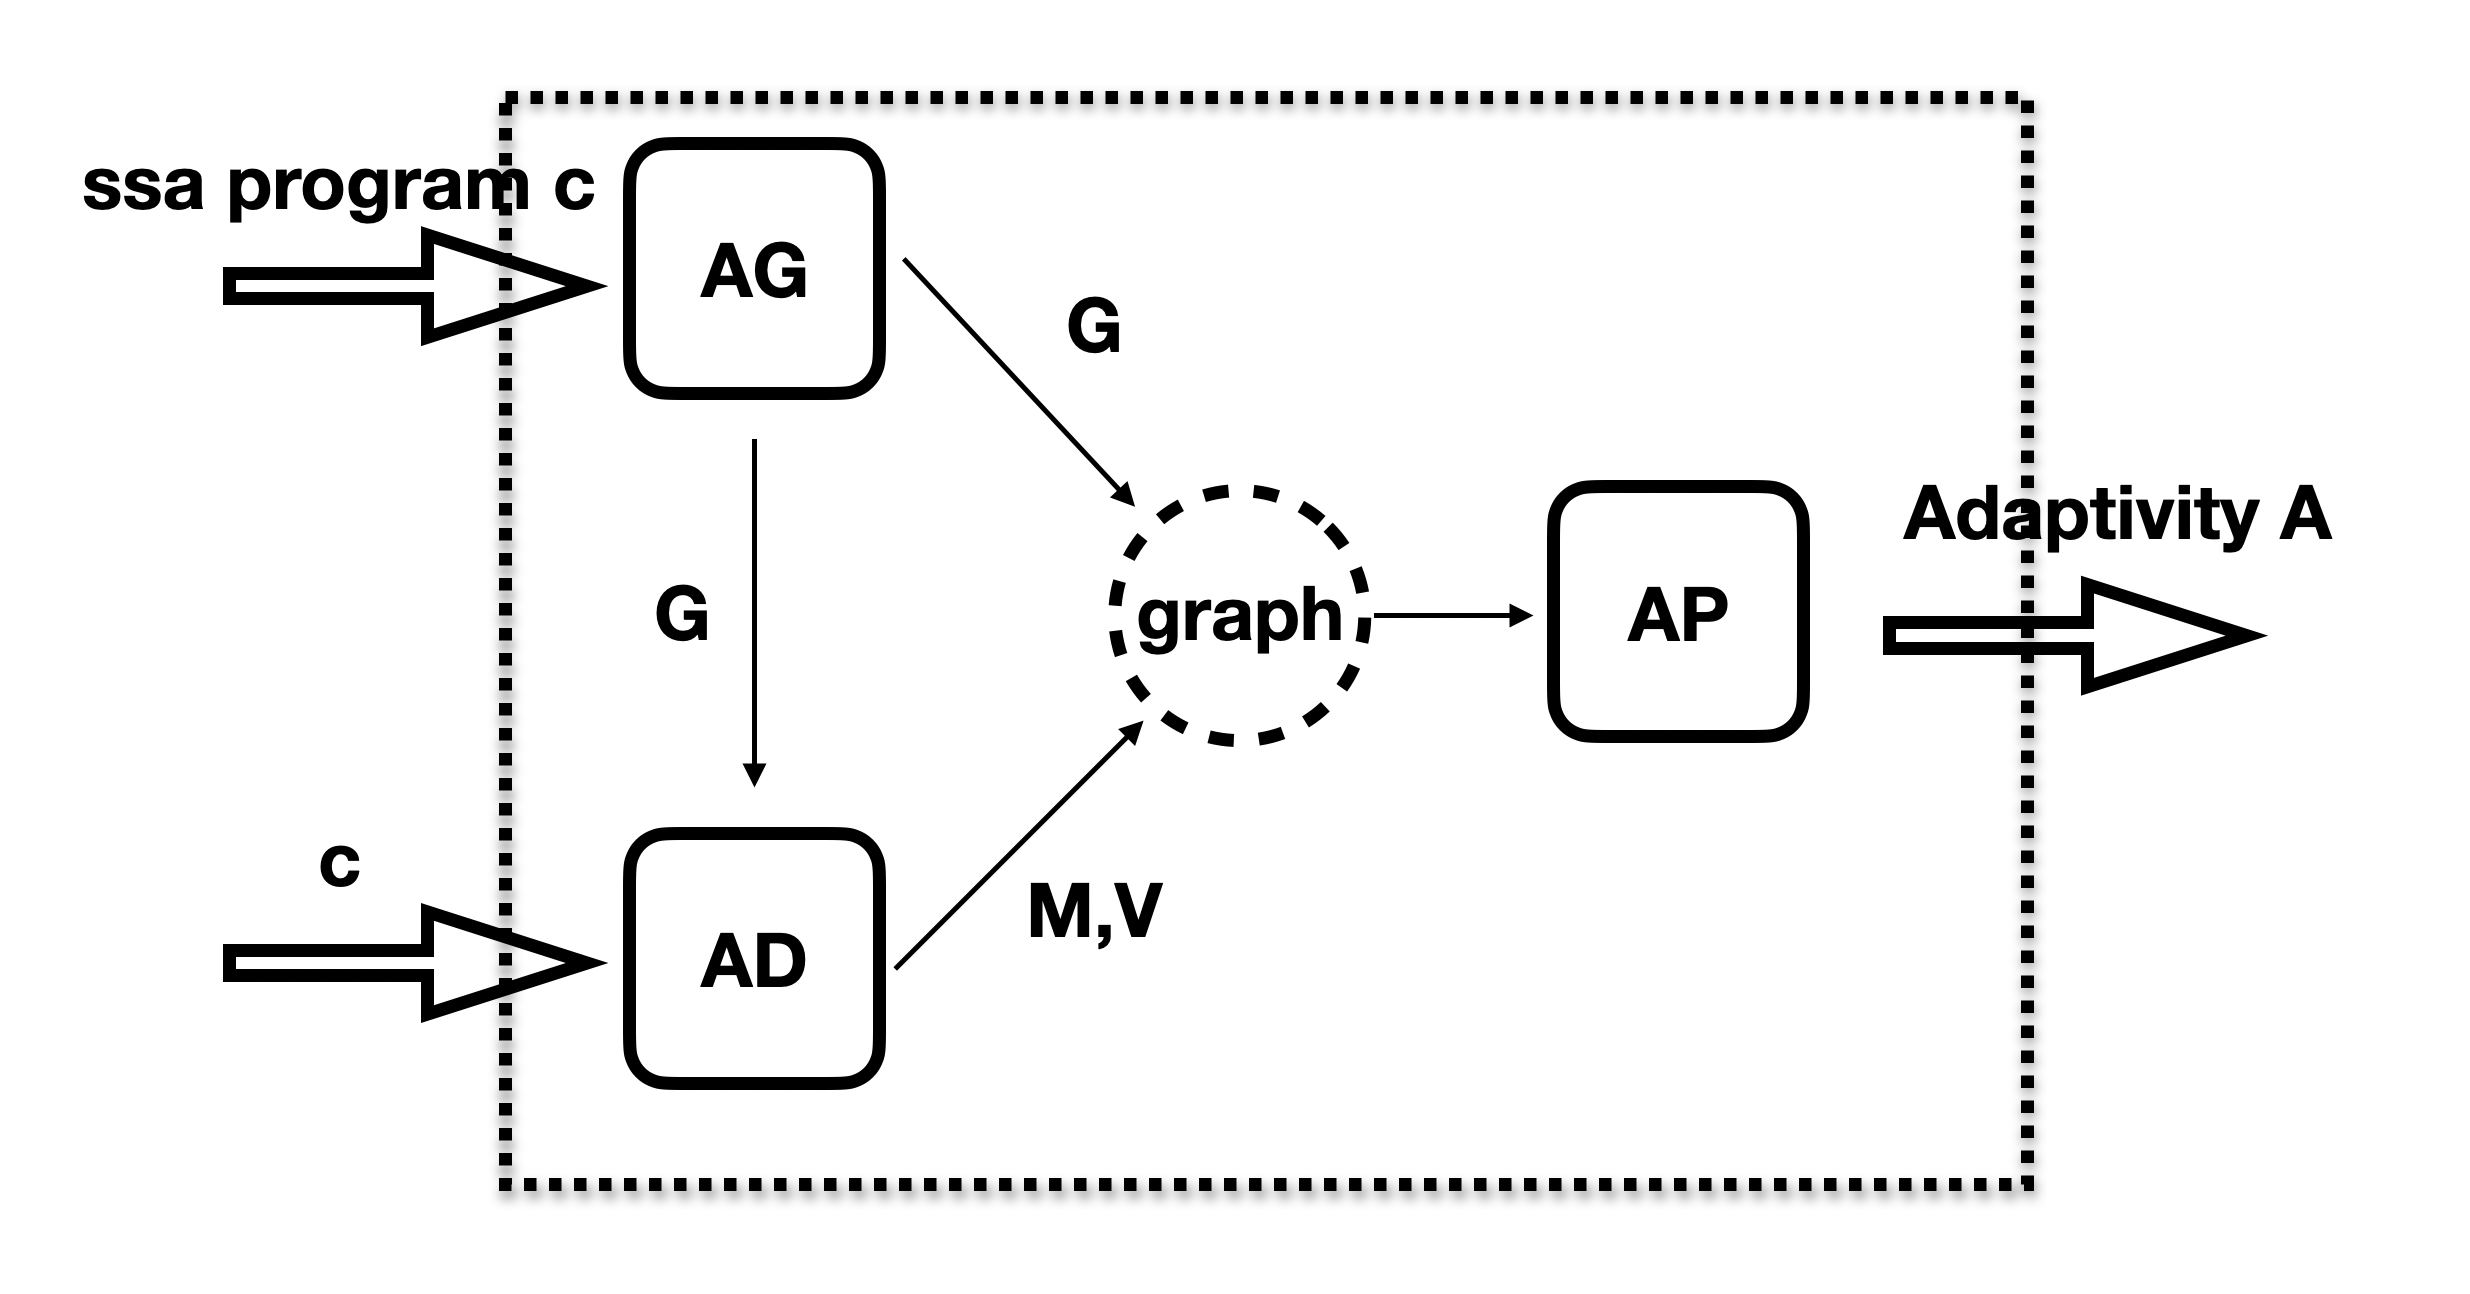
\includegraphics[width=1.0\columnwidth]{adapfun.png}
  \vspace{-0.3cm}
  \caption{The overview of {\THESYSTEM}}
  \label{fig:adaptfun}
  \vspace{-0.5cm}
\end{figure}
\subsubsection{Graph Estimation}
%
%
% \subsection{A guide to the algorithm}
% In order to have the upper bound of adaptivity:
% \\
% \begin{enumerate}
% \item $\THESYSTEM$  first builds a program-based dependency graph to {over-}approximate the
% % execution-based dependency graph (in Definition~\ref{def:trace_graph})
% Execution-Based Dependency Graph (in Definition~\ref{def:trace_graph})
% through Section~\ref{sec:alg_vertexgen}, Section~\ref{sec:alg_weightedgegen} and~\ref{sec:alg_graphgen}:
% % in the phases one to phases four of $\THESYSTEM$ in Section~\ref{sec:abscfg} to Section~\ref{sec:alg_graphgen}:
% \\
% 1.1 approximate the vertices: 
% % in the forth step of
% in the first phase of $\THESYSTEM$ in
% % the algorithm in Section~\ref{sec:alg_graphgen} 
% Section~\ref{sec:alg_vertexgen}
% without extra static analysis technique.
% \\
% 1.1 approximate the query annotations: 
% % in the forth step of
% in the first phase of $\THESYSTEM$ in
% % the algorithm in Section~\ref{sec:alg_graphgen} 
% Section~\ref{sec:alg_vertexgen}
% without extra static analysis technique.
% \\
% 1.2 approximate the vertices weights:
% in the second phase of 
% % the algorithm in  
% of $\THESYSTEM$ specifically in Section~\ref{sec:alg_weightgen}
% \\
% 1.3 approximate the edges between vertices:
% also in the second phase of $\THESYSTEM$ specifically in 
% % Section~\ref{sec:alg_weightgen}
% Section~\ref{sec:alg_edgegen}
% \\
% 1.4 generate the final approximated program-based dependency graph in Section~\ref{sec:alg_graphgen}
% %  to {over-}approximate the
% % approximate the query annotation: 
% % in the forth step of
% in the third phase of $\THESYSTEM$.
% % the algorithm  without extra static analysis technique.
% % \\
% This program-based graph has a similar topology structure as 
% % the one
% % of 
% the Execution-Based Dependency Graph. It has the same
% vertices and query annotations, but approximated edges and weights. 
% \item Then in the last phase in Section~\ref{sec:alg_adaptcompute}, $\THESYSTEM$
% % we compute the upper bound for adaptivity over this approximated graph:
% % , as an upper bound for
% % program's adaptivity
% computes the upper bound for adaptivity over this approximated graph.
% % in the last phase of this algorithm in Section~\ref{sec:alg_adaptcompute}.
% % \subsection{Adaptivity Based on Program Analysis in \THESYSTEM}
% % In order to give a bound on the program's adaptivity, we first build a
% % program-based data-dependency graph to {over-}approximate the
% % trace-based dependency graph.  Then, we define a program-based
% % adaptivity over this approximated graph, as an upper bound for
% % $A(c)$.
% \end{enumerate}
According to the dependency graph we use in adaptivity definition, we want to build a similar graph to {over-}approximate the
% execution-based dependency graph (in Definition~\ref{def:trace_graph})
Execution-Based Dependency Graph (in Definition~\ref{def:trace_graph}). The construction considers the vertices, edges, and the weight of every node, as well as some annotations which marks the query usage. The overall picture of this step is organized as follows.
% through Section~\ref{sec:alg_vertexgen}, Section~\ref{sec:alg_weightedgegen} and~\ref{sec:alg_graphgen}:


\begin{enumerate}
\item  Vertices are the assigned variables with unique labels, which is extracted directly from the program, see Section~\ref{sec:alg_vertexgen}
without extra static analysis technique
% \item Query annotations are also decided directly from the program, when there is a query request, the associated variables which are the results of the query requests are marked in the form of a flag, $0$ means no query, $1$ represents query related. See Section~\ref{sec:alg_vertexgen}.
\item The edge between vertices considers both control flow and data flow, See
Section~\ref{sec:alg_edgegen}
\item Every vertex and edge come with a weight, which tells the maximal times each vertex and edge can be visited in realistic execution. This weight is estimated by a reachability bound analysis on each vertex, See Section~\ref{sec:alg_weightgen}.
% \item Each edge also vertices considers both control flow and data flow, See
% Section~\ref{sec:alg_edgegen}
\item  Finally, with all the ingredients ready, we construct the final approximated program-based dependency graph in Section~\ref{sec:alg_graphgen}
\end{enumerate}

% the algorithm  without extra static analysis technique.
% \\
Overall, this program-based graph has a similar topology structure as 
% the one
% of 
the Execution-Based Dependency Graph. It has the same
vertices and query annotations, but approximated edges and weights. We call the graph generated by static analysis techniques, static analysis dedendency graph. 
% \item Then in the last phase in Section~\ref{sec:alg_adaptcompute}, $\THESYSTEM$
% % we compute the upper bound for adaptivity over this approximated graph:
% % , as an upper bound for
% % program's adaptivity
% computes the upper bound for adaptivity over this approximated graph.
% in the last phase of this algorithm in Section~\ref{sec:alg_adaptcompute}.
% \subsection{Adaptivity Based on Program Analysis in \THESYSTEM}
% In order to give a bound on the program's adaptivity, we first build a
% program-based data-dependency graph to {over-}approximate the
% trace-based dependency graph.  Then, we define a program-based
% adaptivity over this approximated graph, as an upper bound for
% $A(c)$.


\subsubsection{Adaptivity Computation}

Likewise the adaptivity is defined as a finite walk in the execution based depdenency graph, our static estimation on this adaptivity also relies on finding a path in the static analysis depdenency graph.   The construction of the stastic analysis dependency graph is of great value of showing some useful properties of the target program, such as dependency between variables, the execution upper bound of a certian command, while the key novelty is our path searching algorithm, which connects all the information we need in the static anlaysis dependency graph and provides us a sound over-estimation of adaptivity! In order to get a sound but precise upper bound, we will discuss some challenges in finding the 'appropriate' path in the graph, and how our algorithm responds to these challengs. We present the path seaching algorithm in Section~\ref{sec:alg_adaptcompute}.
 
% An
% approximated edge correspond to a program-based data dependency
% relation ($\flowsto$ in Definition~\ref{def:flowsto}) and an approximated
% weight corresponds to a reachability bound analysis results from
% Definition~\ref{def:transition_closure}.

% %
% \subsubsection{Program-Based Variable Dependency}
% The program-based dependency relation over two labeled variables ($x^i, y^j)$ is defined as a $\flowsto$ relation with respect to the program $c$ as follows.
% %
% \begin{defn}[Data Flow Relation between Assigned Variables ($\flowsto$)].
% \label{def:flowsto}
% \\
% Given a program  ${c}$,
% a variable ${x^i}  \in \lvar_c $ is in the \emph{flows to} relation with another variable ${y^j} \in \lvar_c$, if and only if:
% \mg{I cannot even parse the next formula. Why there is a big disjunction on the left? Disjunction is a binary operation, or n-ary if given a set, what is this disjunction between?}\\
% \mg{please, remove the underscript $c$ in the exists. It just makes everything mroe difficult to parse.}\\
% \mg{The use of $\lor$ is odd. E.g. $\exists {(\expr \lor \qexpr)}$ or
%   $ [{\assign{y}{\expr \lor \query(\qexpr)}}]^{j} $. I suggest to write the whole formula instead of using weird shortenings.}\\
% \mg{Also, now it is too late to change this but instead of breaking down the definition using the subterm relation and then defining the flowto relation, it would have been better to give just one inductive definition of Flowto - I imagine that this makes also the proof more awkward.}
% %
% {\footnotesize 
% \[
% \begin{array}{l}
% \flowsto({x^i, y^j, c}) \triangleq 
% \\
% \left( \bigvee
% \begin{array}{l}
% (\exists \expr \st \clabel{\assign{y}{\expr}}^j \in_{c} {c} 
% \land {x} \in FV(\expr) \land (x^i \in \live(j, c)))
% \\
% (\exists {\qexpr} \st [\assign{y}{\query({\qexpr})}]^j \in_{c} {c} 
% \land x \in FV({\qexpr}) \land (x^i \in \live(j,c))))
% \\
% \Big(\exists {c_w} \in \cdom, l \in \mathcal{L}, \bexpr \st
% 	\ewhile [\bexpr]^l \edo {c_w} \in_{c} {c}
% 	\land \flowsto(x^i, y^j, c_w)
% 	\\ \qquad	
%      \lor 
% 	\big( \exists {(\expr \lor \qexpr)} \st
% 	[{\assign{y}{\expr \lor \query(\qexpr)}}]^{j} \in_{c}  {c_w}  \land {x} \in FV(\bexpr) \land x^i \in \live(l, c)
% 	\big)
% 	\Big)
% \\
% \Big(
% \exists {c_1}, {c_2} \in \cdom, l \in \mathcal{L}, \bexpr 
% \st 
% 	\eif([\bexpr]^l, {c_1}, {c_2}) \in_{c} {c} \land
% 	\flowsto(x^i, y^j, c_1) \lor \flowsto(x^i, y^j, c_2)
% 	\\ \qquad 
% 	\lor 
% 	\big( \exists {(\expr \lor \qexpr)} \st
% 	\land {x} \in FV(\bexpr) \land x^i \in \live(l, c) \land
% 	([{\assign{y}{\expr \lor \query(\qexpr)}}]^{j} \in_{c}  {c_1}  
% 	\lor [{\assign{y}{\expr \lor \query(\qexpr)}}]^{j} \in_{c}  {c_2})
% 	\big)
% \Big)
% % \\
% \end{array}
% \right).
% \end{array}
% \]
% }
% %
% \end{defn}
% %
% \mg{The next notation is inconsistent with the one used above. Also, this definition should be given before the definition of flowto. From the description I have no cluse what this notion of reachability means. Also, the definition is referred to does not define this notation.}\\
% \mg{the definition somehow seems to make sense but until when the or notation is fixed and I don't see the definition of RD, I cannot tell for sure.}
% $\live^l(c) \subseteq \lvar_c$,
% which is the set of all the reachable variables at location of label $l$ in the program $c$.
% For every labelled variable $x^l$ in this set, 
% the value assigned to that variable
% in the assignment command associated to that label is reachable at the entry point of  executing the command of label $l$.
% This is formally defined , formally computed in Definition~\ref{def:feasible_flowsto}
% \\
% \mg{This description seems inconsistent with the definition. I suggest to use the same variables and terms.}
% To understand the $\flowsto$ intuition, 
% given a program  ${c}$ with its labelled variables $\lvar_c$, and two variables ${x^i}, y^j  \in \lvar_c $ 
% % showing up as $i$-th, $j$-th elements in $\lvar$ 
% % (i.e., ${x} = \lvar(i)$ and ${y} = \lvar(j)$),
% we say $y^j$ flows to ${x^i}$ in ${c}$ if and only if 
% the value of $y^j$ directly or indirectly influence the evaluation of the value of ${x}$ as follows:
% %
% \begin{itemize}
% \item (Explicit Influence) The program ${c}$ contains either 
% a command $[\assign{{x}}{\aexpr}]^i$ or $[\assign{{x}}{\query({\qexpr})}]^i$,
% such that ${y}$ shows up as a free variable in $\expr$ or ${\qexpr}$.
% We use $\flowsto({x^i, y^j, c})$ to denote $y^j$ flows to $x^i$ in ${c}$.
% %
% \item (Implicit Influence) The program ${c}$ contains either a while loop
% command
% or if command, 
% such that $x$ shows up in the guard
% and $y$ shows up in the left hand of an assignment command and this assignment command showing up
%  in the body of the while loop, or branches of if command.
% \end{itemize}
% %
% % This is formally defined in \ref{def:flowsto}.
% % We use $FV(\expr)$, $FV(\sbexpr)$ and $FV(\qexpr)$ denote the set of free variables in 
% % expression $\expr$, boolean expression $\sbexpr$ and query expression $\qexpr$ respectively.
% %
% %
% \mg{I don't understand what this definition of equivalence means. It is not observational equivalence
% and it is not syntactic equivalence. What are we trying to capture here? Also, it is equivalence of programs, not of program.}
% \begin{defn}[Equivalence of Program]
% %
% \label{def:aq_prog}
% Given 2 programs $c_1$ and $c_2$:
% \[
% c_1 =_{c} c_2
% \triangleq 
% \left\{
%   \begin{array}{ll} 
%     \etrue        
%     & c_1 = \eskip \land c_2 = \eskip
%     \\ 
%     \forall \trace \in \mathcal{T} \st \exists v \in \mathcal{VAL}
%     \st \config{ \trace, \expr_1} \aarrow v \land \config{ \trace, \expr_1} \aarrow v     
%     & c_1 = \assign{x}{\expr_1} \land c_2 = \assign{x}{\expr_2} 
%     \\ 
%     \qexpr_1 =_{q} \qexpr_2       
%     & c_1 = \assign{x}{\query(\qexpr_1)} \land c_1 = \assign{x}{\query(\qexpr_2)} 
%     \\
%     c_1^f =_{c} c_2^f \land c_1^t =_{c} c_2^t
%     & c_1 = \eif(b, c_1^t, c_1^f) \land c_2 = \eif(b, c_2^t, c_2^f)
%     \\ 
%     c_1' =_{c} c_2'         
%     & c_1 = \ewhile b \edo c_1' \land c_2 = \ewhile b \edo c_2'
%     \\ 
%     c_1^h =_{c} c_2^h \land c_1^t =_{c} c_2^t
%     & c_1 = c_1^h;c_1^t \land c_2 = c_2^h;c_2^t 
%   \end{array}
%   \right.
% \]
% %
% As usual, we denote by $c_1 \neq_{c} c_2$ the negation of the equivalence.
% %
% \end{defn}
% %
% \mg{This definition needs to go before it is used. }
% Given 2 programs $c$ and $c'$, we denote by $c' \in_{c} c$  that $c'$ is a sub-program of $c$ defined as follows,
% \begin{equation}
% c' \in_{c} c \triangleq \exists c_1, c_2, c''. ~ s.t.,~
% c =_{c} c_1; c''; c_2 \land c' =_{c} c''
% \end{equation} 
% %

% \subsubsection{Program Analysis Based Dependency Graph}
% We give the formal definition for the program-based dependency graph for a program $c$, 
% $\progG({c}) = (\vertxs, \edges, \weights, \flag)$ as follows.
% \begin{defn}
%     [Program-Based Dependency Graph].
%     \label{def:prog_graph}
%     \\
% Given a program ${c}$
% its program-based graph 
% $\progG({c}) = (\vertxs, \edges, \weights, \qflag)$ is defined as:
% {\footnotesize
% \[
% \begin{array}{rlcl}
% \text{Vertices} &
% \vertxs & := & \left\{ 
% x^l \in \mathcal{LV} 
% ~ \middle\vert ~
% x^l \in \lvar_{c}
% \right\}
% \\
% \text{Directed Edges} &
% \edges & := & 
% \left\{ 
%   ({x}_1^{i}, {x}_2^{j}) \in \mathcal{LV} \times \mathcal{LV}
%   ~ \middle\vert ~
%   \begin{array}{l}
%     {x}_1^{i}, {x}_2^{j} \in \vertxs
% 	\land
%     % \\
%     \exists n \in \mathbb{N}, z_1^{r_1}, \cdots, z_n^{r_n} \in \lvar_{{c}} \st 
%     n \geq 0 \land
%     \\
%     \flowsto(x^i,  z_1^{r_1}, c) 
%     \land \cdots \land \flowsto(z_n^{r_n}, y^j, c) 
%   \end{array}
% \right\}
% \\
% \text{Weights} &
% \weights & := &
% % \bigcup
% % \begin{array}{l}
% 	\left\{ (x^l, w) \in  \mathcal{LV} \times EXPR(\constdom)
% 	\mid
% 	x^l \in \lvar_{{c}} \land w = \absW(l)
% 	\right\}
% % \end{array} 
% \\
% \text{Query Annotation} &
% \qflag & := & 
% \left\{(x^l, n)  \in  \mathcal{LV} \times \{0, 1\} 
% ~ \middle\vert ~
%  x^l \in \lvar_{c},
% n = 1 \iff x^l \in \qvar_{c} \land n = 0 \iff  x^l \in \qvar_{c} .
% \right\}
% \end{array}
% \] 
% }
% , where the $\absW(l)$ is the symbolic reachability bound in domain of $EXPR(\constdom)$,
% % for the assignment command of label $l$ to which  
% the labeled variable $x^l$, 
% % is associated, 
% computed from the $\THESYSTEM$ algorithm 
% in Definition~\ref{def:transition_closure}.
% The $EXPR(\constdom)$ is an expression over symbolic constants containing the
% input variables and natural number.
% \end{defn} 
% %
% \paragraph{Program-Based Adaptivity ($\progA(c)$)}
% %
% Given a program ${c}$, we generate its program-based graph 
% $\progG({c}) = (\vertxs, \edges, \weights, \qflag)$.
% %
% Then the adaptivity bound based on program analysis for ${c}$ 
% % is the number of query vertices on a finite walk in $\progG({c})$. This finite walk satisfies:
% % \begin{itemize}
% % \item the number of query vertices on this walk is maximum
% % \item the visiting times of each vertex $v$ on this walk is bound by its reachability bound $\weights(v)$.
% % \end{itemize}
% is computed as the maximum query length over all finite walks in $\walks(\progG({c}))$,
% %
% % It is formally defined in \ref{def:prog_adapt}.
% defined formally as follows.
% %
% %
% \begin{defn}
% [{Program-Based Adaptivity}].
% \label{def:prog_adapt}
% \\
% {
% Given a program ${c}$ and its program-based graph 
% $\progG({c}) = (\vertxs, \edges, \weights, \qflag)$,
% %
% the program-based adaptivity for $c$ is defined as%
% \[
% \progA({c}) 
% := \max
% \left\{ \qlen(k)\ \mid \  k\in \walks(\progG({c}))\right \}.
% \]
% }
% \end{defn}  
%
%
% {
% \begin{defn}[Variable Flags ($\flag$)].
% \\
% Given a program  ${c}$ with its labelled variables $\lvar$, the $\flag$ is a vector of the same length as $\lvar$, s.t. for each variable ${x}$ showing up as the $i$-th element in $\lvar$ (i.e., ${x} = \lvar(i)$), 
% $\flag(i) \in \{0, 1, 2\}$ is defined as follows:
% %
% %
% \[
% \flag(i) := 
% \left\{
% \begin{array}{ll}
% 2 & 
% {x^l} \in \lvar_{c} \land 
% (\exists {\qexpr}. ~ s.t., ~
% [\assign{{x}}{\query({\qexpr})}]^l \in_{c} {c})
% \\
% 1 &  
% \begin{array}{l}
% {x^l} \in \lvar_{c} \bigwedge \\
% \left(
% \begin{array}{l}
% \big(\exists  ~ {c'}, {\expr}, \sbexpr, l, l'. ~
% 	\ewhile [\sbexpr]^l \edo {c'} \in_{c} {c}
% 	\land 
% 	[{\assign{x}{\expr}}]^{l'} \in_{c}  {c'}
% \big) \bigvee
% \\
% \big(\exists ~ \sbexpr, l, l_1, l_2, {c_1}, {c_2}, {\expr}_1, {\expr}_2. ~
% 	\eif([\sbexpr]^l, {c_1}, {c_2}) \in_{c} {c} \land
% 	([{\assign{x}{\expr_1}}]^{l1} \in_{c} {c_1} \lor 
% 	[{\assign{x}{\expr_2}}]^{l2} \in_{c} {c_2})
% \big)
% \end{array}
% \right)
% \end{array}
% \\
% 0 & \text{o.w.}
% \end{array}
% \right\}. 
% \] 
% %
% \end{defn}
%
% Operations on $\flag$ are defined as follows:
% \begin{equation}
% \begin{array}{llll}
% {\flag_1 \uplus \flag_2}(i) & := &
% \left\{
% \begin{array}{ll}
% k & k = \max{\big\{\flag_1(i), \flag_2(i)\big\}} 
% \land |\flag_1| = |\flag_2|\\
% 0 & o.w.
% \end{array}\right.
% & i = 1, \cdots, |\flag_1|  
% \\
% {\flag \uplus n}(i) & := & 
% \max\big\{ \flag(i), n \big\} 
% & i = 1, \ldots, |\flag|    
% \\
% \left[ n \right]^k (i) & := &  n
% & i = 1, \ldots, k ~ \land ~ |\left[ n \right]^k| = k
% \end{array}
% \end{equation}
%
%
%
% \begin{defn}[Data Flow Matrix ($\Mtrix$)]
% The data flow matrix $\Mtrix$ of a program $c$ is a matrix of size $|\lvar_c| \times |\lvar_c|$ 
% s.t.,
% %
% \[
% \Mtrix(i, j) \triangleq
% \left\{
% \begin{array}{ll}
% 1	&	\flowsto({x^i, y^j, c}) \\
% 0	& o.w.
% \end{array}
% \right., {x^i}, y^j  \in \lvar_c.
% \]
% %
% \end{defn}
% %
% Operations on the data flow matrices are defined as follows:
% %
% \begin{equation}
% \Mtrix_1 ; \Mtrix_2 
% := \Mtrix_2 \cdot \Mtrix_1 + \Mtrix_1 + \Mtrix_2
% \end{equation}
% %
% Consider the same program $c$ as above, its data flow matrix $\Mtrix$ and $\flag$ for the program $c$ is as follows:
% $$
% {c} = 
% \begin{array}{l}
% \left[{\assign {x_1} {\query(0)}}	\right]^1;
% \\
% \left[{\assign {x_2} {x_1 + 1}}		\right]^2;
% \\
% \left[{\assign {x_3} {x_2 + 2}}		\right]^3
% \end{array}
% ~~~~~~~~~~~~
% \Mtrix
% =  \left[ 
% \begin{matrix}
% 0 & 0 & 0 \\
% 1 & 0 & 0 \\
% 1 & 1 & 0 \\
% \end{matrix} \right] ~ , 
% \flag = \left [ \begin{matrix}
% 1 \\
% 0 \\
% 0 \\
% \end{matrix} \right ]
% $$
% %
% % There are two special matrices used for generating the data flow matrix $\Mtrix$ in the analysis algorithm. They are the left matrix $\lMtrix_i$ and right matrix $\mathsf{R_{(e, i)}}$.

% % Given a program  ${c}$ with its labelled variables $\lvar$ of length $N$,
% % the left matrix $\lMtrix_i$ generates a matrix of $1$ column, $N$ rows, 
% % where the $i$-th row is $1$ and all the other rows are $0$.
% % %
% % \begin{defn}[Left Matrix ($\lMtrix_i$)].
% % \\
% % Given a program  ${c}$ with its labelled variables $\lvar$ of size $N$, 
% % the left matrix $\lMtrix_i$ is defined as follows:
% % \[
% % \lMtrix_i(j) : = 
% % \left
% % \{
% % \begin{array}{ll}
% % 1 & j = i \\
% % 0 & o.w.
% % \end{array}
% % \right.,
% % j = 1, \ldots, N.
% % \]
% % \end{defn}
% % %
% % Given a program  ${c}$ with its labelled variables $\lvar$ of length $N$,
% % the right matrix $\rMtrix_{\expr, i}$ generates a matrix of one row and $N$ columns, 
% % where the locations of free variables in $\expr$ is marked as $1$. 
% % %
% % %
% % \begin{defn}[Right Matrix ($\rMtrix_{\expr}$)].
% % \\
% % Given a program  ${c}$ with its labelled variables $\lvar$ of length $N$, 
% % the right matrix $\rMtrix_{\expr}$ is defined as follows:
% % \[
% % \rMtrix_{\expr}(j) : = 
% % \left\{
% % \begin{array}{ll}
% % 1 & {x} \in FV(\expr) 
% % \\
% % 0 & o.w.
% % \end{array}
% % \right.,
% % {x} = \lvar(j) ~ , ~ j = 1, \ldots, N.
% % \]
% % %
% % %
% % \end{defn}
% % %
% % Using the same example program ${c}$ as above with labelled variables $\lvar = [ {x_1 , x_2 , x_3} ] $,
% % the left and right matrices w.r.t. its $2$-nd command 
% % $\left[{\assign {x_2} {x_1 + 1}}\right]^2$  are as follows:
% % \[
% % \lMtrix_1 = \left[ \begin{matrix}
% % 0   \\
% % 1 	 \\
% % 0   \\
% % \end{matrix}   \right ] 
% % ~~~~~~~~~~~~~~
% % \rMtrix_{{x}_1 + 1}
% % = \left[ \begin{matrix} 
% % 1 & 0 & 0 \\
% % \end{matrix}  \right]
% % \]
% %
% %
% %
% \subsection{ $\THESYSTEM$ Analysis Algorithm}
% \subsection{Dependency Graph Estimation}
\subsection{Vertices Estimationn}
\label{sec:alg_vertexgen}
The first component of every vertex in the static analysis dependency graph are actually identical as the  Execution-Based Dependency Graph, which are assigned variables in the program annotated with the unique label(line number). 
These vertices are collected by statically scanning the program, like what we do for vertices of its Execution-Based Dependency Graph. 
The vertices are defined formally as follows.

  \highlight{
\[
    \progV^0(c) \triangleq \left\{ 
  (x^l, w) \in \mathcal{LV} \times \mathcal{A}_{\lin}
  ~ \middle\vert ~
  x^l \in \lvar(c)
  \right\}
  \]
  }
  %
where $\mathcal{A}_{\lin}$ is the set of arithmetic expressions over $\mathbb{N}$ and program's input variables. 
The weight $w$ for every vertex will be computed in following step in Section~\ref{sec:alg_weightgen}.
% The static scanning of the programs also tells us whether one vertice(assigned variable) is assigned by a query request. We have similar definition when defining the Execution-Based Dependency Graph, 
% a set of pairs $\progF(c) \in \mathcal{P}(\mathcal{LV} \times \{0, 1\} )$ 
% % is the set of pairs 
% % The weight for each vertex in $\progV(c)$ is computed 
% mapping each $x^l \in \progV(c)$ to a flag, either $0$ or $1$, where $1$  means $x^{l}$ is a member of $ \qvar_{c}$, a set of those variables assigned with query requests, and $0$ means $x^{l}$ not in this set. It is defined formally below.

% \[\progF(c) =\left\{(x^l, n)  \in  \mathcal{LV} \times \{0, 1\} 
% ~ \middle\vert ~
% x^l \in \lvar_{c},
% n = 1 \iff x^l \in \qvar_{c} \land n = 0 \iff  x^l \not\in \qvar_{c} .
% \right\}\]
%

% \wq{To do: Add $\THESYSTEM$, a data flow analysis algorithm to scan the program and give a graph.}
% {\THESYSTEM} consists of three phases: 
% \begin{enumerate}
%     \item Generating an abstract control flow graph with each edge representing an abstract event transiting between two command labels. 
%     \item Computing the value bound invariant for each variable in the event and 
%     the event transition closure over the abstract control flow graph,
%     we get the reachability bound for each labeled command.
%     \item Refining the abstract control flow graph with data-flow, by performing the reaching definition analysis, we generate a weighted data control flow graph.
%     \item An algorithm to find the appropriate path in the weighted data control flow graph
% \end{enumerate}

% \begin{enumerate}
%     \item An algorithm to generate a precise data control flow graph
%     \item An algorithm to perform a Reachability number analysis to calculate the weight of each node in the graph generated in phase 1.
%     \item An algorithm to find the appropriate path in the weighted data control flow graph
% \end{enumerate}

\subsection{Edge and Weight Estimation}
\label{sec:alg_weightedgegen}

Since the edges of the execution-based graph of a program relies on the dependency relation, which handles both control flow and data flow, as an over-approximation of this graph, the edges of our static anlaysis dependency graph also covers these two kind of flows. We develop a feasible data flow relation to catch these two flows, in Section~\ref{sec:alg_edgegen}.


The weight of every vertice in the execution-based graph is built on all possible execution traces.
In order to over-approximate the weight statically but still tightly, we present a symbolic reachability bound analysis for estimation of the weight of each vertice(label) in Section~\ref{sec:alg_weightgen},
in spirit of some reachablility bound techiniques.


The edges and weight estimation are both performed on basis of an abstract control flow graph of the program, we first show how to generate this abstract execution control flow graph before the introduction of  the edge and weight estimation.  

% This analysis first 
%  generate an abstract control flow graph
%  over all program labels, 
% in order to analyzing the data flow relations through variables assigned in every labeled command,
% and the reaching time of each variable.
% Then, it refines this control flow graph 
% % into a weighted data-dependency graph, 
% and generate the Program-Based Dependency Graph,
% through the data flow and reaching bound analysis results.
% In the last step, it finds the longest finite walk in this weighted data control flow graph w.r.t. the query variables,
% and return the number of query vertices traversed alongside.
% % \wq{To do: Add $\THESYSTEM$, a data flow analysis algorithm to scan the program and give a graph.}
% To be more specific, {\THESYSTEM} consists of five phases as follows,
% \\
% % \jl{Better to have a graph or picture of overview of the algorithm}
% \todo{graph}
% \todo{pass again}
% This analysis
% \begin{enumerate}
%     % \item Generating 
%     \item first generate 
%     an abstract control flow graph
%     %  over all labels,
%     (remove?? with program's labels as vertices and abstract transitions as edges)
%     in Section~\ref{sec:abscfg},
%     % used to analyze 
%     for analyzing the weight of every vertex in $\progV(c)$ and edges between every vertex in $\progV(c)$ in the next two steps;
%     %  \ref{sec:alg_weightgen} and 
%     % \ref{sec:alg_edgegen}.

%     % which are used as program's control locations,
%     %
%     \item then use the abstract control flow graph generated above, 
%     compute the weight of every vertex in $\progV(c)$ by computing a symbolic reachability bound for each label in Section~\ref{sec:alg_weightgen},
%     % \\
%     \item and then use the same graph again to estimate the edges between every vertex in $\progV(c)$ by computing the feasible data flow relation between every labeled variables in Section~\ref{sec:alg_edgegen}.
  
% \end{enumerate}

\subsubsection{Abstract Execution Control Flow graph}
\label{sec:abscfg}
% In an 
%  % a program $c$ 
%  abstract control flow graph for a program $c$, $\absG(c)$, 
%  every 
%  vertex corresponds to the unique
%  label.
%  Specifically,
%  The edge is directed, 
%   representing an abstract transition 
%   between two control locations uniquely decided by the labels.   
%    (We refer control location and the label to the same thing). The abstract transition is of the form of a set of difference constraints for variables, built from the abstract execution trace of the program. For instance, the edge $(l_1, dc, l_2)$ from $l_1$ to $l_2$,
%   represents an abstract transition 
%   between two control locations with a set of difference constraints on it.
%  In this transition, the  command labeled with the second location $l_2$, 
%   will be executed after execution of the command with label $l_1$,
%  %  The abstract transition contains a set of difference constraints for variables, 
%  with the difference constraints generated by abstracting the command of the first label. Difference constraints is a constraint on difference between variables and constants, which will be formally introduced when we discuss experssion abstraction.
%  \wq{The edge in the abstract control flow graph comes from the abstract execution trace of the program. The abstract execution trace, an abstract representation of the execution, consists of a list of abstract transitions. Then, every abstract transition in the abstrction execution trace corresponds to an edge in the abstract control flow graph. In aonther word, the edge $(l_1, dc, l_2)$ in the abstract control flow graph, represents an abstract transition 
%   from $l_1$ to $l_2$, with a set of difference constraints $dc$. Also notice, the difference constraints generated during the abstract transition appears in the edge as annotation.}

%  % over program's abstract execution 

%  Overall, the key point of the abstract excution control flow graph is the construction of the abstract execution trace of a program, which relies on a program abstraction procedure in following steps:

%  \begin{enumerate}
%  \item  Computing the abstract expression for every assignment command in the program.
%  \item Computing the abstract event for every labeled command in the program. Intuitively, this abstract event aims 
%  to approximate the event in program's execution trace.
%  \item Constructing the abstract execution trace for a program.
%  \end{enumerate}  

We discuss the vertices and edge of the
abstract control flow graph for a program $c$, $\absG(c)$.

Every 
vertex corresponds to the unique
label.
Specifically,
the vertices of this graph is the set of $c$'s labels with an exit label $l_{ex}$, 
\[ 
  \absV(c) = labels(c)\cup\{l_{ex}\}
  \]
%  corresponding to a label command in the program.

% \wq{
  The edge in the abstract control flow graph comes from the abstract execution trace of the program. 
  The abstract execution trace, an abstract representation of the execution, consists of a list of abstract transitions. 
  Then, every abstract transition in the abstraction execution trace corresponds to an edge in the abstract control flow graph. In another word, the edge $(l_1, dc, l_2)$ in the abstract control flow graph, represents an abstract transition 
 from $l_1$ to $l_2$, with a set of difference constraints $dc$. 
 Also notice, the difference constraints generated during the abstract transition appears in the edge as annotation.
%  }

% over program's abstract execution 


% \wq{
  Overall, the vertices can be easily collected and the key point of construction of the abstract execution control flow graph for a program is the abstract execution trace, 
  which relies on the abstraction of expression and abstract transition (we also call it abstract event), we will discuss in the following section.
   To make it easy to understand, abstract control flow graph is a control flow graph, with difference constraints on every edge.
  % }  

%
\paragraph*{Expression Abstraction}

The expression assigned to the variable on the left hand of the assignment command is abstracted to an abstract value: (adopted from the expression abstraction method in paper \cite{sinn2017complexity}). The abstract value is expressed in the form of Difference constraint, denotated as $DC : \mathcal{VAR} \cup \constdom \to \mathcal{\mathcal{VAR} \times (\mathcal{VAR} \cup \constdom) } \times (\mathbb{Z} \cup \{\infty\})$.  $\constdom$ is called the Symbolic Constant defined as $\constdom \triangleq \mathbb{N} \cup \inpvar \cup \{\max{(\dbdom)}\} $, which consists of 
natural numbers $\mathbb{N}$,
the program's input variables $\inpvar$  
and a constant value $Q_m$ for estimating the upper bound of variables which are
assigned by queries. 

Give an instance of difference constraint used here,
$DC(\mathcal{VAR}  \cup \constdom) \cup \{\top\}$ represents all the difference constraints over 
variable and symbolic constants. 
% The difference constraint $DC$ over $\mathcal{VAR} \cup \constdom$ 
It is a set of the inequality of form $x \leq y + v$ where $x \in \mathcal{VAR} $, 
$y \in \mathcal{VAR}  \cup \constdom$ and $v \in \mathbb{Z}$. 
This difference constraint is defined in the same way as
\cite{sinn2017complexity}. For concise, we use $\dcdom^{\top}$ to represent the $DC(\mathcal{VAR}  \cup \constdom) \cup \{\top\}$ .


We show the expression abstraction $\absexpr : \expr \to \mathcal{VAR} \to DC(\mathcal{VAR}  \cup \constdom) \cup \{\top\} $ below.

% We introduce the following notations and operations first
% % an expression abstraction method based on the expression abstraction in paper \cite{sinn2017complexity}.
% \\
% % is enriched into $\constdom \triangleq \mathbb{N} \cup \inpvar \cup \{\max{(\dbdom)}\} $.
% T
% \\

% represents the set of inequality over all $\mathcal{VAR}  \cup \constdom$. 

% The symbolic constant is enriched into $\constdom \triangleq \mathbb{N} \cup \inpvar \cup \{\max{(\dbdom)}\} $.
% It consists of 
% natural number $\mathbb{N}$,
% the symbolic constants $\inpvar$ (i.e., the set of the program's input variables), 
% and a constant value $Q_m$ for estimating the upper bound of variables which are
% assigned by queries.
% \\
% The symbolic constant is enriched into $\constdom \triangleq \mathbb{N} \cup \inpvar \cup \{\max{(\dbdom)}\} $.
% \\

% % $ \absdom: \mathcal{P}(DC(\mathcal{VAR}  \cup \constdom) \cup \{\top \})$:
% \\
% $\constdom: \mathbb{N} \cup \inpvar \cup \{\max{(\dbdom)}\} $ 
% The  constant 
% \\
% % $DC(\mathcal{VAR}  \cup \constdom)$ represents the set of inequality over all $\mathcal{VAR}  \cup \constdom$.
% \\

% \[
%   \begin{array}{ll} 
%     \absexpr(y + c, x)  = x' \leq y + c  & c \in \mathbb{N} \land y \in (VAR \cup \constdom) \\
%     \absexpr(y - c, x)  = x' \leq y - c  & c \in \mathbb{N} \land y \in (VAR \cup \constdom) \\
%     \absexpr(v, x)  = x' \leq v + 0  & v \in (VAR \cup \constdom) \\
%     \absexpr(\aexpr, x) = x' \leq 0 + \infty   & \aexpr \text{ doesn't have any of the forms as above} \\
%     \absexpr(\qexpr, x)  = x' \leq 0 + Q_m & \qexpr \text{ is a query expression}  \\
%     \absexpr(\bexpr, x) = x' \leq 0 + 1   & \bexpr \text{ is a boolean expression} \\
%   \end{array}
%   \]
  \[
    \begin{array}{ll} 
      \absexpr(x - v, x)  = x' \leq x - v  & x \in \grdvar \land v \in \mathbb{N} \\
      \absexpr(y + v, x)  = x' \leq y + v  & x \in \grdvar \land v \in \mathbb{Z} \land y \in (\grdvar \cup \constdom) \\
      \absexpr(v, x)  = x' \leq v + 0  & x \in \grdvar \land v \in (\grdvar \cup \constdom) \\
      \absexpr(y + v, x)  = x' \leq y + v & \\
      \grdvar = \grdvar \cup \{y\} & x \in \grdvar \land v \in \mathbb{Z} \land y \notin (\grdvar \cup \constdom)  \\
      \absexpr(\qexpr, x)  = x' \leq 0 + Q_m & x \in \grdvar \land \qexpr \text{ is a query expression}  \\
      \absexpr(\bexpr, x) = x' \leq 0 + 1   & x \in \grdvar \land \bexpr \text{ is a boolean expression} \\
      \absexpr(\expr, x) = x' \leq \infty  &  x \in \grdvar \land \expr \text{ doesn't have any of the forms as above} \\
      \absexpr(\expr, x) = \top  &  x \notin \grdvar \\
    \end{array}
    \]
  
  % \wq{ 
    $\grdvar$ is the set of variables used in the guard expression of every while command in the program $c$. 
  % }. 
  In the case 4, if a variable $x$, belonging to the set 
  $\grdvar$ is updated by a variable $y$, which isn't in this set, 
  we add $y$ into the set $\grdvar$ and repeat 
  above procedure  until $\grdvar$ and $\absexpr(\expr, x)$ is stabilized. 
  % \wq{I do not understand this sentence:-(}
  \\
Specifically 
% understanding the intuition, 
we handle a 
% simplified 
normalized guard expression ($ x > 0$ for $x^l \in \lvar_c$)
 in $\ewhile$, and 
%  \wq{I do not understand this sentence:-(}
%  .
% \\
% The counter variables only increase, decrease or reset by expression in the form of arithmetic minus and plus (able to extend to max and min.)
the counter variables only increase, decrease or reset by 
% expression in the form of 
simple arithmetic expression (mainly multiplication, division, minus and plus (able to extend to max and min)). 
This is the same as in paper \cite{sinn2017complexity}. 
\\
For more complex expression assignments, where the counter reset, or calculated from $\elog$, 
multiplication or division, and expressions involving multiple variables, the constraint is approximated as reset of $\infty$.
\\
% This simplification \wq{which part we simplify here?} 
This approximation strategy
doesn't affect our analysis results in our examples. It is easy to extend the normalized expression 
into more complex forms as in \cite{sinn2017complexity}, as well as the 
counter variable manipulation with more advanced expressions.
% \\ 
% The boolean expression in the guard of $\ewhile$ command is normalized into form of $ x > 0$ where $x^l \in \lvar_c$ for some $l$.


\paragraph{Program Event Abstraction}
We show the abstract event definition, which is generated when computing its abstract execution trace.

\begin{defn}[Abstract Event]
  \label{def:abs_event}
  Abstract Event: 
  $\absevent \in $
  $\ldom \times \dcdom^{\top} \times \ldom$
  is a 
  % pair of abstract initial state and final state.
  triple where the first and third components are labels,
  second component is a constraint from $\dcdom^{\top}$.
  % the thrid % computed from program's abstract final and initial state, $\absfinal(c)$ and $\absinit(c)$ with formal definition, and algorithm detail in Appendix.
  %  the constraint and the third corresponds to a final state.
  \end{defn}
  Specifically, in an abstract event, 
  the first label correspond to an initial state, and 
  the second label and the constraint correspond to an abstract final state.
 The abstract initial state is a label from $\ldom$.
The abstract final state is a pair from $\ldom \times \dcdom^{\top}$,  
where first component is a label from $\ldom$ and the second component is a constraint from $\dcdom^{\top}$.
%

%
Given a program $c$, its abstract initial state,
and the set of its abstract final state is computed as follows,
%
\[
  \begin{array}{ll}
    \absinit(\clabel{\assign{x}{\expr}}{}^l)  & = l  \\
    \absinit(\clabel{\assign{x}{\expr}}{}^l)  & = l \\
    \absinit(\clabel{\eskip}^{l})  & = l \\
    \absinit(\eif [b]^l \ethen c_1 \eelse c_2)  & = l \\
    \absinit(\ewhile [b]^l \edo c)  & = l \\
    \absinit(c_1 ; c_2)  & = \absinit(c_1) \\
 \end{array}
 \]
%
Final State Abstraction: 
$\absfinal: \cdom \to \mathcal{P}(\ldom \times \dcdom^{\top})$,
computes the set of Abstract Final State for the command. 
 \[
  \begin{array}{ll}
    \absfinal(\clabel{\assign{x}{\expr}}{}^l)  & = \{(l, \absexpr\eapp (\expr, x))\}  \\
     \absfinal(\clabel{\assign{x}{\query(\qexpr)}}{}^l)  & = \{
      (l, x' \leq 0 + Q_m )\}  \\
     \absfinal(\clabel{\eskip}^{l})  
     & = \{(l, \top)\} \\
     \absfinal(\eif [b]^l \ethen c_1 \eelse c_2)  & = \absfinal(c_1) \cup \absfinal(c_2) \\
     \absfinal(\ewhile [b]^l \edo c)  & = \{(l, \top)\} \\
     \absfinal(c_1 ; c_2)  & =  \absfinal(c_2) \\
 \end{array}
 \]
 %
 \paragraph{Abstract Execution Trace}
 Now, we  extract the abstract execution trace  $\absflow(c)$ for a program, which computes the Abstract Execution Trace for program $c$, as a set of the abstract events $\absevent$.
 %
 \begin{defn}[Abstract Execution Trace]
 \label{def:abs_trace}
  $\absflow \in \cdom \to \mathcal{P}( \ldom \times DC(\mathcal{VAR}  \cup \constdom) \cup \{\top\}) \times \ldom )$
  \end{defn}
 %

 
  We now show how to compute the abstract execution trace. 
  For simplicity, we use $\mathcal{P}(\absevent)$ represent the power set of all abstract events, and we have $\absflow(c) \in \mathcal{P}(\absevent)$.
 We first append a skip command with 
%  a symbolic label $l_e$, i.e., $\clabel{\eskip}^{l_e}$ at the end of the program $c$, and compute the $\absflow(c) = \absflow'(c')$ for $c'$, where $c' = c;\clabel{\eskip}^{l_e}$ as follows,
the exist label $l_{ex}$, i.e., $\clabel{\eskip}^{l_{ex}}$ at the end of the program $c$, 
and compute the $\absflow(c) = \absflow'(c')$ for $c'$, where $c' = c;\clabel{\eskip}^{l_{ex}}$ as follows,
 %
 {\footnotesize
 \[
   \begin{array}{ll}
      \absflow'(\clabel{\assign{x}{\expr}}{}^l)  & = \emptyset  \\
      \absflow'(\clabel{\assign{x}{\query(\qexpr)}}{}^l)  & = \emptyset  \\
      \absflow'([\eskip]^{l})  & = \emptyset \\
      \absflow'(\eif [b]^l \ethen c_t \eelse c_f)  & =  \absflow'(c_t) \cup \absflow'(c_f)
      %   \\ & \quad 
        \cup \{(l, \top,  \absinit(c_t) ) ,  (l, \top, \absinit(c_f)) \} \\
       \absflow'(\ewhile [b]^l \edo c_w)  & =  \absflow'(c_w) \cup \{(l, \top, \absinit(c_w)) \} 
      %  \\ & \quad 
       \cup \{(l', dc, l)| (l', dc) \in \absfinal(c_w) \} \\
       \absflow'(c_1 ; c_2)  & = \absflow'(c_1) \cup  \absflow'(c_2) 
      %  \\ & \quad 
       \cup \{ (l, dc, \absinit(c_2)) | (l, dc) \in \absfinal(c_1) \} \\
   \end{array}
   \]
   }

   Notice $\absflow'([x := \expr]^{l})$, $\absflow'([x := \query(\qexpr)]^{l})$ and $\absflow'([\eskip]^{l})$ are all empty set. 
   For every event $\event$ with label $l$ in an execution trace $\trace$ of program $c$, 
   there is an abstract event in program's abstract execution trace of form $(l, \_, \_)$.  
   We also show the soundness of the abstract execution trace in Appendix.
  %  which says 
  %  \wq{...}
   \begin{lem}[Soundness of the Abstract Execution Trace]
     \label{lem:abscfg_sound}
   Given a program ${c}$, we have:
   %
   \[
     \begin{array}{l}
       \forall \vtrace_0, \trace \in \mathcal{T} ,  \event = (\_, l, \_) \in \eventset \st
   \config{{c}, \trace_0} \to^{*} \config{\eskip, \trace_0 \tracecat \vtrace} 
   \land \event \in \trace 
   \\
   \qquad \implies \exists \absevent = (l, \_, \_) \in (\ldom\times \dcdom^{\top} \times \ldom) \st 
   \absevent \in \absflow(c)
   \end{array}
   \]
   \end{lem}
%    This lemma is proved formally in Appendix~\ref{apdx:reachability_soundness}.
% For every event $\event$ with label $l$ in an execution trace $\trace$ of program $c$, 
% there is an abstract event in program's abstract execution trace of form $(l, \_, \_)$. 
This lemma is proved formally in Lemma~\ref{lem:abscfg_sound} in Appendix~\ref{apdx:reachability_soundness}.
\\
For every labeled variable in program $c$, $x^l \in \lvar_c$, there is a unique abstract event in program's abstract execution trace $\absevent \in \absflow(c)$ of form $(l, \_, \_)$. 
\begin{lem}[Uniqueness of the Abstract Execution Trace]
  \label{lem:abscfg_unique}
Given a program ${c}$, we have:
%
\[
  \begin{array}{l}
    \forall \vtrace_0, \trace \in \mathcal{T} ,  \event = (\_, l, \_, \_) \in \eventset^{\asn} \st
\config{{c}, \trace_0} \to^{*} \config{\eskip, \trace_0 \tracecat \vtrace} 
\land \event \in \trace 
\\
\qquad \implies \exists! \absevent = (l, \_, \_) \in (\ldom\times \dcdom^{\top} \times \ldom) \st 
\absevent \in \absflow(c)
\end{array}
\]
\end{lem}
This lemma and proof is also 
formalized in Lemma~\ref{lem:absevent_unique} in Appendix~\ref{apdx:reachability_soundness}.

Then, we build the edge for $c$'s abstract control flow graph as follos,
\[
  \absE(c) = \{(l_1, dc, l_2) | (l_1, dc, l_2) \in \absflow(c)\}
  \]

% We have a pre-processing algorithm to go through the programs and returns the list of labels associating with a loop and whose visiting times need to be analyzed.
%


\paragraph{Abstract Control Flow Graph} 
With the vertices $\absV(c)$ and edges $\absE(c)$ ready, we construct the abstract control flow graph, formally 
% Through a program $c$'s abstract execution trace, its abstract control flow graph is computed 
defined in 
Definition~\ref{def:abs_cfg}.
% Given program $c$ with its abstract control flow $\absflow(c)$, the Abstract Control Flow Graph:
% \\
\begin{defn}[Abstract Control Flow Graph]
\label{def:abs_cfg}
Given a program $c$, 
with its abstract control flow $\absflow(c)$
its abstract control flow graph $\absG(c) =(\absV(c), \absE(c), \absW(c))$ is defined as follows,
\\
% \highlight{
% :
%
% \\
$\absE(c) = \{(l_1, dc, l_2) | (l_1, dc, l_2) \in \absflow(c)\}$,
\\
$\absV(c) = labels(c)\cup\{l_{ex}\}$
\\
 $\absW(c) 
\triangleq \left\{ (l, w) \in \mathbb{L} \times EXPR(\constdom) \right\}$.
% }
% \\
% , where the weight of every label to be computed in the next step.
\end{defn}
% 
% The vertices $\absV(c)$ in this graph are program's labels with an exit label $l_{ex}$.
% Each directed 
%  edge $(l_1, dc, l_2)$ from $l_1$ to $l_2$,
%  represents an abstract transition 
%  between two control locations with a set of difference constraints on it.
% %  , i.e., the labels of two commands (we call the labels also control location and they refer to the same thing), 
% %  where 
% In this transition, the  command labeled with the second location $l_2$, 
%  will be executed after execution of the command with label $l_1$,
% %  The abstract transition contains a set of difference constraints for variables, 
% with the difference constraints generated by abstracting the command of the first label.
% % \\
% % It is easy to show for every $(l_1, dc, l_2) \in \absflow(c)$ such that $l_2 \neq l_e$, $(l_1, l_2) \in flow(c)$. The formal Lemma and proof can be found in Lemma~\ref{lem:flow_to_absflow} in Appendix~\ref{apdx:reachability_soundness}.
Notice we also define the $\absW(c)$ in this graph without giving an actual value.
This $\absW(c)$ is the set of weight for every 
% vertex 
label. The weight is a symbolic expression over the symbolic constant, 
which is the estimated upper bound on the number of visiting time for every control location
through the reachability bound analysis as follows.
%
% It is easy to show for every $(l_1, dc, l_2) \in \absflow(c)$ such that $l_2 \neq l_e$, $(l_1, l_2) \in flow(c)$. The formal Lemma and proof can be found in Lemma~\ref{lem:flow_to_absflow} in Appendix~\ref{apdx:reachability_soundness}.
%
\paragraph*{Example}
% Look at the two-round example again, its generated abstract control is shown as in Figure~\ref{fig:adapfun_tworound}(a).
% In this abstract control flow graph, every vertex is a label,
% corresponding to a label command in the program.
% Each directed 
% edge represents an abstract transition 
% between two control locations, 
% i.e., the labels of two commands (we call the labels also control location and they refer to the same thing), 
% where the second labeled command will be executed after execution of the command with first label.
% For example, the edge $0, a \leq 0, 1$ on the top, represents,
% from location $0$, the command 
% $\clabel{\assign{a}{0}}^0$ is executed with next continuation location $1$,
% where the 
% command $\clabel{\assign{j}{k}}^1$ will be executed next.
% The constraint $a \leq 0$ is generated by abstracting from the assignment command $\assign{a}{0}$,
% representing that value of $a$ is less than or equals to $0$ after 
% location $0$ before executing command at line $1$.
% %
% The same way for the rest edges' constructions.
%
Let us look at the two-round example, its generated abstract control flow graph is shown as in Figure~\ref{fig:abscfg_tworound}(b).
For example, the edge $(0, a \leq 0, 1)$ on the top, tells us the command 
$\clabel{\assign{a}{0}}^0$ is executed with next continuation location $1$,
where the 
command $\clabel{\assign{j}{k}}^1$ will be executed next.
The constraint $a \leq 0$ is a difference constraint, generated by abstracting from the assignment command $\assign{a}{0}$,
representing that value of $a$ is less than or equals to $0$ after 
location $0$ before executing command at line $1$. The difference constraint is an inequality relation between, the left-hand side of the inequality talks about the variable before the execution and the right-hand side ascribes those after the execution. 
Look at the $a < a+x $ on the edge $5$ to $2$, which describes the execution of the command at line $5$, which is an assignment $a = a+x$. The $a$ on the left side of $a < a+x$ represents the value of $a$ after the assignment, while the right-hand side $a$ stores the value before the assignment. 
Also, we have while loop, which is a circle $2 \to 4 \to 5 \to 2$ in Figure~\ref{fig:abscfg_tworound}(b). 
Please also look at the edge from $3$ to $4$, which talks about the query! The $x < Q_m$ describes the execution of a query request (the command at line 3), the query results stored in $x$ is bounded by $Q_m$. 
$Q_m$ is the maximal value for query requesting result from the database $DB$. $top$ means there is no assignment executed, for example, we have the difference constraint $\top$ on the edge $2$ to $6$, means at line $2$, there is no assignment (it is a testing guard $j>0$.) 
%
The same way for the rest edges' constructions.
\begin{figure} 
  \centering
  \begin{subfigure}{.2\textwidth}
  \begin{centering}
  {\small
  $
      \begin{array}{l}
            \clabel{ \assign{a}{0}}^{0} ;   
              \clabel{\assign{j}{k} }^{1} ; \\
              \ewhile ~ \clabel{j > 0}^{2} ~ \edo ~ \\
              \Big(
               \clabel{\assign{x}{\query(\chi[j])} }^{3}  ; \\
               \clabel{\assign{j}{j-1}}^{4} ;\\
              \clabel{\assign{a}{x + a}}^{5}       \Big);\\
              \clabel{\assign{l}{\query(\chi[k]*a)} }^{6}\\
          \end{array}
  $
  }
  \caption{}
  \end{centering}
  \end{subfigure}
    \begin{subfigure}{.35\textwidth}
    \begin{centering}
  %   \todo{abstract-cfg for two round}
  \begin{tikzpicture}[scale=\textwidth/20cm,samples=200]
  \draw[] (-7, 10) circle (0pt) node{{ $0$}};
  \draw[] (0, 10) circle (0pt) node{{ $1$}};
  \draw[] (0, 7) circle (0pt) node{\textbf{$2$}};
  \draw[] (0, 4) circle (0pt) node{{ $3$}};
  \draw[] (0, 1) circle (0pt) node{{ $4$}};
  \draw[] (-7, 1) circle (0pt) node{{ $5$}};
  % Counter Variables
  \draw[] (6, 7) circle (0pt) node {\textbf{$6$}};
  \draw[] (6, 4) circle (0pt) node {{ $ex$}};
  %
  % Control Flow Edges:
  \draw[ thick, -latex] (-6, 10)  -- node [above] {$a \leq 0$}(-0.5, 10);
  \draw[ thick, -latex] (0, 9.5)  -- node [left] {$j \leq k$} (0, 7.5) ;
  \draw[ thick, -latex] (0, 6.5)  -- node [left] {$\top$}  (0, 4.5);
  \draw[ thick, -latex] (0, 3.5)  -- node [right] {$x \leq Q_m$} (0, 1.5) ;
  \draw[ thick, -latex] (-0.5, 1)  -- node [above] {$j \leq j - 1$} (-6, 1) ;
  \draw[ thick, -latex] (-6, 1.5)  -- node [left] {$a \leq a + x$} (-0.5, 7)  ;
  \draw[ thick, -latex] (0.5, 7)  -- node [above] {$l \leq Q_m$}  (5.5, 7);
  \draw[ thick, -latex] (6, 6.5)  -- node [right] {$\top$} (6, 4.5) ;
  \end{tikzpicture}
  \caption{}
    \end{centering}
    \end{subfigure}
    \begin{subfigure}{.35\textwidth}
      \begin{centering}
    %   \todo{abstract-cfg for two round}
    \begin{tikzpicture}[scale=\textwidth/20cm,samples=200]
    \draw[] (-10, 10) circle (0pt) node{{ $0: 1$}};
    \draw[] (0, 10) circle (0pt) node{{ $1: 1$}};
    \draw[] (0, 7) circle (0pt) node{\textbf{$2: k$}};
    \draw[] (0, 4) circle (0pt) node{{ $3: k$}};
    \draw[] (0, 1) circle (0pt) node{{ $4: k$}};
    \draw[] (-10, 1) circle (0pt) node{{ $5: k$}};
    % Counter Variables
    \draw[] (6, 7) circle (0pt) node {\textbf{$6: 1$}};
    \draw[] (6, 4) circle (0pt) node {{ $ex: 1$}};
    %
    % Control Flow Edges:
  \draw[ thick, -latex] (-8, 10)  -- node [above] {$a \leq 0$}(-1.5, 10);
  \draw[ thick, -latex] (0, 9.5)  -- node [left] {$j \leq k$} (0, 7.5) ;
  \draw[ thick, -latex] (0, 6.5)  -- node [left] {$\top$}  (0, 4.5);
  \draw[ thick, -latex] (0, 3.5)  -- node [right] {$x \leq Q_m$} (0, 1.5) ;
  \draw[ thick, -latex] (-1.5, 1)  -- node [above] {$j \leq j - 1$} (-8, 1) ;
  \draw[ thick, -latex] (-8, 1.5)  -- node [left] {$a \leq a + x$} (-1.5, 7)  ;
  \draw[ thick, -latex] (1.5, 7)  -- node [above] {$l \leq Q_m$}  (4.5, 7);
  \draw[ thick, -latex] (6, 6.5)  -- node [right] {$\top$} (6, 4.5) ;
    \end{tikzpicture}
    \caption{}
      \end{centering}
      \end{subfigure}
  %       \begin{subfigure}{.3\textwidth}
  %   \begin{centering}
  %   \begin{tikzpicture}[scale=\textwidth/18cm,samples=200]
  % \draw[] (0, 10) circle (0pt) node
  % {{ $a^0: {}^1_{0}$}};
  % \draw[] (0, 7) circle (0pt) node
  % {\textbf{$x^3: {}^{k}_{1}$}};
  % \draw[] (0, 4) circle (0pt) node
  % {{ $a^5: {}^{k}_{0}$}};
  % \draw[] (0, 1) circle (0pt) node
  % {{ $l^6: {}^{1}_{1}$}};
  % % Counter Variables
  % \draw[] (5, 9) circle (0pt) node {\textbf{$j^2: {}^{1}_{0}$}};
  % \draw[] (5, 6) circle (0pt) node {{ $j^4: {}^{k}_{0}$}};
  % %
  % % Value Dependency Edges:
  % \draw[ ultra thick, -latex, densely dotted,] (0, 1.5)  -- (0, 3.5) ;
  % \draw[ ultra thick, -latex, densely dotted,] (0, 4.5)  -- (0, 6.5) ;
  % \draw[ thick, -latex] (0, 7.5)  -- (0, 9.5) ;
  % \draw[ thick, -Straight Barb] (1.5, 3.5) arc (120:-200:1);
  % \draw[ thick, -Straight Barb] (6.5, 6.5) arc (150:-150:1);
  % \draw[ thick, -latex] (5, 6.5)  -- (5, 8.5) ;
  % % Control Dependency
  % \draw[ thick,-latex] (1.5, 7)  -- (4, 9) ;
  % \draw[ thick,-latex] (1.5, 4)  -- (4, 9) ;
  % \draw[ thick,-latex] (1.5, 7)  -- (4, 6) ;
  % \draw[ thick,-latex] (1.5, 4)  -- (4, 6) ;
  % \end{tikzpicture}
  % \caption{}
  %   \end{centering}
  %   \end{subfigure}
    \vspace{-0.3cm}
    \caption{(a) The same $\kw{towRounds(k)}$ program as Figure~\ref{fig:overview-example}
    (b) The abstract control flow graph for $\kw{towRounds(k)}$  (c) The abstract control flow graph with the reachability bound for $\kw{towRounds(k)}$.}
    \vspace{-0.5cm}
    \label{fig:abscfg_tworound}
  \end{figure}
%

\subsubsection{\highlight{Edge Estimation with Interprocedure Call}}
\label{sec:alg_edgegen}
% \wq{
  We show how to estimate the directed edges in the static analysis dependency graph.
We develop a variant of data flow analysis, called Feasible Data-Flow Generation, which 
considers both the control flow and data flow and
is a sound approximation of the edges in the execution based dependency graph.
% }

% \wq{
  Also, worth to mention, we use the result of reaching definition on the abstract control flow graph in feasible 
data-flow generation to have a more precise approximation. Let us see a simple example, a program $ [x = 0]^{1}; [x=2]^{2};  [y = x+1]^{3}$. The standard data flow analysis 
tells us that both the labeled variable $x^{1}$ and $x${2} may flow to $y^{3}$, which will result in an unnecessary edge ($x^{1}, y^{3}$). The result of reaching definition 
can help us eliminate this kind of edge by telling us, at line $3$, only variable $x^{2}$ is reachable. 
% }


% In this step, through 
% % the vertices and edges in 
% $c$'s abstract contrl flow graph $\absG(c)$,
%  $\THESYSTEM$ performs a feasible data-flow analysis 
%  using the reachable definition algorithm,
% %  and then Then we generated the set of feasible data-flow between labeled variables based on that.
% and generates the 
% %set of 
% feasible data-flow relation between labeled variables.
% \\
%  By generating set of all the reachable variables at location of label $l$ in the program $c$.
% For every labelled variable $x^l$ in this set, 
% the value assigned to that variable
% in the assignment command associated to that label is reachable at the entry point of  executing the command of label $l$.
% \\
In the first step, 
it performs the standard reaching definition analysis given a program $c$, 
on 
% its every label $l$
every label in $\absV(c)$.  This step generates set of all the reachable variables at location of label $l$ in the program $c$.
The $\live(l, c)$ represent the analysis result, which is the set of 
reachable labeled variables in program $c$ at the location of label $l$.
For every labelled variable $x^l$ in this set, 
the value assigned to that variable
in the assignment command associated to that label is reachable at the entry point of  executing the command of label $l$.
% \\
% it performs the standard reaching definition analysis given a program $c$, on its every label $l$.
% \\
% Another operator \mathsf{blocks} 
The block, 
is either the command of the form of assignment, skip, or a test of the form of $[b]^{l}$, 
% and $block$ of program $c$ is 
denoted by $\mathsf{blocks}(c)$
the set of all the blocks 
in program $c$, where  $\mathsf{blocks}: \cdom \to \mathcal{P}(\cdom \cup \clabel{\bexpr}^{l})$.
Then it generates the set of feasible data-flow between labeled variables with detail in Definition~\ref{def:feasible_flowsto}, 
based on $\live(l, c)$ for every label in a program $c$ and its blocks $\mathsf{blocks}$.
\\
The details are as follows.
%
% Performing a feasible data-flow analysis through the reachable definition algorithm. 
%  By generating set of all the reachable variables at location of label $l$ in the program $c$.
% For every labelled variable $x^l$ in this set, 
% the value assigned to that variable
% in the assignment command associated to that label is reachable at the entry point of  executing the command of label $l$.
% \paragraph{Generate CFG}
%  \begin{def}
%   \label{def:init_label}
%   Define $\mathsf{init}$: Command -> label, which returns the initial label of the statement. 
% \[
%  \begin{array}{ll}
%     init([x := e]^{l})  & = l  \\
%      init([x := q(e)]^{l})  & = l \\
%      init([skip]^{l})  & = l \\
%      init([if [b]^l then C_1 else C_2]^{l})  & = l \\
%      init([while [b]^l do C]^{l})  & = l \\
%      init(C_1 ; C_2)  & = init(C_1) \\
%  \end{array}
%  \]
% \end{def}
%   Define $\mathsf{final}$: Command -> Powerset(label), which returns the final labels of the statement. 
%  \[
%  \begin{array}{ll}
%     final([x := e]^{l})  & = \{l\}  \\
%      final([x := q(e)]^{l})  & = \{l\}  \\
%      final([skip]^{l})  & = \{l\} \\
%      final([if [b]^l then C_1 else C_2]^{l})  & = final(C_1) \cup final(C_2) \\
%      final([while [b]^l do C]^{l})  & = \{l\} \footnote{while terminates after b evaluates to false} \\
%      final(C_1 ; C_2)  & =  final(C_2) \\
%  \end{array}
%  \]
% \paragraph*{Blocks and Defs}
%  Define block B to be either the command of the form of assignment, skip, or test of the form of $[b]^{l}$.\\
%  Define $\mathsf{blocks}$ : command -> Powerset(Block)
%  \[
%  \begin{array}{ll}
%     blocks([x := e]^{l})  & = \{[x := e]^{l}\}  \\
%      block([x := q(e)]^{l})  & = \{[x := q(e)]^{l}\}  \\
%      blocks([skip]^{l})  & = \{[skip]^{l}\} \\
%      blocks([if [b]^l then C_1 else C_2]^{l})  & = {[b]^{l}} \cup blocks(C_1) \cup blocks(C_2) \\
%      blocks([while [b]^l do C]^{l})  & = \{[b]^{l}\} \cup blocks(C) \\
%      blocks(C_1 ; C_2)  & = blocks(C_1) \cup  blocks(C_2) \\
%  \end{array}
%  \]
%  Define $\mathsf{labels}$ to get the labels of blocks.
%  \[
%    labels(C) = \{l | [B]^{l} \in blocks(C) \}
%  \]  

% The control flow graph is generated by edges between labels. Define $\mathsf{flow}$: command -> P (label $\times$ label ).

% \[
%  \begin{array}{ll}
%     flow([x := e]^{l})  & = \emptyset  \\
%      flow([x := q(e)]^{l})  & = \emptyset  \\
%      flow([skip]^{l})  & = \emptyset \\
%      flow([if [b]^l then C_1 else C_2)  & =  flow(C_1) \cup flow(C_2)\cup \{(l, init(C_1)) , (l, init(C_2)) \} \\
%      flow([while [b]^l do C)  & =  flow(C) \cup \{(l, init(C)) \} \cup \{(l', l)| l' \in final(C) \} \\
%      flow(C_1 ; C_2)  & = flow(C_1) \cup  flow(C_2) \cup \{ (l,init(C_2)) | l \in final(C_1) \} \\
%  \end{array}
%  \]
 
 \paragraph{Reaching definition analysis}
%  Define block B to be either the command of the form of assignment, skip, or test of the form of $[b]^{l}$.\\
%  Define $\mathsf{blocks}$ : command -> Powerset(Block)
A block  is either the command of the form of assignment, skip, or test of the form of $[b]^{l}$.\\
The operator $\mathsf{blk} : \cdom \to blocks$ gives all the blocks in program $c$.
\\
%  \[
%  \begin{array}{ll}
%     blocks([x := e]^{l})  & = \{[x := e]^{l}\}  \\
%      block([x := q(e)]^{l})  & = \{[x := q(e)]^{l}\}  \\
%      blocks([skip]^{l})  & = \{[skip]^{l}\} \\
%      blocks([if [b]^l then C_1 else C_2]^{l})  & = {[b]^{l}} \cup blocks(C_1) \cup blocks(C_2) \\
%      blocks([while [b]^l do C]^{l})  & = \{[b]^{l}\} \cup blocks(C) \\
%      blocks(C_1 ; C_2)  & = blocks(C_1) \cup  blocks(C_2) \\
%  \end{array}
%  \]
 Set $?$ to be undefined:
 \\
%  $label^{?}$ is label $\cup \{?\}$.\\
%  Define $\mathsf{kill}$: $blocks \to \mathcal{P}(\mathcal{VAR} \times LABEL \cup \{?\})$, which produces the set of labelled variables of assignment destroyed by the block.
The operator $\mathsf{kill}$: $blocks \to \mathcal{P}(\mathcal{VAR} \times \ldom \cup \{?\})$ produces the set of labelled variables of assignment destroyed by the block.
 \\
  % Define $\mathsf{gen}$: $blocks \to \mathcal{P}(\mathcal{VAR} \times LABEL \cup \{?\})$, which generates the set of labelled variables generated by the block.
  The operator $\mathsf{gen}$: $blocks \to \mathcal{P}(\mathcal{VAR} \times \ldom \cup \{?\})$ generates the set of labelled variables generated by the block.
  \\
  % Define $defs(x)(c): \mathcal{VAR} \to LABEL$, gives all the labels where assigns value to variable x in the target program $c$. 
  % The operator  $defs(c): \mathcal{VAR} \to \ldom$ gives all the labels where assigns value to variable in $c$. 
%  \[
%  \begin{array}{ll}
%     kill([x := e]^{l})  & = \{ (x, ?) \} \cup \{ (x, l') | l' \in defs(x) \} \\
%      kill([x := q(e)]^{l})  & = \{ (x, ?) \} \cup \{ (x, l') | l' \in defs(x) \}  \\
%      kill([skip]^{l})  & = \emptyset \\
%      kill([ [b]^l ]^{l})  & =  \emptyset
%  \end{array}
%  ~~
%   \begin{array}{ll}
%       gen([x := e]^{l})  & = \{ (x, l) \}  \\
%      gen([x := q(e)]^{l})  & = \{ (x, l) \}  \\
%      gen([skip]^{l})  & = \emptyset \\
%      gen([ [b]^l ]^{l})  & =  \emptyset 
%  \end{array}
%  \]
%  Define $in(l)$, $out(l)$: LABEL$ \to \mathcal{VAR} \times LABEL \cup \{?\}$ for every block in program $c$ is computed as follows,
%  \[
%  \begin{array}{lll}
%     in(l)  & = \{ (x, ?) | x^l \in \lvar_c \land  l = \absinit(c) \}  
%     \cup \{ out(l')|  | (l',\_, l) \in \absE \land  l \neq \absinit(c)\}  \\
%      out(l)  & =  gen(B^{l}) \cup \{ in(l) \setminus kill(B^l)  \} & B^l \in blocks(c)   
%  \end{array}
%  \]
%  computing $in(l)$ and $out(l)$ for every $B^l \in blocks(c) $, and repeating these two step
% until the $in(l)$ and $out(l)$ are stabilized for every $B^l \in blocks(c) $
% We use $\live_{in}(l,c)$ and $\live_{out}(l, c)$ denote the stabilized results for the command of label $l$ in program $c$. 
%  Define $defs(x)(c): \mathcal{VAR} \to LABEL$, gives all the labels where assigns value to variable x in the target program $c$.
% Define $defs(x)(c): \mathcal{VAR} \to \ldom$, gives all the labels where assigns value to variable x in the target program $c$.
% \\
%  Define $in(l)$, $out(l)$: $ \ldom \to \mathcal{VAR} \times LABEL \cup \{?\}$ for every block in program $c$ is computed as follows,
The operator  $in(l)$, $out(l)$: $ \ldom \to \mathcal{LV} \cup \{?\}$ for every block in program $c$ is defined as follows,
 \[
 \begin{array}{ll}
    % in(l)  & = \{ (x, ?) | x^l \in \lvar_c \land  l = \absinit(c) \}  
    in(l)  & = \{ x^{?} | x^l \in \lvar_c \land  l = \absinit(c) \}  
    \cup \{ out(l')|  | (l',\_, l) \in \absE(c) \land  l \neq \absinit(c)\}  \\
     out(l)  & =  gen(B^{l}) \cup \{ in(l) \setminus kill(B^l)  \}  
 \end{array}
 \]
computing $in(l)$ and $out(l)$ for every $B^l \in blocks(c) $, and repeating these two steps
until the $in(l)$ and $out(l)$ are stabilized for every $B^l \in blocks(c) $
% We use $\live_{in}(l,c)$ and $\live_{out}(l, c)$ denote the stabilized results for the command of label $l$ in program $c$. 
We use $\live(l,c)$ to represent 
% $\live_{in}(l,c)$ in the other part of the paper.
denote the stabilized result of $in(l)$ at label $l$ in program $c$. 
% The $\live_{in}(l,c)$ and $\live_{out}(l, c)$ is computed by the Standard worklist algorithm. (For simplicity, we use $\live(l,c)$ to represent $\live_{in}(l,c)$ in the other part of the paper.}
\\
% The $\live_{in}(l,c)$ and $\live_{out}(l, c)$ 
The stabilized $in(l)$ and $out(l)$ for program $c$, as well as $\live(l, c)$,
is computed by the standard worklist algorithm with detail as below. 
% For simplicity, we use $\live(l,c)$ to represent $\live_{in}(l,c)$ in the other part of the paper.
\begin{enumerate}
    \item initial in[l]=out[l]=$\emptyset$
    \item initial in[entry label] = $\emptyset$
    \item initialize a work queue, contains all the blocks in C
    \item while |W| != 0 \\
         pop l in W\\
          old = out[l]\\
          in(l) =  out(l') where $(l',\_, l) \in \absE(c)$\\
           out(l) = gen($b^l$) $\cup$ (in(l) - kill($b^l$) ) where $b^l$ in $\mathsf{blk}(c)$   \\
          if (old != out(l)) W= W $\cup$ \{l'| (l,l') in $(l',\_, l) \in \absE(c)$\}\\
          end while
\end{enumerate}
%
% computing $in(l)$ and $out(l)$ for every $B^l \in blocks(c) $, and repeating these two step
% until the $in(l)$ and $out(l)$ are stabilized for every $B^l \in blocks(c) $
% We use $\live_{in}(l,c)$ and $\live_{out}(l, c)$ denote the stabilized results for the command of label $l$ in program $c$. 
% The $\live_{in}(l,c)$ and $\live_{out}(l, c)$ is computed by the Standard worklist algorithm. (For simplicity, we use $\live(l,c)$ to represent $\live_{in}(l,c)$ in the other part of the paper.
%%
\paragraph{Feasible Data-Flow Generation}
by using the results of Reaching definition analysis results, specifically $\live(l, c)$ for every label in a program $c$, we refine the vertices and edges in the $\absG$ graph 
by generating the set of feasible data-flow between labeled variables as follows,
%
%   \[
%  \begin{array}{ll}
%     dcdg([x := e]^{l})  & = \{ (y^i, x^l) | y \in VAR(e) \land (y,i) \in \live_{in}(l) \}  \\
%      dcdg([x := q(e)]^{l})  & = \{ (y^i, x^l) | y \in VAR(e) \land (y,i) \in \live_{in}(l) \}  \\
%      dcdg([skip]^{l})  & = \emptyset \\
%      dcdg([if [b]^l then C_1 else C_2)  & =  dcdg(c_1) \cup dcdg(c_2)\\ & \cup \{(x^i,y^j) | x \in VAR(b) \land (x,i) \in \live_{in}(l) \land ([y = \_]^j) \in blocks(c_1) \} \\
%      &\cup \{(x^i,y^j) | x \in VAR(b) \land (x,i) \in \live_{in}(l) \land ([y = \_]^j) \in blocks(c_2) \} \\
%      dcdg([while [b]^l do c)  & =  dcdg(c) \cup \{(x^i,y^j) | x \in VAR(b) \land (x,i) \in \live_{in}(l) \land ([y = \_]^j) \in blocks(C) \} \\
%      dcdg(c_1 ;c_2)  & = dcdg(c_1) \cup  dcdg(c_2) \\
%  \end{array}
%  \]
%
\begin{defn}[Feasible Data-Flow]
  \label{def:feasible_flowsto}
  Given a program $c$ and two labeled variables $x^i, y^j$  in this program, 
  $\flowsto(x^i, y^j, c)$ is 
    {\footnotesize
    \[
   \begin{array}{ll}
    \flowsto(x^i, y^j, \clabel{\assign{x}{\expr}}{}^l)  & \triangleq (x^i, y^j) \in \{ (y^i, x^l) | y \in \mathsf{FV}(\expr) 
    % \land (y,i) \in \live(l, \clabel{\assign{x}{\expr}}^l) \}  \\
    \land y^i \in \live(l, \clabel{\assign{x}{\expr}}^l) \}  \\
    \flowsto(x^i, y^j, \clabel{\assign{x}{\query(\qexpr)}}{}^l)  & \triangleq (x^i, y^j) \in \{ (y^i, x^l) | y \in \mathsf{FV}(\qexpr) 
    % \land (y,i) \in \live(l,\clabel{\assign{x}{\query(\qexpr)}}^l) \}  \\
    \land y^i \in \live(l,\clabel{\assign{x}{\query(\qexpr)}}^l) \}  \\
    \flowsto(x^i, y^j, [\eskip]^{l})  & = \emptyset \\
    \flowsto(x^i, y^j, \eif ([b]^l, c_1, c_2))  & \triangleq \flowsto(x^i, y^j, c_1) \lor \flowsto(x^i, y^j, c_2) \\ 
        & \lor (x^i, y^j) \in
       \{(x^i,y^j) | x \in \mathsf{FV}(b) \land 
      %  (x,i) 
      x^i \in \live(l, \eif ([b]^l, c_1, c_2)) \land  y^j \in \lvar(c_1) \\
    %   ([y = \_]^j) \in \mathsf{blk}(c_1) \} \\
       &\lor (x^i, y^j) \in \{(x^i,y^j) | x \in \mathsf{FV}(b) \land 
      %  (x,i) 
      x^i\in \live(l, \eif ([b]^l, c_1, c_2))  \land  y^j \in \lvar(c_2) \\
    %   \land ([y = \_]^j) \in \mathsf{blk}(c_2) \} \\
       \flowsto(x^i, y^j, \ewhile [b]^l \edo c_w)  & \triangleq  \flowsto(x^i, y^j, c_w)  \lor
       \\ & 
       (x^i, y^j) \in  \{(x^i,y^j) | x \in \mathsf{FV}(b) \land 
      %  (x,i) 
      x^i \in \live(l,   \ewhile [b]^l \edo c_w) \land  y^j \in \lvar(c_w) \\
    %   ([y = \_]^j) \in \mathsf{blk}(c_w) \} \\
       \flowsto(x^i, y^j, c_1 ;c_2)  & \triangleq \flowsto(x^i, y^j, c_1) \lor \flowsto(x^i, y^j, c_2) \\
       {\highlight{\clabel{\efun}^l: x(r, x_1, \ldots, x_n) := c}}& \emptyset\\
       {\highlight{\clabel{\assign{x}{\ecall(f, e_1, \ldots, e_n)}}^l } } 
       &     
       \triangleq
       \flowsto(x^i, y^j, \clabel{\assign{x_i}{e_i}}^{(l,i)}) \lor
       \flowsto(x^i, y^j, \clabel{c^{+n}}^l) \lor 
       \flowsto(x^i, y^j, \clabel{\assign{x}{r^{{l_r}+n}}}^{l}) 
       \\ &
       \land
       f(r^{l_r}, x_1, \ldots, x_n) := c\in \live(l, c)
   \end{array}
   \]
   }
   \end{defn}
%
We prove that this \emph{Feasible Data-Flow} relation is a sound approximation 
of the \emph{Variable May-Dependency} relation over labeled variables for every program,
in Appendix~\ref{apdx:flowsto_soundness_extend}.
%
\paragraph*{Edges Estimation}
Then we define the estimated directed edges
% for each vertex in $\progV(c)$,
between vertices $({x}_1^{i}, w_1)$  
and $({x}_2^{j}, w_2)$ 
where ${x}_1^{i}, {x}_2^{j} \in \lvar(c)$,
as a set of triples 
% $\progW(c) \in \mathcal{P}(\mathcal{LV} \times \mathcal{LV} \times EXPR(\constdom))$ 
$\progE(c) \in \mathcal{P}(\mathcal{LV} \times \mathcal{A}_{\lin} \times \mathcal{LV})$
% is the set of pairs 
% The weight for each vertex in $\progV(c)$ is computed 
indicating a directed edge from the first vertex to the second one in each pair
as follows,
\highlight{
  \[
    \progE^0(c) \triangleq 
    \left\{ 
    ({x}_1^{i}, w, {x}_2^{j}) \in \mathcal{LV} \times 
    \mathcal{A}_{\kw{in}} \times \mathcal{LV}
    ~ \middle\vert ~
    \begin{array}{l}
      {x}_1^{i}, {x}_2^{j} \in \lvar(c)
    \land
      % \\
      \exists n \in \mathbb{N}, z_1^{r_1}, \cdots, z_n^{r_n} \in \lvar_{{c}} \st 
      n \geq 0 \land
      \\
      \flowsto(x^i,  z_1^{r_1}, c) 
      \land \cdots \land \flowsto(z_n^{r_n}, y^j, c) 
    \end{array}
    \right\}
    \]
}
The weight for every edge will be computed as next step in Section~\ref{sec:alg_weightgen}.
We prove that this estimated directed edge set $\progE(c)$ is a sound approximation of the 
edge set in $c$'s Execution-Based Dependency Graph 
in Appendix~\ref{apdx:adapt_soundness}.
%  \begin{defn}[Feasible Data-Flow]
%   \label{def:feasible_flowsto}
%     {\footnotesize
%     \[
%    \begin{array}{ll}
%       dcdg(\clabel{\assign{x}{\expr}}{}^l)  & = \{ (y^i, x^l) | y \in FV(e) \land (y,i) \in \live_{in}(l, \clabel{\assign{x}{\expr}}^l) \}  \\
%        dcdg(\clabel{\assign{x}{\query(\qexpr)}}{}^l)  & = \{ (y^i, x^l) | y \in FV(e) \land (y,i) \in \live_{in}(l,\clabel{\assign{x}{\query(\qexpr)}}^l) \}  \\
%        dcdg([\eskip]^{l})  & = \emptyset \\
%        dcdg([\eif [b]^l \ethen c_1 \eelse c_2)  & =  dcdg(c_1) \cup dcdg(c_2)\\ & \cup 
%        \{(x^i,y^j) | x \in FV(b) \land (x,i) \in \live_{in}(l) \land ([y = \_]^j) \in blocks(c_1) \} \\
%        &\cup \{(x^i,y^j) | x \in FV(b) \land (x,i) \in \live_{in}(l) \land ([y = \_]^j) \in blocks(c_2) \} \\
%        dcdg([\ewhile [b]^l \edo c)  & =  dcdg(c) \cup \{(x^i,y^j) | x \in FV(b) \land (x,i) \in \live_{in}(l) \land ([y = \_]^j) \in blocks(C) \} \\
%        dcdg(c_1 ;c_2)  & = dcdg(c_1) \cup  dcdg(c_2) \\
%    \end{array}
%    \]
%    }
%    \end{defn}
%    For any two labeled variables $x^i, y^j$ in a program $c$, 
%   %  it is easy to see that there is a one-on-one correspondence between 
%   %  $\flowsto$ relation of the two variables, and the $dcdg$ analysis result on $c$.
%   we use $\flowsto()$ denote if they have a feasible data-flow relation in Definition~\ref{def:flowsto}.
%    \begin{defn}[Feasible Data-Flow ($\flowsto$)]
%    \label{def:flowsto}
%    \[
%    \forall c \in \cdom, x^i, y^j \in \lvar_c \st 
%    \flowsto(x^i, y^j, c) \iff (x^i, y^j) \in dcdg(c)
%    \]
%    \end{defn}
  %  This soundness is proved in Proof~\ref{pf:rd_soundness} in Appendix~\ref{apdx:rd_soundness}.
  %  For any two labeled variables in a program $c$, it is easy to see that there is a one-on-one correspondence between 
  %  $\flowsto$ relation of the two variables, and the $dcdg$ analysis result on $c$.
  %  \begin{thm}[Soundness of the Feasible Data-Flow Analysis]
  %  \label{thm:rd_soundness}
  %  \[
  %  \forall c \in \cdom, x^i, y^j \in \lvar_c \st 
  %  \flowsto(x^i, y^j, c) \iff (x^i, y^j) \in dcdg(c)
  %  \]
  %  \end{thm}
  %  This soundness is proved in Proof~\ref{pf:rd_soundness} in Appendix~\ref{apdx:rd_soundness}.
  \paragraph*{Example}
% Still looking at the Figure~\ref{fig:adapfun_tworound}(c), 
% and taking the edge $(l^6, a^5)$ for example.
% By $\flowsto(l^6, a^5, c)$, we can see $a$ is used directly in the query expression $\chi[k]*a$,
% in the assignment command $\clabel{\assign{l}{\query(\chi[k]*a)}}^l$,
% i.e., $a \in FV(\chi[k]*a)$.
% Also, from the Reaching definition analysis, we know $a^5 \in \live(6, two-round)$.
% Then we have $\flowsto(l^6, a^5, c)$ and construct the edge $(l^6, a^5)$.
% And same way for constructing the rest edges.
%
Still looking at the Figure~3(c) in main paper, 
and taking the edge $(l^6, a^5)$ for example.
By $\flowsto(l^6, a^5, c)$, we can see $a$ is used directly in the query expression $\chi[k]*a$,
in the assignment command $\clabel{\assign{l}{\query(\chi[k]*a)}}^l$,
i.e., $a \in FV(\chi[k]*a)$.
Also, from the Reaching definition analysis, we know $a^5 \in \live(6, two-round)$.
Then we have $\flowsto(l^6, a^5, c)$ and construct the edge $(l^6, a^5)$.
And same way for constructing the rest edges. Also, the edge $(x^3,j^5)$ in the same graph represents the control flow, caught by our $\flowsto$ relation.
%

\subsubsection{Weight Estimation via \highlight{Path Sensitive Reachability Bound Analysis}}
\label{sec:alg_weightgen}
%
% In order to estimate weight for every vertex in $\progV(c)$,
%  we first show how to compute the reachability bound for every label in $c$
%  % (i.e., every vertex in $\absV(c)$)
%  (i.e., the $\absW(c)$), 
%  then show how to compute the weight for every vertex in $\progV(c)$.
%  \\
%  Through the edges in $\absG(c)$, which correspond to $c$'s abstract transition between labels,

%  \wq{In order to estimate weight for every vertex in the static analysis dependency graph($\progV(c)$), we want to find out the upper bound on 
%  the number of times the labeled command (uniquely associated with a vertex in $\progV(c)$) may be executed when running the program.
%  This information can be obtained by computing the reachability bound for every vertice in the abstract control flow graph ($\absW(c)$), because
%  the vertices in the two graph share the same unique label, the line number. We can easily show that the reachability bound on one vertex of the actract control flow graph is also the upper bound for the corresponding vertex in the static analysis dependency graph, both vertices share the same unique line number.}



%  We perform the symbolic reachability bound anaysis on the abstract control flow graph, 
%  through the edges in $\absG(c)$, which correspond to $c$'s abstract transition between labels.
%  we infer the invariant for every variable, and compute the transition closure for every abstract transition. By solving the closure
%  with the invariants of variables involved in this closure for every transition, we compute
%  the symbolic reachability bound of every commands corresponding to this transition.
%  \\
%  Specifically in four steps, Variable Modification Tracking, Local Bounds Computation,
%  the symbolic reachability bound of every commands corresponding to this transition. Specifically, this analysis can be performed in four steps:
%   Variable Modification Tracking, Local Bounds Computation,
%  Invariant Inference and Closure Generation, and Reachability Bound Computation,
{In order to estimate weight for every vertex in the static analysis dependency graph($\progV(c)$), we want to find out the upper bound on 
the number of times the labeled command (uniquely associated with a vertex in $\progV(c)$) may be executed when running the program.
This information can be obtained by computing the reachability bound for every vertex in the abstract control flow graph ($\absW(c)$), because
the vertices in the two graph share the same unique label, the line number. We can easily show that the reachability bound on one vertex of the abstract control flow graph is also the upper bound for the corresponding vertex in the static analysis dependency graph, both vertices share the same unique line number.}


We perform the symbolic reachability bound analysis on the abstract control flow graph, 
through the edges in $\absG(c)$, which correspond to $c$'s abstract transition between labels.
We infer the invariant for every variable, and compute the transition closure for every abstract transition. By solving the closure
with the invariants of variables involved in this closure for every transition, we compute
the symbolic reachability bound of every commands corresponding to this transition. Specifically, this analysis can be performed in four steps:
 Variable Modification Tracking, Local Bounds Computation,
Invariant Inference and Closure Generation, and Reachability Bound Computation,
% 
% We present the details of invariant, closure generation, and reachability bound computation as follows.
with details as follows.
%
%
\paragraph*{Variable Modification Tracking}
Identify the abstract events where each variable is increased, decreased and reset:
\\
$\inc: \mathcal{VAR} \to \mathcal{P}(\absevent) $
the set of the abstract events where the variable increase.
\\
$\inc(x) = \{(\absevent, c) | \absevent = (l, l', x' \leq x + v)\}$
\\
$\reset: \mathcal{VAR} \to \mathcal{P}(\absevent) $
The set of the abstract events where the variable is reset.
\\
$\dec: \mathcal{VAR} \to \mathcal{P}(\absevent) $
The set of abstract events where the variable decrease.
% \\
% $\dec(x) = \{(\absevent, c) | \absevent = (l, l', x' \leq x - v)\}$
\\
$Incr(v) \triangleq \sum\limits_{(\absevent, c) \in \inc(v)}\{\absclr(\absevent) \times v\}$
%
\paragraph*{Local Bounds}
Given a program $c$ with its abstract control flow graph 
$\absG(c) = (\absV, \absE)$
\\
Local Bounds Computation:
$\locbound: \absevent \to \mathcal{VAR} \cup \constdom$.
%
\[ 
\begin{array}{ll}
  \locbound(\absevent) \triangleq 1 
  & \absevent \notin SCC(\absG(c))
  \\
  \locbound(\absevent) \triangleq (x, v) 
  & \absevent \in SCC(\absG(c)) \land \absevent \in \dec(x) \land  \absevent = (\_, \_ , x' \leq x - v) \\
  \locbound(\absevent) \triangleq (x, \max(\dec(x))) 
  & \absevent \in SCC(\absG(c)) \land 
  \absevent  \notin \bigcup_{x \in \mathcal{VAR}} \dec(x)
  \land \absevent \notin SCC(\absG(c) \setminus \dec(x)) 
\end{array}
  \]
  The first case is straightforward. Since variable's visiting time outside of any while loop is at most 1, we do not need to analyze the visiting times of every node in the graph from phase 1.
  The second and third step is guaranteed by the \emph{Discussion on Soundness} in Section 4 of \cite{sinn2017complexity}.
  Then soundness proof is in Lemma~\ref{lem:local_bound_sound} in Appendix~\ref{apdx:reachability_soundness}.
%
\paragraph*{Invariant Inference and Closure Generation }
Then, computing the bound invariants for variables and the transition closures for abstract events:
\\ 
$ \varinvar: \mathcal{VAR} \cup \constdom \to EXPR(\constdom)$
\\
$\absclr: \absevent \to EXPR(\constdom)$
\\
$EXPR(\constdom)$ is symbolic expression 
over $\constdom$, which is a subset of arithmetic expressions over $\mathbb{N}$ with input variables and $ $.
We use $\mathcal{A}_{\lin}$ denotes the arithmetic expression 
over the symbolic variables, (i.e., $\mathbb{N}$ with input variables and $ $).
Then, the symbolic invariant for each variable 
as well as the symbolic transition closure for each transition is calculated as follows:
\[ 
\begin{array}{lll}
  \varinvar(x) & \triangleq c & c \in \constdom \\
  \varinvar(x) & \triangleq Incr(v) + \max(\{\varinvar(a) + c | (t, a, c) \in \reset(x)\}) & c \notin \constdom
\end{array}
\]
%
\begin{defn}
  \label{def:transition_closure_base}
\[ 
\begin{array}{lll}
  \absclr(\absevent) 
  & \triangleq x / v & \\ 
  & \locbound(\absevent) = (x, v) \in \constdom \times \mathbb{N} & \\
  \absclr(\absevent) 
  & \triangleq (Incr(x) + 
  \sum\limits_{(\absevent', y, v') \in \reset(x)}
  \absclr(\absevent') \times \max(\varinvar(y) + v', 0) ) / v & \\
  & \locbound(\absevent) = (x, v) \land x \notin \constdom & 
\end{array}
  \]
\end{defn}
%
\paragraph*{Improved Variable Modification Tracking}
Instead of just identifying the abstract events where each variable is reset,
this improvement identifies the chain of the events where a given variable is reset by the 
variables of the abstract events through the chain.
\\
$\resetchain: \mathcal{VAR} \to \mathcal{P}(\mathcal{P}(\absevent)) $
The set of the chain of abstract events where the variable is reset through the chain.
% \\
% $Incr(v) \triangleq \sum\limits_{(\absevent, c) \in \inc(v)}\{\absclr(\absevent) \times v\}$
%
\paragraph*{Improved Invariant Inference and Closure Generation}
Then, computing the bound invariants for variables and the transition closures for abstract events:
\\ 
$ \varinvar: \mathcal{VAR} \cup \constdom \to \mathcal{A}_{\lin}$
\\
$\absclr: \absevent \to \mathcal{A}_{\lin}$
\\
Then, the symbolic invariant for each variable 
as well as the symbolic transition closure for each transition is calculated as follows:
\[ 
\begin{array}{lll}
  \varinvar(x) & \triangleq c & c \in \constdom \\
  \varinvar(x) & \triangleq Incr(v) + \max(\{\varinvar(a) + c | (t, a, c) \in \reset(x)\}) & c \notin \constdom
\end{array}
\]
%
\begin{defn}
  \label{def:transition_closure}
\[ 
\begin{array}{lll}
  \absclr(\absevent) 
  & \triangleq x / v & \\ 
  & \locbound(\absevent) = (x, v) \in \constdom \times \mathbb{N} & \\
  \absclr(\absevent) 
  & \triangleq \Big(
    \sum\limits_{y \in \{ y ~|~ 
    ch \in \resetchain(x), (l_1, x, y, v, l_2) \in ch \} } Incr(x) & \\
    & \quad + 
  \sum\limits_{ch \in \resetchain(x)}
  \big( \min\limits_{\absevent' \in ch}({\absclr(\absevent')}) \times 
  \max(\varinvar(y) + \sum\limits_{(l_1, x, y, v, l_2) \in ch } v, 0)\big) \Big) / v & \\
  & \locbound(\absevent) = (x, v) \land x \notin \constdom & 
\end{array}
  \]
\end{defn}
  %
% \paragraph*{Adding the Reachability Bounds for Every Vertex in the Data-Control Flow Graph}
% Updating the weight of every vertex in the $\progG(c) = (\progV, \progE)$ for program $c$ generated from phase 1. 
% For every $x^l \in \progV$, find the abstract event $\absevent \in \absflow(c)$ of the form $(l, \_, \_)$, updating the $\progW(x^l) $ by the transition closure of this event.
% \\
$
\progW(x^l) 
  \triangleq \absclr(\absevent)
$
\paragraph*{Reachability Bound Computation}
Through the transition closure computed above, 
The weight of every label in 
% Then we update 
the program $c$'s abstract control flow graph,
$\absG(c) =(\absV, \absE, \absW)$
is 
computed as the maximum over all the abstract events $\absevent \in \absE$ heading out from this vertex, formally as follows.
% by annotating each vertex with a symbolic weight. 
% This weight corresponds to 
%reachability bounds of
\\
$\absW 
\triangleq \left\{ (l, w) \in \mathbb{N} \times \mathcal{A}_{\lin} | 
w = \max \left\{ \absclr(\absevent) ~\mid~   \absevent \in \absflow(c) \land \absevent = (l, \_, \_) \right\} \right\}$.
% \\
\paragraph*{Example}
We perform the symbolic reachability bound analysis on the abstract control flow graph as follows. 
We would like to generate the closure of every edge, which is an equality relation between variables.  Solving this closure gives us the reachability bound for this edge. With all the bound for all the edges in the abstract control flow graph, we can calculate the weight for every vertex in this graph. For example, we show the closure generated for the edge 
$(4, j < j - 1, 5)$, 
$\absclr(4, 5) = \varinvar(j)$. The invariant for variable $j$, $\varinvar(j)$ used here is 
$\varinvar(j) = k * \absclr(1, 2)$, which is generated by all the difference constraints involving $j$ in the graph. Notice the $k$ in $\varinvar(j)$ comes from considering both difference constraint $j<=k$ from edge (1,2) and $j<=j-1$ from (4,5), which intuitively reflects the while loop whose counter is set to $k$ at the beginning and decreases by 1 at each iteration. 
With all the closures for all the edges of the abstract control flow graph, we can solve them to obtains the reachability bound of every edge. We decide the weight for every vertex in the abstract control flow graph by using the bound of the edges which head out from this vertex, by taking the max of the bound from these involving edges. For instance,   
By the constraint on the edge $(4, j \leq j - 1, 5)$, we get bound $k$ for this edge.
Then, we assign vertex $4$ by reachability bound $k$, as in Figure~\ref{fig:abscfg_tworound}(c). 
Another interesting vertex is $2$, which has more than one edge heading out from it, $(2, \top, 3)$ and $(2,\top, 6)$. For the weight for vertex $2$, we choose the max between the bound $k$ from $(2,\top, 3)$ and $1$ from $(2,\top, 6)$.
The same way for the rest weights' computation.
We use $\absW(c)$ for the set of weights we just computed 
for each label in the abstract control flow graph of $c$.
% Still looking at the two-round example as in Figure~\ref{fig:adapfun_tworound}(b) where 
% each label $l$ is added with a weight by $absW$.
% This weight represents the  maximum reaching times of this location $l$, in the other word, 
% the estimated maximum visiting times of the command labeled with $l$.
% For example, looking at the vertex $1$,
% by analysis steps, since it isn't in any SCC, it's estimated reachability bound is computed as $1$.
% However, for the vertex $4$ which is involved in an SCC, the reachability bound is inferred in another way.
% By the constraint on the edge $4, j \leq j - 1, 5$,
% we first infer its local bound as variable $j$.
% Then by solving the invariant for variable $j$,
% we infer the value bound for $j$, which is $k$.
% Then the reachability bound for this abstract transition, (i.e., edge $4, j \leq j - 1, 5$) 
% is computed as $k$ as well through Definition~\ref{def:abs_trace}.
% In this abstract control flow graph, every vertex is a label,
% corresponding to a label command in the program.
% Each directed 
% edge represents an abstract transition 
% between two control locations, 
% i.e., the labels of two commands (we call the labels also control location and they refer to the same thing), 
% where the second labeled command will be executed after execution of the command with first label.
% For example, the edge $0, a \leq 0, 1$ on the top, represents,
% from location $0$, the command 
% $\clabel{\assign{a}{0}}^0$ is executed with next continuation location $1$,
% where the 
% command $\clabel{\assign{j}{k}}^1$ will be executed next.
% The constraint $a \leq 0$ is generated by abstracting from the assignment command $\assign{a}{0}$,
% representing that value of $a$ is less than or equals to $0$ after 
% location $0$ before executing command at line $1$.
%
The same way for the rest weights' computation.
\paragraph{Vertex Weight Computation}
% The weight for each vertex in $\progV(c)$ is computed as follows,
Then we compute the weight for each vertex in $\progV(c)$,
% as a set of pairs $\progW(c) \in \mathcal{P}(\mathcal{LV} \times \mathcal{LV} \times EXPR(\constdom))$ 
as a set of pairs 
% is the set of pairs 
% The weight for each vertex in $\progV(c)$ is computed 
mapping each vertex $x^l \in \lvar(c)$ to a symbolic expression over $\constdom$.
$\progW(c) \in \mathcal{P}(\mathcal{LV} \times \mathcal{A}_{\lin})$ is formally computed
as follows,
\highlight{
% :
% \\
 \[\progV(c) \triangleq
   \left\{ (x^l, w) 
\mid
x^l \in \progV^0(c) \land (l, w) \in \absW(c)
\right\}.
\]
}
%
% Since 
We prove that this 
% symbolic expression is the upper bound for $x^l$'s 
symbolic expression for $x^l \in \progV(c)$ is a sound upper bound of 
the weight for the same vertex $x^l$ in Program's execution-based dependency graph in Appendix~\ref{apdx:reachability_soundness}.
The maximum visiting times of $x^l$ over all execution traces of $c$ in Appendix~\ref{apdx:reachability_soundness}. 
%
\begin{thm}[Soundness of the Vertex Weight Estimation]
  \label{thm:vertexweight_soundness}
Given a program ${c}$ with its program-based dependency graph 
$\progG = (\progV, \progE)$,
$\traceG = (\traceV, \traceE)$, we have:
%
\[
  \begin{array}{l}
  \forall (x^l, w_{t}) \in \traceV,
  (x^l, w_{p}) \in \progV, 
  \trace_0 \in \mathcal{T}_0(c), 
  \trace' \in \mathcal{T}, v \in \mathbb{N} \st
  \\ \quad
  \config{{c}, \trace_0} \to^{*} \config{\eskip, \trace_0\tracecat\vtrace'} 
  \land 
  \config{w^{p}, \trace_0} \earrow v
  \implies
  % \right\} 
  w_{t}(\trace) \leq v
  \end{array}
\]
\end{thm}
\paragraph*{Example}
Now let's 
% where we goes 
go back to the Program-Based Dependency Graph which we aim to build for approximating the 
Execution-Based Dependency graph for two-round example, as in
Figure~\ref{fig:adapfun_tworound}(c).
%
Every vertex from $\progV(c)$ in this graph corresponds to a labeled variable, for example $a^5$,
and this label $5$ is also a vertex $5$ in the abstract control flow graph in Figure~\ref{fig:abscfg_tworound}(b).
%
% we infer the value bound for $j$, which is $k$.
% Then the reachability bound for this abstract transition, (i.e., edge $4, j \leq j - 1, 5$) 
Then, it is straight forward, 
that the reachability bound for the label $5$, 
is also the maximum visiting times bound of the labeled variable $a^5$.
% is computed as $k$ as well through Definition~\ref{def:abs_trace}.
% In this abstract control flow graph, every vertex is a label,
% corresponding to a label command in the program.
So, we estimate the visiting time for  labeled variable $a^5$ in Program-Based Dependency Graph in Figrue~\ref{fig:abscfg_tworound}(c) as $k$ as well.
%
The same way for the rest weights' computation.
%
\paragraph{Edges Weight Computation}
% The weight for each vertex in $\progV(c)$ is computed as follows,
Then we compute the weight for each edge in $\progE(c)$ computed above,
% % as a set of pairs $\progW(c) \in \mathcal{P}(\mathcal{LV} \times \mathcal{LV} \times EXPR(\constdom))$ 
% as a set of pairs 
% % is the set of pairs 
% % The weight for each vertex in $\progV(c)$ is computed 
% mapping each $x^l \in \progV(c)$ to a symbolic expression over $\constdom$. Since symbolic expression 
% over $\constdom$ is a subset of arithmetic expressions,
% we use $\mathcal{A}_{in}$ denotes the arithmetic expression 
% over $\mathcal{N}$ and input variable and $\progW(c) \in \mathcal{P}(\mathcal{LV} \times \mathcal{A}_{in})$ 
% as follows,
\highlight{
% :
% \\
 \[
   \progE(c) \triangleq
   \left\{ (x^i, w, y^j) 
\mid
(x^i, w, y^j) \in \progE^0(c) \land 
% w = \max\limits_{\absevent = (i, \_, j)} \{ \absclr(\absevent)\} 
w = \max \left\{ \absclr(\absevent) ~\mid~ \absevent \in \absflow(c) \land \absevent = (i, \_, j) \right\} 
\right\}.
\]
}
%
% Since 
We prove that this 
% symbolic expression is the upper bound for $x^l$'s 
symbolic expression $w$ for edge $(x^i, w, y^j) \in \progE(c)$
 is a sound upper bound of 
the weight for the same edge $(x^i, w', y^j)$ in Program's execution-based dependency graph in Appendix~\ref{apdx:edgeweight_soundness}.
% The maximum visiting times of $x^l$ over all execution traces of $c$ in Appendix~\ref{apdx:reachability_soundness}. 
%
\begin{thm}[Soundness of the Edge Weight Estimation]
  \label{thm:edgeweight_soundness}
Given a program ${c}$ with its program-based dependency graph 
$\progG = (\progV, \progE)$,
$\traceG = (\traceV, \traceE)$, we have:
%
\[
\forall (x^l, w_{t}) \in \traceW,
(x^l, w_{p}) \in \progW, \vtrace \in \mathcal{T} \st
% \lvar_c \st 
\config{{c}, \trace} \to^{*} \config{\eskip, \trace_0 \tracecat \vtrace'} 
\land 
\config{w_{p}, \trace} \earrow v
\implies
% \right\} 
\leq 
w_{t}(\trace) \leq v
\]
\end{thm}
\paragraph*{Example}
Now let's 
% where we goes 
go back to the Program-Based Dependency Graph which we aim to build for approximating the 
Execution-Based Dependency graph for two-round example, as in
Figure~\ref{fig:adapfun_tworound}(c).
%
%  looking at the two-round example,
%  as in  where we
% each vertex in 
%  $l$ is added with a weight by $absW$.
% This weight represents the  maximum reaching times of this location $l$, in the other word, 
% the estimated maximum visiting times of the command labeled with $l$.
% For example, looking at the vertex $1$,
% by analysis steps, since it isn't in any SCC, it's estimated reachability bound is computed as $1$.
% However, for the vertex $4$ which is involved in an SCC, the reachability bound is inferred in another way.
% By the constraint on the edge $4, j \leq j - 1, 5$,
% we first infer its local bound as variable $j$.
% Then by solving the invariant for variable $j$,
%
   \subsection{Program-Based Data Dependency Graph Generation}
  %  Weighted Data Dependency Graph Generation}
   \label{sec:alg_graphgen}
   %
%    Each directed edge represents an abstract transition 
%    between two control locations, i.e., the labels of two commands (we call the labels also control location and they refer to the same thing in the follows), 
%    where the second labeled command will be executed after execution of the command with first label.
%    The abstract transition contains a set of difference constraints for variables, generated by abstracting the command of the first label.
%   \item Computing 
%   % we get the reachability bound for each command.
%   the symbolic reachability bound for each command,
%   % the value bound invariant for each variable in the event and 
%   by inferring the value bound invariant for each variable 
%   % the event transition closure over the abstract control flow graph,
%   and the transition closure for every abstract transition through the constraints over the abstract control flow graph.
%   % \\
%   % Through this graph and constraint for every transition, we infer the  invariant for every variable,
%   % and compute the transition closure for every abstract transition.
%   % By solving the closure with the invariants of variables involved in this closure for every transition, 
%   % we compute the symbolic reachability bound of every commands corresponding to 
% %     % this transition.
% %     \item Performing a feasible data-flow analysis from the reachable definition algorithm. 
% % %  By generating set of all the reachable variables at location of label $l$ in the program $c$.
% % and generating the set of all the reachable variables for every program location.
% % For every labelled variable $x^l$ in this set, 
% % the value assigned to that variable
% % in the assignment command associated to that label is reachable at the entry point of  executing the command of label $l$.
% % \item Refining the abstract control flow graph into a weighted-data dependency graph, 
% % by annotating each vertex with reachability bounds and 
% % removing unfeasible edges and redundant edges and vertices.
% % adding edges between
% %     variables having data-flow relations, and
% % removing the edges between locations where the variables associated to that labeled command isn't reachable from the second location.
% % \\
% % first annotate each vertex of label $l$ with the variable 
% % assigned in that labeled command, and remove the rest doesn't correspond to an assignment command.
% % Then 
% % add direct edge between two labeled variables,
% % where the first variable 
% % is directly used in the assignment expression to the second variable, by restricting 
% % the first labeled variable is reachable at the the second label.
% %
% \item Computing the adaptivity through this weighted data dependency graph,
%   by finding a finite walk on this weighted graph, 
% traversing the maximum times of query variables, by restricting the visiting time of every vertex on this walk to its weight.
% The maximum number of vertices corresponding to a query variables visited on this walk is the estimated upper bound, for program's adaptivity.

%    In this step, $\THESYSTEM$ refines the abstract control flow graph into the program-based weighted-data dependency graph, 
% by annotating each vertex with reachability bounds and 
% removing unfeasible edges and redundant edges and vertices,
% % This graph is used 
% for approximating the trace-based weight-data dependency graph.
% \\
% Specifically, we first annotate each vertex of label $l$ with the variable 
% assigned in that labeled command, and remove the rest doesn't correspond to an assignment command.
% Then 
% add direct edge between two labeled variables,
% where the first variable 
% is directly used in the assignment expression to the second variable, by restricting 
% the first labeled variable is reachable at the second label.
% % \\
% The formal definition is as follows.
Finally we build the estimated data dependency graph based on the above program static analysis as follows:
\\
\highlight{
  \[
    % \progG(c) = (\progV(c), \progE(c), \progW(c), \progF(c))
    \progG(c) = (\progV(c), \progE(c))
    \]
}
with $\progV(c)$ and  $\progE(c)$
as computed in each steps above.
%
This program-based graph program-based graph has a similar topology structure as 
% the one
% of 
the Execution-Based Dependency Graph. It has the same
vertices 
% and query annotations, 
but approximated edges and weights.  
% The algorithm computation is 
It is formally defined in Definition~\ref{def:prog_graph}.
% Through the reachable definition set on every label,
% we remove the edges between labels where the variables associated to that labeled command isn't reachable from the second location.
%\absG(c) =(\absV, \absE, \absW)
\begin{defn}
  [Program-Based Dependency Graph]
  \label{def:prog_graph}
  % [Program-Based Weighted Data Dependency Graph Generation Algorithm]
% \label{def:analyz_dcfg}
Given a program $c$, with its abstract weighted control flow graph $\absG(c) = (\absV, \absE, \absW)$ and 
feasible data flow relation $\flowsto(x^i, y^j, c)$ for every $x^i, y^j \in \lvar_c$, its Program-Based Weighted Data Dependency Graph
$\progG(c) = (\progV, \progE)$,
is generated as follows,
% \\
% \highlight{
% $\progV =\{x^l | x^l \in \lvar_c\} $
% \\
% $\progE = \{(y^i, x^l) | (y^i, x^l)  \in dcdg(c) \}$
% \\
% $\progW = \{(x^l, w ) | (l, w ) \in \absW \land x^l \in \lvar_c\}$
% \\
% $\progF = \{(l, q) \in \mathcal{L} \times \{0, 1\}| q = 1 \iff l \in \qvar_c, q = 0 \iff l \notin \qvar_c \}$.
% }
% \end{defn}
% \begin{defn}
  % [Program-Based Dependency Graph].
  % \label{def:prog_graph}
%   % \\
% Given a program ${c}$
% its program-based graph 
% $\progG({c}) = (\vertxs, \edges, \weights, \qflag)$ is defined as:
{\footnotesize
\[
\begin{array}{lcl}
% \text{Vertices} &
% \progV & := & \left\{ 
% x^l \in \mathcal{LV} 
% ~ \middle\vert ~
% x^l \in \lvar_{c}
% \right\}
% \\
% \text{Directed Edges} &
% \progE & := & 
% \left\{ 
% ({x}_1^{i}, {x}_2^{j}) \in \mathcal{LV} \times \mathcal{LV}
% ~ \middle\vert ~
% \begin{array}{l}
%   {x}_1^{i}, {x}_2^{j} \in \vertxs
% \land
%   % \\
%   \exists n \in \mathbb{N}, z_1^{r_1}, \cdots, z_n^{r_n} \in \lvar_{{c}} \st 
%   n \geq 0 \land
%   \\
%   \flowsto(x^i,  z_1^{r_1}, c) 
%   \land \cdots \land \flowsto(z_n^{r_n}, y^j, c) 
% \end{array}
% \right\}
% \\
\progV(c) & \triangleq &
% \bigcup
% \begin{array}{l}
\left\{ (x^l, w) \in  \mathcal{LV} \times \mathcal{A}_{in}
\mid
x^l \in \lvar_{{c}} \land (l, w) \in \absW(c)
\right\}
\\
\progE(c) & \triangleq &
   \Big\{ (x^i, w, y^j) \in \mathcal{LV} \times 
   \mathcal{A}_{\kw{in}} \times \mathcal{LV}
~\mid~
  \\ & & \quad 
x^i, y^j \in \lvar(c) \land \flowsto(x^i, y^j, c) \land
  \exists n \in \mathbb{N}, z_1^{r_1}, \cdots, z_n^{r_n} \in \lvar_{{c}} \st 
  n \geq 0 
  % \\ & & \quad 
  % \flowsto(x^i,  z_1^{r_1}, c) 
  \land \cdots \land \flowsto(z_n^{r_n}, y^j, c) 
  \\ & & \quad 
  \land
  w = \max \left\{ \absclr(\absevent) ~\mid~ \absevent \in \absflow(c) \land \absevent = (i, \_, j) \right\} 
\Big\}.
\end{array}
\] }
\end{defn}
% In last phase, we get a dependency graph whose node is computation blocks uniquely decided by its label. In this phase, we want to add more information to every node in the graph, which is the approximated visiting times (how many times this block is exeucted). The algorithm is defined in Algorithm~\ref{alg:add_weights}, with 3 main functions, the Control Location Insertion, 
% Program Transition Abstraction, 
% Bound Calculation 
% and ADDWEIGHTs.
% \begin{algorithm}
% \caption{
% {Add weights to dependency graph (the main algorithm of phase 2)}
% \label{alg:add_weights}
% }
% \begin{algorithmic}[1]
% \REQUIRE the program $c$, the dependency graph $G = (\vertxs, \edges, \weights, \qflag)$ from phase 1
% \STATE  prel = PREPROCESSING(c) 
% \STATE {\bf for} $x^l \in \vertxs$: 
% \STATE \qquad {\bf if} $l \in prel$:
% \STATE \qquad \qquad $\weights(x^l) = \rb(c, l)$
% \STATE \qquad {\bf else}:
% \STATE \qquad \qquad $\weights(x^l) = 1$
% \RETURN $G$
% \end{algorithmic}
% \end{algorithm}

% \paragraph{Getting Reachability Bounds}
% This is defined in Algorithm~\ref{alg:rb}.
% To be precise, we use static analysis method from \cite{Sumit2010rechability}, which is able to "provide the symbolic worst case bound on the number of times a block is reached", let us call it reachability bound analysis. 

% This analysis only works to find the symbolic bound of one block (in our graph, it corresponds to one node). This algorithm is summarized as follows.
% \begin{enumerate}
%     \item Build a transition system which describes the relation between variables in this target block and these variables in the successive visit to this block. There are defined translate functions which translate the statement to transition system and the corresponding operations such as the composition of transition systems, merging two transition systems from two control branches and so on. It is worth to mention that it calculates the transitive closure of the transition system obtained from a loop body, which can be analogy to computing the invariant of a loop.  
%     \item Use Ranking function which takes the transition system and outputs the bound
% \end{enumerate}

% \begin{algorithm}
% \caption{
% {Reachability Bound Analysis ($\rb$)}
% \label{alg:rb}
% }
% \begin{algorithmic}[1]
% \REQUIRE the program $C$, the target while loop with label $l$.
% \STATE  T  = GenerateTransitionSystem(C,l) 
% \STATE B = 1 + ComputeBound(T)
% \RETURN B
% \end{algorithmic}
% \end{algorithm}

% The algorithm $GenerateTransitionSystem(C,l)$ can be described as follows. It uses the control flow graph generated from the program $C$, and splits the node marked by $l$ into two nodes $l_1$ and $l_2$ to generate a new control flow graph from the $l_1$ to $l_2$. It translates the node in the graph into a transition systems by the its translate function and replaces node with transition systems. For loops in the graph, the loop itself is replaced by the transitive closure of the transition systems of its body. Finally, the new generated control flow graph can be transformed to a transition system. The transition system is a disjunction of transitions, and every transition is expressed as a conjuction of formulas over program variables $x,y,z$ in the target block (l) and its successive visits $x',y',z'$ in the same block.
% \\
% The transition formula for each command are as follows:
% \\
% \todo{adding the naive transition formula for assignment and if}
% \\
% \jl{$translate(c)$  is defined as follows:}
% \\
% $translate(\assign{x}{e}) = \{x := e\} if x \in VAR(b)$
% \\
% % $translate(\assign{x}{e}) = \{\} if x \notin VAR(b)$
% % \\
% $translate(\assign{x}{\qexpr}) = \{x \in VAR(b) \implies x := \qexpr\} $
% \\
% % $translate(\assign{x}{\qexpr}) = \{\} if x \notin VAR(b)$
% % \\
% $translate(\eif(\bexpr, c_1, c_2)) = \{\bexpr \implies translate(c_1), \neg\bexpr \implies translate(c_2)\}$
% \\
% $translate(\ewhile(\bexpr, c_w)) = \{ ComputeBound(GenerateTransitionSystem(C,l)) \times translate(c_w) \}$
% \\
% $translate(c_1;c_2) = translate(c_1) + translate(c_2)$
% \\
% \todo{adding the compose method for composing 2 transition formulas}
% $compose\{x := e_1, \cdots, x := e_2 \} = \{x := e_2\}$
% \\
% $\{y := e_1, \cdots, x := e_2 \} \land \flowsto(y, x, c) = \{x := [y \to e_1] e_2\}$
% \\
% \todo{add the $ComputeBound$ function, specifically the ranking function}
% \\
% The function $computeBound$ takes into a transition system (a disjuction of transitions), and computes the bound. There are ranking functions which take a transition and return the bound, that is used by $computeBound$. There are some heuristics in compute the bound based on the transitions systems, if interested, please look at the paper for more details.

% \paragraph{Add Weight} We also need to take care about the situation when a bound can not be predicted by {$\rb$}, we need to use another loose analysis to get a loose bound.
% \clearpage
\subsection{Adaptivity Upper Bound Computation}
%  from refined weighted-labeled data-flow graph}
\label{sec:alg_adaptcompute}
This phase computes the adaptivity upper bound for a program $c$.
% Given a program ${c}$, we generate
\\
With
% its 
$c$'s program-based data dependency graph $\progG({c})$ approximated above,
%
its adaptivity upper bound 
% Defined in Definition~\ref{def:prog_adapt} as 
%
is estimated as
% Then the adaptivity bound based on program analysis for ${c}$ 
% is the number of query vertices on a finite walk in $\progG({c})$. This finite walk satisfies:
% \begin{itemize}
% \item the number of query vertices on this walk is maximum
% \item the visiting times of each vertex $v$ on this walk is bound by its reachability bound $\weights(v)$.
% \end{itemize}
the maximum query length over all finite walks in $\walks(\progG({c}))$ formally in Definition~\ref{def:prog_adapt}, 
and computed 
% is computed as the maximum query length over all finite walks in $\walks(\progG({c}))$, and computed 
in Algorithm~\ref{alg:adpt_alg}.
%
% It is formally defined in \ref{def:prog_adapt}.
% defined formally as follows.
%
% %
% \begin{defn}
% [{Program-Based Adaptivity}].
% \label{def:prog_adapt}
% \\
% {
% Given a program ${c}$ and its program-based graph 
% $\progG({c})$
% %  = (\vertxs, \edges, \weights, \qflag)$,
% %
% the program-based adaptivity for $c$ is defined as%
% \[
% \progA({c}) 
% \triangleq \max
% \left\{ \qlen(k)\ \mid \  k\in \walks(\progG({c}))\right \}.
% \]
% }
% \end{defn} 

% We use $\walks(\progG(c))$ represents the walks over the program-based dependency graph for $c$.
Different from the finite walk on a program $c$'s execution based graph,
%  $\traceG(c)$, 
% $k \in \walks(\progG(c))$ 
the finite walk in $\progG(c)$ doesn't rely on initial trace.
The occurrence times of every $v_i $ in $k$'s vertex sequence is bound by 
an arithmetic expression $w_i$ where $(v_i, w_i) \in \progV(c)$, is $v_i$'s estimated weight. 
% Then $\qlen(k) \in \mathcal{A}_{in}$ as well. 
% The full definition for $\walks(\progG(c))$ and $\qlen$ over $\walks(\progG(c))$ is in Apdix.
%
Formally defined as follows.
\begin{defn}[Finite Walk on Program-Based Dependency Graph ($k$)].
  \label{def:prog_finitewalk}
  \\
%   Given a program $c$'s execution-based dependency graph $\traceG({c})(\trace)$, 
%   a \emph{finite walk} $fw$ in $\traceG({c})(\trace)$ is a sequence of edges $(e_1 \ldots e_{n - 1})$ 
%   for which there is a sequence of vertices $(v_1, \ldots, v_{n})$ such that:
%   \begin{itemize}
%       \item $e_i = (v_{i},v_{i + 1})$ for every $1 \leq i < n$.
%       \item every vertex $v \in \traceV({c}) $ appears in $(v_1, \ldots, v_{n})$ at most 
%       \wq{$\traceW({c})(\trace)$} times.  
%   \end{itemize}
%   %
%   The length of $fw$ is the number of vertices in its vertex sequence, i.e., $\len(k) = n$.
  Given a program $c$'s program-based dependency graph 
  $\progG({c}) = (\progV(c), \progE(c))$
  % , \progW(c), \progF(c))$, 
  a \emph{finite walk} $k$ in $\traceG({c})$ is
  % function $k: \mathcal{T} \to $ 
  % sequence of edges.
  % For a initial trace $\trace_0 \in \mathcal{T}$, 
  % $k(\trace_0)$ is
  a sequence of edges $(e_1 \ldots e_{n - 1})$ 
  for which there is a sequence of vertices 
  $(v_1, \ldots, v_{n})$ such that:
  \begin{itemize}
      \item 
      \highlight{
        $e_i = (v_{i},w_i, v_{i + 1}) \in \progE(c)$ for every $1 \leq i < n$,
        and occurrence times of $e_i$ smaller than $w_i$.
        }
      \item 
      \highlight{
        every vertex $(v_i, w_i) \in \progV(c)$,
       $v_i$ appears in $(v_1, \ldots, v_{n})$ at most 
    %   \wq{$\traceW({c})(\trace)$} 
    $w_i$
      times. } 
  \end{itemize}
  %
  The length of $k$ is the number of vertices in its vertex sequence, i.e., $\len(k) = a$.
 \end{defn}
  We abuse the notation $\walks(\progG(c))$ represents the walks over the program-based dependency graph for $c$.
Different from the walks on a program $c$'s execution based graph,
 $k \in \walks(\traceG(c))$, 
$k \in \walks(\progG(c))$ doesn't rely on initial trace.
The occurrence times of every $v_i $ in $k$'s vertex sequence is bound by 
an arithmetic expression $w_i$ where $(v_i, w_i) \in \progV(c)$, is $v_i$'s estimated weight. 
% Notice here, for a walk in $\progG(c)$, the occurrence times of every vertex in vertices sequence, 
%  and its 
 The length of a finite walk $k \in \walks(\progG(c))$ is an arithmetic expression
 as well, i.e., $\len(k) \in \mathcal{A}_{in}$

 Then the query length of a finite walk in  $\progG(c)$ is an arithmetic expression as well as follows,
%  $\qlen(k) \in \mathcal{A}_{in}$ as well. 
% The adaptivity upper bound 
% is estimated as
% Then the adaptivity bound based on program analysis for ${c}$ 
% is the number of query vertices on a finite walk in $\progG({c})$. This finite walk satisfies:
% \begin{itemize}
% \item the number of query vertices on this walk is maximum
% \item the visiting times of each vertex $v$ on this walk is bound by its reachability bound $\weights(v)$.
% \end{itemize}
\begin{defn}[Query Length of the Finite Walk on Program-Based Dependency Graph ($\qlen$)]
  \label{def:qlen}
  % Given 
  % % labelled weighted graph $G = (\vertxs, \edges, \weights, \qflag)$, 
  % a program $c$'s execution-based dependency graph $\traceG(c)(\trace)$
  %  and a \emph{finite walk} $k$ in $\traceG(c)(\trace)$ with its vertex sequence $(v_1, \ldots, v_{n})$, 
  % %  the length of $k$ w.r.t query is defined as:
  % The query length of $k$ is the number of vertices which correspond to query variables in $(v_1, \ldots, v_{n})$ as follows, 
  % \[
  %   \qlen(k) = \len\big( v \mid v \in (v_1, \ldots, v_{n}) \land \qflag(v) = 1 \big)
  % \]
  % , where $\big(v \mid v \in (v_1, \ldots, v_{n}) \land \qflag(v) = 1 \big)$ is a subsequence of $(v_1, \ldots, v_{n})$.
  Given 
  % labelled weighted graph $G = (\vertxs, \edges, \weights, \qflag)$, 
  a program $c$'s execution-based dependency graph 
  $\progG({c}) = (\progV(c), \progE(c), \progW(c), \progF(c))$, 
   and a \emph{finite walk} $k \in \walks(\progG(c))$,
  %  $k$ in $\traceG(c)(\trace)$
  %  $k \in \walks(\traceG(c))$. 
  %  with its vertex sequence $(v_1, \ldots, v_{n})$, 
  %  the length of $k$ w.r.t query is defined as:
  The query length of $k$, $\qlen(k) \in \mathcal{A}_{in}$ 
  % is a function $\qlen(k): \mathcal{T} \to \mathbb{N}$, such that with an initial trace  $\trace_0 \in \mathcal{T}$, 
  % $\qlen(k)(\trace_0)$ 
  is the number of vertices which correspond to query variables in the vertices sequence of the this walk $k$
  $(v_1, \ldots, v_{n})$ as follows, 
  \[
    \qlen(k) = |\big( v \mid v \in (v_1, \ldots, v_{n}) \land v \in \qvar(c) \big)|.
  \]
  \end{defn}
% is computed as the maximum query length over all finite walks in $\walks(\progG({c}))$, and computed 
%
% It is formally defined in \ref{def:prog_adapt}.
% defined formally as follows.
%
%
\begin{defn}
[{Program-Based Adaptivity}].
\label{def:prog_adapt}
\\
{
Given a program ${c}$ and its program-based graph 
$\progG({c})$
%  = (\vertxs, \edges, \weights, \qflag)$,
%
the program-based adaptivity for $c$ is 
% a function $\progA({c}): \mathcal{T} \to\mathbb{N} $,
% for an initial trace $\trace_0 \in \mathcal{T}$,
defined as%
\[
\progA({c})
\triangleq \max
\left\{ \qlen(k) \ \mid \  k \in \walks(\progG(c))\right \}.
\]
}
\end{defn}
Based on our soundness of the program-based adaptivity, our program-based adaptivity is a sound upper bound of its adaptivity in Definition~\ref{def:trace_adapt}. 
\begin{thm}[Soundness of \THESYSTEM]
    \label{thm:sound_progadapt}
    For every program $c$, 
    % for any initial trace $\trace_0$, 
    its program-based adaptivity is a sound upper bound of its adaptivity.
     $$  \progA(c) \geq A(c)$$
\end{thm}
For $\progA(c) \geq A(c)$ comparing between function and arithmetic expression,
we are specifically comparing, $\forall \trace \in \mathcal{T} \st 
\config{A(c), \trace} \earrow n \implies n \geq A(c)(\trace) $.
To estimate a sound and precise upper bound on adaptivity, we develop an adaptivity estimation algorithm called $\pathsearch$ (in Apdix Algorithm~I), which uses both the deep first search and breath first search strategy to find the walk. We also show that the estimated adaptivity from our $\pathsearch$ is sound with respect to the program-based adaptivity. 
\begin{thm}[Soundness of $\pathsearch$]
    \label{thm:sound_adaptalg}
    For every program $c$.
    % for any initial trace $\trace_0$,
     $$\pathsearch(\progG({c})) \geq \progA(c).$$
\end{thm}
The full details of all the soundness can be found in the appendix.
% The following algorithm finds the walk with the longest query length on a program $c$'s execution-based dependency graph 
% $\progG(c)$
% %  = (\vertxs, \edges, \weights, \qflag)$, 
% through a combination of 
% % DFS and BFS algorithm 
% deep first search and breath first search strategy
% % as defined 
% in Algorithm~\ref{alg:adpt_alg} and Algorithm~\ref{alg:adaptscc}.

% \paragraph*{Challenges}
% Following is the challenge of computing the adaptivity on a program based dependency graph.
% \\
% In order to 
% % search for the finite walk having the longest query length, which isn't a simple longest weighted path.
% compute the adaptivity for a program $c$ on its estimated Program-Based Dependency Graph $\progG(c)$, we need to 
% search for the finite walk having the longest query length.
% \\
% % However, the finite walk isn't a simple weighted path by Definition~\ref{def:finitewalk}, there are two challenges in order to find this walk.
% However, by Definition~\ref{def:finitewalk}, this finite walk isn't easy to find, below are the challenges in order to find this walk.
% \\
% \textbf{Non-Termination Challenge:}
% % Moreover, b
% We can neither simply traverse on this graph by decreasing the weight of every node by one after every visiting. 
% The simple 
% traversing strategy leads to non-termination for most programs. 
% Specifically, this challenge comes from the weight of each vertex estimated in program's Program-Based Dependency Graph,
% which isn't a number but a symbolic expression. 
% % because the weight is symbolic and simply traversing leads to non-termination.
% It is difficult to tell when to terminate the recursion when the domain of this symbolic expression isn't finite,
% while, in most of our cases, the programs' Program-Based Dependency Graphs are having symbolic weights with infinite domains on vertices.
% \todo{for example:}
% Look at the simple example in Figure~\ref{fig:alg_adaptsearch_simplewhile}, where $k$ is the input variable from domain $\mathbb{N}$,
% %  in Figure~\ref{} in Section~\ref{sec:overview},
% \begin{figure}
% \centering
% {\footnotesize
% \begin{subfigure}{.25\textwidth}
% \begin{centering}
% $ 
% \begin{array}{l}
%   \kw{whileSim(k)} \triangleq \\
%   \clabel{ \assign{j}{k} }^{0} ; \\
%   \clabel{ \assign{x}{\query(\chi[0])} }^{1} ; \\
%       \ewhile ~ \clabel{j > 0}^{2} ~ \edo ~ \\
%       \Big(
%        \clabel{\assign{x}{\query(\chi[x]) }}^{3}  ; \\
%       \clabel{\assign{j}{j-1}}^{4}       \Big)
%   \end{array}
% $
% \caption{}
% \end{centering}
% \end{subfigure}
% \quad
%   \begin{subfigure}{.6\textwidth}
%   \begin{centering}
%   \begin{tikzpicture}[scale=\textwidth/18cm,samples=200]
% \draw[] (0, 7) circle (0pt) node
% {\textbf{$x^1: {}^{1}_{1}$}};
% \draw[] (0, 4) circle (0pt) node
% {{ $x^3: {}^{k}_{1}$}};
% % Counter Variables
% \draw[] (5, 9) circle (0pt) node {{$j^2: {}^{1}_{0}$}};
% \draw[] (5, 6) circle (0pt) node {{ $j^4: {}^{k}_{0}$}};
% %
% % Value Dependency Edges:
% \draw[ ultra thick, -latex, densely dotted,] (0, 4.5)  -- (0, 6.5) ;
% \draw[ ultra thick, -latex, densely dotted,] (0.5, 4.2) arc (150:-180:1);
% \draw[ thick, -Straight Barb] (5.5, 6.2) arc (150:-150:1);
% \draw[ thick, -latex] (5, 6.5)  -- (5, 8.5) ;
% % Control Dependency
% \draw[ thick,-latex] (1.5, 7)  -- (4, 9) ;
% \draw[ thick,-latex] (1.5, 4)  -- (4, 9) ;
% \draw[ thick,-latex] (1.5, 7)  -- (4, 6) ;
% \draw[ thick,-latex] (1.5, 4)  -- (4, 6) ;
% \end{tikzpicture}
% \caption{}
%   \end{centering}
%   \end{subfigure}
% }
% % \end{wrapfigure}
% % \end{equation*}
% \vspace{-0.4cm}
%  \caption{(a) Simple While Loop Example, (b) Execution-Based Dependency Graph, (c) The Static Program-Based Dependency graph.}
% \label{fig:alg_adaptsearch_simplewhile}
% \vspace{-0.5cm}
% \end{figure}
% % Analysis Results: $ \progA(\kw{whileRec}(k)) = 1 + k$
% %
% If we traverse on it's $\progG(c)$, and decrease the weight of $x^3$ by one after every visit,
% % We can simply adopt either a deep first strategy to estimate the adaptivity as the length of the longest weight path, as 
% % in Algorithm~\ref{alg:overadp_alg}.
% we will never terminate because we only know $k \in \mathbb{N}$.
% % However, this gives us over-approximation to a large extend.
% % In Algorithm~\ref{alg:adpt_alg}, 
% % we first find all the strong connected components of this graph, 
% \\
% \textbf{Approximation Challenge:}
% % As in Definition~\ref{def:finitewalk}, w
% We cannot 
% % simply adopt either a deep first strategy to estimate the adaptivity as the length of the longest weight path, as in Algorithm~\ref{alg:overadp_alg}.
% simply adopt a deep first strategy to 
% search for the longest weighted path
% estimate the adaptivity as the weighted query length of this path
% % of the longest weight path, 
% as in Algorithm~\ref{alg:overadp_alg}.
% % However, this gives us over-approximation to a large extend.
% It is easy to see that this gives us over-approximation to a large extend.
% \\
% Specifically, according to the finite walk definition in Definition~\ref{def:finitewalk},
% the visiting time of every vertex on a walk should be no more than its weight.
% % which is a symbolic expression.
% % So we cannot simply 
% However, by searching for the longest weighted path, 
% % and approximating the finite walk by this weight path, 
% and use it as the approximated finite walk with the longest query length, 
% the visiting times of the vertex on 
% % it 
% this approximated walk could 
% % possibly 
% exceed 
% % its weights. 
% the visiting times it can have.
% Then, this approximated walk isn't a qualified walk by Definition~\ref{def:finitewalk}, 
% and the weighted query length of this path is obviously greater than the maximum query length of the finite walk.
% This over-approximation could result in a $\infty$ adaptivity upper bound on the program with actual adaptivity $2$.
% \todo{For example}
% \\
% Look at the two-round example in overview, 
% it is easy to find that the longest weighted path is  $x^3 : {}^{k}_{1} \to a^5 : {}^{k}_{0} \to l^6 : {}^{1}_{0}$ with weighted query length $1 + k$.
% If we use this path to approximate a finite walk, and weight of each vertex as
% %  their visiting times, 
% its visiting time,
% then it isn't a qualified walk. 
% In the approximated walk, we have the vertices as $x^3 \to \cdots \to x^3 \to a^5 \to \cdots \to a^5 \to l^6$.
% Because $l^6$ can only be visited as most once by its weight,
% % and this lead to 
% resulting in the restriction on the maximum visiting time of $x^3$,
% such that $x^3$ is only able to be visited at most once as well.
% %
% However, $x^3$ is visited $k$ times in this approximated walk.
% % Moever, with the longest query length, then 
% In order to have $x^3$ be visited $k$ time, we need to go back to 
% $x^3$ on this walk from either $a^5$ or $l^6$ for $k$ time.
% This is impossible since there is no edge going back to $x^3$ in $\progG(twoRound)$.
% Obviously,
% % the with the weighted length $1 + k$. It is obviously
% its weighted query length, $1 + k$, 
% % which is 
% over approximates 
% % its 
% the adaptivity of this example to a large extend, which supposed to be $2$. 
% %  for this program, 
% % that 
% \\
As indicated by our definition of prograpm-based adaptivity, the key point is to find the walks in the program-based dependency graph. We develop some walk-finding algorithms,  Algorithm~\ref{alg:adpt_alg} and Algorithm~\ref{alg:adaptscc}, which use both the deep first search and breath first search strategy.  

By Definition~\ref{def:finitewalk}, this finite walk isn't easy to find. We first discuss two challenges when we try to find the walks in the dependency graph, and show that how we solve them using our algorithms.

% \paragraph*{Challenges}
% Following is the challenge of computing the adaptivity on a program based dependency graph.
% \\
% In order to 
% % search for the finite walk having the longest query length, which isn't a simple longest weighted path.
% compute the adaptivity for a program $c$ on its estimated Program-Based Dependency Graph $\progG(c)$, we need to 
% search for the finite walk having the longest query length.
% \\
% % However, the finite walk isn't a simple weighted path by Definition~\ref{def:finitewalk}, there are two challenges in order to find this walk.
% However, by Definition~\ref{def:finitewalk}, this finite walk isn't easy to find, below are the challenges in order to find this walk.
% \\
\textbf{Non-Termination Challenge:}
% Moreover, b
One naive walk finding method is to simply traverse on this graph by decreasing the weight of every node by one after every visiting. However, this simple 
traversing strategy leads to non-termination dilemma for most programs we are interested in. 
Specifically, this challenge comes from the weight of each vertex estimated in program's Program-Based Dependency Graph,
which is not only a number but also can be a symbolic expression. 

% because the weight is symbolic and simply traversing leads to non-termination.
It is difficult to tell when to terminate the recursion when the domain of this symbolic expression isn't finite, some the walk may also be infinite.
While, in most of our cases, the programs' Program-Based Dependency Graphs are having symbolic weights with infinite domains on vertices.
Look at the simple example in Figure~\ref{fig:alg_adaptsearch_simplewhile}, where $k$ is the input variable from domain $\mathbb{N}$.
%  in Figure~\ref{} in Section~\ref{sec:overview},
\begin{figure}
\centering
{
% \footnotesize
\begin{subfigure}{.25\textwidth}
\begin{centering}
$ 
\begin{array}{l}
  \kw{whileSim(k)} \triangleq \\
  \clabel{ \assign{j}{k} }^{0} ; \\
  \clabel{ \assign{x}{\query(\chi[0])} }^{1} ; \\
      \ewhile ~ \clabel{j > 0}^{2} ~ \edo ~ \\
      \Big(
       \clabel{\assign{x}{\query(\chi[x]) }}^{3}  ; \\
      \clabel{\assign{j}{j-1}}^{4}       \Big)
  \end{array}
$
\caption{}
\end{centering}
\end{subfigure}
\quad
  \begin{subfigure}{.6\textwidth}
  \begin{centering}
  \begin{tikzpicture}[scale=\textwidth/18cm,samples=200]
\draw[] (0, 7) circle (0pt) node
{\textbf{$x^1: {}^{1}_{1}$}};
\draw[] (0, 4) circle (0pt) node
{{ $x^3: {}^{k}_{1}$}};
% Counter Variables
\draw[] (5, 9) circle (0pt) node {{$j^2: {}^{1}_{0}$}};
\draw[] (5, 6) circle (0pt) node {{ $j^4: {}^{k}_{0}$}};
%
% Value Dependency Edges:
\draw[ ultra thick, -latex, densely dotted,] (0, 4.5)  -- (0, 6.5) ;
\draw[ ultra thick, -latex, densely dotted,] (0.5, 4.2) arc (150:-180:1);
\draw[ thick, -Straight Barb] (5.5, 6.2) arc (150:-150:1);
\draw[ thick, -latex] (5, 6.5)  -- (5, 8.5) ;
% Control Dependency
\draw[ thick,-latex] (1.5, 7)  -- (4, 9) ;
\draw[ thick,-latex] (1.5, 4)  -- (4, 9) ;
\draw[ thick,-latex] (1.5, 7)  -- (4, 6) ;
\draw[ thick,-latex] (1.5, 4)  -- (4, 6) ;
\end{tikzpicture}
\caption{}
  \end{centering}
  \end{subfigure}
}
% \end{wrapfigure}
% \end{equation*}
\vspace{-0.4cm}
 \caption{(a) Simple While Loop Example, (b) The Program-Based Dependency Graph generated from $\THESYSTEM$.}
\label{fig:alg_adaptsearch_simplewhile}
\vspace{-0.5cm}
\end{figure}
% Analysis Results: $ \progA(\kw{whileRec}(k)) = 1 + k$
%
If we traverse on the program-based dependency graph, and decrease the weight of $x^3$ (the weight $k$ is symbolic) by one after every visit,
% We can simply adopt either a deep first strategy to estimate the adaptivity as the length of the longest weight path, as 
% in Algorithm~\ref{alg:overadp_alg}.
we will never terminate because we only know $k \in \mathbb{N}$.

To solve this non-termination challenge, we switch to another walk finding approach: we first find a  longest path in the program-based dependency graph and then approximate the walk with the path.
Through a simple deep first search algorithm, we find the longest weighted path as the dotted arrow in Figure~\ref{fig:alg_adaptsearch_simplewhile},
$x^3: {}^k_1 \to x^1: {}^1_1 $.
Then, by summing up the weights on this path where the vertices has query annotation $1$, deep first search algorithm gives the adaptivity bound $1 + k$.
This is a the tight bound for this program's adaptivity.
% Look at the two-round example in overview, 
% it is easy to find that the longest weighted path is  $x^3 : {}^{k}_{1} \to a^5 : {}^{k}_{0} \to l^6 : {}^{1}_{0}$ with weighted query length $1 + k$.
% If we use this path to approximate a finite walk, and weight of each vertex as
% %  their visiting times, 
% its visiting time,
% then it isn't a qualified walk. 
% In the approximated walk, we have the vertices as $x^3 \to \cdots \to x^3 \to a^5 \to \cdots \to a^5 \to l^6$.

% However, this gives us over-approximation to a large extend in other cases as in \textbf{Approximation Challenge}.
% In Algorithm~\ref{alg:adpt_alg}, 
% we first find all the strong connected components of this graph, 
\textbf{Approximation Challenge:}
% As in Definition~\ref{def:finitewalk}, w
When we adopt a deep first strategy to search for the longest weighted path, and then use the path to approximate the adaptivity. We find that this gives us over-approximation to a large extend.
% Specifically, according to the finite walk definition in Definition~\ref{def:finitewalk},
% the visiting time of every vertex on a walk should be no more than its weight.
% However, by searching for the longest weighted path, 
% % and approximating the finite walk by this weight path, 
% and use it as the approximated finite walk with the longest query length, 
% the visiting times of the vertex on 
% % it 
% this approximated walk could 
% % possibly 
% exceed 
% % its weights. 
% the visiting times it can have.
% Then, this approximated walk isn't a qualified walk by Definition~\ref{def:finitewalk}, 
% and the weighted query length of this path is obviously greater than the maximum query length of the finite walk.
This over-approximation could result in a $\infty$ adaptivity upper bound on the program with actual adaptivity $2$.
Look at the two-round example in overview, 
it is easy to find that the longest weighted path is  $x^3 : {}^{k}_{1} \to a^5 : {}^{k}_{0} \to l^6 : {}^{1}_{0}$ with weighted query length $1 + k$.
If we use this path to approximate a finite walk, and weight of each vertex as
%  their visiting times, 
its visiting time,
then it isn't a qualified walk. 
In the approximated walk, we have the vertices as $x^3 \to \cdots \to x^3 \to a^5 \to \cdots \to a^5 \to l^6$.
Because $l^6$ can only be visited as most once by its weight,
% and this lead to 
resulting in the restriction on the maximum visiting time of $x^3$,
such that $x^3$ is only able to be visited at most once as well.
%
However, $x^3$ is visited $k$ times in this approximated walk.
% Moever, with the longest query length, then 
In order to have $x^3$ be visited $k$ time, we need to go back to 
$x^3$ on this walk from either $a^5$ or $l^6$ for $k$ time.
This is impossible since there is no edge going back to $x^3$ in $\progG(twoRound)$.
Obviously,
% the with the weighted length $1 + k$. It is obviously
its weighted query length, $1 + k$, 
% which is 
over approximates 
% its 
the adaptivity of this example to a large extend, which supposed to be $2$. 
%  for this program, 
% that 


These challenges motivate us to design a walk search algorithm through a combination of 
% DFS and BFS algorithm 
deep first search and breath first search strategy. 
% \wq{
This walk search algorithm consists of two components:
the path searching algorithm, $\pathsearch$ (in Algorithm~\ref{alg:adpt_alg})
which search for a 'suitable' path relying on the strong connected components of the program based dependency graph, 
and $\kw{\pathsearch_{scc}(G)}$ (in Algorithm~\ref{alg:adaptscc}) which approximates the
path.
% path found by Algorithm~\ref{alg:adpt_alg} 
% to a precise walk on the SCC
% and computes the adaptivity.
% These challenges give us the necessary to design a walk search algorithm through a combination of 
% % DFS and BFS algorithm 
% deep first search and breath first search strategy
% % as defined 
% as in Algorithm~\ref{alg:adpt_alg} and Algorithm~\ref{alg:adaptscc}.
%
The $\pathsearch$ as shown in Appendix Algorithm~I, takes our program-based dependency graph as input, and outputs the estimated adaptivity by two steps. 1. Process the input graph to a simplified graph 2. Perform
     the standard breath first search strategy to find the longest weighted path on this simplified graph and return the length as adaptivity.
The step 2 is not interesting, we now discuss step 1. 
The input dependency graph may contain circle due to the while loop, we simplify (shrank) the input graph by replacing every strong connected components(circle) of the graph with, the vertex whose weight is the adaptivity of the SCC 
(a subgraph of the input one) calculated by the $\pathsearch_{\kw{scc}}$. 
The SCC is found by using the Kosaraju's algorithm.
% \wq{cite}. 
The details of this algorithm is explained as follows.
    % This algorithm first finds all the strong connected components (SCC) of $\progG(c)$ using the Kosaraju’s algorithm in line:3. 
    % Every $\kw{SCC_1}, \cdots, \kw{SCC_n}$
    % where $0 \leq n \leq |\vertxs|$ is a sub-graph of $\progG(c)$, where $\kw{SCC_i} = (\vertxs_i, \edges_i, \weights_i, \qflag_i)$.
    % % where $\kw{SCC_i} = (\vertxs_i, \edges_i, \weights_i, \qflag_i)$.
    % Then, 
    % % we compute the adaptivity on every SCC, which is a subgraph of the $\progG(c)$, in line:4-5 by Algorithm~\ref{alg:adaptscc}.
    % it computes the adaptivity on every SCC
    % % , which is a subgraph of the $\progG(c)$, 
    % in line:4-5 by Algorithm~\ref{alg:adaptscc}.
    % % We guarantee the soundness of the adaptivity on SCC by Lemma~\ref{lem:sound_adaptalg_scc} with proof 
    % in Appendix.
    % % ~\ref{apdx:adaptalg_soundness}.
    % The $\progG(c)$ is then shrunk into an acyclic directed graph where 
    % % vertices are all the SCCs and edges are between every SCCs with their adaptivities as weights.
    % $\kw{SCC_1}, \cdots, \kw{SCC_n}$ are vertices with their adaptivities as weights.
    % % , and directed edges are .
    % For every $(v_i, v_j) \in \edges$ such that $v_1 \in \vertxs_i$, $v_j \in \vertxs_j$ and $i \neq j$,
    % there is a edge $(s_i, s_j)$ in this shrank graph. \\ 
    % Then, we use the standard breath first search strategy to find the longest weighted path
    % %  w.r.t. all the SCCs and their adaptivities.
    % on this shrank graph and return the length as adaptivity.
    % \\
%     We guarantee that 
%     % this longest weighted path is a sound computation of the adaptivity on this,
%     the length of this longest weighted path is a sound computation of the adaptivity for program $c$,
%     % as well as 
%     and this longest weighted path a sound computation of the finite walk having the longest query length 
%     % on this graph, in Theorem~\ref{thm:sound_adaptalg}
%     on $c$'s program based dependency graph, in Theorem~\ref{thm:sound_adaptalg}
%     in Appendix.
%     % ~\ref{apdx:adaptalg_soundness}.
% %    
% % \todo{add proof} 
% We also guarantee the conditional completeness of the adaptivity computation for graphs under the case that 
% $c$'s Program-Based Dependency Graph $\progG(c)$ is acyclic directed
% in Theorem~\ref{thm:adaptalg_pcomplete} 
% in Appendix~\ref{apdx:adaptalg_completeness}.
%
\paragraph*{The Adaptivity Computation Algorithm ($\pathsearch$)}
\begin{algorithm}
    \caption{
    {Adaptivity Computation Algorithm ($\pathsearch$)}
    \label{alg:adpt_alg}
    }
    \begin{algorithmic}[1]
    \REQUIRE $G = (\vertxs, \edges, \weights, \qflag)$ \#\{The program based dependency graph\}
    % with a start vertex $s$ and destination vertex $t$ .
    \STATE  {\bf {$\kw{\pathsearch(G)}$}:}  
    \STATE {\bf init} 
    % \\
    % current node: $c$, 
    \\
    $q$: empty queue.
    % \\
    % $\kw{visited}$: List of length $|\vertxs|$, initialize with $\efalse$.
    % \\
    % $\kw{SSCvisited}$: List of length $|\vertxs|$, initialize with $\efalse$.
    % \\ 
    % $\kw{adapt_{scc}(SCC_i) = \pathsearch_{scc}(SCC_i)}$.
    \\
    $\kw{adapt}$ : the adaptivity of this graph initialize with $0$.
    \\
    \STATE Find all Strong Connected Components (SCC) in $G$: $\kw{SCC_1}, \cdots, \kw{SCC_n}, 0 \leq n \leq |\vertxs|$, 
    % where $\kw{SCC_i} = (\vertxs_i, \edges_i, \weights_i, \qflag_i)$.
    % and assign each vertex $x^i$ with an SCC number $\kw{SCC}(x^i)$
    \STATE {\bf for} every SCC: $\kw{SCC_i}$, compute its Adaptivity $\kw{SCC_i}$:
    \STATE \quad $\kw{adapt_{scc}[SCC_i] = \pathsearch_{scc}(SCC_i)}$;
    \STATE {\bf for} every $\kw{SCC_i}$:
    \STATE \qquad $q.append(\kw{SCC_i})$;
    \STATE \qquad $\kw{adapt_{tmp}} = 0$;
    \STATE \qquad {\bf while} $q$ isn't empty:
    \STATE \qquad \qquad $\kw{s} = q.pop()$;  \#\{take the top SCC from head of queue\}
    \STATE \qquad \qquad  $\kw{adapt_{tmp}}_0= \kw{adapt_{tmp}}$; \#\{record the adaptivity of last level\}
    \STATE \qquad \qquad  $\kw{SCC_{max}}$;  \#\{record the SCC with longest walk in this level\}
    % initialize cycle-adapt = 0.
    \STATE \qquad \qquad {\bf for} every 
    % SCC having a directed edge from $s$ of $s$: $\kw{SCC'}$:
    % directed edge goes out of $\kw{s}$ and connects a 
    different SCC, $\kw{s'}$ connected by $\kw{s}$ by a directed edge from $\kw{s}$:
    % \STATE \qquad \qquad   cycle-adapt$ = \max($cycle-adapt, $\kw{dfs_{refine}(G, v, v)})$;
    % \STATE \qquad \qquad \qquad \#\{compute the adaptivity of vertex $v$  on $\kw{SCC}(v)$, and update r[v] with the SCC-adapt\}
    % \STATE \qquad \qquad \qquad $ r[v] = r[s] + \kw{dfs_{refine}(G, v, visited)})$; 
    \STATE \qquad \qquad \qquad {\bf if} $(\kw{adapt_{tmp}} < \kw{adapt_{tmp}}_0 + \kw{adapt_{scc}[s']})$:
    \STATE \qquad \qquad \qquad \qquad $\kw{adapt_{tmp}} = \kw{adapt_{tmp}}_0 + \kw{adapt_{scc}[s']}$; 
    \STATE \qquad \qquad \qquad \qquad $\kw{SCC_{max} = s'} $; \#\{update the SCC with longest walk in this level\} 
    % \STATE \qquad   $r[c] = r[c] + $cycle-adapt;
    % \STATE \qquad for all unvisited vertex $v$ having directed edge from c and $! \kw{cycle}(c)$:
    % \STATE \qquad \qquad $r[v] = r[c] + \flag(v)$; 
    % \STATE \qquad \qquad \qquad  \#\{mark all the nodes with the same $\kw{SCC}$ number as visited\} 
    % \STATE \qquad \qquad \qquad  \#\{append the unvisited vertex to the rear of the queue\}
    % \STATE \qquad \qquad \qquad  \#\{mark all the nodes with the same $\kw{SCC}$ number as visited\} 
    % \STATE \qquad \qquad for $v \in V$,   $\kw{visited}[s] = 1$;
    \STATE \qquad \qquad \qquad $q.append(\kw{SCC_{max}})$;
    \STATE \qquad $\kw{adapt} = \max(\kw{adapt}, \kw{adapt_{tmp}})$;    
    \RETURN $\kw{adapt}$.
    \end{algorithmic}
    \end{algorithm}
    %
%
    % In Algorithm~\ref{alg:adpt_alg}, 
    % it 
    This algorithm first finds all the strong connected components (SCC) of $\progG(c)$ using the Kosaraju’s algorithm in line:3.
    Every $\kw{SCC_1}, \cdots, \kw{SCC_n}$
    where $0 \leq n \leq |\vertxs|$ is a sub-graph of $\progG(c)$, where $\kw{SCC_i} = (\vertxs_i, \edges_i, \weights_i, \qflag_i)$.
    % where $\kw{SCC_i} = (\vertxs_i, \edges_i, \weights_i, \qflag_i)$.
    Then, 
    % we compute the adaptivity on every SCC, which is a subgraph of the $\progG(c)$, in line:4-5 by Algorithm~\ref{alg:adaptscc}.
    it computes the adaptivity on every SCC
    % , which is a subgraph of the $\progG(c)$, 
    in line:4-5 by Algorithm~\ref{alg:adaptscc}.
    We guarantee the soundness of the adaptivity on SCC by Lemma~\ref{lem:sound_adaptalg_scc} with proof in Appendix~\ref{apdx:adaptalg_soundness}.
    The $\progG(c)$ is then shrunk into an acyclic directed graph where 
    % vertices are all the SCCs and edges are between every SCCs with their adaptivities as weights.
    $\kw{SCC_1}, \cdots, \kw{SCC_n}$ are vertices with their adaptivities as weights.
    % , and directed edges are .
    For every $(v_i, v_j) \in \edges$ such that $v_1 \in \vertxs_i$, $v_j \in \vertxs_j$ and $i \neq j$,
    there is a edge $(s_i, s_j)$ in this shrank graph. \\ 
    Then, we use the standard breath first search strategy to find the longest weighted path
    %  w.r.t. all the SCCs and their adaptivities.
    on this shrank graph and return the length as adaptivity.
    \\
    We guarantee that 
    % this longest weighted path is a sound computation of the adaptivity on this,
    the length of this longest weighted path is a sound computation of the adaptivity for program $c$,
    % as well as 
    and this longest weighted path a sound computation of the finite walk having the longest query length 
    % on this graph, in Theorem~\ref{thm:sound_adaptalg}
    on $c$'s program based dependency graph, in Theorem~\ref{thm:sound_adaptalg}
    in Appendix.
    % ~\ref{apdx:adaptalg_soundness}.
%    
% \todo{add proof} 
We also guarantee the conditional completeness of the adaptivity computation for graphs under the case that 
$c$'s Program-Based Dependency Graph $\progG(c)$ is acyclic directed
in Theorem~\ref{thm:adaptalg_pcomplete} 
in Appendix~\ref{apdx:adaptalg_completeness}.
    % for every vertex which isn't on any SCC, it is easy to know that it will be visited 
    % at most once given no edges going back to this vertex. We can know the adaptivity on the SCC 
     %
    % \begin{algorithm}
    % \caption{
    % {Longest Adaptivity Search Algorithm ($\pathsearch$)}
    % \label{alg:adpt_alg}
    % }
    % \begin{algorithmic}
    % \REQUIRE Weighted Directed Graph $G = (\vertxs, \edges, \weights, \flag)$ with a start vertex $s$ and destination vertex $t$ .
    % \STATE  {\bf {bfs $(G)$}:}  
    % \STATE {\bf init} 
    % \\
    % current node: $c$, 
    % \\
    % queue: $q$ : List, add into $a$ an arbitrary v from $\vertxs$. 
    % \\
    % visited: List of length $|\vertxs|$, initialize with $\efalse$.
    % \\
    % results: $r$ : List of length $|\vertxs|$, initialize with -1.
    % \\
    % curr$\kw{flowcapacity}$: INT, initialize MAXINT.
    % \\
    % querynum: INT, initialize 0. \#\{To count the query numbers when we are walking inside a cycle\}
    % \\
    % \STATE \qquad {\bf while} $q$ isn't empty:
    % \STATE \qquad \qquad take the vertex from head $c= q.pop()$
    % \STATE \qquad \qquad mark $c$ as visited, visited $[c] = 1$.
    % \STATE \qquad \qquad {\bf if} $\kw{cycle}(c)$  \#\{we are inside a cycle\}
    % \STATE \qquad \qquad \qquad curr$\kw{flowcapacity}$ = min($\weights$(c), curr$\kw{flowcapacity}$).
    % \STATE \qquad \qquad \qquad querynum += $\flag(c)$.
    % \STATE \qquad \qquad  \qquad for all unvisited vertex $v$ having directed edge from c:
    % \STATE \qquad \qquad \qquad \qquad r[v] = r[c]; q.add(v)
    % \STATE \qquad \qquad \qquad  {\bf if}  $v$ is visited, then the circle finished
    % \STATE \qquad \qquad \qquad \qquad update the result $r[v] =  \max(r[v], r[c] + $curr$\kw{flowcapacity}$*querynum)
    % \STATE \qquad \qquad \qquad \qquad curr$\kw{flowcapacity}$ = MAXINT
    % \STATE \qquad \qquad \qquad \qquad querynum = 0.  
    % \STATE \qquad \qquad {\bf else} 
    % \STATE \qquad \qquad \qquad for all unvisited vertex $v$ having directed edge from c:
    % \STATE \qquad \qquad \qquad  \qquad $r[v] = \max(r[v], r[c] + \flag(c))$; q.add(v)
    % \RETURN max($r$)
    % \end{algorithmic}
    % \end{algorithm}
    %
%
    % \begin{algorithm}
    %     \caption{
    %     {Over-Approximated Adaptivity on SCC}
    %     \label{alg:overadp_alg}
    %     }
    %     \begin{algorithmic}
    %     \REQUIRE Weighted Directed Graph $G = (\vertxs, \edges, \weights, \qflag)$ with a start vertex $s$ and destination vertex $t$ .
    %     \STATE  {\bf {$\kw{dfs_{naive}(G, c,visited)}$}:}  
    %     % \STATE {\bf init} 
    %     % \\
    %     % current node: $c$, 
    %     % \\
    %     % visited: List of length $|\vertxs|$, initialize with $\efalse$.
    %     % \\
    %     % \STATE {\bf if} $c = s$:
    %     % \RETURN \qquad  $\weights(s)*\flag(s) $.
    %     \STATE $r[c] = \weights(c)*\qflag(c) $
    %     \STATE {\bf for}  all vertex $v$ having directed edge from $c$:
    %     \STATE \qquad {\bf if}  $v$ is unvisited:
    %     \STATE \qquad \qquad  \#\{mark $v$ as visited\} $\kw{visited}[v] = 1$;
    %     \STATE \qquad \qquad $r[c] += \kw{dfs_{naive}(G, v, visited)}$;
    %     % \STATE \qquad {\bf else}: \#\{There is a cycle finished\}
    %     % \RETURN \qquad \qquad $\weights(v)*\flag(v) $.
    %     \RETURN $r[c]$
    %     \end{algorithmic}
    %     \end{algorithm}%
        %
  \paragraph*{Adaptivity Computation Algorithm on SCC Graph ($\kw{\pathsearch_{scc}(G)}$)}
    \begin{algorithm}
            \caption{
            {Adaptivity Computation Algorithm on SCC Graph }
            \label{alg:adaptscc}
            }
            \begin{algorithmic}[1]
              \REQUIRE $G = (\vertxs, \edges, \weights, \qflag)$ \#\{An Strong Connected program based dependency Graph\}
            \STATE  {\bf {$\kw{\pathsearch_{scc}(G)}$}:}  
            \STATE {\bf init} 
            \\
            $\kw{r_{scc}}$: $EXPR(\constdom)$, initialized $0$, the Adaptivity of this SCC
            \STATE \qquad {\bf init} 
            % \STATE \qquad current node: $c$, 
            % \\
            % visited: List of length $|\vertxs|$, initialize with $\efalse$.
            % \\ \qquad  $\kw{r_{scc}}$ : initialize $0$, the adaptivity of this graph
            \\ \qquad  $\kw{visited}$ : $\{0, 1\}$ List, 
            \\ \qquad  \#\{length $|\vertxs|$, initialize with $0$ for every vertex, recording whether a vertex is visted.\}
            \\ \qquad  $\kw{r}$ : $EXPR(\constdom)$ List, 
            \\ \qquad  \#\{length $|\vertxs|$, initialize with $\qflag(v)$ for every vertex, recording the adaptivity reaching each vertex.\}
            \\ \qquad  $\kw{flowcapacity}$: $EXPR(\constdom)$ List, 
            % INT List of length $|\vertxs|$, initialize MAXINT. 
            \\ \qquad  \#\{length $|\vertxs|$, initialize with $\infty$ for every vertex,
            % \#\{For every vertex, 
            recording the minimum weight when the walk reaching 
            that vertex, inside a cycle\}
            \\ \qquad  $\kw{querynum}$: INT List,
            %  of length $|\vertxs|$, initialize with $\qflag(v)$ for every vertex. 
            \\ \qquad  \#\{length $|\vertxs|$, initialize with $\qflag(v)$ for every vertex, 
            % \#\{For every vertex, 
            recording the query numbers when the path reaching 
            that vertex, inside a cycle\}
            \STATE {\bf if} $|\vertxs| = 1$ and $|\edges| = 0$:
            \STATE \qquad {\bf return}  $\qflag(v)$
            \STATE  {\bf def} {$\kw{dfs(G, c,visited)}$}:
            % \STATE \qquad update the length of the longest path reaching this vertex
            % $r[s] =  r[s] + $$\kw{flowcapacity}$[s] * querynum[s].
            % \RETURN  \qquad $r[s]$.      
            \STATE \qquad {\bf for} every vertex $v$ 
            % having directed edge from $c$:
            connected by a directed edge from $c$:
            \STATE \qquad \qquad {\bf if} $\kw{visited}[v] = \efalse$:
            \STATE \qquad \qquad \qquad $\kw{flowcapacity[v] = \min(\weights(v), {flowcapacity}[c])}$;
            \STATE \qquad \qquad \qquad $\kw{querynum[v] = querynum[c] + \qflag(v)}$;
            % \STATE \qquad \qquad \qquad \#\{do not update the length of the longest walk reaching $v$ until the cycle is finished\}
            % \STATE \qquad \qquad \qquad $\kw{r[v] =  r[c] + flowcapacity[v] \times querynum[v]} $; \#\{do not update the length of the longest walk reaching $v$ until the cycle is finished\}
            \STATE \qquad \qquad \qquad $\kw{r[v] =  \max(r[v], flowcapacity[v] \times querynum[v]}) $; 
            % \#\{do not update the length of the longest walk reaching $v$ until the cycle is finished\}
            \STATE \qquad \qquad \qquad  $\kw{visited}[v] = 1$; %\#\{mark $v$ as visited\}
            \STATE \qquad \qquad \qquad $\kw{dfs(G, v, visited)}$;
            \STATE \qquad \qquad {\bf else}: \#\{There is a cycle finished\}
            % \STATE \qquad \qquad \qquad \#\{update the length of the longest path reaching this vertex\}
            \STATE \qquad \qquad \qquad 
            $\kw{r[v] =  \max(r[v], r[c] +  \min(\weights(v), {flowcapacity}[c]) * (querynum[c] + \qflag(v)))}$; \#\{update the length of the longest walk reaching this vertex on this cycle\}
            %  $\kw{r[v] =  \max(r[v], r[c] + flowcapacity[v] * querynum[v])}$; \#\{update the length of the longest walk reaching this vertex on this cycle\}
            %  \STATE \qquad \qquad \qquad \#\{Recover the $\kw{flowcapacity}$ and querynumber to previous state, for different loops\}
            % \STATE \qquad \qquad \qquad $\kw{flowcapacity[v] = flowcapacity[c]}$; \#\{Recover the $\kw{flowcapacity}$\}
            % \STATE \qquad \qquad \qquad $\kw{querynum[v] = querynum[c]}$;\#\{Recover the $\kw{querynum}$\}
            \STATE \qquad {\bf return}  $\kw{r[c]}$
            \STATE  {\bf for} every vertex $v$ in $\vertxs$:
            \STATE  \qquad initialize the $\kw{visited, r, flowcapacity, querynum}$;
            \STATE  \qquad $\kw{r_{scc} = \max(r_{scc}, dfs(G, v, \kw{visited} ))}$ ; 
            \RETURN  $\kw{r_{scc}}$
            \end{algorithmic}
            \end{algorithm}
            % \\
% Following is the challenge of computing the adaptivity on a program based dependency graph.
% In order to search for the finite walk having the longest query length, which isn't a simple longest weighted path.
% \\
% the visiting times of every vertex on this walk should be no more than its weight, which is a symbolic expression.
% So we cannot simply search for the longest weight path where the visiting times of the vertex on it could possibly exceed its weights.
% We can neither simply traverse on this graph by decreasing the weight of every node by 1 after every visiting,
% because the weight is symbolic and simply traversing leads to non-termination.
% \\
% In Algorithm~\ref{alg:adaptscc}, 
This algorithm takes a subgraph of the program-based dependency graph as input, to be precise, the input graph is SCC, and the output is the adaptivity of this SCC. 
For an SCC containing only one vertex without any edge, it returns the query annotation of this vertex as adaptivity.
For SCC containing at least one edge, 
There are three steps in this algorithm: 1. find out all the paths in the input SCC 2. Calculate the adaptivity of every path using our designed adaptivity counting method. 3. Return the maximal adaptivity among all the paths. The step 3 is trivial. Because our input graph is SCC, when we start traversing from a vertex, we will finally go back to this vertex. The paths we find in step 1 are all those with the same starting and ending vertex. The most interesting part is step 2. 
We discuss as follows.

This algorithm first check if an SCC contains only one vertex without any edge, as in line:4-5 in Algorithm~\ref{alg:adaptscc}.
% then 
% \\
% If yes, then it's easy to know that it will be visited 
% at most once since there isn't edge going back to this vertex. 
% So we can know that the adaptivity on this SCC is at most one if it is a query vertex,
% and zero otherwise.
% \\
% If not, then 
Again, for 
the SCC containing only one vertex without any edge, as in line:4-5 in Algorithm~\ref{alg:adaptscc}.
% then 
% If yes, then i
% it's easy to know that it will be visited 
% at most once since there isn't edge going back to this vertex. 
% So we can know 
The adaptivity on this SCC is at most one if it is a query vertex,
and zero otherwise.
$\kw{\pathsearch_{scc}(G)}$ return query annotation directly as in line:4-5.
% So $\kw{\pathsearch_{scc}(G)}$ return query annotation directly as in line:4-5.
\\
% For the SCC contains at least one edge, we are searching for the finite walk having the longest query length through a deep first search strategy.
For the SCC containing at least one edge, 
we compute the adaptivity for each path 
on the fly of searching for the paths 
in the
% design a 
recursion algorithm $\kw{dfs}$ designed based on 
a deep first search strategy 
% of this algorithm is described as follows,
from line: 6-16 in $\kw{\pathsearch_{scc}(G)}$ in Algorithm~\ref{alg:adaptscc}.
\\
% The difficulty is, the visiting times of every vertex on this walk should be no more than its weight, which is a symbolic expression.
% As the two challenges discussed above, we want to guarantee the visiting time of each vertex smaller than 
% its weight, in the meantime the algorithm termination. 
% Additionally, we are computing the query length rather than sum of the weights.
% We design a deep first search strategy
% % of this algorithm is described as follows,
% from line: 6-16 in Algorithm~\ref{alg:adaptscc}, 
% searching for the finite walk having the longest query length
% %  through a deep first search strategy
% with a capacity limitation and use special parameter to compute the adaptivity.
%
As the \textbf{Approximation Challenge} discussed above, 
we want to guarantee the visiting time of each vertex smaller than 
its weight and compute the adaptivity accurately, in the meantime guarantee the algorithm termination. 
It uses a capacity limitation and  special parameters to achieve it,
specifically as follows.
Additionally, we are computing the query length rather than sum of the weights.
We design a deep first search strategy
% of this algorithm is described as follows,
from line: 6-16 in Algorithm~\ref{alg:adaptscc}, 
% searching for the finite walk having the longest query length
%  through a deep first search strategy
with a capacity limitation and use special parameter to compute the adaptivity.
% for every path.
%
% for every path.
% So we cannot simply search for the longest weight path where the visiting times of the vertex on it could possibly exceed its weights.
% We can neither simply traverse on this graph by decreasing the weight of every node by 1 after every visiting,
% because the weight is symbolic and simply traversing leads to non-termination.
% \\
\\
In order to
guarantee the termination, 
% this algorithm 
$\kw{\pathsearch_{scc}(G)}$
terminates the recursion if monitored a cycle, as in line:8 and line:14, through a boolean list $\kw{visited}$.
This guaranteed the termination and solved the \textbf{Challenge II.} discussed above.
% \todo{solve the challenge 2} 
% search for finite walk  
% So we use the dfs to search for the 
\\
% In order to
% solve the \textbf{Challenge I},
% specifically guarantee the visiting times of each vertex by its weight, 
% we use a special parameter $\kw{flowcapacity}$  to track the minimum weight during the 
% % dfs process, 
% deep first searching along the walk, 
% also a parameter $\kw{querynum}$
% % to compute the query length of this walk
% to track the total number of vertices which are query vertices along the walk in order to compute the query length of this walk.
In order to
solve the \textbf{Approximation Challenge},
specifically guarantee the visiting times of each vertex by its weight
and compute the adaptivity accurately, 
we use a special parameter $\kw{flowcapacity}$  to track the minimum weight
along the path during the 
% dfs process, 
% deep first 
searching procedure, 
and a parameter $\kw{querynum}$
% to compute the query length of this walk
to track the total number of vertices with query annotation $1$
% which are query vertices 
along the path 
in order to compute the query length.
% 
% \todo{solve the challenge 1, specifically in the dfs strategy
% of this algorithm is described as follows,
% from line: 6-16 in Algorithm~\ref{alg:adaptscc}. } 
% \\
% Then, to compute the query length of this walk, 
% we use another parameter $\kw{querynum}$
% to track the total number of vertices which are query vertices along the walk.

The detail steps of this dfs strategy
% of this algorithm is described as follows,
from line: 3-16 in Algorithm~\ref{alg:adaptscc},
particularly from line: 7-15 on how to 
use these two special parameters to resolve \textbf{Approximation Challenge}
 is described as follows.
 %
 $\kw{flowcapacity}$ is a list of symbolic expressions for every vertex, recording the minimum weight when the path reaches that vertex, which is initialized by $\infty$.
% , inside a cycle\}

$\kw{querynum}$ is a list of integer with length $|\vertxs|$, which is initialized with $\qflag(v)$ for every vertex. 
For every vertex, 
% recording the query numbers when the path reaching.
% in order to 
it records the total query numbers when the path reaching this vertex.

We maintain the minimum weight for the 
$\kw{flowcapacity}$, 
number of query vertices 
$\kw{querynum}$ 
and update the adaptivity for this path $\kw{r}$
alone the path and update the adaptivity reaching 
this vertex, 
when traversing on this graph, as in Algorithm~\ref{alg:adaptscc} from line: 8-13.
% and then recursively dfs on all vertices heading out from this vertex.
% \\
At line: 15 where this vertex is visited, i.e., this path 
going back to its starting node,
we only update the adaptivity $\kw{r}$ reaching this vertex.
% and neither recursion nor update the $\kw{flowcapacity}$  and 
% $\kw{querynum}$.
\\
% Again, Non-recursion in the second branch
% % in order to 
% guarantees the termination and resolves \textbf{Non-Termination Challenge}.
% \\
The updating operations
during the traversing 
(in line: 11) and 
at the end of the traverse (in line: 15),
% in these two branches, 
specifically the $\kw{flowcapacity[v] \times querynum[v]}$ 
% in line: 11 and line: 15 
computes the query length for this path. 
it guarantees 
the visiting times of each vertex on the path reaching a vertex $v$ is no more than 
the maximum visiting it can be on a qualified walk, through $\kw{flowcapacity[v]}$,
and in the same time  compute the query length instead of weighted length accurately through 
$\kw{ querynum[v]}$.
%  its minimum visiting time, 
In this way, we resolve the \textbf{Approximation Challenge} and in the same time without losing the soundness,
% searching for the finite walk having the longest query length through a deep first search strategy
% with a capacity limitation and use special parameter to compute the adaptivity
% for every path.
\\
We first initialize some parameters:
\\
$\kw{visited}$ is initialized as a list of $0$ for every vertex on this SCC, in order to guarantee the termination;
\\ 
$\kw{r}$ is initialized  as a list of integer with length $|\vertxs|$, initialize with $\qflag(v)$ for every vertex. The adaptivity reaching each vertex.
\\ 
$\kw{flowcapacity}$ a list of symbolic expressions for every vertex, recording the minimum weight when the walk reaching that vertex, which  is initialized by $\infty$.
% , inside a cycle\}
\\ 
$\kw{querynum}$ is a list of integer with length $|\vertxs|$, which is initialized with $\qflag(v)$ for every vertex. 
For every vertex, 
% recording the query numbers when the path reaching.
in order to record the total query numbers when the walk reaches a vertex.
\\
Then from line: 5-11, we record the minimum weight and number of query vertices alone the path and update the adaptivity reaching 
this vertex, and then recursively dfs on all vertices heading out from this vertex.
\\
At line: 12 where this vertex is visited, 
we only update the adaptivity reaching this vertex and neither recursion nor update the $\kw{flowcapacity}$  and 
$\kw{querynum}$.
% \\
% Again, Non-recursion in the second branch
% % in order to 
% guarantees the termination and resolves \textbf{Challenge I}.
\\
The updating operation in these two branches, 
specifically $\kw{flowcapacity[v] \times querynum[v]}$ in line: 11 and line: 15 
guarantees 
1.the visiting times of each vertex on the walk reaching $v$ is no more than 
the maximum visiting it can be on this walk, through $\kw{flowcapacity[v]}$. 
%  its minimum visiting time, 
In this way, we resolve the \textbf{Approximation Challenge}  and in the same time without losing the soundness 
% this 
% 2. then 
by using $\kw{flowcapacity[v] \times querynum[v]}$ to compute the query length. 
% without lose the adaptivity.
%
\\
Notice here, another special operation we have in the second branch is Non-updating of
% Non-updating the 
$\kw{querynum}$ and $\kw{flowcapacity}$.
This guarantees both the accuracy and the soundness, formally in Lemma~\ref{thm:sound_adaptalg} in Appendix~\ref{apdx:adaptalg_soundness}.

Now, we show an example illustrating how our two updating operations for adaptivity 
for each path can guarantee both the accuracy and the soundness. 
Look at a Nested While Loop example program in Figure~\ref{fig:alg_adaptsearch_nestedwhile}.
% Notice here, another special operation we have in the second branch is Non-updating of
% % Non-updating the 
% $\kw{querynum}$ and $\kw{flowcapacity}$.
% This guarantees both the accuracy and the soundness.
% Specifically,
% % because a second visiting of the same vertex 
% if this vertex is visited, it indicates that a cycle is monitored and  
% % indicates there is a cycle goes back to this vertex, 
% the traversing on this cycle is finished by going back to this vertex.
% %
% % then, when 
% When we continuously search for walks heading out of this vertex, 
% the minimum weight on this cycle does not affect the walks going out of this vertex that not pass this cycle.
% However, if we keep recording the minimum weight, then we
% %  are restricting 
% restrict the visiting times of vertices on a walk by
%  using the minimum weight of vertices not on this walk.
% %  , it is unsound anymore.
% Then, it is obviously that this leads to unsoundness.
% \todo{example} 
% To under stand how the two operations 
We first search for a path: $y^6 \to y^6$, and compute the adaptivity for this path as 
$k$.
Notice here, another special operation we have in the second branch is Non-updating of
% Non-updating the 
$\kw{querynum}$ and $\kw{flowcapacity}$.
This guarantees both the accuracy and the soundness.
Specifically,
% because a second visiting of the same vertex 
if this vertex is visited, it indicates that a cycle is monitored and  
% indicates there is a cycle goes back to this vertex, 
the traversing on this cycle is finished by going back to this vertex.
%
% then, when 
When we continuously search for walks heading out of this vertex, 
the minimum weight on this cycle does not affect the walks going out of this vertex that not pass this cycle.
However, if we keep recording the minimum weight, then we
%  are restricting 
restrict the visiting times of vertices on a walk by
using the minimum weight of vertices not on this walk.
%  , it is unsound anymore.
Then, it is obviously that this leads to unsoundness.
If we update the $\kw{flowcapacity}[y^6]$ as $k$ after visiting $y^6$ the second time 
on this walk,
% the walk $y^6 \to y^6$,
and continuously visit $x^9$,
then the $\kw{flowcapacity[k]}$ is 
updated as $\min(k, k^2)$.
So
%  which 
% restricting 
the visiting times of $x^9$ is restricted by $k$ on the walk $y^6 \to y^6 \to x^9$.
This restriction excludes the finite walk $y^6 \to y^6 \to x^9 \to x^9$ where $y^6$ and $x^9$ visited by $k^2$ times
in the computation. 
However, the finite walk $y^6 \to y^6 \to x^9 \to x^9$ where $y^6$ is visited $k$ times and $x^9$ $k^2$ times is 
a qualified walk, and exactly the longest walk we aim to find. So, by Non-updating the $\kw{flowcapacity}$ after 
visiting $y$ again, we guarantee that the visiting times og vertices on every searched walk will not be restricted by weights not on this walk,
i.e., the soundness.
\\
In the last line of this dfs algorithm, line: 16, it returns the adaptivity heading out from its input vertex.
\\
By applying this deep first search strategy on every vertex on this SCC, 
we compute the adaptivity of this SCC by taking the maximum 
% adaptivity reaching every vertex on this SCC.
value over every vertex.
%
The soundness is formally guaranteed in Lemma~\ref{lem:sound_adaptalg_scc} in Appendix~\ref{apdx:adaptalg_soundness}.

% Look at a Nested While Loop example program in Figure~\ref{fig:alg_adaptsearch_nestedwhile}.

% Specifically,
% % because a second visiting of the same vertex 
% if this vertex is visited, it indicates that a cycle is monitored and  
% % indicates there is a cycle goes back to this vertex, 
% the traversing on this cycle is finished by going back to this vertex.
% %
% % then, when 
% When we continuously search for walks heading out of this vertex, 
% the minimum weight on this cycle does not affect the walks going out of this vertex that not pass this cycle.
% However, if we keep recording the minimum weight, then we
% %  are restricting 
% restrict the visiting times of vertices on a walk by
%  using the minimum weight of vertices not on this walk.
% %  , it is unsound anymore.
% Then, it is obviously that this leads to unsoundness.
 %
  %
  \begin{figure}
    \centering
    {\footnotesize
    \begin{subfigure}{.5\textwidth}
    \begin{centering}
    % 
    $ 
    \begin{array}{l}
      \kw{nestedWhileMultiVarRecAcross}(k) \triangleq \\
      \clabel{\assign{i}{k} }^{0} ; \\
      \clabel{ \assign{x}{\query(\chi[0])}}^{1} ; \\
      \clabel{ \assign{y}{\query(\chi[1])}}^{2} ; \\
          \ewhile ~ \clabel{i > 0}^{3} ~ \edo ~ \\
          \Big(
           \clabel{\assign{i}{i-1}}^{4} ;\\
           \clabel{\assign{j}{k}}^{5} ;\\
           \clabel{\assign{y}{\query(\chi(\ln(x) + y))} }^{6}  ; \\
           \ewhile ~ \clabel{j > 0}^{7} ~ \edo ~ \\
           \Big(
            \clabel{\assign{j}{j-1}}^{8};\\
            \clabel{\assign{x}{\query(\chi(\ln(y))+\chi[x])} }^{9}
            \Big) \Big)
      \end{array}
    %       
    $
    \caption{}
    \end{centering}
    \end{subfigure}
    \quad
    \begin{subfigure}{.42\textwidth}
      \begin{centering}
      \begin{tikzpicture}[scale=\textwidth/18cm,samples=200]
% Variables Initialization
\draw[] (-5, 1) circle (0pt) node{{ $a^0: {}^1_{0}$}};
\draw[] (-5, 7) circle (0pt) node{{ $x^1: {}^{1}_{0}$}};
% Variables Inside the Loop
   \draw[] (0, 7) circle (0pt) node{{ $y^6: {}^{k}_{0}$}};
   \draw[] (0, 1) circle (0pt) node{{ $x^9: {}^{k}_{0}$}};
   % Counter Variables
   \draw[] (5, 9) circle (0pt) node {{$i^0: {}^{1}_{0}$}};
   \draw[] (5, 6) circle (0pt) node {{ $i^4: {}^{k}_{0}$}};
   \draw[] (5, 3) circle (0pt) node {{$j^0: {}^{1}_{0}$}};
   \draw[] (5, 0) circle (0pt) node {{ $j^8: {}^{k}_{0}$}};
   %
   % Value Dependency Edges:
   \draw[ ultra thick, -latex, densely dotted,] (0, 7.5) arc (220:-100:1.5);
   \draw[ thick, -latex] (5, 6.5)  -- (5, 8.5) ;
   \draw[ thick, -latex] (5, 0.5)  -- (5, 2.5) ;
   \draw[ ultra thick, -latex, densely dotted,] (1., 0.5) arc (120:-200:1.5);
   % Value Dependency Edges on Initial Values:
   \draw[ thick, -latex,] (-0.5, 1)  -- (-4.5, 1) ;
   \draw[ thick, -latex,] (-0.5, 7)  -- (-4.5, 7) ;
   %
   \draw[ ultra thick, -latex, densely dotted,] (-0.5, 1.5)  to  [out=-220,in=220]  (-0.5, 7);
   \draw[ ultra thick, -latex, densely dotted,]  (0.5, 7) to  [out=-60,in=60] (0.5, 1) ;
   % Control Dependency
  %  \draw[ thick,-latex] (1.5, 7)  -- (4, 9) ;
  %  \draw[ thick,-latex] (1.5, 4)  -- (4, 9) ;
  \draw[ thick, -latex, ] (6.5, 6.5) arc (150:-150:1);
  \draw[ thick, -latex, ] (6.5, 0.5) arc (150:-150:1);
  \draw[ thick,-latex] (1.5, 7)  -- (4, 6) ;
   \draw[ thick,-latex] (1.5, 1)  -- (4, 6) ;
   \draw[ thick,-latex] (1.5, 1)  -- (4, 1) ;
   \end{tikzpicture}
   \caption{}
      \end{centering}
      \end{subfigure}
    }
    % \end{wrapfigure}
    % \end{equation*}
    \vspace{-0.4cm}
     \caption{(a) Nested While Loop Example, (b) Execution-Based Dependency Graph, (c) The Static Program-Based Dependency graph.}
    \label{fig:alg_adaptsearch_nestedwhile}
    \vspace{-0.5cm}
    \end{figure}
    %
%     When we searched for a walk: $y^6 \to y^6$,
%   if we update the $\kw{flowcapacity}[y^6]$ as $k$ after visiting $y^6$ the second time 
%   on this walk,
%   % the walk $y^6 \to y^6$,
%   and continuously visit $x^9$,
%   then the $\kw{flowcapacity[k]}$ is 
%   updated as $\min(k, k^2)$.
%   So
%   %  which 
%   % restricting 
%   the visiting times of $x^9$ is restricted by $k$ on the walk $y^6 \to y^6 \to x^9$.
%   This restriction excludes the finite walk $y^6 \to y^6 \to x^9 \to x^9$ where $y^6$ and $x^9$ visited by $k^2$ times
%   in the computation. 
%   However, the finite walk $y^6 \to y^6 \to x^9 \to x^9$ where $y^6$ is visited $k$ times and $x^9$ $k^2$ times is 
%   a qualified walk, and exactly the longest walk we aim to find. So, by Non-updating the $\kw{flowcapacity}$ after 
%   visiting $y$ again, we guarantee that the visiting times og vertices on every searched walk will not be restricted by weights not on this walk,
%   i.e., the soundness.
%  \\
% In the last line of this dfs algorithm, line: 16, it returns the adaptivity heading out from its input vertex.
% \\
% By applying this deep first search strategy on every vertex on this SCC, 
% we compute the adaptivity of this SCC by taking the maximum 
% % adaptivity reaching every vertex on this SCC.
% value over every vertex.
% %
% The soundness is formally guaranteed in Lemma~\ref{lem:sound_adaptalg_scc} in Appendix~\ref{apdx:adaptalg_soundness}.
            % \begin{algorithm}
        % \caption{
        % {Refined Adaptivity on $\kw{SCC}$}
        % \label{alg:dfscycle_alg}
        % }
        % \begin{algorithmic}
        % \REQUIRE Weighted Directed Graph $G = (\vertxs, \edges, \weights, \qflag)$ with a start vertex $s$ and destination vertex $t$ .
        % \STATE  {\bf {$\kw{dfs_{refine}(G, c, visited)}$}:}  
        % \STATE {\bf init} 
        % \\
        % current node: $c$, 
        % % \\
        % % visited: List of length $|\vertxs|$, initialize with $\efalse$.
        % \\
        % results: $r$ : INT List of length $|\vertxs|$, initialize with $\qflag(v)$ for every vertex.
        % \\
        % $\kw{flowcapacity}$: INT List of length $|\vertxs|$, initialize MAXINT. 
        % \#\{For every vertex, recording the minimum weight when the walk reaching 
        % that vertex, inside a cycle\}
        % \\
        % querynum: INT List of length $|\vertxs|$, initialize with $\qflag(v)$ for every vertex. 
        % \#\{For every vertex, recording the query numbers when the walk reaching 
        % that vertex, inside a cycle\}
        % \\
        % % \STATE {\bf if} $c = s$:
        % % \STATE \qquad update the length of the longest path reaching this vertex
        % % $r[s] =  r[s] + $$\kw{flowcapacity}$[s] * querynum[s].
        % % \RETURN  \qquad $r[s]$.      
        % \STATE {\bf for}  all vertex $v$ having directed edge from $c$:
        % \STATE \qquad \qquad $\kw{flowcapacity}$[v] = min($\weights(v)$, $\kw{flowcapacity}$[c]);
        % \STATE \qquad \qquad querynum[v] = querynum[c] + $\qflag(v)$;
        % \STATE \qquad \qquad \#\{do not update the length of the longest walk reaching $v$ until the cycle is finished\}
        % \STATE \qquad \qquad $r[v] =  r[c] $;
        % \STATE \qquad {\bf if}  $v$ is unvisited:
        % \STATE \qquad \qquad \#\{mark $v$ as visited\} $\kw{visited}[v] = 1$;
        % \STATE \qquad \qquad $\kw{dfs_{refine}(G, v, visited)}$;
        % \STATE \qquad {\bf else}: \#\{There is a cycle finished\}
        % \STATE \qquad \qquad \#\{update the length of the longest path reaching this vertex\}
        % \STATE \qquad \qquad 
        %  $r[v] =  \max(r[v], r[c] + $$\kw{flowcapacity}$[v] * querynum[v]);
        %  \STATE \qquad \qquad \#\{Recover the $\kw{flowcapacity}$ and querynumber to previous state, for different loops\}
        %  \STATE \qquad \qquad $\kw{flowcapacity}$[v] = $\kw{flowcapacity}$[c];
        %  \STATE \qquad \qquad querynum[v] = querynum[c];
        % \RETURN  $r[c]$
        % \end{algorithmic}
        % \end{algorithm}
        % %
        \begin{algorithm}
          \caption{
          {Over-Approximated Adaptivity on SCC}
          \label{alg:overadp_alg}
          }
          \begin{algorithmic}[1]
          \REQUIRE $G = (\vertxs, \edges, \weights, \qflag)$ \#\{An Strong Connected Symbolic Weighted Directed Graph\}
          % with a start vertex $s$ and destination vertex $t$ .
          \STATE {\bf {$\kw{\pathsearch_{scc-naive}(G)}$}:}  
          \STATE {\bf init} 
          \\
          $\kw{r_{scc}}$: the Adaptivity of this SCC
          % \STATE  {\bf def} {$\kw{dfs_{naive}(G, c,visited)}$}: 
          % % \STATE {\bf init} 
          % % \\
          % % current node: $c$, 
          % % \\
          % % visited: List of length $|\vertxs|$, initialize with $\efalse$.
          % % \\
          % % \STATE {\bf if} $c = s$:
          % % \RETURN \qquad  $\weights(s)*\flag(s) $.
          % \STATE \qquad $r[c] = \weights(c)*\qflag(c) $
          % \STATE \qquad {\bf for}  all vertex $v$ having directed edge from $c$:
          % \STATE \qquad \qquad {\bf if}  $v$ is unvisited:
          % \STATE \qquad \qquad \qquad  \#\{mark $v$ as visited\} $\kw{visited}[v] = 1$;
          % \STATE \qquad \qquad \qquad $r[c] += \kw{dfs_{naive}(G, v, visited)}$;
          % \STATE \qquad {\bf else}: \#\{There is a cycle finished\}
          % \RETURN \qquad \qquad $\weights(v)*\flag(v) $.
          \STATE  {\bf for} every vertex $v$ in $\vertxs$:
          % \STATE  \qquad initialize \kw{visited} with $\efalse$.
          \STATE  \qquad $r_{scc} += \weights(v)*\qflag(v)$  
          \RETURN $r[c]$
          \end{algorithmic}
          \end{algorithm}
          %
\begin{thm}[Soundness of $\pathsearch$]
    \label{thm:sound_adaptalg}
    For every program $c$, given its \emph{Program-Based Dependency Graph} $\progG$,
     $$\pathsearch(\progG) \geq \progA(\progG).$$
\end{thm}
% \begin{thm}[Soundness of $\pathsearch$]
  For every program $c$, given its \emph{Program-Based Dependency Graph} $\progG$,
   $$\pathsearch(\progG) \geq \progA(\progG).$$
\end{thm}
proof Summary:
\\
1. for every two vertices $x, y$ with a walk $k_{x,y}$ from $x$ to $y$ on $\progG$, 
\\
2 if they are on the same SCC, 
\\
2.1 Then this walk must also be in this SCC.
(By the property that each SCC are single direct connected, otherwise they are the same SCC)
\\
2.2 By Lemma~\ref{lem:sound_adaptalg_scc}, $\qlen$ of this walk is bound by the longest walk of this SCC.
\\
2.3 The output of $\pathsearch(\progG)$ is greater than longest walk of a single SCC.
\\
3. if they are on different SCC. 
\\
3.1 Then this walk can be split into $n, 2 \leq n$ sub-walks, and each sub-walk belongs to a different SCC. (Also by the property of SCC)
\\
3.2 By Lemma~\ref{lem:sound_adaptalg_scc}, $\qlen$ of each sub-walk is bound by the longest walk of the SCC it belongs to.
\\
% we have a path
%  $p_{x,y} = (x, v_1, \cdots, y)$ by the $\kw{bfs}$ algorithm,
% and $adapt[\sccgraph(x)] + adapt[\sccgraph(v_1)] + \cdots + adapt[\sccgraph(y)] \geq \{\qlen(k_{x,y})\}$.
3.3 By line: in algorithm, the output of $\pathsearch(\progG)$ is greater than sum up the $\qlen$ of longest walk in every SCC that each sub-walk belongs to.
\\
4. Then we have
$\pathsearch(\progG(c)) \geq \progA(c)$.
\begin{proof}
  Taking arbitrary program $c \in \cdom$, let $\progG(c) = (\progV, \progE, \progW, \progF)$ be its 
  program based dependency graph.
  \\
  Taking an arbitrary walk $k_{x,y} \in \walks{(\progG)}$, with vertices sequence
  $(x, s_1, \cdots, y)$, it is sufficient to show:
  \[
    \qlen(k_{x,y}) = \len(s | s \in (x, s_1, \cdots, y) \land \qflag(s) = 1) \leq \pathsearch(\progG(c))
  \]
  By line:3 of $\pathsearch(\progG)$ algorithm defined in Algorithm~\ref{alg:adpt_alg}, let $\kw{\sccgraph_1}, \cdots, \kw{\sccgraph_n}$ be all the strong connected components on $\progG$ with $0 \leq n \leq |\vertxs|$,
  where each $\kw{\sccgraph_i} = (\vertxs_i, \edges_i, \weights_i, \qflag_i)$,
  \\
  By line:5-6 in Algorithm~\ref{alg:adpt_alg}, let $\kw{adapt_{scc}[\sccgraph_i]}$ be the result of $\pathsearch_{\kw{scc}}(\sccgraph_i)$ for each $\sccgraph_i$.
    % i.e.,
  % \[
  %   \]
  \\
  There are 2 cases:
  \caseL{$x, y$ on the same SCC}
  Let  $\sccgraph$ be this SCC where vertices $x$ and $y$ on, by Lemma~\ref{lem:sound_adaptalg_scc}, we know
  \[
    \qlen(k_{x,y}) \leq \max\{\qlen(k) | k \in \walks(\sccgraph)\} \leq \pathsearch_{scc}(\sccgraph)
  \]
%
By line:15 and line:18 in $\pathsearch(\progG)$ algorithm in Algorithm~\ref{alg:adpt_alg}, 
let $\kw{adapt}$ be the output value,
we know $\pathsearch(\progG(c))  = \kw{adapt} \geq \kw{adapt_{tmp}} \geq  \kw{adapt_{scc}(SSC)} $.
\\
i.e., 
\[
  \qlen(k_{x,y}) \leq \pathsearch(\progG(c)) 
  \]
This case is proved.
%
%
\caseL{$x, y$ on different SSC}
Let $\sccgraph_x, \sccgraph_1, \cdots, \sccgraph_m, \sccgraph_y, 0 \leq m$ be all the SCC this walk pass by, where each vertex in 
$(x, s_1, \cdots, s_n, y) $ belongs to a single SCC number. 
\\
By the property of SCC, we know every 2 SCCs are single direct connected. Then we can divide this walk into $m+2$ sub-walks:
\\
$k_x = (x, s_1, \cdots, s_{scc_x})$;
\\
$k_1 = (s_{scc_x}, \cdots, s_{scc_1})$;
\\
$\cdots$
\\
$k_y = (s_{scc_m}, \cdots, s_y)$;
\\
where $k_x \in \walks(\sccgraph_x), \cdots, k_y \in \walks(\sccgraph_y)$.
\\
By Lemma~\ref{lem:sound_adaptalg_scc}, we know for each walk $k_i$:
\[ \qlen(k_i) \leq \max\{\qlen(k_i) | k_i \in \walks(\sccgraph_i)\} \leq \pathsearch_{scc}(\sccgraph_i) = \kw{adapt_{scc}[\sccgraph_i]} \]
%
Then we have:
\[ 
  \qlen(k_{x,y}) = \qlen(k_x) + \qlen(k_1) + \cdots + \qlen(k_y) \leq 
  \kw{adapt_{scc}[\sccgraph_1]} + \kw{adapt_{scc}[\sccgraph_1]}  + \cdots + \kw{adapt_{scc}[\sccgraph_y]}
  \leq \kw{adapt}
  \]
, where $\kw{adapt}$ is the output of $\pathsearch(\progG)$.
This case is proved.
\end{proof}

\begin{lem}[Soundness of $\pathsearch_{scc}$]
  \label{lem:sound_adaptalg_scc}
  For every program $c$, given its \emph{Program-Based Dependency Graph} $\progG$, if $\sccgraph$ is a strong connected sub-graph of $\progG$, then
  $\max\{\qlen(k) | k \in \walks(\sccgraph)\} \leq \pathsearch_{scc}(\sccgraph) $.
  %
  \[
    \forall c \in \cdom, \sccgraph \in \mathcal{Graph} \st \sccgraph \subseteq_{\kw{graph}} \progG(c)
    \implies 
    \max\{\qlen(k) | k \in \walks(\sccgraph)\} \leq \pathsearch_{scc}(\sccgraph) 
    \]
\end{lem}

ProofSummary:
\\
(1) for each node $x$ on SCC, by property of SCC, 
for every walk on SCC $k_{x, x} = (x, s_1, \cdots, x)$,
with set of unique vertex $\{v_1, \cdots, x\}$
there are $\paths(p_{x,x})$ on $\sccgraph$.
\\
(2) For every path $p_{x,x}^{i} = (x, v_1, \cdots, x) \in \paths(p_{x,x})$,  
$\kw{flowcapacity} (p_{x,x}^{i})$ is the maximum visiting times for every $v \in (x, v_1, \cdots, x)$, 
$\visit(s) (s_1, \cdots, x)) \leq \kw{flowcapacity}(p_{x,x}^{i})$;
\\
(3) $\kw{querynum}(p_{x,x}^{i})  * \kw{flowcapacity}(p_{x,x}^{i}$)  $\geq\len(s | s \in ( s_1, \cdots, x) \land \qflag(s) = 1) =  \qlen(k)$,
\\
(4) Then, the $\max\limits_{p_{x,x}^{i} \in \paths(p_{x,x})} \geq \max\{\qlen(k_{x, x}) | k_{x, x} \in \walks(k_{x, x})\}$
\\
(5) Then,  $\max\{\kw{querynum}(p_{x,x}^{i})  * \kw{flowcapacity}(p_{x,x}^{i}) | x \in \sccgraph \land {p_{x,x}^{i} \in \paths(p_{x,x})} \} 
\geq \max\{\qlen(k_{x, x}^i) |x \in \sccgraph \land  k_{x, x}^i \in \walks(k_{x, x})\}$
\\
(6) We also know by the property of SCC, $\forall x, y \in \sccgraph, $ let $k_{x, y}$ be arbitrary walk on $\sccgraph$,
 $\qlen(k_{x, y}) \leq \max\{\qlen(k_{x, x}^i) | k_{x, x}^i \in \walks(k_{x, x})\}$.
\\
(7) Then,$ \max\{\qlen(k_{x, x}^i) |x \in \sccgraph \land  k_{x, x}^i \in \walks(k_{x, x})\} \geq  \max\{\qlen(k_{x, y}^i) |x, y \in \sccgraph \land  k_{x, y}^i \in \walks(k_{x, y})\}$
\\
i.e., 
$ \max\{\qlen(k_{x, x}^i) |x \in \sccgraph \land  k_{x, x}^i \in \walks(k_{x, x})\} \geq  \max\{\qlen(k) | k\in \walks(\sccgraph)\} = \progA(\sccgraph)$.
\\
(8) We also know 
$\pathsearch_{scc}(\sccgraph) = \max\{\kw{querynum}(p_{x,x}^{i})  * \kw{flowcapacity}(p_{x,x}^{i}) | x \in \sccgraph \land {p_{x,x}^{i} \in \paths(p_{x,x})} \} $ by the $\pathsearch_{scc}$ algorithm.
\\
Then we have
$\pathsearch_{scc}(\sccgraph) \geq \progA(\sccgraph)$
\\
\begin{proof}
  Taking arbitrary program $c \in \cdom$, let $\progG(c) = (\vertxs, \edges, \weights, \qflag)$ be its 
  program based dependency graph and $\sccgraph = (\sccV, \sccE, \sccW, \sccF)$ be an arbitrary sub SCC graph of $\progG$.
  \\
There are 2 cases:
\caseL{$\sccgraph$ contains no edge and only 1 vertex $v$, i.e., $|\edges| = 0 \land |\vertxs| = 1$}
%
In this case there is no walk in this graph, i.e., $\walks(\sccgraph) = \emptyset$.
\\
The adaptivity is $\qflag(v)$.
\\
This case is proved.
  %
  \caseL{$\sccgraph$ contains at least 1 edge and at least 1 vertex $v$, i.e., $1 \leq |\edges| \land 1 \leq |\vertxs|$}
%
  Taking arbitrary walk $k_{x,y} \in \walks{(\sccgraph})$, with vertices sequence
  $(x, s_1, \cdots, y)$, it is sufficient to show:
  \[
    \qlen(k_{x,y}) = \len(s | s \in (x, s_1, \cdots, y) \land \qflag(s) = 1) \leq \pathsearch_{scc}(\sccgraph)
  \]
  By $\pathsearch_{scc}(\sccgraph)$ algorithm line 19, in the iteration where $x$ is the starting vertex,
  we know $\pathsearch_{scc}(\sccgraph) = \kw{r_{scc}} = \max(\kw{r_{scc}, \kw{dfs(\sccgraph, x, visited)}})$,
  then it is sufficient to show:
  $$
  \len(s | s \in (x, s_1, \cdots, y) \land \qflag(s) = 1) \leq \kw{dfs(\sccgraph, x, visited)}.
  $$
  %
  Let  $\{v_1, \cdots, x\}$ be the set of all the distinct vertices of $k_{x,y}$'s vertices sequence $(x, s_1, \cdots, y)$, and 
  $(v_1, \cdots, x)$ be a subsequence containing all the vertices in $\{x, v_1, \cdots, y\}$.
  \\
  By the definition of walk,
 there  is a path $p_{x,y} $ from $x$ to $y$ with this vertices sequence: $(x, v_1, \cdots, y)$.
  \\
  By line:13 of the $\kw{dfs(\sccgraph, x, visited)}$ in Algorithm~\ref{alg:adaptscc},
  \\
  we know $\kw{dfs(\sccgraph, x, visited)} = r[x]$ and
  $r[x] = \max\{\kw{flowcapacity}(p) \times \kw{querynum}(p) | p \in \paths_{x,x}(\sccgraph)\}$,
  where $\paths_{x,x}(\sccgraph)$ is a subset of $\paths_{x,x}(\sccgraph)$, in which every path starts from $x$ and goes back to $x$.
  \\
  By the property of strong connected graph, we know in this case  $\paths_{x,x}(\sccgraph) \neq \emptyset$ and there are 2 cases, $x = y$ and $x \neq y$.
  \caseL{$x = y$}
  In this case, we know $p_{x, y} \in p \in \paths_{x,x}(\sccgraph)$,  then it is sufficient to show: 
  % $\len(s | s \in (x, s_1, \cdots, y, v_1', \cdots, x) \land \qflag(s) = 1) \leq r[x]$.
  % \\
  % \\
  % Then we know 
  % \\
  $$ 
  \len(s | s \in (x, s_1, \cdots, y) \land \qflag(s) = 1) \leq \kw{flowcapacity}(p_{x, y}) \times \kw{querynum}(p_{x, y} ) 
  $$
  %
  % , where $(p_{x, y} + p_{y, x})$ is the path $p_{x, y}$ concatenated by path $p_{y, x}$ and we know $(p_{x, y} + p_{y, x}) \in \paths(\sccgraph)$.
  \\
By line:7 and line:13 in Algorithm~\ref{alg:adaptscc}, we know $\kw{flowcapacity}(p_{x, y})$ is the maximum visiting times for every $v \in (x, v_1, \cdots, y)$, 
\\
we know for every $s$ in the vertices sequence of walk $k_{x,y}$, 
$\visit(s) (x, s_1, \cdots, y)  \leq \kw{flowcapacity}(p_{x, y})$
  \\
  Also by line:8 and line:13 in Algorithm~\ref{alg:adaptscc}, we know $\kw{querynum}(p_{x, y})$ is the number of vertices with $\qflag$ equal to $1$,
  \\
  Then we know 
  \\
  $\len(s | s \in (x, s_1, \cdots, y) \land \qflag(s) = 1) \leq \kw{flowcapacity}(p_{x, y}) \times \kw{querynum}(p_{x, y}) $
  \\
  This case is proved.
  \caseL{$x \neq y$}
  we also have a path start from $y$ and go back to $x$.
  % \todo{pass through the same vertices sequence.}
  \\
  Let $p_{y, x}$ be this path with vertices sequence $(y, v_1', \cdots, x)$, we have a path $p_{x,x}$, which is the path $p_{x, y}$ concatenated by path $p_{y, x}$ with vertices sequence $ (x, v_1, \cdots, y, v_1', \cdots, v_{m}', x)$, where $m \geq 0$.
  \\
  % Then we have a potential walk $k_{x,x}$ with vertices sequence $(x, s_1, \cdots, y) + (v_1', \cdots, x)$, and
  % we know $\qlen(k_{x,y}) \leq \qlen(k_{x,x})$.
  % Then, it is sufficient to show 
  % $$
  % \qlen(k_{x,x}) = \len(s | s \in (x, s_1, \cdots, y, v_1', \cdots, x) \land \qflag(s) = 1) \leq \kw{dfs(\sccgraph, x, visited)}
  % $$
  %
  % By line:13 of the $\kw{dfs(\sccgraph, x, visited)}$ in Algorithm~\ref{alg:adaptscc},
  % \\
  % we know $\kw{dfs(\sccgraph, x, visited)} = r[x]$ and
  % $r[x] = \max\{\kw{flowcapacity}(p) \times \kw{querynum}(p) | p \in \paths_{x,x}(\sccgraph)\}$.
  % \\
  Then in this case, it is sufficient to show: 
  % $\len(s | s \in (x, s_1, \cdots, y, v_1', \cdots, x) \land \qflag(s) = 1) \leq r[x]$.
  % \\
  % \\
  % Then we know 
  % \\
  $$ 
  \len(s | s \in (x, s_1, \cdots, y) \land \qflag(s) = 1) \leq \kw{flowcapacity}(p_{x, x}) \times \kw{querynum}(p_{x, x}) 
  $$
  %
  % \\
Since $\kw{flowcapacity}(p_{x, y} + p_{y, x})$ is the maximum visiting times for every $v \in (x, v_1, \cdots, y, v_1', \cdots, x)$, 
\\
By line:7 in Algorithm~\ref{alg:adaptscc}, we know $\kw{flowcapacity}(p_{x, y})$ is the maximum visiting times for every $v \in (x, v_1, \cdots, y)$, 
\\
we know for every $s$ in the vertices sequence of walk $k_{x,y}$, 
$\visit(s) (x, s_1, \cdots, y)  \leq \kw{flowcapacity}(p_{x, y})$
  \\
  Also by line:8 in Algorithm~\ref{alg:adaptscc}, we know $\kw{querynum}(p_{x, y})$ is the number of vertices with $\qflag$ equal to $1$,
  \\
  Then we know 
  \\
  $\len(s | s \in (x, s_1, \cdots, y) \land \qflag(s) = 1) \leq \kw{flowcapacity}(p_{x, y}) \times \kw{querynum}(p_{x, y}) = r[y]$
  \\
  By line:13, we also know $r[x] = \max(r[x], r[v_{m}'] + \kw{flowcapacity}(p_{x, x}) \times \kw{querynum}(p_{x, x})$, and $r[y] \leq r[w_{m}']$
  then we know $r[y] \leq r[x]$, i.e., 
  $\len(s | s \in (x, s_1, \cdots, y) \land \qflag(s) = 1) \leq r[x]$
  \\
  This case is proved.
  %
%
%
\end{proof}
% % \paragraph{Variable Collection Algorithm, $\varCol$}
% % % The $\varCol$ algorithm shows how the labelled variables $\lvar$ are collected 
% % % (via the command ${\assign{x}{\expr}}$ or ${\assign{x}{\query(\qexpr)}}$) from the program ${c}$ in the first step.
% % % The algorithmic rules for $\varCol$ algorithm is defined in Figure~\ref{fig:var_col}. 
% % % It has the form: $\ag{\lvar; w; {c}}{ \lvar'; w'} $. 
% % % The input of $\varCol$ is the labelled variables $\lvar$ collected before the program ${c}$, a while map $w$ consistent with previous estimation, a program ${c}$. 
% % % The output of the algorithm is the updated labelled variables $\lvar'$, along with the updated while map $w$ for next steps' collecting.   
% % The $\varCol$ algorithm shows how the labelled variables $\lvar$ are collected 
% % (via the command ${\assign{x}{\expr}}$ or ${\assign{x}{\query(\qexpr)}}$) from the program ${c}$ in the first step, 
% % along with constructing the flag for each variable, i.e., $\flag$.
% % The algorithmic rules for $\varCol$ algorithm is defined in Figure~\ref{fig:var_col}. 
% % It has the form: 
% % {$\ag{\lvar; \flag; {c}}{ \lvar'; \flag'} $}. 
% % The input of $\varCol$ is a program ${c}$, 
% % the labelled variables $\lvar$ collected before the program ${c}$ 
% % as well as the flags $\flag$ for every corresponding variable .
% % The output of the algorithm is the updated labelled variables $\lvar'$ and flags $\flag'$ thorough the program ${c}$
% % %
% % % We have the algorithmic rules for $\varCol$ algorithm of the form: $\ag{\lvar; w; {c}}{\lvar';w'} $ as in Figure \ref{fig:var_col}. 
% % %
% % \begin{figure}
% % {
% % \begin{mathpar}
% % \inferrule
% % {
% % \empty
% % }
% % { \ag{\lvar ; \flag; {[\assign {x}{\expr}]^{l}}}
% % {\lvar ++ [{x}]; \flag++[0]}
% % }
% % ~\textbf{\varCol-asgn}
% % \and
% % \inferrule
% % {
% % }
% % { \ag{\lvar; \flag; [ \assign{{x}}{\query({\qexpr})}]^{l}}
% % {\lvar ++ [{x}]; \flag ++ [2]} 
% % }~\textbf{\varCol-query}
% % %
% % \and 
% % %
% % \inferrule
% % {
% % \ag{\lvar; [];  {c_1}}{\lvar_1; \flag_1}
% % \and 
% % \ag{\lvar_1; []; {c_2}}{ \lvar_2; \flag_2}
% % \and
% % \lvar_3 = \lvar_2 ++ \lvar'
% % \and
% % \flag_3 = \flag ++ ((\flag_1 ++ \flag_2) \uplus 1)
% % }
% % {
% % \ag{\lvar; \flag;
% % [\eif({\bexpr}, { c_1, c_2)}]^{l} }
% % {\lvar_3; \flag_3}
% % }~\textbf{\varCol-if}
% % %
% % %
% % %
% % \and 
% % %
% % \inferrule
% % {
% % \ag{\lvar; \flag {c_1}}{\lvar_1; \flag_1}
% % \and 
% % \ag{\lvar_1; \flag_1 ; {c_2}}{\lvar_2; \flag_2}
% % }
% % {
% % \ag{\lvar; \flag;
% % {(c_1 ; c_2)}}{\lvar_2 ; \flag_2}
% % }
% % ~\textbf{\varCol-seq}
% % \and 
% % %
% % %
% % {
% % \inferrule
% % {
% % { \ag{\lvar; [] ; {c}}
% % {\lvar'; \flag' }  }
% % \\
% % \lvar'' = \lvar'
% % \and 
% % \flag'' = \flag ++ (\flag' \uplus 1)
% % }
% % {
% % \ag{\lvar; \flag;  
% % \ewhile [{b}]^{l}
% % \edo  {c} }{\lvar''; \flag''}
% % }
% % ~\textbf{\varCol-while}
% % }
% % \end{mathpar}
% % }
% % \caption{The Algorithmic Rules of $\varCol$ }
% % \label{fig:var_col}
% % \end{figure}
% % %
% % %
% % The assignment commands are the source of variables $\varCol$ collecting, 
% % in the case $\textbf{\varCol-asgn}$ and $\textbf{\varCol-query}$, 
% % the output labelled variables are extended by ${x}$. 
% % \\
% % \todo{
% % When it comes to the $\eif \ldots \ethen \ldots \eelse$ command in the rule $\textbf{\varCol-if}$, variables assigned in the then branch ${c_1}$, as well as the variables assigned in the else branch ${c_2}$, and the new generated variables $\bar{{x}},\bar{{y}},\bar{{z}}$ in $ [ \bar{{x}}, \bar{{x_1}}, \bar{{x_2}}] ,[ \bar{{y}}, \bar{{y_1}}, \bar{{y_2}}],[ \bar{{z}}, \bar{{z_1}}, \bar{{z_2}}]$.
% % \\ 
% % The sequence command ${c_1;c_2}$ is standard by accumulating the predicted variables in the two commands ${c_1}$ and ${c_2}$ preserving their order. 
% % \\
% % The while command $\ewhile {\bexpr}, [{\bar{x}}] \ldots \edo {c}$ considers the newly generated variables by SSA transformation ${\bar{x}}$
% % as well and the newly labelled variables in its body ${c}$.
% % \\
% % %
% % Below we present the definition for a valid index, to have a clear understanding on the variable collecting algorithm:
% % }
% % %
% % %
% % \todo{
% % \begin{defn}[Valid Index (Remove?)]
% % Given an assigned variable list $\lvar$, $\lvar; \vDash ({c},i_1,i_2)$ iff 
% % $\lvar' = \lvar[0,\ldots, i_1-1], \lvar';{c} \to \lvar'' \land \lvar'' = \lvar[0, \ldots, i_2-1] $.  
% % \end{defn}}
% % %
% % %
% \todo{Data Dependency Analysis Algorithm Needed: (Possibly modify based on existing one, or a different one) get the more precise dependency information. 
% i.e., instead of dependency on all the over-approximated variables, 
% but dependency on only the variables assumed to be live.
% }
% \paragraph{Data Dependency Analysis Algorithm}
% %
% In this data flow matrix generating algorithm, we analyze the data flow information among all labelled variables $\lvar$ collected via the the $\varCol$ algorithm of length $N$.
% %
% We track the data flow relations between all these labelled variables. These informations are stored in a matrix $\Mtrix$, whose size is $N \times N$. 
% % We also track whether arbitrary variable is assigned with a query result in a vector $\flag$ with size $|\lvar|$. 
% %
% The algorithm to fill in the matrix is of the form: 
% {$\ad{\Gamma ; {c} ; \lvar}{\Mtrix}$}
% $\ad{\Gamma ; {c} ; i_1, i_2}{\Mtrix; \flag}$. 
% $\Gamma$ is a vector records the variables the current program ${c}$ depends on, the index $i_1$ is a pointer which refers to the position of the first new-generated variable in ${c}$ in the labelled variables $\lvar$, and $i_2$ points to the first new variable that is not in ${c}$ (if exists). 
% % %
% % %
% % {
% % \begin{defn}[Valid Gamma (Remove?)]
% % $\Gamma \vDash i_1$ iff $\forall i \geq i_1, \Gamma(i_1)=0 $.  
% % \end{defn}
% % }
% %%
% %
% % \framebox{$ {\Gamma} \vdash^{i_1, i_2}_{\Mtrix, \flag} ~ c $}
% % \begin{mathpar}
% % \inferrule
% % {\Mtrix = \lMtrix_i * ( \rMtrix_{{\expr},i} + \Gamma )
% % }
% % {
% %  \ad{\Gamma;[\assign {{x}}{{\expr}} ]^{l}; i }{\Mtrix; \flag_{0}; i+1 }
% % }
% % ~\textbf{\graphGen-asgn}
% % \and
% % {
% % \inferrule
% % {\Mtrix = \lMtrix_i * ( \rMtrix_{{\expr},i} + \Gamma )
% % \\
% % \flag = \lMtrix_i \and \flag(i) = 1
% % }
% % { 
% % \ad{\Gamma;[ \assign{{x}}{\query({\expr})} ]^{l} ; i }
% % {\Mtrix;\flag;i+1}
% % }~\textbf{\graphGen-query}}
% % %
% % \and 
% % %
% % {
% % \inferrule
% % {
% % {\ad{\Gamma + \rMtrix_{{\bexpr}, i_1}; {c_1} ; i_1 }{ \Mtrix_1;\flag_1;i_2 }}
% % \and 
% % {\ad{\Gamma + \rMtrix_{{\bexpr}, i_1};{c_2} ; i_2 }{ \Mtrix_2; \flag_2 ;i_3}}
% % \\
% % {\ad{\Gamma; [ \bar{{x}}, \bar{{x_1}}, \bar{{x_2}}]; i_3 }{ M_x; \flag_{\emptyset}; i_3+|\bar{{x}}| }}
% % %
% % \\
% % %
% % {\ad{\Gamma; [ \bar{{y}}, \bar{{y_1}}, \bar{{y_2}}]; i_3+|\bar{{x}}| }{ \Mtrix_y; \flag_{\emptyset}; i_3+|\bar{{x}}|+|\bar{{y}}| }}
% % %
% % \\
% % %
% % {\ad{\Gamma; [ \bar{{z}}, \bar{{z_1}}, \bar{{z_2}}]; i_3+|\bar{{x}}|+ |\bar{{y}}|}{ \Mtrix_y; \flag_{\emptyset}; i_3+|\bar{{x}}|+|\bar{{y}}| + |\bar{{z}}| }}
% % \\
% % {\Mtrix = (\Mtrix_1 + \Mtrix_2)+ \Mtrix_x+ \Mtrix_y + \Mtrix_z }
% % }
% % {
% % \ad{\Gamma ; \eif([{\bexpr}]^{l},[ \bar{{x}}, \bar{{x_1}},
% % \bar{{x_2}}] ,[ \bar{{y}}, \bar{{y_1}}, \bar{{y_2}}], 
% % [ \bar{{z}}, \bar{{z_1}}, \bar{{z_2}}],
% % { c_1, c_2)} ; i_1}{ \Mtrix ; \flag_1 \uplus \flag_2 \uplus 2  ; i_3+|\bar{x}|+|\bar{y}|+|\bar{z}| }
% % }
% % ~\textbf{\graphGen-if}
% % }
% % %
% % %
% % %
% % \and 
% % %
% % \inferrule
% % {
% % {\ad{\Gamma; {c_1} ; i_1 }{ \Mtrix_1 ; \flag_1; i_2 }  }
% % \and 
% % {
% % \ad{\Gamma;{c_2}; i_2}{ \Mtrix_2; \flag_2 ;i_3 }}
% % }
% % {
% % \ad{\Gamma ; ({c_1 ; c_2} ) ; i_1}{( \Mtrix_1 {;} \Mtrix_2) ; \flag_1 \uplus V_2 ; i_3  }
% % }
% % ~\textbf{\graphGen-seq}
% % %
% % \and 
% % %
% % \and 
% % %
% % { 
% % \inferrule
% % {
% % B= |{\bar{x}}| \and {A = |{c}|}
% % \\
% % {\ad{\Gamma;[\bar{{x}}, \bar{{x_1}}, \bar{{x_2}}]; i+ (B+A) }{ \Mtrix_{1};V_{1}; i+B+(B+A) }}
% % \\
% % {
% % \ad{\Gamma;{c} ; i+B+(B+A)  }{ \Mtrix_{2}; \flag_{2}; i+B+A+(B+A) }
% % }
% % \\
% % {
% % \ad{\Gamma ; [\bar{{x}}, \bar{{x_1}}, \bar{{x_2}}] ; i+(B+A) }{ \Mtrix; \flag ;i+(B+A)+B}
% % }
% % \\
% % { \Mtrix' = \Mtrix + ( \Mtrix_{1} + \Mtrix_{2}) }
% % \and
% % {
% % \flag' = \flag \uplus (( \flag_{1} \uplus \flag_{2}) \uplus 2)  }
% % }
% % {
% % \ad{\Gamma;
% % \ewhile ~ [ b ]^{l} ~ {n} ~
% % [\bar{{x}}, \bar{{x_1}}, \bar{{x_2}}] 
% % ~ \edo ~  c;
% % i }{ \Mtrix'; \flag' ;i+(B+A)+B }
% % }~\textbf{\graphGen-while}
% % }
% % \end{mathpar}
% {
% \framebox{$ \ad{\Gamma; c; \lvar_c}{\Mtrix}$}
% \begin{mathpar}
% \inferrule
% {
% {x}^l \in \lvar_c
% \and 
% \Mtrix = \lMtrix_i * ( \rMtrix_{{\expr}} + \Gamma )
% }
% {
% \ad{\Gamma; [\assign {{x}}{{\expr}} ]^{l}; \lvar_c}
% {\Mtrix}
% }
% ~\textbf{\graphGen-asgn}
% \and
% {
% \inferrule
% {
% {x}^l \in \lvar_c
% \and 
% \Mtrix = \lMtrix_i * ( \rMtrix_{{\expr}} + \Gamma )
% }
% { 
% \ad{\Gamma;[ \assign{{x}}{\query({\qexpr})} ]^{l} ; \lvar_c }
% {\Mtrix}
% }~\textbf{\graphGen-query}}
% %
% \and 
% %
% {
% \inferrule
% {
% {\ad{\Gamma + \rMtrix_{{\bexpr}}; {c_1} ; \lvar_c }{ \Mtrix_1}}
% \and 
% {\ad{\Gamma + \rMtrix_{{\bexpr}}; {c_2}; \lvar_c }{ \Mtrix_2}}
% \and
% {\Mtrix = (\Mtrix_1 + \Mtrix_2)}
% }
% {
% \ad{\Gamma ; \eif([{\bexpr}]^{l},{ c_1, c_2)}}
% { \Mtrix }
% }
% ~\textbf{\graphGen-if}
% }
% %
% %
% %
% \and 
% %
% \inferrule
% {
% {\ad{\Gamma; {c_1}; \lvar_c }{ \Mtrix_1}  }
% \and 
% {
% \ad{\Gamma;{c_2}; \lvar_c }{ \Mtrix_2}}
% }
% {
% \ad{\Gamma ; ({c_1 ; c_2} ); \lvar_c}
% {( \Mtrix_1 {;} \Mtrix_2) }
% }
% ~\textbf{\graphGen-seq}
% %
% \and 
% %
% \and 
% %
% { 
% \inferrule
% {
% {
% \ad{\Gamma + \rMtrix_{{\bexpr}};{c}; \lvar_c  }{ \Mtrix'}
% }
% }
% {
% \ad{\Gamma;
% \ewhile [ \sbexpr ]^{l} \edo  {c}; \lvar_c }{\Mtrix'}
% }~\textbf{\graphGen-while}
% }
% \end{mathpar}
% }
% %
% Below we define the valid data flow matrix, to have a clear understanding on the data flow generating algorithm:
% \begin{defn}[Valid Matrix]
% For a labelled variables $\lvar$, $\lvar \vDash (\Mtrix,\flag)$ iff the cardinality of $\lvar$ equals to the one of $\flag$, $|\lvar| = |\flag|$ 
% and the matrix $\Mtrix$ is of size $|\flag| \times |\flag|$.
% \end{defn}
% %
% \todo{Improvement if possible: Combining reachability bounds analysis into the static dependency analysis algorithm above, rather than adopting an external tool entirely.}
% %
% \paragraph{Reachability Bounds}
% Given a program $c$ with its labelled variables $\lvar$,
% we use the $\rb({x}, {c})$ algorithm, from paper \cite{10.1145/1806596.1806630}, to estimate the reachability bound for each variable ${x} \in \lvar$. 
% The input of $\rb$ is a program ${c}$ in SSA language and a variable ${x} $ from ${c}$.
% The output of $\rb({x}, {c})$ is an integer representing the reachability bound of ${x}$ in ${c}$.
% %

% %
% The following example programs ${c}2$ and ${c}3$ with while loop illustrate how the algorithm works.
% The collected labelled variables, $\lvar_{{c}2}$ and $\lvar_{{c}3}$,
% data flow matrix $\Mtrix_{{c}2}$ and  $\Mtrix_{{c}3}$
% and variable flags $\flag_{{c}2}$ and $\flag_{{c}3}$
% for program ${c}2$ and ${c}3$
% are presented in the right hand side.
%
% \[
% {{c}2 \triangleq
% \begin{array}{l}
% \left[{ x_1} \leftarrow \query(1)  \right]^1 ; 
% \\
% \left[{i_1} \leftarrow 0 \right]^2 ; 
% \\
% \ewhile
% ~ [{i_1} < 2]^3
% 	\\
% ~{[ x_3,x_1 ,x_2 ], [i_3, i_1, i_2] }
% ~ \edo 
% \\
% ~ \Big( 
% \left[{y}_1 \leftarrow \query(2) \right]^4;
% \\
% \left[{x_2 \leftarrow y_1  + x_3 } \right]^5;
% \\
% \left[{i_2 \leftarrow 1  + i_3 } \right]^6
% \Big) ; 
% \\
% \left[ {\assign{z_1}{x_3}} + 2  \right]^{7}
% \end{array}
% ,
% ~~~~
% \lvar_{{c}2} = \left [ \begin{matrix}
% {x}_1 \\
% {x}_3 \\
% {y}_1 \\
% {x}_2 \\
% {z}_1 \\
% {i}_1 \\
% {i}_2 \\
% {i}_3 
% \end{matrix} \right ]
% % \Mtrix =  \left[ \begin{matrix}
% %  & (x_1)  & (y_1) & (x_2) & (x_3) &  (z_1) & i_1 & i_2 & i_3\\
% % (x_1) & 0 & 0 & 0 & 0 & 0 & 0 & 0 & 0 \\
% % (y_1) & 0 & 0 & 0 & 0 & 0 & 1 & 1 & 1 \\
% % (x_2) & 0 & 1 & 0 & 1 & 0 & 1 & 1 & 1 \\
% % (x_3) & 1 & 0  & 1& 0 & 0 & 1 & 1 & 1 \\
% % (z_1) & 0 & 0 & 0 & 1 & 0 & 0 & 0 & 0 \\
% % (i_1) & 0 & 0 & 0 & 0 & 0 & 0 & 0 & 0 \\
% % (i_2) & 0 & 1 & 0 & 1 & 0 & 1 & 0 & 1 \\
% % (i_3) & 1 & 0  & 1& 0 & 0 & 1 & 1 & 1 \\
% % \end{matrix} \right]
% ,
% ~~~~~~
% \Mtrix_{{c}2} =  \left[ \begin{matrix}
% 0 & 0 & 0 & 0 & 0 & 0 & 0 & 0 \\
% 0 & 0 & 0 & 0 & 0 & 1 & 1 & 1 \\
% 0 & 1 & 0 & 1 & 0 & 1 & 1 & 1 \\
% 1 & 0  & 1& 0 & 0 & 1 & 1 & 1 \\
% 0 & 0 & 0 & 1 & 0 & 0 & 0 & 0 \\
% 0 & 0 & 0 & 0 & 0 & 0 & 0 & 0 \\
% 0 & 1 & 0 & 1 & 0 & 1 & 0 & 1 \\
% 1 & 0  & 1& 0 & 0 & 1 & 1 & 1 \\
% \end{matrix} \right]
% ,
% ~~~~
% \flag_{{c}2} = \left [ \begin{matrix}
% 1 \\
% 2 \\
% 1 \\
% 2 \\
% 0 \\
% 0 \\
% 2 \\
% 1 
% \end{matrix} \right ]
% }
% \]
% %
% %
% \[
% {{{c}3}  \triangleq
% \begin{array}{l}
% \left[{ x}_1 \leftarrow \query(1)  \right]^1 ;
% \\
% \left[{i_1} \leftarrow 1 \right]^2 ; 
% \\
% \ewhile ~ [i < 0]^{3} ,
% \\
% ~{[ x_3,x_1 ,x_2 ], [i_3, i_1, i_2] }
% ~ \edo
% \\
% ~ \Big( 
% \left[{ y_1} \leftarrow \query(2) \right]^3; \\
% \left[{x_2 \leftarrow y_1  + x_3 } \right]^5
% \Big) ; \\
% \left[ {\assign{z_1}{x_3}} + 2  \right]^{6}
% \end{array},
% ~~~~~~
% \lvar_{{c}3} = \left [ \begin{matrix}
% {x}_1 \\
% {i}_1 \\
% {x}_3 \\
% {i}_3 \\
% {z}_1 \\
% \end{matrix} \right ]
% ,~~~~~~
% \Mtrix_{{c}3}  =  \left[ \begin{matrix}
% 0 & 0 & 0 & 0 & 0 \\
% 0 & 0 & 0 & 0 & 0 \\
% 1 & 0 & 0 & 0 & 0 \\
% 0 & 1 & 0 & 0 & 0 \\
% 0 & 0 & 1 & 0 & 0 \\
% \end{matrix} \right]
% ,~~~~~~
% \flag_{{c}3} = \left [ \begin{matrix}
% 1 \\
% 0 \\
% 2 \\
% 2 \\
% 0 \\
% \end{matrix} \right ]
% }
% \]
% %
% We can now look at the if statement.
% \[ 
% %
% {c}4 \triangleq
% \begin{array}{l}
% 	\left[ {x}_1 \leftarrow \query(1) \right]^1; 
% 	\\
% 	\left[{y}_1 \leftarrow \query(2) \right]^2 ; 
% 	\\
% \eif \;( { x_1 + y_1 == 5} )^3,  \\
% {[ x_4,x_2,x_3 ],[] ,[y_3,y_1,y_2 ]} 
% \\
% \mathsf{then} ~ \left[ 
% {x}_2 \leftarrow \query(3) \right]^4 
% \\
% \mathsf{else} ~ \left[ 
% {x}_3 \leftarrow \query(4) \right]^5 ; 
% \\
% {y}_2 \leftarrow 2 ) \\
% \left[ { z_1 \leftarrow x_4 +y_3 }\right]^6
% \end{array},
% % \]
% % \[
% ~~~~~~
% \lvar_{{c}4} =  \left[ \begin{matrix}
% {x}_1 \\
% {y}_1 \\
% {x}_2 \\
% {x}_3 \\
% {y}_2 \\
% {x}_4 \\
% {y}_3 \\
% {z}_1 \\
% \end{matrix} \right], 
% ~~~~~ 
% \Mtrix_{{c}4} =  \left[ \begin{matrix}
% 0 & 0 & 0 & 0 & 0 & 0 & 0 & 0 \\
% 0 & 0 & 0 & 0 & 0 & 0 & 0 & 0 \\
% 0 & 0 & 0 & 0 & 0 & 0 & 0 & 0 \\
% 0 & 0 & 0 & 0 & 0 & 0 & 0 & 0 \\
% 0 & 0 & 0 & 0 & 0 & 0 & 0 & 0 \\
% 0 & 0 & 1 & 1 & 0 & 0 & 0 & 0 \\
% 0 & 1 & 0 & 0 & 1 & 0 & 0 & 0 \\
% 0 & 0 & 0 & 0 & 0 & 1 & 1 & 0 \\
% \end{matrix} \right], 
% ~~~~~ 
% \flag_{{c}4} = \left [ \begin{matrix}
% 1 \\
% 1 \\
% 1 \\
% 1 \\
% 0 \\
% 0 \\
% 0 \\
% 0 \\
% \end{matrix} \right ]
% \]
%
%
%
%


% By specifying the departure and destination vertices $s$ and $t$, the $\pathssearch(\progG, s, t)$ algorithm will 
% give the number of query vertices on a finite walk from $s$ to $t$, which contains the maximum number of query vertices.
% The pseudo-code of $\pathssearch(\progG, s, t)$ algorithm is defined in the Algorithm \ref{alg:adpt_alg}.
% %
% \begin{algorithm}
% \caption{
% {Walk Search Algorithm ($\pathssearch$)}
% \label{alg:adpt_alg}
% }
% \begin{algorithmic}
% \REQUIRE Weighted Directed Graph $G = (\vertxs, \edges, \weights, \flag)$ with a start vertex $s$ and destination vertex $t$ .
% \STATE  {\bf {bfs $(G, s, t)$}:}  
% \STATE \qquad {\bf init} 
% current node: $c = s$, 
% queue: $q = [c]$, 
% vector recoding if the vertex is visited: 
% visited$ = [0]*|\vertxs|$,
% result: $r$
% \STATE \qquad {\bf while} $q$ isn't empty:
% \STATE \qquad \qquad take the vertex from beginning $c= q.pop()$
% \STATE \qquad \qquad mark $c$ as visited, visited $[c] = 1$
% \STATE \qquad \qquad curr$\kw{flowcapacity}$ = min($\weights$(c), curr$\kw{flowcapacity}$).
% \STATE \qquad \qquad put all unvisited vertex $v$ having directed edge from c into $q$. 
% \STATE \qquad \qquad if $v$ is visited, then there is a circle in the graph, we update the result $r = r + $curr$\kw{flowcapacity}$
% \RETURN $r$
% \end{algorithmic}
% \end{algorithm}
%
%
% \subsection{\todo{Soundness of the \THESYSTEM}}

% {
% 	\begin{thm}[Soundness of the \THESYSTEM].
% 	Given a program ${c}$, we have:
% 	%
% 	\[
% 	\progA({c}) \geq A({c}).
% 	\]
% 	\end{thm}
% }
% {
% \begin{proof}
% Given a program ${c}$, 
% we construct its program-based graph $\progG({c}) = (\vertxs, \edges, \weights, \qflag)$
% by Definition~\ref{def:prog-based_graph}
% According to the Definition \ref{def:prog_adapt}, we have:
% %
% \[
% 	\progA({c}) 
% 	:= \max\left\{ \qlen(k)\ \mid \  k\in \walks(\progG({c}))\right \}.
% \]
% %
% According to the Definition \ref{def:trace-based_adapt}, we have the trace-based adaptivity as follows:
% $$
% A({c}) = \max \big 
% \{ \len(p) \mid {m} \in \mathcal{SM},D \in \dbdom ,p \in \paths(\traceG({c}, \text{D}, {m}) \big \} 
% $$
% %
% Then, we need to show:
% \[
% \max \big 
% \{ \len(p) \mid {m} \in \mathcal{SM},D \in \dbdom ,p \in \paths(\traceG({c}, \text{D}, {m}) \big \} 
% \leq
% \max\left\{ \qlen(k) \ \mid \  k\in \walks(\progG({c}))\right \}
% \]
% %
% It is sufficient to show that:
% \[
% 	\forall p, {m}, D, ~ s.t., ~ p \in \paths(\traceG({c}, \text{D}, {m}),
% 	\exists k \in \walks(\progG({c})) \land 
% 	\len(p) \leq \qlen(k)
% \]
% %
% Taking an arbitrary starting memory $m$ and an arbitrary underlying database $D$,
% we construct a trace-based graph $\traceG({c}, \text{D}, {m}) = (\vertxs, \edges)$ by the definition \ref{def:trace-based_graph}.
% %
% \\
% %
% Let $\midG({c},{m},\text{D}) = \{\midV, \midE, \midF\}$ be the intermediate graph by Definition~\ref{def:midgraph}.
% \\
% By Lemma~\ref{lem:bie_trace_to_mid}, we know:
% \[
% 	\forall p, {m}, D, ~ s.t., ~ p \in \paths(\traceG({c}, \text{D}, {m}),
% 	\exists p' \in \paths(\midG({c},{m},\text{D})) \land 
% 	\len(p) = \len_q(p')
% \]
% %
% Then it is sufficient to show that:
% %
% \[
% 	\forall p, {m}, D, ~ s.t., ~ p \in \paths(\midG({c}, \text{D}, {m}),
% 	\exists k \in \walks(\progG({c})) \land 
% 	\qlen(p) \leq \qlen(k)
% \]
% %
% We prove a stronger statement instead:
% \[
% 	\forall p, {m}, D, ~ s.t., ~ p \in \paths(\midG({c}, \text{D}, {m}),
% 	\exists k \in \walks(\progG({c})) \land 
% 	\qlen(p) = \qlen(k)	
% \]
% %
% %
% By Lemma~\ref{lem:sujv_mid_to_prog}, let $g$ be the surjective function $g: \progV \to \midV$ s.t.:
% %
% $$
% \forall \av \in \midV. ~ \progF(f(\av)) = \midF(\av) 
% \land |\kw{image}(f(\av))| \leq W(f(\av)).
% $$
% %
% %
% % \item(1) $\len(p_{\av_1 \to \av_2}) = \len(k_{f(\av_1) \to f(\av_2)})$
% % %
% % \item(2) $\forall \av \in p_{\av_1 \to \av_2}. ~ f(\av) \in k_{f(\av_1) \to f(\av_2)}$
% % %
% % \item(3) $\forall \av \in p_{\av_1 \to \av_2}. ~ 
% % \kw{image}(f(\av)) \cap {p_{\av_1 \to \av_2}}| = \# \{f(\av) \mid f(\av) \in k_{f(\av_1) \to f(\av_2)}\}$
% %
% Let ${m}$ and $D$ be an arbitrary memory and database $D$,
% taking an arbitrary path $p_{\av_1 \to \av_n} \in \paths(\midG({c}, \text{D}, {m})$ with:
% %
% \item Edge sequence: $(e, \ldots, e_{n-1})$
% %
% \item Vertices sequence: $(\av_1, \ldots, \av_n)$.
% \\
% By Lemma~\ref{lem:sujpathwalk_mid_to_prog}, let $h: \paths(\midG({c}, \text{D}, {m})) \to \walks(\progG({c}))$ be the surjective function satisfies:
% %
% \[
% 	\forall p_{\av_1 \to \av_n} \in \paths(\midG({c}, \text{D}, {m}))
% 	\text{ with }
% 	\left\{
% 	\begin{array}{ll}
% 	\mbox{edge sequence:} & (e, \ldots, e_{n-1})
% 	\\ 
% 	\mbox{vertices sequence:} & (\av_1, \ldots, \av_n)
% 	\end{array}
% 	\right.
% \]
% %
% \[
% 	\exists k_{f(\av_1) \to f(\av_n)} \in \walks(\progG({c}))
% 	\text{ with }
% 	\left\{
% 	\begin{array}{ll}
% 	\mbox{edge sequence:} & (g(e), \ldots, g(e_{n-1}) 
% 	\\ 
% 	\mbox{vertices sequence:} & (f(\av_1), \ldots, f(\av_{n}))
% 	\end{array}
% 	\right.
% \]
% %
% We have the walk:
% $k_{f(\av_1) \to f(\av_n)} \in \walks(\progG({c}))$ with:
% %
% \item Edges sequence: $(g(e), \ldots, g(e_{n-1}) $
% %
% \item Vertices sequence: $(f(\av_1), \ldots, f(\av_{n}))$.
% \\
% It is sufficient to show 
% %
% \[
% 	\qlen(p_{\av_1 \to \av_n}) = \qlen(k_{f(\av_1) \to f(\av_n)})
% \]
% %
% Unfold the definition of $\qlen$, it is suffice to show:
% \[
% \len \big( \av \mid \av \in (\av_1, \ldots, \av_n) \land \midF(\av) = 2 \big) 
% = \len \big(f(\av) \mid f(\av) \in (f(\av_1), \ldots, f(\av_{n})) \land \progF(f(\av)\big) = 2)	
% ~ (a)
% \]
% %
% By Lemma~\ref{lem:sujv_mid_to_prog}, we know:
% %
% \[
% 	\forall \av \in \midV. ~ \midF(\av) = \progF(f(\av)) ~(b)
% \]
% By rewriting $(b)$ in $(a)$, we have this case proved.
% %
% \\
% \todo{
% \begin{defn}[Intermediate Graph $\midG$].
% 	\label{def:midgraph}
% 	\\
% 	$\mathcal{AV}$ : Annotated Variables based on program execution
% 	\\
% 	Given a program ${c}$ with its labelled variables $\lvar$ of length $N$,
% 	a database $D$, a starting memory ${m}$,
% 	s.t., $\Gamma \vdash_{\Mtrix_c, \flag_c} {c}$,
% 	the intermediate graph 
% 	$\midG({c},{m},\text{D}) = (\vertxs, \edges, \flag)$ is defined as:%
% \[
% \begin{array}{rlcl}
% 	\text{Vertices} &
% 	\vertxs & := & \left\{ 
% 	\av \in \mathcal{AV} \middle\vert
% 	\exists {m'},  w', \qtrace, \vtrace.  ~ s.t., ~  
% 	\config{{m} ,{c}, [], [], []}  \to^{*}  \config{{m'} , \eskip, \qtrace, \vtrace, w' }
% 	\land \av \in \vtrace
% 	\right\}
% 	\\
% 	\text{Directed Edges} &
% 	\edges & := & 
% 	\left\{ 
% 	(\av, \av') \in \mathcal{AV} \times \mathcal{AV} 
% 	~ \middle\vert ~
% 	\flowsto(\av, \av', {c},{m},D) 
% 	\right\}
% 	\\
% 	\text{Flags} &
% 	\flag & := & 
% 	\big\{ (\av, n)  \in \vertxs \times \{0, 1, 2\} 
% 	\mid 
% 	(\pi_1(\av) = \lvar(i) \land n = \flag_c(i)); ~
% 	i = 1, \ldots, N
% 	\big\}
% \end{array}
% \]
% \end{defn}
% }
% %
% \\
% \todo{
% 	\begin{lem}[$\vardep$ is Transitive].
% 	\label{lem:vardep_trans}
% 	\\
% 	Given a program ${c}$, with a starting memory ${m}$ and a hidden database $D$, s.t., 
% 	$\config{{m}, {c}, [], [], []} \rightarrow^{*} \config{{m}', \eskip, \qtrace, \vtrace, w} $.
% 	Then, $\forall \av_1, \av_2, \av_3 \in \vtrace$:
% \[
% 	\Big(\vardep(\av_1, \av_2, {c}, {m}, D) \land 
% 	\vardep(\av_2, \av_3, {c}, {m}, D) \Big)
% 	\implies
% 	\vardep(\av_1, \av_3, {c}, {m}, D)
% \]
% 	\end{lem}
% 	\begin{subproof}[of Lemma~\ref{lem:vardep_trans}]
% 	Proof by unfolding and rewriting the Definition~\ref{def:var_dep}.
% 	\end{subproof}
% }
% \\
% %
% \todo{
% 	\begin{lem}[$\flowsto$ is Transitive ??].
% 	\label{lem:flowsto_trans}
% 	\\
% 	Given a program ${c}$ with its labelled variables $\lvar$ of length $N$. 
% 	Then $\forall x_1, x_2, x_3 \in \lvar$
% \[
% 	\Big(\flowsto(x_1, x_2) \land \flowsto(x_2, x_3) \Big)
% 	\implies
% 	\flowsto(x_1, x_3)
% \]
% 	\end{lem}
% 	\begin{subproof}[of Lemma~\ref{lem:flowsto_trans}]
% 	Proof by unfolding the Definition~\ref{def:flowsto}.
% 	\end{subproof}
% }
% \\
% %
% \todo{
% 	\begin{lem}[$\qdep$ Implies $\vardep$].
% 	\label{lem:querydep_vardep}
% 	\\
% 	Given a program ${c}$, with a starting memory ${m}$ and a hidden database $D$, s.t., 
% 	$\config{{m}, {c}, [], [], []} \rightarrow^{*} \config{{m}', \eskip, \qtrace, \vtrace, w} $.
% 	Then, $\forall \av_1, \av_2 \in \qtrace$
% \[
% 	\qdep(\av_1, \av_2, {c}, {m}, D) \implies 
% 	\vardep(\pi_2(\av_1), \pi_2(\av_2), {c}, {m}, D)
% \]
% 	\end{lem}
% 	\begin{subproof}[of Lemma~\ref{lem:querydep_vardep}]
% 	Proof by unfolding the Definition~\ref{def:var_dep} and Definition~\ref{def:query_dep}.
% 	\end{subproof}
% }
% \\
% %
% \todo{
% 	\begin{lem}[$\vardep$ Implies \flowsto].
% 	\label{lem:vardep_flows}
% 	\\
% 	Given a program ${c}$, with a starting memory ${m}$ and a hidden database $D$, s.t., 
% 	$\config{{m}, {c}, [], [], []} \rightarrow^{*} \config{{m}', \eskip, \qtrace, \vtrace, w} $.
% 	Then, $\forall \av_1, \av_2 \in \vtrace$
% \[
% 	\vardep(\av_1, \av_2, {c}, {m}, D) \implies 
% 	\flowsto(\pi_1(\av_1), \pi_1(\av_2))
% \]
% 	\end{lem}
% 	\begin{subproof}[of Lemma~\ref{lem:querydep_vardep}]
% 	Proof by showing contradiction based on the Definition~\ref{def:var_dep} and Definition~\ref{def:flowsto}.
% 	Let $\av_1, \av_2 \in \vtrace$ be 2 arbitrary annotated variables in the variable trace $\vtrace$,
% 	s.t., $\vardep(\av_1, \av_2, {c}, {m}, D)$.
% 	\\
% 	Unfolding the $\vardep$ definition, we have:	
% 	\end{subproof}
% }
% \\
% %
% \todo{
% 	\begin{lem}[Injective Mapping of vertices from $\traceG$ to $\midG$].
% 	\label{lem:injv_trace_to_mid}
% 	\\
% 	$\traceG({c}) = \{\traceV, \traceE\}$
% 	\\
% 	$\midG({c},{m},\text{D}) = \{\midV, \midE, \midF\}$
% \[
% 	\exists ~ \kw{injective} ~ f: \mathcal{AQ} \to \mathcal{AV}. 
% 	~ \forall \av \in \traceV. ~ 
% 	f(\av) \in \midV \land \midF(f(\av)) = 2
% \]
% 	\end{lem}
% \begin{subproof}
% Proving by Definition~\ref{def:midgraph} and Definition~\ref{def:prog_adapt}.
% \end{subproof}
% }
% \\
% \todo{
% 	\begin{lem}[One-on-One Mapping from $\edges$ of $\traceG$ to $\paths(\midG)$].
% 	\label{lem:bie_trace_to_mid}
% 	\\
% 	$\traceG({c}) = \{\traceV, \traceE\}$
% 	\\
% 	$\midG({c},{m},\text{D}) = \{\midV, \midE, \midF\}$
% 	\\
% 	An injective function $ f: \traceV \to \midV$ s.t.,
% 	$\forall \av \in \traceV. ~ \midF(f(\av)) = 2$ 
% \[
% 	\forall e = (\av_1, \av_2) \in \traceE. ~ 
% 	\exists p_{f(\av_1) \to f(\av_2)} \in \paths(\midG({c}, \text{D}, {m}))
% \]
% 	\end{lem}
% \begin{subproof}
% Proving by Lemma~\ref{lem:injv_trace_to_mid} and Definition~\ref{def:midgraph} and acyclic property of $\traceG$ and $\midG$.
% \end{subproof}
% }
% \\
% \todo{
% 	\begin{lem}[Surjective Mapping of Vertices from $\midG$ to $\progG$].
% 	\label{lem:sujv_mid_to_prog}
% 	\\
% 	$\midG({c},{m},\text{D}) = \{\midV, \midE, \midF\}$
% 	\\
% 	$\progG({c}) = \{\progV, \progE, \progF, \progW\}$
% 	\\
% 	$\exists ~ \kw{surjective} ~ f: \mathcal{AV} \to \mathcal{SVAR}.$
% 	%
% \[
% 	\forall \av \in \midV. ~ 
% 	f(\av) \in \progV \land \progF(f(\av)) = \midF(\av) \land
% 	|\kw{image}(f(\av))| \leq W(f(\av))
% \]
% \end{lem}
% \begin{subproof}
% Proving by Definition~\ref{def:midgraph}.
% \end{subproof}
% }
% \\
% \todo{
% 	\begin{lem}[Surjective Mapping from $\edges$ of $\midG)$ to $\edges$ of $\progG$].
% 	\label{lem:suje_mid_to_prog}
% 	\\
% 	$\midG({c},{m},\text{D}) = \{\midV, \midE, \midF\}$
% 	\\
% 	$\progG({c}) = \{\progV, \progE, \progF, \progW\}$
% 	\\
% 	A surjective function $f: \progV \to \midV$ s.t.,
% 	$\forall \av \in \midV. ~ \progF(f(\av)) = \midF(\av) \land |\kw{image}(f(\av))| \leq W(f(\av))$
% 	%
% \[
% 	\exists ~ \kw{surjective} ~ g: \midE \to \progE. ~
% 	\forall e_{mid} = (\av_1, \av_2) \in \midE. 
% 	\exists e_{prog} = ({f(\av_1), f(\av_2)}) \in \progE
% \]
% \end{lem}
% \begin{subproof}
% Proving by Lemma~\ref{lem:sujv_mid_to_prog}.
% \end{subproof}
% }
% \\
% \todo{
% 	\begin{lem}[Surjective Mapping from $\paths(\midG)$ to $\walks(\progG)$].
% 	\label{lem:sujpathwalk_mid_to_prog}
% 	\\
% 	$\midG({c},{m},\text{D}) = \{\midV, \midE, \midF\}$
% 	\\
% 	$\progG({c}) = \{\progV, \progE, \progF, \progW\}$
% 	\\
% 	A surjective function $f: \progV \to \midV$ s.t.,
% 	$\forall \av \in \midV. ~ \progF(f(\av)) = \midF(\av) \land |\kw{image}(f(\av))| \leq W(f(\av))$
% 	\\
% 	A surjective function $g: \midE \to \progE$ s.t.,
% 	$\forall e_{mid} = (\av_1, \av_2) \in \midE. 
% 	\exists e_{prog} = ({f(\av_1) \to f(\av_2)}) \in \progE$
% 	\\
% 	$\exists ~ \kw{surjective} ~ h: \paths(\midG({c},{m},\text{D})) \to \walks(\progG({c}))$ s.t.:
% 	%
% \[
% 	\forall p_{\av_1 \to \av_2} \in \paths(\midG({c},{m},\text{D}))
% 	\text{ with }
% 	\left\{
% 	\begin{array}{ll}
% 	\mbox{edge sequence:} & (e, \ldots, e_{n-1})
% 	\\ 
% 	\mbox{vertices sequence:} & (\av_1, \ldots, \av_n)
% 	\end{array}
% 	\right.
% \]
% \[
% 	\exists k_{f(\av_1) \to f(\av_2)} \in \walks(\progG({c}))
% 	\text{ with }
% 	\left\{
% 	\begin{array}{ll}
% 	\mbox{edge sequence:} & (g(e), \ldots, g(e_{n-1}) 
% 	\\ 
% 	\mbox{vertices sequence:} & (f(\av_1), \ldots, f(\av_{n}))
% 	\end{array}
% 	\right.
% \]
% % \item $(e, \ldots, e_{n-1})$, $(\av_1, \ldots, \av_n)$ are the edges sequence and vertices sequence of $p_{\av_1 \to \av_2}$.
% % then, 
% %  $\len(p_{\av_1 \to \av_2}) = \len(k_{f(\av_1) \to f(\av_2)})$
% % %
% % \item $\forall \av \in p_{\av_1 \to \av_2}. ~ f(\av) \in k_{f(\av_1) \to f(\av_2)}$
% % %
% % \item $\forall \av \in p_{\av_1 \to \av_2}. ~ 
% % \kw{image}(f(\av)) \cap {p_{\av_1 \to \av_2}}| = \# \{f(\av) \mid f(\av) \in k_{f(\av_1) \to f(\av_2)}\}
% % $
% \end{lem}
% %
% \begin{subproof}
% Proving by induction on the length of $l = p_{\av_1 \to \av_2} \in \paths(\midG({c},{m},\text{D}))$, and Lemma~\ref{lem:suje_mid_to_prog} and Lemma~\ref{lem:sujv_mid_to_prog}.
% \caseL{ $l = 1$: }
% \caseL{ $l = l' + 1$, $l' \geq 1$: }
% \end{subproof}
% }
% \end{proof}
% %

% %
% }


% In this section, we clarify the algorithm {\THESYSTEM} that analyzes the adpativity of a target program in ssa language, which consists of three auxiliary algorithms: $\mathsf{AG}$ and $\mathsf{AD}$ for generating a weighted variable-based dependency graph and $\mathsf{AP}$ to find the most weighted path in the graph. We do not show details of  $\mathsf{AP}$, it is quite standard path-finding algorithm in a weighted graph. We go through the two round example to illustrate the algorithm. Finally, we show the soundness of our algorithm with respect to the adaptivity.  


\subsection{The ideas behind the algorithm}
In consideration of the definition of adaptivity from the query-based dependency graph, our analysis whose goal is a sound upper bound on the adaptivity, is supposed to take care of paths(possible adaptivity candidates) in all the possible dependency graphs (per configuration). To this end, our algorithm aims to syntactically construct a dependency graph, in which the nodes are annotated ssa variables and the directed edges showing one annotated variable may depend on the other if there exists an edge between them. Intuitively, query requests in the query-based dependency graph is assigned to  variables that appears in the  predicted ssa-variable-based dependency graph. 

The algorithm {\THESYSTEM} estimates the adaptivity from the weighted variable-based dependency graph, whose structure is shown in Figure~\ref{fig:adaptfun}. We have a look at the structure of {\THESYSTEM}. We start with the dependency graph, represented in the form of a matrix $M$. To know which variable is associated with a query request in the matrix, an extra vector $V$ is produced in the algorithm, of the size of all estimated assigned variables in the target program $\ssa{c}$. Naturally, the first question comes to us, what is the size of the matrix $M$ and $V$, or the estimated assigned variables? To solve this,    
the analysis goes through the ssa program $\ssa{c}$ twice, estimating the assigned variables to be tracked and adding the appropriate annotation $(l,w)$, in the first time scan. Those annotated variables are collected in a global list $G$, whose size determines the size of the matrix and vector. This first scan generating $G$ is conducted by the algorithm $\mathsf{AG}$ in Figure~\ref{fig:adaptfun}, which takes the target program $\ssa{c}$ as input. The global list $G$ is fed into the second scan, which decides the size of the matrix and vector.
For example, if $G$ of size $N$, then the matrix used in the second round is of size $N \times N$, and vector of size $N$. It maintains an unique mapping from variables in $G$ to the matrix $M$ and the vector $V$. For example,  the $i$th row, $j$th column of the matrix $M[i][j] =1 $ represents the may-dependency from variable $ G[i]$ to $G[j]$, $M[i][j] =0$ means no dependency. In a similar way, $V[i]=1$ means the variable $G[i]$ is assigned to a query request. The second scan of $\ssa{c}$, implemented by the algorithm $\mathsf{AD}$, then records the may-dependency in $M$, the weight is tracked in $V$. We think variable associated with a query request of weight $1$ in the graph and others of weight $0$. After the analysis of $\mathsf{AG}$ and $\mathsf{AD}$, a ssa-variable-based weighted dependency graph is constructed. We use another auxiliary algorithm $AP$ to find the path with the most weights in the graph. Then the weight is the adaptivity $A$ {\THESYSTEM} estimates.    

\begin{figure}
    \centering
    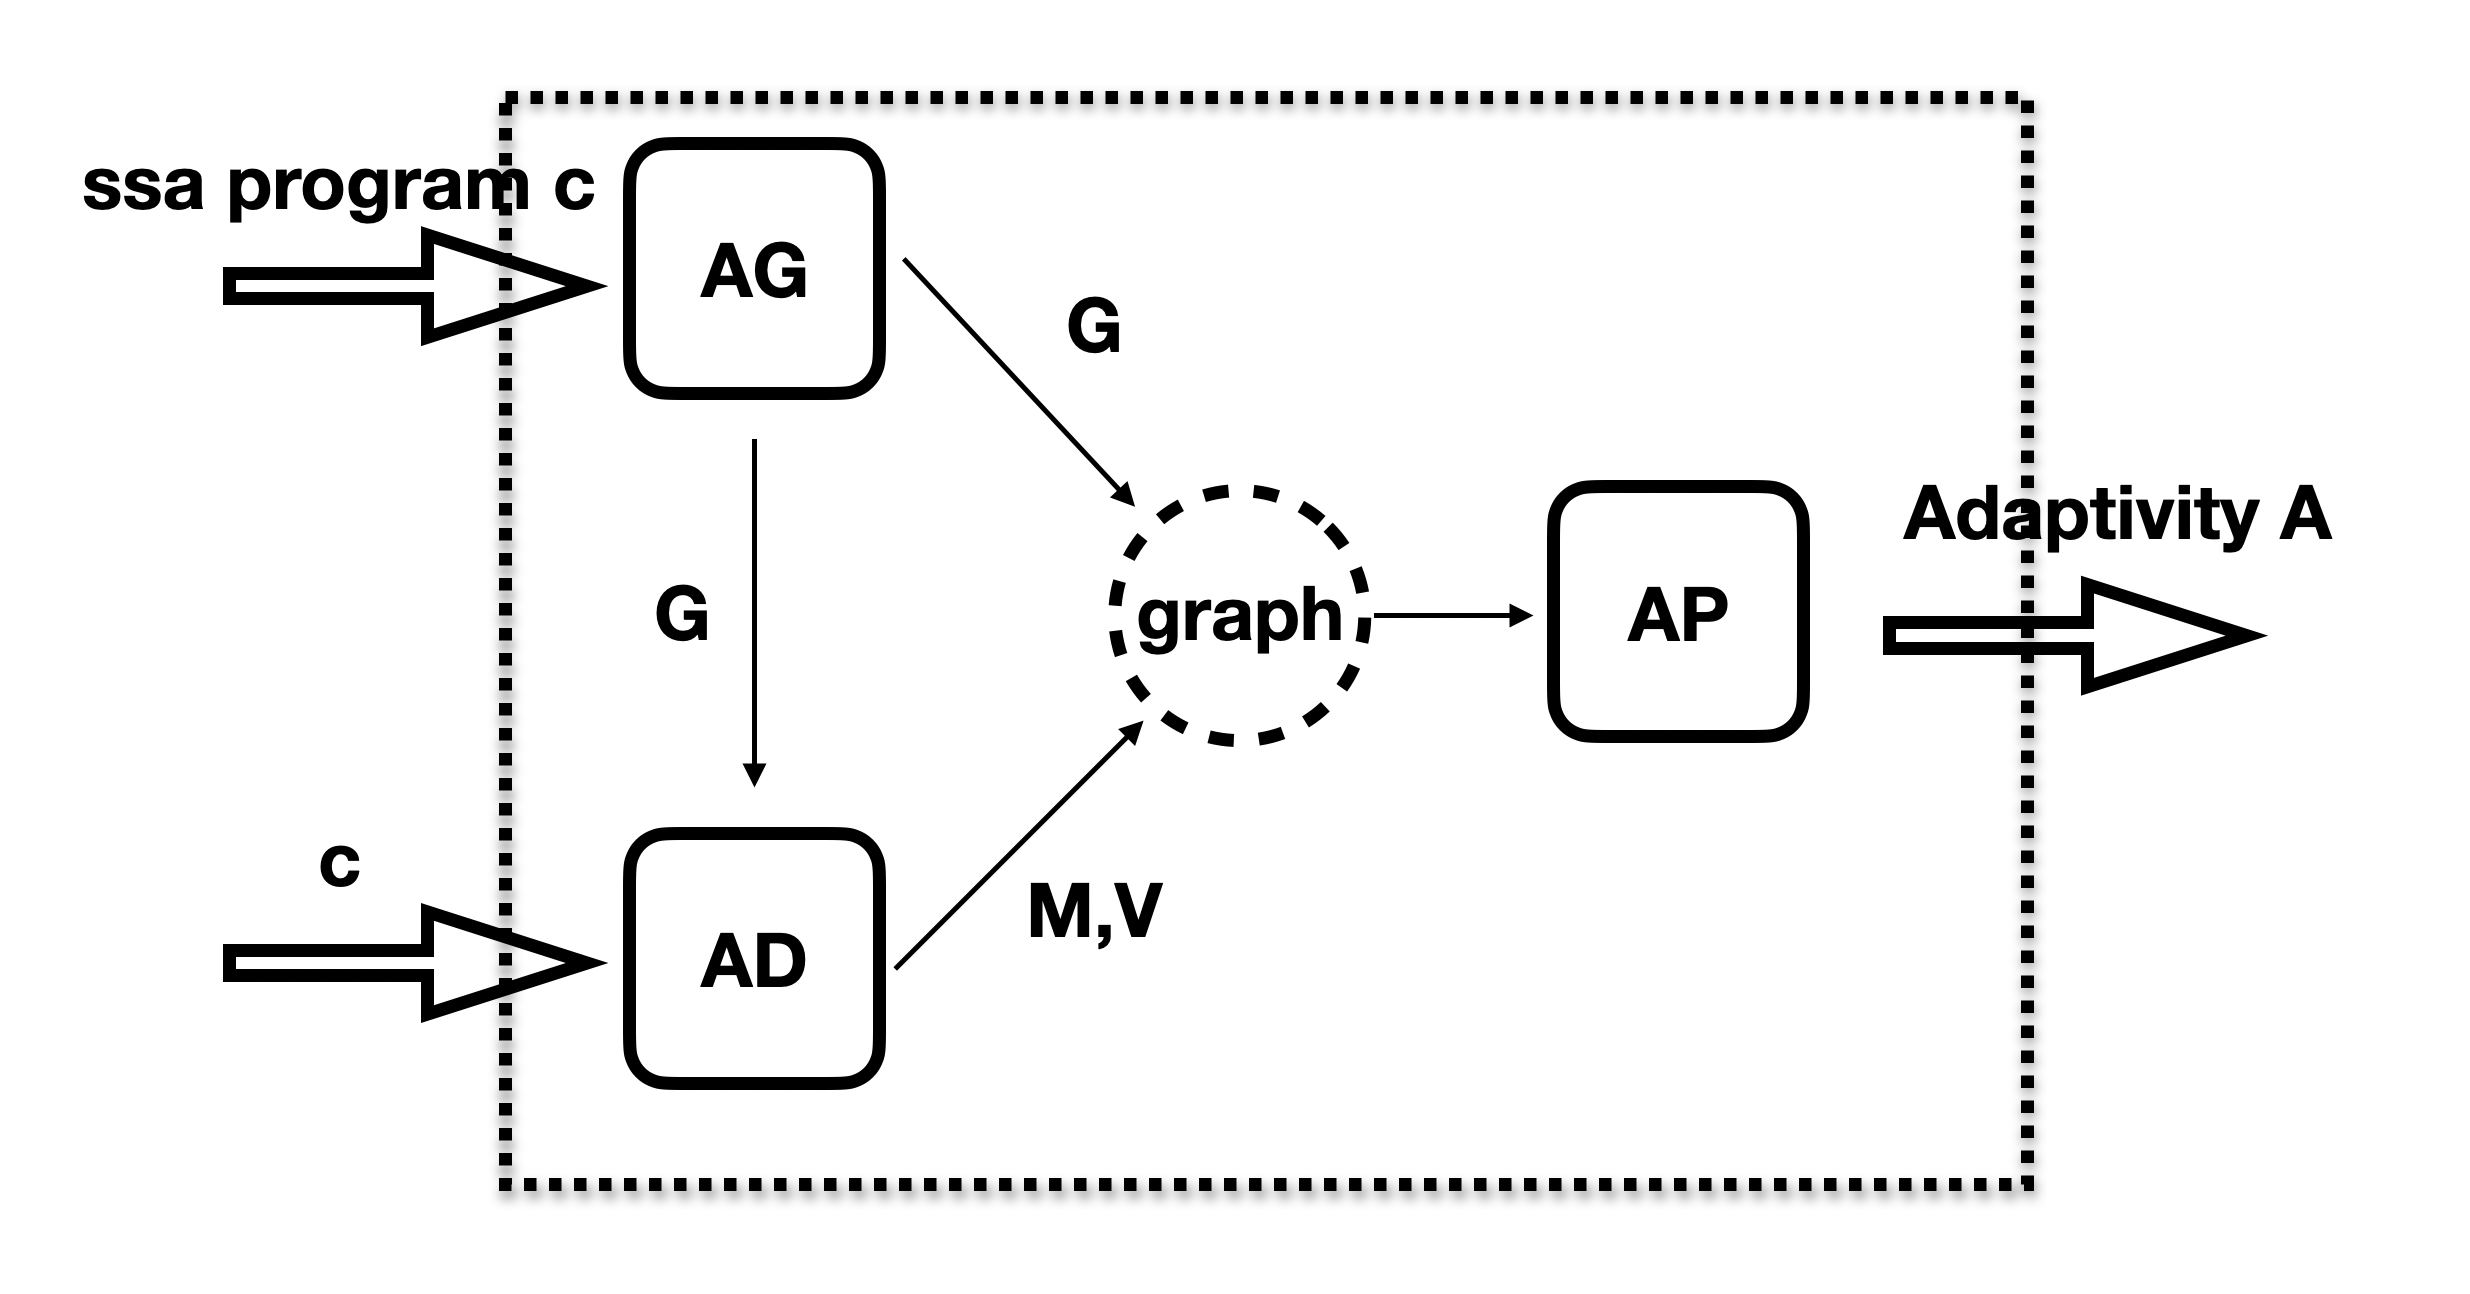
\includegraphics[width=0.7\columnwidth]{adapfun.png}
    \caption{The overview of {\THESYSTEM}}
    \label{fig:adaptfun}
\end{figure}


\subsection{Variable Estimation algorithm}
We first show how $G$ will be collected, through a variable estimating algorithm $\mathsf{AG}$ of the form $\ag{G; w; \ssa{c}}{ G'; w'} $ in Figure~\ref{fig:ag}. The input of $\mathsf{AG}$ is a list of estimated annotated variables $G$ collected before the program $\ssa{c}$, a while map $w$ consistent with previous estimation, a program $\ssa{c}$. The output of the algorithm is the updated global list $G'$, along with the updated while map $w$ for later estimation.   
\begin{figure}
 \begin{mathpar}
\inferrule
{
}
{ \ag{G ;w; \ssa{[\assign {x}{\expr}]^{l}}}{G ++ [\ssa{x}^{(l,w)}];w}
% G ;w; \ssa{[\assign {x}{\expr}]^{l}} \to G ++ [x^{(l,w)}];w 
}
~\textbf{ag-asgn}
\and
\inferrule
{
}
{ \ag{G ;w;  [ \assign{\ssa{x}}{q(\ssa{\expr})}]^{l}}{  G ++ [\ssa{x}^{(l,w)}] ; w} 
}~\textbf{ag-query}
%
\and 
%
\inferrule
{
\ag{G; w; \ssa{c_1}}{  G_1;w_1}
\and 
 \ag{G_1;w ; \ssa{c_2}}{  G_2; w_2}
 \\
 {G_3 = G_2 ++ \ssa{[\bar{x}^{(l,w)}]++ \ssa{[\bar{y}^{(l,w)}]}++ \ssa{[\bar{z}^{(l,w)}]} }}
}
{
\ag{G; w;
[\eif(\ssa{\bexpr},[ \bar{\ssa{x}}, \bar{\ssa{x_1}}, \bar{\ssa{x_2}}] ,[ \bar{\ssa{y}}, \bar{\ssa{y_1}}, \bar{\ssa{y_2}}],[ \bar{\ssa{z}}, \bar{\ssa{z_1}}, \bar{\ssa{z_2}}], \ssa{ c_1, c_2)}]^{l} }{ G_3 ;w}
}~\textbf{ag-if}
%
%
%
\and 
%
\inferrule
{
\ag{G; w; \ssa{c_1}}{ G_1; w_1}
\and 
\ag{G_1;w_1; \ssa{c_2}}{ G_2; w_2}
}
{
\ag{G; w;
\ssa{(c_1 ; c_2)}}{  G_2 ; w_2}
}
~\textbf{ag-seq}
\and 
\inferrule
{
{G_0 = G \quad w_0 =w }
\and
\forall 0 \leq z < N. 
{ \ag{ G_z ++ \ssa{[\bar{x}^{(l, {w_z}+l)}]} ; (w_z+l); \ssa{c}}{ G_{z+1} ; w_{z+1}}  }
\\
{G_f = G_N ++ \ssa{[\bar{x}^{(l, w_N \setminus l)}]} }
\and
{ \ssa{\aexpr} =  {N}  }
}
{\ag{G; w; [\eloop ~ \ssa{\aexpr}, n, [\bar{\ssa{x}}, \bar{\ssa{x_1}}, \bar{\ssa{x_2}}] ~ \edo ~ \ssa{c}]^{l} }{ G_f; w_N\setminus l }
}~\textbf{ag-loop}
% \and 
% \inferrule
% {
% \Gamma \vdash^{(i,i+a )}_{M, V} c 
% }
% {\Gamma \vdash^{(i, i+ N*a)}_{M_{i,a}^N(f), V_{i, a}^N} 
% \ewhile([\bexpr]^l,   c) : \phi \Rightarrow \psi
% }~\textbf{while}
% %
% \and
% %
% \inferrule
% {
% }
% { \ag{ G;w; [ \eswitch(\ssa{\expr}, \ssa{x},(\ssa{v_j} \rightarrow \ssa{q_j} ) )]^{l} } { G ++ [\ssa{x}^{(l, w)}] ; w} }
% ~\textbf{switch}
\end{mathpar}
 \caption{The algorithm $\mathsf{AG}$ }
    \label{fig:ag}
\end{figure}
The assignment is the source of variables $\mathsf{AG}$ estimates, in the case $\textbf{ag-asgn}$ and $\textbf{ag-query}$, the output global list is extended by $\ssa{x}^{(l,w)}$. When it comes to the if command in the rule $\textbf{ag-if}$, variables assigned in the then branch $\ssa{c_1}$, as well as the variables assigned in the else branch $\ssa{c_2}$, and the new generated variables $\bar{\ssa{x}},\bar{\ssa{y}},\bar{\ssa{z}}$ in $ [ \bar{\ssa{x}}, \bar{\ssa{x_1}}, \bar{\ssa{x_2}}] ,[ \bar{\ssa{y}}, \bar{\ssa{y_1}}, \bar{\ssa{y_2}}],[ \bar{\ssa{z}}, \bar{\ssa{z_1}}, \bar{\ssa{z_2}}]$. The sequence is standard by accumulating the predicted variables in the two commands $\ssa{c_1}$ and $\ssa{c_2}$ in a sequence $\ssa{c_1;c_2}$. The loop considers the loop iterations as well by assuming the loop counter $\ssa{\aexpr}$ to be certain natural number $N$ in the rule $\textbf{ag-loop}$. The algorithm counts the assigned variables in every iteration, including those new assigned variables in $\bar{\ssa{x}}$, those variables assigned in the body $\ssa{c}$, with the appropriate annotation showing the iteration number of the variables.      


\subsection{Matrix and Vector based algorithm}
We have a global list $G$ after the first scan of the ssa programs $\ssa{c}$. We develop a matrix and vector based approach based on the global list $G$ to get an estimated upper bound on the adaptivity of the program.  In this approach, a matrix is constructed according to those estimated annotated variables from the global list, in which every row and every column corresponds to the unique variable in $G$ by position. To be precise, in this matrix, $0$ means no dependency while non-zero value in the matrix shows may-dependency between corresponding variables. If the value of $M[i][j]$ in the matrix $M$ is greater than zero, we know annotated variable $G[i]$ may depend on $G[j]$. A vector $V$ has the same size as $G$ and it records whether the corresponding variable $G[i]$ is assigned with a query request. $V[i] =1$ means assigned with a query request and  otherwise $V[i]=0$. We call this algorithm which tracks may-dependency in the ssa programs and query information, $\mathsf{AD}$. The algorithm of the form $ \ad{\Gamma; \ssa{c} ;i }{ M; V;  i' } $, the input is a tuple consisting of three elements: (1) a one-row-N-column matrix $\Gamma$ storing the dependency from previous program, it is used when handling the if command. (2) the ssa program $\ssa{c}$ to be analyzed (3) an index $i$ specifying the location of the first assigned variable of the program $\ssa{c}$ in the global list $G$. The output of $\mathsf{AD}$ also consists of three elements ; (1) A matrix $M$ showing the may-dependency in $\ssa{c}$ (2) A vector $V$ records the query requests in $\ssa{c}$ (3) the index $i'$ that refers to the next position of the last assigned variable in $\ssa{c}$, if exists. The existence of the index $i'$ helps to locate the first assigned variable if we need to analyze programs after $\ssa{c}$.  

We first define some functions which use the indices in $G$. 
The function $\mathsf{L(i)}$ generates one-column-N-rows  matrix, where only the $i-th$ row is $1$ and all the other rows are $0$. This function is used to locate the right row when calculate the matrix when analyzing assignment and query. 

The function $\mathsf{R(e, i)}$ generates a one-row-N-column matrix. For every variable used in $e$, it finds the corresponding index $i$ in $G$ so that $G[i]$ maps to the variable and mark the $i$th column as $1$. If it is not found, we do not mark. When we say $G[i]$ maps to a target variable, we take off the annotation of $G[i]$ and check if the left variable is the same as the target variable. To handle loop, for instance, a variable $y$ appears many times in $G$, but with different annotations(iteration numbers), the argument $i$ helps to find most recent assignment variable $y$ before the index $i$ in $G$. It is still used when analyzing assignment and query. Thanks to our ssa language, our choice of the most recent assigned variable is reasonable because the variable used in the loop refers to the most recent assignment and every variable is uniquely assigned in its ssa form. 

We define $M_1;M_2$ to combine two matrix, where $M_1 + M_2$ is the standard sum of two matrix.
\[
M_1 ; M_2  :=  M_2 \cdot M_1 + M_1 + M_2 
\]
And define the operator $\uplus$ to combine two vectors.
\[
V_1 \uplus V_2  :=  \left\{
\begin{array}{ll}
1 & (V_1[i] = 1 \lor V_2[i] = 1) \land i = 1, \cdots, N \land |V_1| = |V_2|\\
0 & o.w.
\end{array}\right.
\]
For the sake of brevity, we also define some annotations as follows. We show how the algorithm $\mathsf{AD}$ handles the extra part $[ \bar{\ssa{x}}, \bar{\ssa{x_1}},\bar{\ssa{x_2}} ] $ in the if and loop commands. First, we give a unique name for variables in lists $\bar{\ssa{x}}, \bar{\ssa{x_1}}, \bar{\ssa{x_2}}$ respectively, as follows: {$ \forall 0 \leq z < |\bar{\ssa{x}}|. \bar{\ssa{x}}(z) = \ssa{x_z}, \bar{\ssa{x_1}}(z) = \ssa{x_{1z}}, \bar{\ssa{x_2}}(z) = \ssa{x_{2z}} $ }. And then we treat every tuple $(\ssa{x_z},\ssa{x_{1z}},\ssa{x_{2z}} )$ in $[\bar{\ssa{x}}, \bar{\ssa{x_1}}, \bar{\ssa{x_2}} ]$ as the simple may dependency case : $\ssa{x_z}$ may depend on both $ \ssa{x_{1z}}$ and $\ssa{x_{2z}}$, just like $ \assign{\ssa{x_z} }{\ssa{x_{1z}} + \ssa{x_{2z}} }$, defined as follows. 
$
 \ad{\Gamma; [\bar{\ssa{x}}, \bar{\ssa{x_1}}, \bar{\ssa{x_2}} ] ; i }{ M; V_{\emptyset}; i + |\bar{\ssa{x}}| } 
  \triangleq { \forall 0 \leq z < |\bar{\ssa{x}}|.
  \ad{\Gamma;\assign{\ssa{x_z} }{\ssa{x_{1z}} + \ssa{x_{2z}} }; i+z }{ M_{x_z};  V_{\emptyset}; i+z+1} }$
   where $M = \sum_{o \leq z < |\bar{\ssa{x}}| }M_{x_z} $.
% \framebox{$ \ad{\Gamma; \ssa{c} ; i_1){M;V;i_2} $}
%
\begin{figure}
\begin{mathpar}
\inferrule
{M = \mathsf{L}(i) * ( \mathsf{R}(\ssa{\expr},i) + \Gamma )
}
{
 \ad{\Gamma;[\assign {\ssa{x}}{\ssa{\expr}} ]^{l}; i }{M; V_{\emptyset}; i+1 }
% \Gamma \vdash_{M, V_{\emptyset}}^{(i, i+1)} [\assign {\ssa{x}}{\ssa{\expr}} ]^{l}
}
~\textbf{ad-asgn}
\and
\inferrule
{M = \mathsf{L}(i) * ( \mathsf{R}(\ssa{\expr},i) + \Gamma )
\\
V= \mathsf{L}(i)
}
{ 
\ad{\Gamma;[ \assign{\ssa{x}}{q(\ssa{\expr})} ]^{l} ; i }{M;V;i+1}
%  \vdash^{(i, i+1)}_{M, V} [ \assign{\ssa{x}}{q(\ssa{\expr})} ]^{l} 
}~\textbf{ad-query}
%
\and 
%
\inferrule
{
{\ad{\Gamma + \mathsf{R}(\ssa{\bexpr}, i_1); \ssa{c_1} ; i_1 }{ M_1;V_1;i_2 }}
% \Gamma + \mathsf{R}(\bexpr, i_1) \vdash^{(i_1, i_2)}_{M_1, V_1} \ssa{c_1} 
% : \Phi \land \bexpr \Rightarrow \Psi
\and 
{\ad{\Gamma + \mathsf{R}(\ssa{\bexpr}, i_1);\ssa{c_2} ; i_2 }{ M_2; V_2 ;i_3}}
% \Gamma + \mathsf{R}(\ssa{\bexpr}, i_1) \vdash^{(i_2, i_3)}_{M_2, V_2} \ssa{c_2} 
% : \Phi \land \neg \bexpr \Rightarrow \Psi
\\
% { \forall 0 \leq j < |\bar{x}|. \bar{x}(j) = x_j, \bar{x_1}(j) = x_{1j}, \bar{x_2}(j) = x_{2j}  }
{\ad{\Gamma; [ \bar{\ssa{x}}, \bar{\ssa{x_1}}, \bar{\ssa{x_2}}]; i_3 }{ M_x; V_{\emptyset}; i_3+|\bar{\ssa{x}}| }}
%
\and
%
{\ad{\Gamma; [ \bar{\ssa{y}}, \bar{\ssa{y_1}}, \bar{\ssa{y_2}}]; i_3+|\bar{\ssa{x}}| }{ M_y; V_{\emptyset}; i_3+|\bar{\ssa{x}}|+|\bar{\ssa{y}}| }}
%
\\
%
{\ad{\Gamma; [ \bar{\ssa{z}}, \bar{\ssa{z_1}}, \bar{\ssa{z_2}}]; i_3+|\bar{\ssa{x}}|+ |\bar{\ssa{y}}|}{ M_y; V_{\emptyset}; i_3+|\bar{\ssa{x}}|+|\bar{\ssa{y}}| + |\bar{\ssa{z}}| }}
% { \forall 0 \leq j < |\bar{x}|.  \Gamma \vdash_{M_{x_j}, V_{\emptyset}}^{i_3+j, i_3+j+1 } x_j \leftarrow x_{1j} + x_{2j} }
% \and
% { \forall 0 \leq j < |\bar{y}|.  \Gamma \vdash_{M_{y_j}, V_{\emptyset}}^{i_3+|\bar{x}|+j, i_3+|\bar{x}|+j+1 } y_j \leftarrow y_{1j} + y_{2j} }
% \\
% { \forall 0 \leq j < |\bar{z}|.  \Gamma \vdash_{M_{z_j}, V_{\emptyset}}^{i_3+|\bar{x}|+|\bar{y}|+j, i_3+|\bar{x}|+|\bar{y}|+j+1 } z_j \leftarrow z_{1j} + z_{2j} }
\\
{M = (M_1+M_2)+ M_x+M_y +M_z }
}
{
\Gamma \vdash^{(i_1, i_3+|\bar{x}|+|\bar{y}|+|\bar{z}|)}_{M, V_1 \uplus V_2 } 
[\eif(\ssa{\bexpr},[ \bar{\ssa{x}}, \bar{\ssa{x_1}}, \bar{\ssa{x_2}}] ,[ \bar{\ssa{y}}, \bar{\ssa{y_1}}, \bar{\ssa{y_2}}] , [ \bar{\ssa{z}}, \bar{\ssa{z_1}}, \bar{\ssa{z_2}}] , \ssa{ c_1, c_2)}]^{l}
}~\textbf{ad-if}
%
%
%
\and 
%
\inferrule
{
{\ad{\Gamma; \ssa{c_1} ; i_1 }{ M_1 ; V_1; i_2 }  }
% \Gamma \vdash^{(i_1, i_2)}_{M_1, V_1} \ssa{c_1} 
% : \Phi \Rightarrow \Phi_1
\and 
{\ad{\Gamma;\ssa{c_2}; i_2}{M_2; V_2 ;i_3 }}
% \Gamma \vdash^{(i_2, i_3)}_{M_2, V_2} \ssa{c_2} 
% : \Phi_1 \Rightarrow \Psi 
}
{
\ad{\Gamma ; (\ssa{c_1 ; c_2} ) ; i_1}{(M_1 {;} M_2) ; V_1 \uplus V_2 ; i_3  }
% \Gamma \vdash^{(i_1, i_3)}_{M_1 {;} M_2, V_1 \uplus V_2}
% \ssa{c_1 ; c_2} 
% : \Phi \Rightarrow \Psi
}
~\textbf{ad-seq}
\and 
\inferrule
{
B= |\ssa{\bar{x}}| \and {A = |\ssa{c}|}
% \and
% {\Gamma \vdash^{(i, i+B)}_{M_{10}, V_{10}} [\bar{\ssa{x}}, \bar{\ssa{x_1}}, \bar{\ssa{x_2}}] }
% \and
% {\Gamma \vdash^{(i+B,i+B+A )}_{M_{20}, V_{20}} \ssa{c} 
% }
\\
\forall 0 \leq j < N. 
{\ad{\Gamma;[\bar{\ssa{x}}, \bar{\ssa{x_1}}, \bar{\ssa{x_2}}]; i+ j*(B+A) }{M_{1j};V_{1j}; i+B+j*(B+A) }}
% {\Gamma \vdash^{(i+j*(B+A), i+B+j*(B+A))}_{M_{1j}, V_{1j}}  } [\bar{\ssa{x}}, \bar{\ssa{x_1}}, \bar{\ssa{x_2}}]
\\
{
\ad{\Gamma;\ssa{c} ; i+B+j*(B+A)  }{M_{2j}; V_{2j}; i+B+A+j*(B+A) }
% \Gamma \vdash^{(i+B+j*(B+A),i+B+A+j*(B+A) )}_{M_{2j}, V_{2j}} \ssa{c} 
% : \Phi \land e_n = \lceil{z+1}\rceil \Rightarrow \Psi 
}
\\
{
\ad{\Gamma ; [\bar{\ssa{x}}, \bar{\ssa{x_1}}, \bar{\ssa{x_2}}] ; i+N*(B+A) }{M; V ;i+N*(B+A)+B}
% \Gamma \vdash^{(i+N*(B+A) ,i+N*(B+A)+B )}_{M, V} [\bar{\ssa{x}}, \bar{\ssa{x_1}}, \bar{\ssa{x_2}}]
% : \Psi \Rightarrow \Phi \land e_N = \lceil{z}\rceil 
}
\\
{ \ssa{\aexpr} =  {N}  }
\and
{M' = M+ \sum_{0 \leq j <N}( M_{1j}+M_{2j})  }
\and
{V' = V \uplus \sum_{0 \leq j <N}( V_{1j} \uplus V_{2j})  }
}
{\Gamma \vdash^{(i, i+N*(B+A)+B   )}_{M', V'} 
[\eloop ~ \ssa{\aexpr}, 0, [\bar{\ssa{x}}, \bar{\ssa{x_1}}, \bar{\ssa{x_2}}] ~ \edo ~ \ssa{c}]^{l}
% : \Phi \land \expr_N = \lceil { N} \rceil \Rightarrow \Phi \land \expr_N = \lceil{0}\rceil
}~\textbf{ad-loop}
% \and 
% \inferrule
% {
% \Gamma \vdash^{(i,i+a )}_{M, V} c 
% }
% {\Gamma \vdash^{(i, i+ N*a)}_{M_{i,a}^N(f), V_{i, a}^N} 
% \ewhile([\bexpr]^l,   c) : \phi \Rightarrow \psi
% }~\textbf{while}
% %
% \and
% %
% \inferrule
% { \Gamma + \mathsf{R}(\expr,i) \vdash^{(i, i+1)}_{M, V} \assign{ x}{q_j} 
% % : \Phi \Rightarrow \Psi
% \\
% j \in \{1, \dots, N\}     }
% {\Gamma \vdash^{(i, i+1)}_{ M,V } 
% [\eswitch(\ssa{\expr}, \ssa{x},(v_j \rightarrow q_j ) ]^{l}
% % : \Phi \Rightarrow \Psi 
% }
% ~\textbf{switch}
% %
% \and
% %
% \inferrule
% { 
% \vDash 
% \Phi \Rightarrow \Phi'  
% \and
% \Gamma \vdash^{(i_1, i_2)}_{(M',V')} c : \Phi' \Rightarrow \Psi'
% \and
% \vDash \Psi' \Rightarrow \Psi
% \and 
% \Phi \vDash M' \leq M
% \and 
% \Phi \vDash V' \leq V
% }
% {\Gamma \vdash^{(i_1, i_2)}_{(M,V)} c 
% : \Phi \Rightarrow \Psi
% }
% ~\textbf{conseq}
\end{mathpar}
    \caption{The algorithm AD}
    \label{fig:algo_ad}
\end{figure}
One of the key idea under algorithm $\mathsf{AD}$ is to track the indices $i$,$i'$ both in the input and output to synchronize with its previous algorithm $\mathsf{AG}$. The index in $\mathsf{AD}$ increases as the same way as the global list expands after the analysis of a program $\ssa{c}$, which helps $\mathsf{AD}$ record the dependency relation from the program $\ssa{c}$ in the right place of the matrix. For example, in the case $\textbf{ad-asgn}$ and $\textbf{ad-query}$, the index increases by 1, which corresponds to their counterparts of algorithm $\textbf{AG}$. The if and loop commands have the extra part $ [\bar{\ssa{x}}, \bar{\ssa{x_1}}, \bar{\ssa{x_2}}] $ and we find that the output index increases by also considering this part as we do in collecting the global list.  

Another interesting point is the construction of the matrix. The fundamental case is the assignment and query cases. We use a function $L(i)$ to generate a N-row-one-column matrix $L$ to guarantee the resulting matrix only has non-zeros at row $i$. The intuition behind is that one single assignment or query request can only reveal the dependency of its assigned variable (corresponding to one row of the matrix) to the variables used on the right hand sides. Thanks to the index $i$, we know which row this assignment should be in the matrix. The function $\mathsf{R}(\ssa{\expr},i)$ gets a one-row-N-column matrix marking the variables used in the right hand side. The $\Gamma$ is designed for the if command and we will discuss it later. We can see one simple example $sa$ to get a taste.     
\[
sa \triangleq
\begin{array}{l}
    \left[x_1 \leftarrow 2 \right]^1; \\
    \left[x_2 \leftarrow x_1 + 2 \right]^2 ; \\
    \left[x_3 \leftarrow x_1 + x_2 \right]^3
\end{array}
\]
In the program $sa$, only simple assignment is involved. When we assume $\Gamma$ is empty, for the assignment at line $3$, the matrix is built as follows.
\[
\textbf{line3:} ~~
 \left[x_3 \leftarrow x_1 + x_2 \right]^3 :
 ~~~
\begin{blockarray}{cc}
\begin{block}{c[c]}
 x_1 & 0   \\
 x_2 & 0 \\
 x_3 & 1 \\
\end{block}
\end{blockarray}
*
\begin{blockarray}{ccc}
x_1 & x_2 & x_3 \\
\begin{block}{[ccc]}
1 & 1 & 0 \\
\end{block}
\end{blockarray}
= 
\begin{blockarray}{cccc}
& x_1 & x_2 & x_3\\
\begin{block}{c[ccc]}
x_1 & 0 & 0 & 0 \\
x_2 & 1 & 0 & 0 \\
x_3 & 1 & 1 & 0 \\
\end{block}
\end{blockarray}
\]
% a simple example of assignment
% \begin{example}[Simple Assignment]
% \[
% SA \triangleq
% \begin{array}{l}
%     \left[x_1 \leftarrow 2 \right]^1; \\
%     \left[x_2 \leftarrow x_1 + 2 \right]^2 ; \\
%     \left[x_3 \leftarrow x_1 + x_2 \right]^3
% \end{array}
% \]
% %
% %
% \[
%  \textbf{line2:} ~~
%  \left[x_2 \leftarrow x_1 + 2 \right]^2 :
%  ~~~
% \begin{blockarray}{cc}
% \begin{block}{c[c]}
%  x_1 & 0   \\
%  x_2 & 1 \\
%  x_3 & 0 \\
% \end{block}
% \end{blockarray}
% *
% \begin{blockarray}{ccc}
% x_1 & x_2 & x_3 \\
% \begin{block}{[ccc]}
% 1 & 0 & 0 \\
% \end{block}
% \end{blockarray}
% = 
% \begin{blockarray}{cccc}
% & x_1 & x_2 & x_3\\
% \begin{block}{c[ccc]}
% x_1 & 0 & 0 & 0 \\
% x_2 & 1 & 0 & 0 \\
% x_3 & 0 & 0 & 0 \\
% \end{block}
% \end{blockarray}
% \]
% %
% %
% %
% \[
% \textbf{line3:} ~~
%  \left[x_3 \leftarrow x_1 + x_2 \right]^3 :
%  ~~~
% \begin{blockarray}{cc}
% \begin{block}{c[c]}
%  x_1 & 0   \\
%  x_2 & 0 \\
%  x_3 & 1 \\
% \end{block}
% \end{blockarray}
% *
% \begin{blockarray}{ccc}
% x_1 & x_2 & x_3 \\
% \begin{block}{[ccc]}
% 1 & 1 & 0 \\
% \end{block}
% \end{blockarray}
% = 
% \begin{blockarray}{cccc}
% & x_1 & x_2 & x_3\\
% \begin{block}{c[ccc]}
% x_1 & 0 & 0 & 0 \\
% x_2 & 1 & 0 & 0 \\
% x_3 & 1 & 1 & 0 \\
% \end{block}
% \end{blockarray}
% \]
% %
% \end{example}
 We use a one-row-N-column matrix $\Gamma$ as one of the input of $\mathsf{AD}$, to handle the cases when the control flow diverges in the labelled if command $[\eif(\ssa{\bexpr},[ \bar{\ssa{x}}, \bar{\ssa{x_1}}, \bar{\ssa{x_2}}] ,[ \bar{\ssa{y}}, \bar{\ssa{y_1}}, \bar{\ssa{y_2}}] , [ \bar{\ssa{z}}, \bar{\ssa{z_1}}, \bar{\ssa{z_2}}] , \ssa{ c_1, c_2)}]^{l} $, where the execution of either branch may depend on the conditional guard $\ssa{\bexpr}$. Follow this intuition, the analysis of either branch is supposed to consider the variables used in the conditional $\ssa{\bexpr}$, tracked in $\Gamma$. In the case $\textbf{ad-if}$, we can see the analysis of the two branches $\ssa{c_1}$ and $\ssa{c_2}$ share the same input $\Gamma + \mathsf{R}(\ssa{\bexpr}, i)$ and $\mathsf{R}(\ssa{\bexpr}, i) $ tells the variables assigned before the if command and used in the conditional $\ssa{\bexpr}$.   

We compose the matrix and vectors in the case of sequence in $\textbf{ad-seq}$. The non-zeros or we call it effect range of the matrix and vector is decided by its input and output indices. From the case $\textbf{ad-seq}$, two programs $\ssa{c_1}$ and $\ssa{c_2}$ have disjoint effect ranges $[i_1, i_2)$ and $[i_1,i_3)$, it is safe to combine them without lose information. 

The loop case is handled in a well organized way. We use $B= |\bar{\ssa{x}}|$ and $A= |{\ssa{c}}|$ to estimate the size of variables assigned in $\bar{\ssa{x}}$ and $\ssa{c}$. And  $|\ssa{c}|$ is defined by the help of the algorithm $\mathsf{AG}$, defined as $|\ssa{c}|= |G|$ when $\ag{[];\ssa{c};\emptyset }{ G; \emptyset }$. The algorithm then gets how many iterations $N$ the loop may executes from the loop counter $\ssa{\aexpr}$. For every iteration, it first records the dependency relations between variables in $ [\bar{\ssa{x}}, \bar{\ssa{x_1}}, \bar{\ssa{x_2}}]$ by constructing a corresponding matrix $M_{1j}$ ($j$ is the iteration number) and an empty vector $V_{1j}$, and analyze the loop body $\ssa{c}$ with a resulting matrix $M_{2j}$ and vector $V_{2j}$. We give an extra analysis of those new assigned variables as what $\mathsf{AG}$ does, it works well when the loop is executed ($N = 0$) or not. We know that for all the possible iteration number $j$, $M_{1j}$ and $M_{2j}$ have disjoint effect ranges so we combine them, similar as the vectors $V_{1j}$ and $V_{2j}$.   

Finally, we are able to construct a variable-based weighted dependency graph based on $G$,$M$ and $V$ generated by the framework. The definition of the estimated adaptivity is the weight of the most weighted path in the graph defined as follows. 

\begin{defn}
[Estimated Adaptivity]
Given a program $\ssa{c}$, the global list $G$, and $\ad{\Gamma; \ssa{c}; i_1}{M, V, i_2}$, the weighted dependency graph $G_{ssa}(M, V,G,i_1,i_2) = (Nodes, Edges, Weights)$ is defined as:
\\
Nodes $Vt = \{ G(j) \in \mathcal{LV} \mid i_1 \leq j < i_2 \}$
\\
Edges $E = \{ (G(j_1), G(j_2)) \in \mathcal{LV} \times \mathcal{LV} \mid M[j_1][j_2] \geq 1 \land  i_1 \leq j_1,j_2 < i_2   \}$
\\
 Weights $Wt = \{ (  G(j), 1 ) \in \mathcal{LV} \times \mathcal{N} | i_1 \leq j < i_2 \land V[j] = 1\}
        \cup \{ (  G(j), 0 ) \in \mathcal{LV} \times \mathcal{N} | i_1 \leq j < i_2 \land V[j] = 0 \} $.
        
Adaptivity of the program defined according to the graph is as:
\[
Adapt(M, V,i_1,i_2) := \max_{vt_1, vt_2 \in Vt}\{ \mathsf{Weight}( p(vt_1, vt_2), Wt) \},
\]
where $p(k, l)$ is the path in graph $G_{ssa}(M, V, i_1,i_2)$ starting from $k$ to $l$, $\mathsf{Weight}(p(vt_1,vt_2), Wt)$ get the total sum of weights along the path $p(vt_1,vt_2)$.
\end{defn}        

\subsection{Analysis on two round algorithm}
We show how {\THESYSTEM} analyze the two round algorithm. For the sake of brevity, we conduct the analysis on the simplified two round algorithm $TR^{ssa}$.

% \[
% TR^{ssa}(k) \triangleq
% {
% \begin{array}{l}
%     % \left[j \leftarrow 0 \right]^1 ; \\
%     \clabel{a_1 \leftarrow []}^{1} ; \\
%     \clabel{\assign{j_1}{0} }^{2} ; \\
%     \eloop ~ \clabel{k}^{3} ~ \edo [(j_3, j_1,j_2),(a_3, a_1,a_2)]~ \\
%     \Big(
%     \clabel{ x_1 \leftarrow q(\chi(j_3)\cdot \chi(k))}^{4}  ; \\
%     \clabel{ \assign{j_2}{j_3+1} }^{5} ;\\
%     \clabel{a_2 \leftarrow x_1 :: a_3}^{6}       \Big);\\
%     \clabel{l_1 \leftarrow q(\mathrm{sign}\big (\sum_{i\in [k]} \chi(i)\times\ln\frac{1+a_3[i]}{1-a_3[i]} \big ))}^{7}\\
% \end{array}
% }
% \]
{\THESYSTEM} first runs the algorithm $\mathsf{AG}$ to generate the global list $G$. We assume the input $k=2$ and have the following.

\[G_{k=2} = \left[
  {a_1}^{(1,\emptyset)} , {a_3}^{(2,[2:1])} , {x_1}^{(3,[2:1])} , {a_2}^{(4,[2:1])} ,  {a_3}^{(2,[2:2])} , {x_1}^{(3,[2:2])} , {a_2}^{(4,[2:2])} , {a_3}^{(2,\emptyset)} , {l_1}^{(5,\emptyset)}   \right] \]
% \[G_{k=2} = \left[ \begin{array}{l}
%      {a_1}^{(1,\emptyset)} , {j_1}^{(2,\emptyset)}, {j_3}^{(3,[2:1])} , {a_3}^{(3,[2:1])} , {x_1}^{(4,[2:1])} ,{j_2}^{(5,[2:1])} ,
%   {a_2}^{(6,[2:1])},  \\
%     {j_3}^{(3,[2:2])} , {a_3}^{(3,[2:2])} , {x_1}^{(4,[2:2])} ,{j_2}^{(5,[2:2])} ,
%   {a_2}^{(6,[2:2])},
%   {j_3}^{(3,\emptyset)} , {a_3}^{(3,\emptyset)} ,
%   {l_1}^{(7,\emptyset)} \\  
% \end{array}
%      \right] \]
 We denote $a_1^{1}$ short for ${a_1}^{(1,\emptyset)}$ and ${a_3}^{(2,1)}$ short for ${a_3}^{(2,[2:1])}$. Then the resulting matrix $M_{tr}$ and $V_{tr}$ of the algorithm $\mathsf{AD}$ as follows.
 
{ \tiny
 \[
M_{tr} =  \left[ \begin{matrix}
 & a_1^{1} & a_3^{(2,1)} & x_1^{(3,1)} & a_2^{(4,1)}  & a_3^{(2,2)} & x_1^{(3,2)} & a_2^{(4,2)} & a_3^{2} & l_1^{5}\\
 a_1^{1} & 0 & 0 & 0 & 0 & 0 & 0 & 0 &0 &0 \\
a_3^{(2,1)} & 1 & 0 & 0 & 0 & 0 & 0 & 0&0&0\\
x_1^{(3,1)} & 0 & 0 & 0 & 0 & 0 & 0& 0& 0 &0\\
a_2^{(4,1)} & 0 & 1 & 1 & 0 & 0 & 0 & 0& 0&0\\
a_3^{(2,2)} & 1 & 0 & 0 & 1 & 0 & 0 & 0 & 0&0 \\
x_1^{(3,2)} & 0 & 0 & 0 & 0 & 0 & 0 & 0& 0&0\\
a_2^{(4,2)} & 0 & 0 & 0 & 0 & 1 & 1 & 0& 0&0\\
a_3^{2} & 1 & 0 & 0 & 0 & 0 & 0 & 1& 0&0\\
l_1^{5} & 0 & 0 & 0 & 0 & 0 & 0 & 0 & 1 &0 \\
 \end{matrix} \right] 
~ , V_{tr} = \left [ \begin{matrix}
a_1^{1} &  0 \\
a_3^{(2,1)} & 0 \\
x_1^{(3,1)} & 1 \\
a_2^{(4,1)} &  0 \\
a_3^{(2,2)} & 0 \\
x_1^{(3,2)} & 1 \\
a_2^{(4,2)} &  0 \\
a_3^{2} &  0 \\
l_1^{5} &  1 \\
\end{matrix} \right ]
\]
}
%% a graph is better here

\subsection{ Soundness of {\THESYSTEM}}
We would like to show that the query-based dependency graph generated from the trace of the execution of the target ssa program is a subgraph of the variable-based dependency graph predicted from our algorithm ${\THESYSTEM}$, and the query requested during the execution is also bounded by an estimation from our algorithm.

We first give a definition of subgraph of a query-based dependency graph with respect to a variable-based dependency graph.
\begin{defn}
[Subgraph]
Given a query-based dependency graph $G_{s} = (V_1, E_1)$, a variable-based dependency graph $G_{ssa} = (V_2, E_2)$, $G_{s} \subseteq G_{ssa}$ iff:\\
$\exists f$ so that \\
1. for every $v \in V_1$, $f(v) \in V_2$. 
\\
2. $\forall e=(v_i, v_j) \in E_1$, there exists a path 
% $g(e)$ 
from $f(v_i)$ to $f(v_2)$ in $G_{ssa}$.
\end{defn}

Then we show the soundness of {\THESYSTEM}. In the theorem, we use some definition. $G \vDash M, V$ says that $G$ and $M$, $V$ have the corresponding size. $G; w \vDash (\ssa{c}, i_1,i_2)$ checks if the variables assigned in $\ssa{c}$ calculated by $\mathsf{AG}$ matches the variables in $G$ from index $i_1$ to $i_2$.

\begin{thm}
[Soundness of {\THESYSTEM}]
Given $ \ad{\Gamma; \ssa{c}; i_1 }{M; V;i_2}$,  for any global list $G$,  loop maps $w$ such that $G ;w \vDash (\ssa{c}, i_1, i_2) \land G \vDash (M,V)$. $K$ is the number of queries inquired during the execution of the piece of program $\ssa{c}$ and |V| gives the number of non-zeros in $V$. 
% $|.|_{low} $ is the annotation erasure, which turns a ssa form program $\ssa{c}$ to its low-level version.
Then,
\[
K \leq |V| \land \forall D, \ssa{m}. G_{s}(\ssa{c},D,\ssa{m},w) \subseteq G_{ssa}(M, V,G,i_1, i_2)
\]      
\end{thm}


\section{More examples}
The two round strategy works well in our framework, we explore further to look at an advanced adaptive data analysis algorithm - multiple round algorithm.
\begin{example}[Two Round Algorithm]
    \[
    %
        \bf{TRC}(k) \triangleq
    \begin{array}{l}
           \clabel{ a \leftarrow []}^{1} ; \\
            \clabel{\assign{j}{k} }^{2} ; \\
            \ewhile ~ \clabel{j > 0}^{3} ~ \edo ~ \\
            \Big(
             \clabel{x \leftarrow (\chi(k - j)\cdot \chi(k)) }^{4}  ; \\
             \clabel{\assign{j}{j-1}}^{5} ;\\
            \clabel{a \leftarrow x :: a}^{6}       \Big);\\
            \clabel{l \leftarrow (\mathrm{sign}\big (\sum_{i\in [k]} \chi(i)\times\ln\frac{1+a[i]}{1-a[i]} \big ))}^{7}\\
        \end{array}
    \]
    %
    \begin{algorithm}
    \footnotesize
    \caption{A two-round analyst strategy for random data (The example in  \cite{dwork2015preserving})}
    \label{alg:twoRound}
    \begin{algorithmic}
    \REQUIRE Mechanism $\mathcal{M}$ with a hidden state $X\in [N]^{n}$ sampled u.a.r., control set size $c$
    % \STATE Define control dataset $C = \{0,1, \cdots, c - 1\}$
    % \STATE Initialize $Nscore(i) = 0$ for $i \in [N]$, $I = \emptyset$ and $Cscore(C(i)) = 0$ for $i \in [c]$
    % \STATE  {\bf for}\ $j\in [k]$\ {\bf do} 
    % \STATE \qquad {\bf let} $p=\uniform(0,1)$ 
    % \STATE \qquad {\bf define} $q (x) = \bernoulli ( p )$ .
    % \STATE \qquad {\bf define} $qc (x) = \bernoulli ( p )$ .
    % \STATE \qquad {\bf let} $a = \mathcal{M}(q)$ 
    % \STATE \qquad {\bf for}\ $i \in [N]$\ {\bf do}
    % \STATE \qquad \qquad $Nscore(i) = Nscore(i) + (a - p)*(q (i) - p)$ if $i \notin I$
    % \STATE \qquad {\bf for}\ $i \in [c]$\ {\bf do}
    % \STATE \qquad \qquad $Cscore(C(i)) = Cscore(C(i)) + (a - p)*(qc (i) - p)$
    % \STATE \qquad {\bf let} $I = \{i | i\in [N] \land Nscore(i) > \max(Cscore)\}$
    % \STATE \qquad {\bf let} $X = X \setminus I$ 
    \RETURN $X$.
    % \ENSURE 
    \end{algorithmic}
    \end{algorithm}
    %
%
    \end{example}

\begin{example}[Multiple Round Algorithm]
%
\[
%
MR(k) \triangleq
\begin{array}{l}
     \left[j \leftarrow k \right]^1 ; \\
    \left[I_1 \leftarrow [] \right]^2; \\
    \ewhile ~ \clabel{j > 0}^{3} ~ \edo ~ \\
    \Big(
    \clabel{\assign{j}{j-1}}^{4} ;\\
    \left[p_1 \leftarrow c \right]^5; \\
    \left[ a_1 \leftarrow q (p, I_3) \right]^6;\\
    \left[I_2 \leftarrow \mathrel{\mathsf{update}} ( {I_3}, (a_1, p_1))  \right]^7
    \Big) 
\end{array}
\]
%
\begin{algorithm}
\footnotesize
\caption{A multi-round analyst strategy for random data base \cite{dwork2015preserving}}
\label{alg:multiRound}
\begin{algorithmic}
\REQUIRE Mechanism $\mathcal{M}$ with a hidden state $X\in [N]^{n}$ sampled u.a.r., control set size $c$
\STATE Define control dataset $C = \{0,1, \cdots, c - 1\}$
\STATE Initialize $Nscore(i) = 0$ for $i \in [N]$, $I = \emptyset$ and $Cscore(C(i)) = 0$ for $i \in [c]$
\STATE  {\bf for}\ $j\in [k]$\ {\bf do} 
\STATE \qquad {\bf let} $p=\uniform(0,1)$ 
\STATE \qquad {\bf define} $q (x) = \bernoulli ( p )$ .
\STATE \qquad {\bf define} $qc (x) = \bernoulli ( p )$ .
\STATE \qquad {\bf let} $a = \mathcal{M}(q)$ 
\STATE \qquad {\bf for}\ $i \in [N]$\ {\bf do}
\STATE \qquad \qquad $Nscore(i) = Nscore(i) + (a - p)*(q (i) - p)$ if $i \notin I$
\STATE \qquad {\bf for}\ $i \in [c]$\ {\bf do}
\STATE \qquad \qquad $Cscore(C(i)) = Cscore(C(i)) + (a - p)*(qc (i) - p)$
\STATE \qquad {\bf let} $I = \{i | i\in [N] \land Nscore(i) > \max(Cscore)\}$
\STATE \qquad {\bf let} $X = X \setminus I$ 
\RETURN $X$.
\end{algorithmic}
\end{algorithm}
%
%
\end{example}
%   We have seen the two round algorithm in Section~\ref{subsec:loop-syntax}. We show the multiple-round algorithm, which is an advanced algorithm.
%  \\
\textbf{Description:}
The multiple round algorithm starts from an initialized empty tracking list $I$, a score called Nscore $ns=0$ , another score Cscore $cs=0$. There is a hidden database $X$ as well.
It goes $k$ rounds and every round, the two scores $ns$ and $cs$ are updated by a query result. Then the list $I$ is updated by the two scores for every round. After the $r$ rounds, the algorithm returns the columns of the hidden database $X$ not specified in the tracking list $I$, which is $X\setminus I$. 

The algorithm is written in the loop language as $MR$. 
It uses a loop for the $k$ rounds computation and. We use functions $update\_nscore(p,a)$,$update\_cscore(p,a)$,$update(I,ns,cs)$ to simplify the complex update computation of Nscore, Cscore and the tracking list $I$. It will not change our analysis because these functions provides enough information through their arguments.
% As described in the two round algorithm, the multi-round algorithm has a loop as well.
% compare to two round algorithm
In comparison with the two round algorithm, the query asked in each iteration is not independent  in the multiple round one any more. 
The query in one iteration $j$ now depends on the tracking list $I$ from its previous iteration $j-1$, which is updated by the query result at the same iteration $j-1$. We can easily see the connection between queries from different iterations.
% the result of the query from previous iteration,
% so that the query ask at the $j^{th}$ iteration is
% $q(p, I)$.
%
%
%
%
\begin{figure}
\begin{center}
%
\begin{tikzpicture}[scale=\textwidth/17cm,samples=200]
%%% The nodes represents the k query in the first round
\filldraw[red] (0, 3) circle (2pt) node [anchor=south]{$a_1^{(4,1)}$};
\filldraw[black] (3, 4) circle (2pt) node [anchor=south]{$p_1^{(3,1)}$};
% \filldraw[black] (6, 2) circle (2pt) node [anchor=south]{$q^4_3$};
\filldraw[black] (6, 4) circle (2pt) node [anchor=south]{$p_1^{(3,2)}$};
\filldraw[black] (8, 3) circle (2pt) node [anchor=south]{$I_3^{(2,1)}$};
%%%%%% The nodes represents the n^k queries in the second round
\filldraw[red] (0, 2) circle (2pt) node [anchor=north]{$a_1^{(4,2)}$};
\filldraw[black] (3, 0) circle (2pt) node [anchor=north]{$I_2^{(5,1)}$};
% \filldraw[black] (6, 0) circle (2pt) node [anchor=north]{$q^{3, 7}_{k+1}$};
\filldraw[black] (6, 0) circle (2pt) node [anchor=north]{$I_2^{(5,2)}$};
\filldraw[black] (8, 1) circle (2pt) node [anchor=north]{$I_3^{(2,3)}$};
\filldraw[black] (8, 2) circle (2pt) node [anchor=south]{$I_3^{(2,2)}$};
\filldraw[black] (12, 2) circle (2pt) node [anchor=south]{$I_1^{1}$};
%%%%%The edges between a and I
%%%%% (a1(4,1), I3(2,1))
\draw[very thick, ->] (0, 3)  -- (7.9, 3) ;
%%%%% (a1(4,2), I3(2,2))
\draw[very thick, ->] (0, 2)  -- (7.9, 2) ;
%%%%%% The edges represents their dependency relations GROUP between I3 and I1
\draw[very thick,<-] (12, 2)  -- (8, 2) ;
\draw[very thick,->] (8, 2) -- (3.1, 0) ;
%
\draw[very thick,<-] (12, 2)  -- (8, 1) ;
\draw[very thick,->] (8, 1) -- (6.1, 0) ;
%
\draw[very thick,<-] (12, 2)  -- (8, 3) ;
%
%%%%%% The edges represents their dependency relations GROUP between I2 and others
%%%%%% The edges represents their dependency relations GROUP between I2(5,1) and others
\draw[very thick, ->] (3, 0)  -- (0, 2.9) ;
\draw[very thick, ->] (3, 0)  -- (3, 3.9) ;
\draw[very thick, ->] (3, 0)  -- (7.9, 2.9) ;
%%%%%% The edges represents their dependency relations GROUP between I2(5,2) and others
\draw[very thick, ->] (6, 0)  -- (0, 1.9) ;
\draw[very thick, ->] (6, 0)  -- (6, 3.9) ;
\draw[very thick, ->] (6, 0)  -- (7.9, 1.9) ;
%%%% The longest path representing the adaptivity
\draw[ultra thick, red, ->, dashed] (0, 2) -- (7.9, 2);
\draw[ultra thick, red, ->, dashed] (8, 2) -- (3.1, 0);
\draw[ultra thick, red, ->, dashed] (3, 0)  -- (0, 2.9);
\end{tikzpicture}
\end{center}
    \caption{the variable dependency graph for multi round algorithm}
    \label{fig:multi-round-graph-ssa}
\end{figure}
%
The adaptivity is 1 computed from the graph.
The query-based dependency graph is a subgraph of the variable dependency graph for multi round algorithm.



\begin{example}[Simple Seq]
    %
    %
    \[
    %
        \kw{seq} \triangleq 
    \begin{array}{l} 
           \clabel{ \assign{x}{\chi[0]}}^{1} ; \\
            \clabel{\assign{y}{\chi[x + 1]} }^{2} ; \\
            \clabel{\assign{z}{\chi[y + 1]}}^{3}; \\
             \clabel{\assign{w}{\chi[z + 1] \cdot \chi[x]} }^{4}  ; \\
        \end{array}
    \]
    \end{example}

    \begin{example}[If with Data-Value Dependency Separated]
        %
        %
        \[
        %
        \begin{array}{l}
        \kw{if-value-dependency} \triangleq \\
           \quad \clabel{ \assign{x}{\chi[0]}}^{1} ; \\
           \quad \clabel{\assign{z}{\chi[1]} }^{2} ; \\
           \quad \eif(\clabel{x < 0}, \\
           \quad \clabel{\assign{y}{\chi[z]}}^{3}, 
           \quad \clabel{\assign{y}{\chi[0]}}^{4})
            \end{array}
        \]
        \end{example}

        \begin{example}[If with Data-Control Dependency Overlapped]
            %
            %
            \[
            %
            \begin{array}{l}
            \kw{if-control-dependency} \triangleq \\
                \clabel{ \assign{x}{\chi[0]}}^{1} ; \\
                \clabel{\assign{z}{\chi[1]} }^{2} ; \\
                \eif(\clabel{x < 0}^{3}, 
                \clabel{\assign{y}{\chi[0] + \chi[1]}}^{4}, 
                \clabel{\assign{y}{\chi[0]}}^{4})
            \end{array}
            \]
            \end{example}


            \begin{example}[Simple While with Recursive Data-Value Dependency]
                %
                %
                \[
                %
                \kw{while}() \triangleq
                \begin{array}{l}
                    \clabel{ \assign{a}{\chi[0]}}^{1} ; \\
                    \clabel{\assign{j}{10000} }^{2} ; \\
                        \ewhile ~ \clabel{j > 0}^{3} ~ \edo ~ \\
                        \Big(
                         \clabel{\assign{x}{\query(\chi[a]) }}^{4}  ; \\
                         \clabel{\assign{j}{j-1}}^{5} ;\\
                        \clabel{a \leftarrow x + a}^{6}       \Big);
                    \end{array}
                \]
                \end{example}
%
        \begin{example}[Simple While with Multi-Path Data-Value Dependency]
        %
        %
        \[
        %
        \begin{array}{l}
        \kw{while-multiple-path}(k) \triangleq \\
            \clabel{ \assign{x}{\query(\chi[0])}}^{1} ; \\
            \clabel{\assign{j}{k} }^{2} ; \\
                \ewhile ~ \clabel{j > 0}^{3} ~ \edo ~ \\
                \Big(
                 \clabel{\assign{j}{j-1}}^{4} ;\\
                 \eif(\clabel{j \% 2 == 0}^{5}, 
                 \clabel{\assign{y}{\chi[x]}}^{6}, 
                 \clabel{\assign{w}{\chi[x]}}^{7})                             
                 \clabel{\assign{x}{\query(\chi(\ln(y)))} }^{7} \Big);
            \end{array}
        \]
        \end{example}
%
        \begin{example}[Simple While with Recursive Multiple-Variable Data-Value Dependency]
            \[
            %
            \begin{array}{l}
            \kw{while-multiple-var}(k) \triangleq \\
                \clabel{ \assign{x}{\query(\chi[0])}}^{1} ; \\
                \clabel{ \assign{y}{\query(\chi[1])}}^{2} ; \\
                \clabel{\assign{j}{k} }^{3} ; \\
                    \ewhile ~ \clabel{j > 0}^{4} ~ \edo ~ \\
                    \Big(
                     \clabel{\assign{j}{j-1}}^{5} ;\\
                     \clabel{\assign{z}{\query(\chi(x + \ln(y)))} }^{6}  ; \\
                     \clabel{ \assign{x}{\query(\chi[z])}}^{7} ; \\
                     \clabel{ \assign{y}{\query(\chi[z])}}^{8} ; \\
                    \Big);
                \end{array}
            \]
            \end{example}
            %
            %
            \begin{example}[Simple While with Data-Value and Data-Control Dependency]
                %
                \[
                \begin{array}{l}
                \kw{while-value-control-dependency}() \triangleq \\
                    \clabel{ \assign{x}{\query(\chi[0])} }^{1} ; \\
                    \clabel{ \assign{z}{\query(\chi[0])} }^{2} ; \\
                        \ewhile ~ \clabel{x > 0}^{3} ~ \edo ~ \\
                        \Big(
                        \clabel{\assign{x}{\query(\chi(z))} }^{4}  ; \\
                        \clabel{\assign{z}{\query(\chi(x))}}^{5} ;
                      \Big);
                    \end{array}
                \]
                \end{example}
%
            \begin{example}[Simple While with MultiplePath Data-Value and Data-Control Dependency]
                %
                \[
                    %
                    \begin{array}{l}
                    \kw{while-multiple-path-value-control-dependency}(k) \triangleq\\
                        \clabel{ \assign{x}{\query(\chi[0])}}^{1} ; \\
                        \clabel{\assign{y}{0} }^{2} ; \\
                            \ewhile ~ \clabel{x > 0}^{3} ~ \edo ~ \\
                            \Big(
                             \clabel{\assign{x}{x-1}}^{4} ;\\
                             \eif(\clabel{y > 0}^{5}, 
                             \clabel{\assign{y}{\query(\chi[12])}}^{6}, 
                             \clabel{\assign{w}{\query(\chi[9])}}^{7})                             
                             \Big);\\
                             \clabel{\assign{y}{\query(\chi(\ln(y)))} }^{8} 
                        \end{array}
                    \]
                \end{example}
                                %
                \begin{example}[Nested While with Recursive Data-Value Dependency]
                    %
                    %
                    \[
                    %
                    \begin{array}{l}
                    \kw{nest-while-value-dependency}(k) \triangleq \\
                        \clabel{ \assign{x}{\query(\chi[0])}}^{1} ; \\
                        \clabel{\assign{j}{k} }^{2} ; \\
                            \ewhile ~ \clabel{j > 0}^{3} ~ \edo ~ \\
                            \Big(
                             \clabel{\assign{y}{\query(\chi(\ln(x)))} }^{4}  ; \\
                             \clabel{\assign{j}{j-1}}^{5} ;\\
                             \clabel{\assign{i}{k}}^{6} ;\\
                             \ewhile ~ \clabel{i > 0}^{7} ~ \edo ~ \\
                             \Big(
                              \clabel{\assign{x}{\query(\chi(\ln(x)))} }^{8}  ; \\
                              \clabel{\assign{i}{i-1}}^{9}
                              \Big) \Big);
                        \end{array}
                    \]
                    \end{example}

                    \begin{example}[Nested While with Nested Recursive Data-Value Dependency Across Outer and Inner Loop]
                        %
                        %
                        \[
                        %
                        \begin{array}{l}
                            \kw{nestedWhileRecAcross}(k) \triangleq \\
                            \clabel{ \assign{x}{\query(\chi[0])}}^{1} ; \\
                            \clabel{\assign{j}{k} }^{2} ; \\
                                \ewhile ~ \clabel{j > 0}^{3} ~ \edo ~ \\
                                \Big(
                                 \clabel{\assign{y}{\query(\chi(\ln(x)))} }^{4}  ; \\
                                 \clabel{\assign{j}{j-1}}^{5} ;\\
                                 \clabel{\assign{i}{k}}^{6} ;\\
                                 \ewhile ~ \clabel{i > 0}^{7} ~ \edo ~ \\
                                 \Big(
                                  \clabel{\assign{x}{\query(\chi(\ln(y)))} }^{8}  ; \\
                                  \clabel{\assign{i}{i-1}}^{9}
                                  \Big) \Big);
                            \end{array}
                        \]
                        \end{example}
                %
            
                        \begin{example}[Nested While with Nested Recursive Multiple Variable 
                            Data-Value Dependency Across Outer and Inner Loop]
                            %
                            \[
                            %
                            \begin{array}{l}
                            \kw{nestedWhileMultiVarRecAcross}(k) \triangleq \\
                                \clabel{ \assign{x}{\query(\chi[0])}}^{1} ; \\
                                \clabel{ \assign{y}{\query(\chi[1])}}^{2} ; \\
                                \clabel{\assign{j}{k} }^{3} ; \\
                                    \ewhile ~ \clabel{j > 0}^{3} ~ \edo ~ \\
                                    \Big(
                                     \clabel{\assign{y}{\query(\chi(\ln(x) + y))} }^{4}  ; \\
                                     \clabel{\assign{j}{j-1}}^{5} ;\\
                                     \clabel{\assign{i}{k}}^{6} ;\\
                                     \ewhile ~ \clabel{i > 0}^{7} ~ \edo ~ \\
                                     \Big(
                                      \clabel{\assign{x}{\query(\chi(\ln(y))+\chi[x])} }^{8}  ; \\
                                      \clabel{\assign{i}{i-1}}^{9}
                                      \Big) \Big);
                                \end{array}
                            \]
                            \end{example}
                    
                            

\section{Related Works}

%% Acknowledgments
\begin{acks}                            %% acks environment is optional
                                        %% contents suppressed with 'anonymous'
  %% Commands \grantsponsor{<sponsorID>}{<name>}{<url>} and
  %% \grantnum[<url>]{<sponsorID>}{<number>} should be used to
  %% acknowledge financial support and will be used by metadata
  %% extraction tools.
  This material is based upon work supported by the
  \grantsponsor{GS100000001}{National Science
    Foundation}{http://dx.doi.org/10.13039/100000001} under Grant
  No.~\grantnum{GS100000001}{nnnnnnn} and Grant
  No.~\grantnum{GS100000001}{mmmmmmm}.  Any opinions, findings, and
  conclusions or recommendations expressed in this material are those
  of the author and do not necessarily reflect the views of the
  National Science Foundation.
\end{acks}


% Bibliography
\bibliography{main}


%% Appendix
\appendix
\section{Appendix}

Text of appendix \ldots

\end{document}
